\documentclass[a4paper,10pt]{article}
\usepackage[utf8]{inputenc}
\usepackage{hyperref}
\usepackage{array}
\usepackage{lastpage}
\usepackage{lipsum}
\usepackage{multirow}  
\usepackage{fancyhdr}
\usepackage[hmargin=2cm,top=4cm,headheight=65pt,footskip=65pt]{geometry}
\usepackage{xcolor, colortbl}
\usepackage{geometry}
\usepackage{graphicx} 
\usepackage{lastpage}
\usepackage{fontspec}
\setmainfont{Arial}
\usepackage{caption}
\usepackage{float}
\usepackage{parskip}
\usepackage{amsmath}
% Set up margins

\renewcommand{\headrulewidth}{0pt}
\definecolor{JBOGrey}{HTML}{8e8778}  
\definecolor{JBOGreen}{HTML}{008f85}  

\fancyhead[CE,CO,LE,LO,RE,RO]{} 

\fancyhead[C]{ % Centered header
    \arrayrulecolor{JBOGrey} 
    \begin{tabular}{|m{3cm}|m{6cm}|m{4cm}|m{1cm}|m{1cm}|}
        \hline
        % Row 1
        \multirow{3}{*}{
            \makebox[2.7cm][c]{ % Ensures horizontal centering with specified width
                \raisebox{0pt}[1.5cm][0pt]{ % Adjust height for vertical centering
                    
\includegraphics[width=3.3cm]{JBO_logo.jpg}
                }
            }
        }  
        & \multirow{3}{*}{
            \makebox[167pt][c]{ % Ensures horizontal centering within the multirow
                \raisebox{0pt}[1cm][0pt]{ % Adjust height for vertical centering
                    \shortstack{
                        {\fontsize{11}{16.5}\selectfont Technical Note } \\
                        {\textcolor{JBOGreen}{\fontsize{10}{15}\selectfont \textit{ Hindcast Evaluation for Monopile \newline Design }}}
                    }
                }
            }
        }
        % col 2
        & \centering 
            \raisebox{0pt}[0.5cm][0pt]{ % Adjust the vertical space here
                \shortstack{
                    {\fontsize{6}{9}\selectfont Employer Number} \\ 
                    {\fontsize{7}{10.5}\selectfont \textbf{ 01 }}} 
            }
        % col 3
        & \multicolumn{2}{c|}{\centering 
            \raisebox{0pt}[0.6cm][0pt]{ % Adjust this to match column 2
                \shortstack{
                    {\fontsize{6}{9}\selectfont Issued on} \\
                    {\fontsize{7}{10.5}\selectfont \textbf{ 14.09.2023 }}}}} 
        \\ 
        
        % Row 2
        \cline{3-5} 
        % col 1
        & % skipped because multirow    
        % col 2
        & \centering 
            \raisebox{0pt}[0.6cm][0pt]{ % Adjust this to maintain vertical centering
                \shortstack{
                    {\fontsize{6}{9}\selectfont Reference Number} \\
                    {\fontsize{7}{10.5}\selectfont \textbf{ 99Z999-JBO-TNHDCD-EN-3001 }}}        
            }
        % col 3
        & \multicolumn{2}{c|}{
            \centering \fontsize{9}{13.5}\selectfont \textbf{Revision}}  \\
         
        % Row 3
        \cline{3-3} 
        % col 1
        &  % skipped because multirow    
        % col 2
        & \centering 
            \raisebox{0pt}[0.6cm][0pt]{ % Adjust this to maintain vertical centering
                \shortstack{
                    {\fontsize{6}{9}\selectfont Status}  \\
                    {\fontsize{7}{10.5}\selectfont \textbf{ DRA }}}    
            }
        % col 3
        & \centering  
            \raisebox{0pt}[0.6cm][0pt]{ % Keep this consistent with other columns
                \shortstack{
                    {\fontsize{6}{9}\selectfont JBO} \\
                    {\fontsize{7}{10.5}\selectfont \textbf{ 01 }}}    
            }
        & \centering  
            \raisebox{0pt}[0.6cm][0pt]{ % Keep this consistent with other columns
                \shortstack{
                    {\fontsize{6}{9}\selectfont Employer} \\
                    {\fontsize{7}{10.5}\selectfont \textbf{ 01 }}}   
            } &
        
        \arrayrulecolor{JBOGreen} 
        \cline{1-5}
        \arrayrulecolor{JBOGrey} 
    \end{tabular}


}       

\fancyfoot[CE,CO,LE,LO,RE,RO]{}

\fancyfoot[C]{ % Centered footer
    \begin{tabular}{|m{1.4cm}|m{12cm}|m{2cm}|}
        \arrayrulecolor{JBOGreen} 
        \hline
        \arrayrulecolor{JBOGrey} 
        \makebox[1.4cm][c]{ % Ensure horizontal centering for "Chapter:"
            \raisebox{0pt}[0.4cm][0pt]{ % Adjust height for vertical centering
                {\fontsize{10}{13.8}\selectfont Chapter:}
            }
        }
        & \makebox[12cm][c]{ % Ensure horizontal centering for chapter title
            \raisebox{0pt}[0.4cm][0pt]{ % Adjust height for vertical centering
                {\fontsize{10}{13.8}\selectfont \leftmark}
            }
        }
        & \makebox[2cm][c]{ % Ensure horizontal centering for "Page:"
            \raisebox{0pt}[0.4cm][0pt]{ % Adjust height for vertical centering
                {\fontsize{10}{13.8}\selectfont Page: (\thepage/\pageref{LastPage})}
            }
        } \\
        \hline              
    \end{tabular}
}

\thispagestyle{fancy}

\fancypagestyle{titlepage}{
    \fancyhf{} 
    \fancyfoot[C]{
        \begin{tabular}{m{5cm} m{6cm} m{1.5cm} m{1.5cm} m{0.8cm} }
        \textcolor{JBOGreen}{\fontsize{10}{15}\selectfont \textbf{JBO Rev.}} &
        \textcolor{JBOGreen}{\fontsize{10}{15}\selectfont \textbf{Date}} &
        \textcolor{JBOGreen}{\fontsize{10}{15}\selectfont \textbf{Author}} &
        \textcolor{JBOGreen}{\fontsize{10}{15}\selectfont \textbf{QC}} &
        \textcolor{JBOGreen}{\fontsize{10}{15}\selectfont \textbf{App.}} 
        \\        
        \arrayrulecolor{JBOGreen} 
        \hline
        \fontsize{10}{15}\selectfont 01 &
        \fontsize{10}{15}\selectfont 14.09.2023 &
        \fontsize{10}{15}\selectfont ALa &
        \fontsize{10}{15}\selectfont FOs &
        \fontsize{10}{15}\selectfont FOs &

        \end{tabular}
    }
}

\begin{document}

\thispagestyle{titlepage} % Use custom footer for the title page

\begin{table}[]
    \begin{tabular}{|m{3.5cm}|m{6cm}|m{4cm}|m{1cm}|m{1cm}|m{1cm}|}
        \hline
        
        % Row 1
        \multicolumn{2}{|l|}{
            \makebox[9cm][l]{ % Ensures horizontal centering with specified width
                \raisebox{0pt}[2.5cm][0pt]{ % Adjust height for vertical centering
                    
\includegraphics[width=7.5cm]{JBO_logo.jpg}
                }
            }
        }
        & \multicolumn{4}{c|}{
            \makebox[6cm][c]{ % Ensures horizontal centering with specified width
                \centering
                \raisebox{30pt}[2.5cm][0pt]{ % Adjust height for vertical centering
                    \centering
                    {\textcolor{JBOGreen}{\fontsize{12}{14.4}\selectfont \textbf{Jörss - Blunck - Ordemann GmbH}}}
                    }
                }
            }
        
        \\
        \hline
        
        % Row 2
        \makebox[3cm][l]{ % 	Ensures horizontal centering with specified width
            \raisebox{2pt}[0.6cm][0pt]{ % Adjust height for vertical centering
                {\fontsize{10}{12}\selectfont Reference Number}
            }
        }
        & \multicolumn{2}{l|}{
            \makebox[9cm][l]{ % Ensures horizontal centering with specified width
                \raisebox{-1pt}[0cm][0pt]{ % Adjust height for vertical centering
                    {\fontsize{10}{12}\selectfont \textbf{ 99Z999-JBO-TNHDCD-EN-3001 }}
                }
            }
        } 
        & \multicolumn{2}{c|}{
            \makebox[1.8cm][l]{ % Ensures horizontal centering with specified width
                \raisebox{0pt}[0cm][0pt]{ % Adjust height for vertical centering
                    {\fontsize{10}{12}\selectfont \textbf{Revision}}
                }
            }
        }
        & \raisebox{-3pt}[0cm][0pt]{ % Keep this consistent with other columns
            \shortstack{
                {\fontsize{7}{8.4}\selectfont Status} \\
                {\fontsize{9}{10.8}\selectfont \textbf{ DRA }}
            }    
        }
        \\
        \hline
        
        % Row 3
        \makebox[3cm][l]{ % Ensures horizontal centering with specified width
            \raisebox{2pt}[0.6cm][0pt]{ % Adjust height for vertical centering
                {\fontsize{10}{5}\selectfont Employer Number }
            }
        }
        & \multicolumn{2}{l|}{
            \makebox[9cm][l]{ % Ensures horizontal centering with specified width
                \raisebox{0pt}[0cm][0pt]{ % Adjust height for vertical centering
                    {\fontsize{10}{5}\selectfont \textbf{ 01 }}
                }
            }
        } 
        & 
        \makebox[0.9cm][l]{ 
            \raisebox{-4pt}[0cm][0pt]{ % Keep this consistent with other columns
                \shortstack{
                    {\fontsize{7}{5}\selectfont JBO} \\
                    {\fontsize{9}{5}\selectfont \textbf{ 01 }}
                }
            }
        } 
        
        &
        \makebox[1cm][c]{ 
            \raisebox{-4pt}[0cm][0pt]{ % Keep this consistent with other columns
                \shortstack{
                    {\fontsize{7}{5}\selectfont Employer} \\
                    {\fontsize{9}{5}\selectfont \textbf{ 01 }}
                }
            }
        } 
        
        & 
        \makebox[1cm][c]{ 
            \raisebox{-4pt}[0cm][0pt]{ % Keep this consistent with other columns
                \shortstack{
                    {\fontsize{7}{5}\selectfont Page} \\
                    {\fontsize{9}{5}\selectfont \textbf{\thepage/\pageref{LastPage}}}
                }    
            }
        }
        \\
        \hline
        
        % Row 4
        \makebox[3cm][l]{ % Ensures horizontal centering with specified width
            \raisebox{3pt}[0.6cm][0pt]{ % Adjust height for vertical centering
                {\fontsize{10}{12}\selectfont Date of Issue}
            }
        }
        & \multicolumn{2}{l|}{
            \makebox[9cm][l]{ % Ensures horizontal centering with specified width
                \raisebox{-1pt}[0.0cm][0pt]{ % Adjust height for vertical centering
                    {\fontsize{10}{12}\selectfont \textbf{ 14.09.2023 }}
                }
            }
        } 
        & \multicolumn{3}{c|}{
            \makebox[1.5cm][c]{ % Ensures horizontal centering with specified width
                \raisebox{-1pt}[0.0cm][0pt]{ % Adjust height for vertical centering
                    {\textcolor{JBOGreen}{\fontsize{10}{12}\selectfont \textbf{ Technical Note }}}
                }
            }
        }
        \\
        \hline
        
    \end{tabular}
\end{table}

\vspace*{1cm}

\begin{centering}
\includegraphics[width=0.4\textwidth]{__REPLACEMENT_PLACEHOLDER_12__} \\% Replace with actual image path \\
\end{centering}

\hspace{3.6cm}
\begin{minipage}{\textwidth}
\vspace{2cm}

\fontsize{14}{20}\selectfont \textbf{RWE} \\
\fontsize{20}{25}\selectfont \textbf{Offshore Wind Farm} \\
\\
\fontsize{18}{25}\selectfont \textbf{Technical Note} \\
\textcolor{JBOGreen}{\fontsize{16}{14.4}\selectfont \textit{\textbf{Hindcast Evaluation for Monopile \newline Design}}}
\end{minipage}




\pagestyle{fancy}

\section{Introduction}
\subsection{General}
For the support structure design of an offshore wind farm, the interpretation of the metocean data is required.
Hydrodynamic load analysis will be conducted on this basis, which basically follow the recommendations in ???  .
\\
\\
The here investigated project site is a generic site in the German North Sea. Monopile substructures are assumed to be derived as substructure type.

\subsection{Document purpose}
This document describes the marine assessment of metocean hindcast data to determine the hydrodynamic load impact in an
offshore wind project. The evaluated design parameter shall fulfil the requirements for a preliminary design phase of
substructure and foundation.
\section{Data Basis}
Here the underlying databasis is analysed. General information is shown in table REF:

\begin{figure}[H] 
 \centering 
 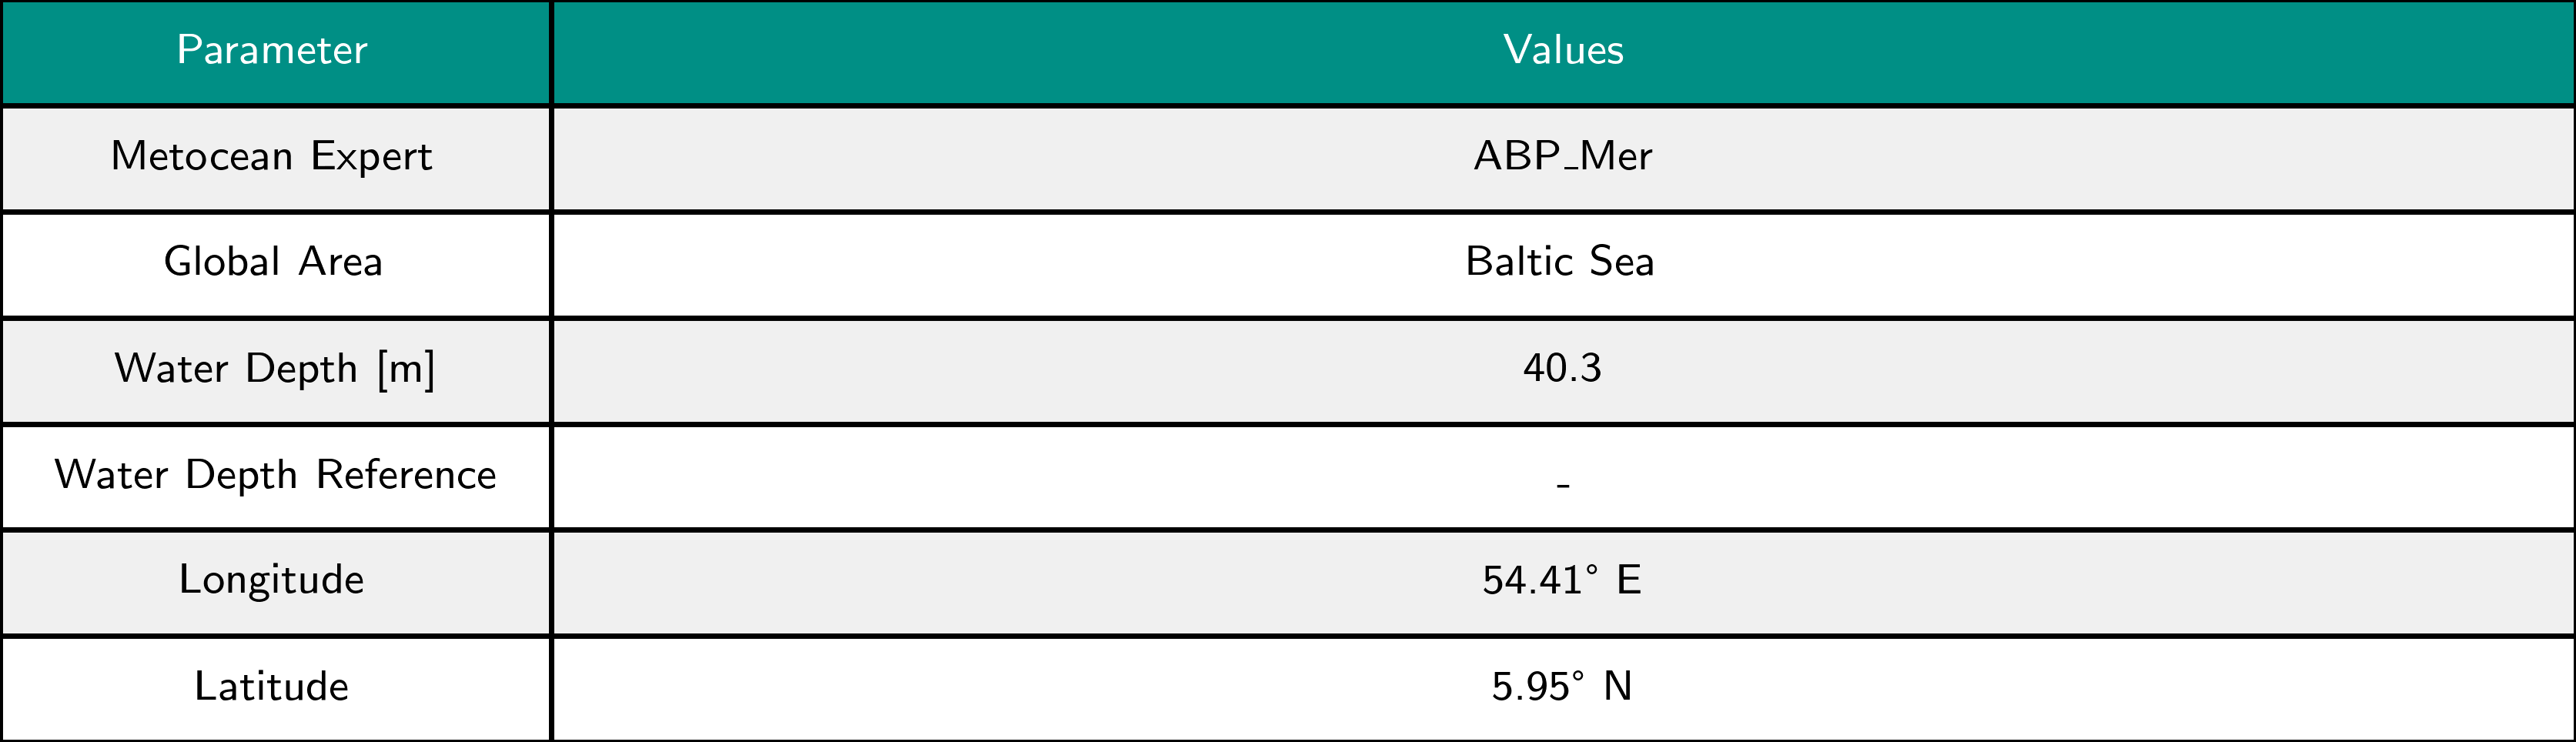
\includegraphics[width=1.0\textwidth ]{C:/Users/aaron.lange/Desktop/Projekte/Hindcast_Tool/HindTool/example_output/DataSorce_global_page_1.png} 
 \captionsetup{type=table} 
\caption{ DataSorce-global-page-1 } 
 \label{tab: DataSorce_global_page_1 } 
\end{figure}

\subsection{Data set overview}

Meta information of the time series data sets considered in this document are specified below in detail. A quality assurance including potential resampling or correction has been conducted. Analysed sensors in the data sets are tabulated in REFERENZ.

\begin{figure}[H] 
 \centering 
 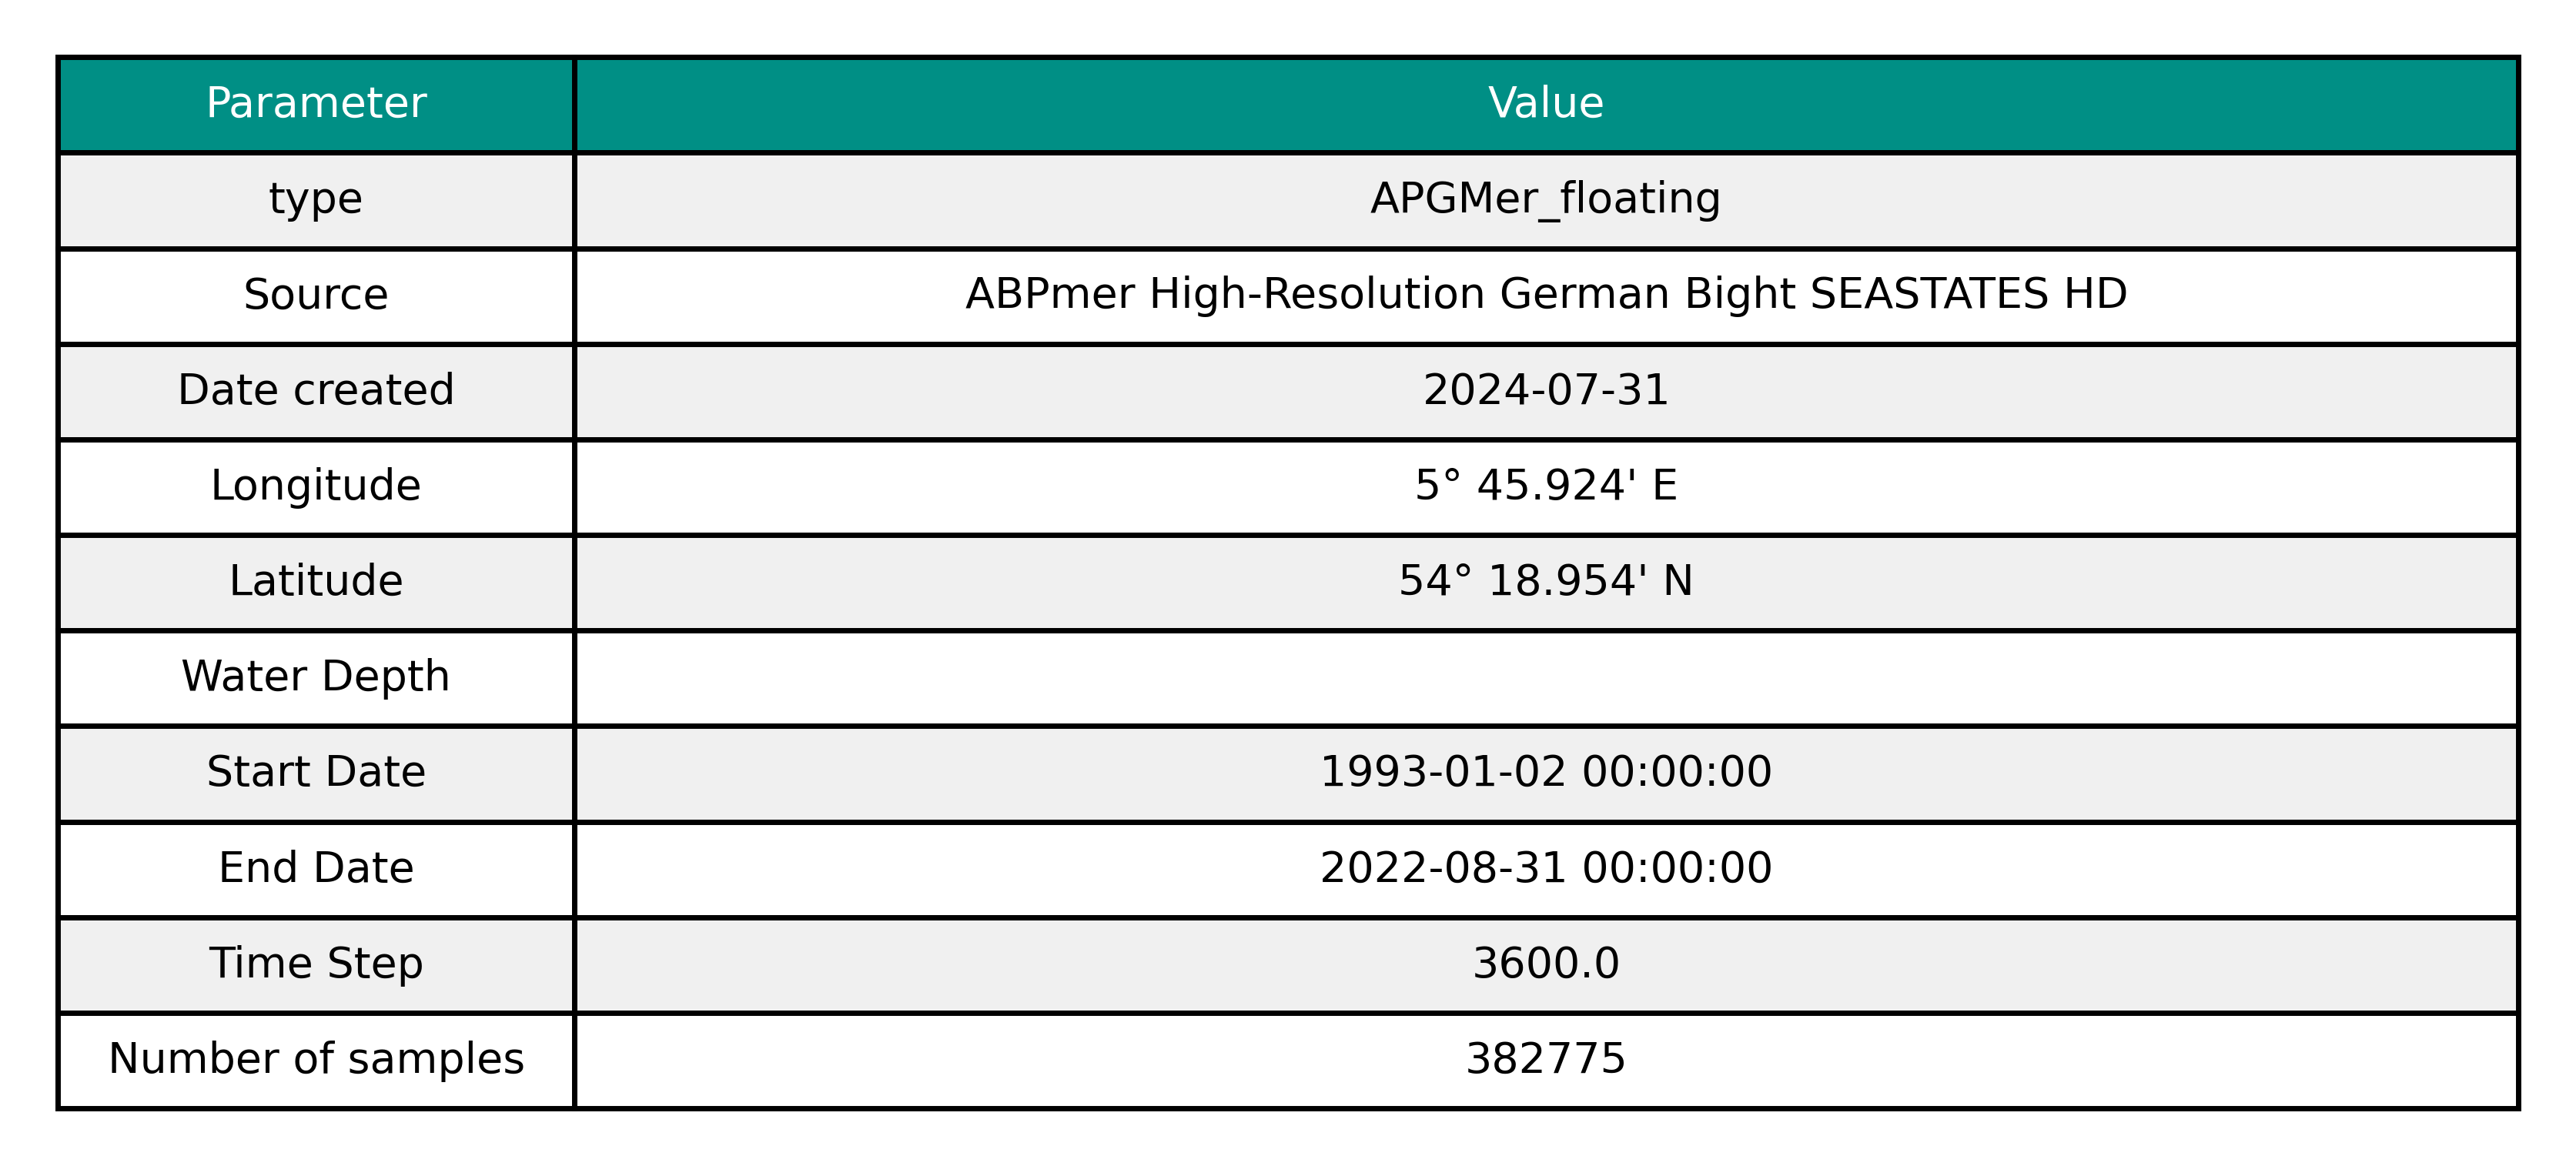
\includegraphics[width=1.0\textwidth ]{C:/Users/aaron.lange/Desktop/Projekte/Hindcast_Tool/HindTool/example_output/DataSorce_Currents_page_1.png} 
 \captionsetup{type=table} 
\caption{ DataSorce-Currents-page-1 } 
 \label{tab: DataSorce_Currents_page_1 } 
\end{figure}
\begin{figure}[H] 
 \centering 
 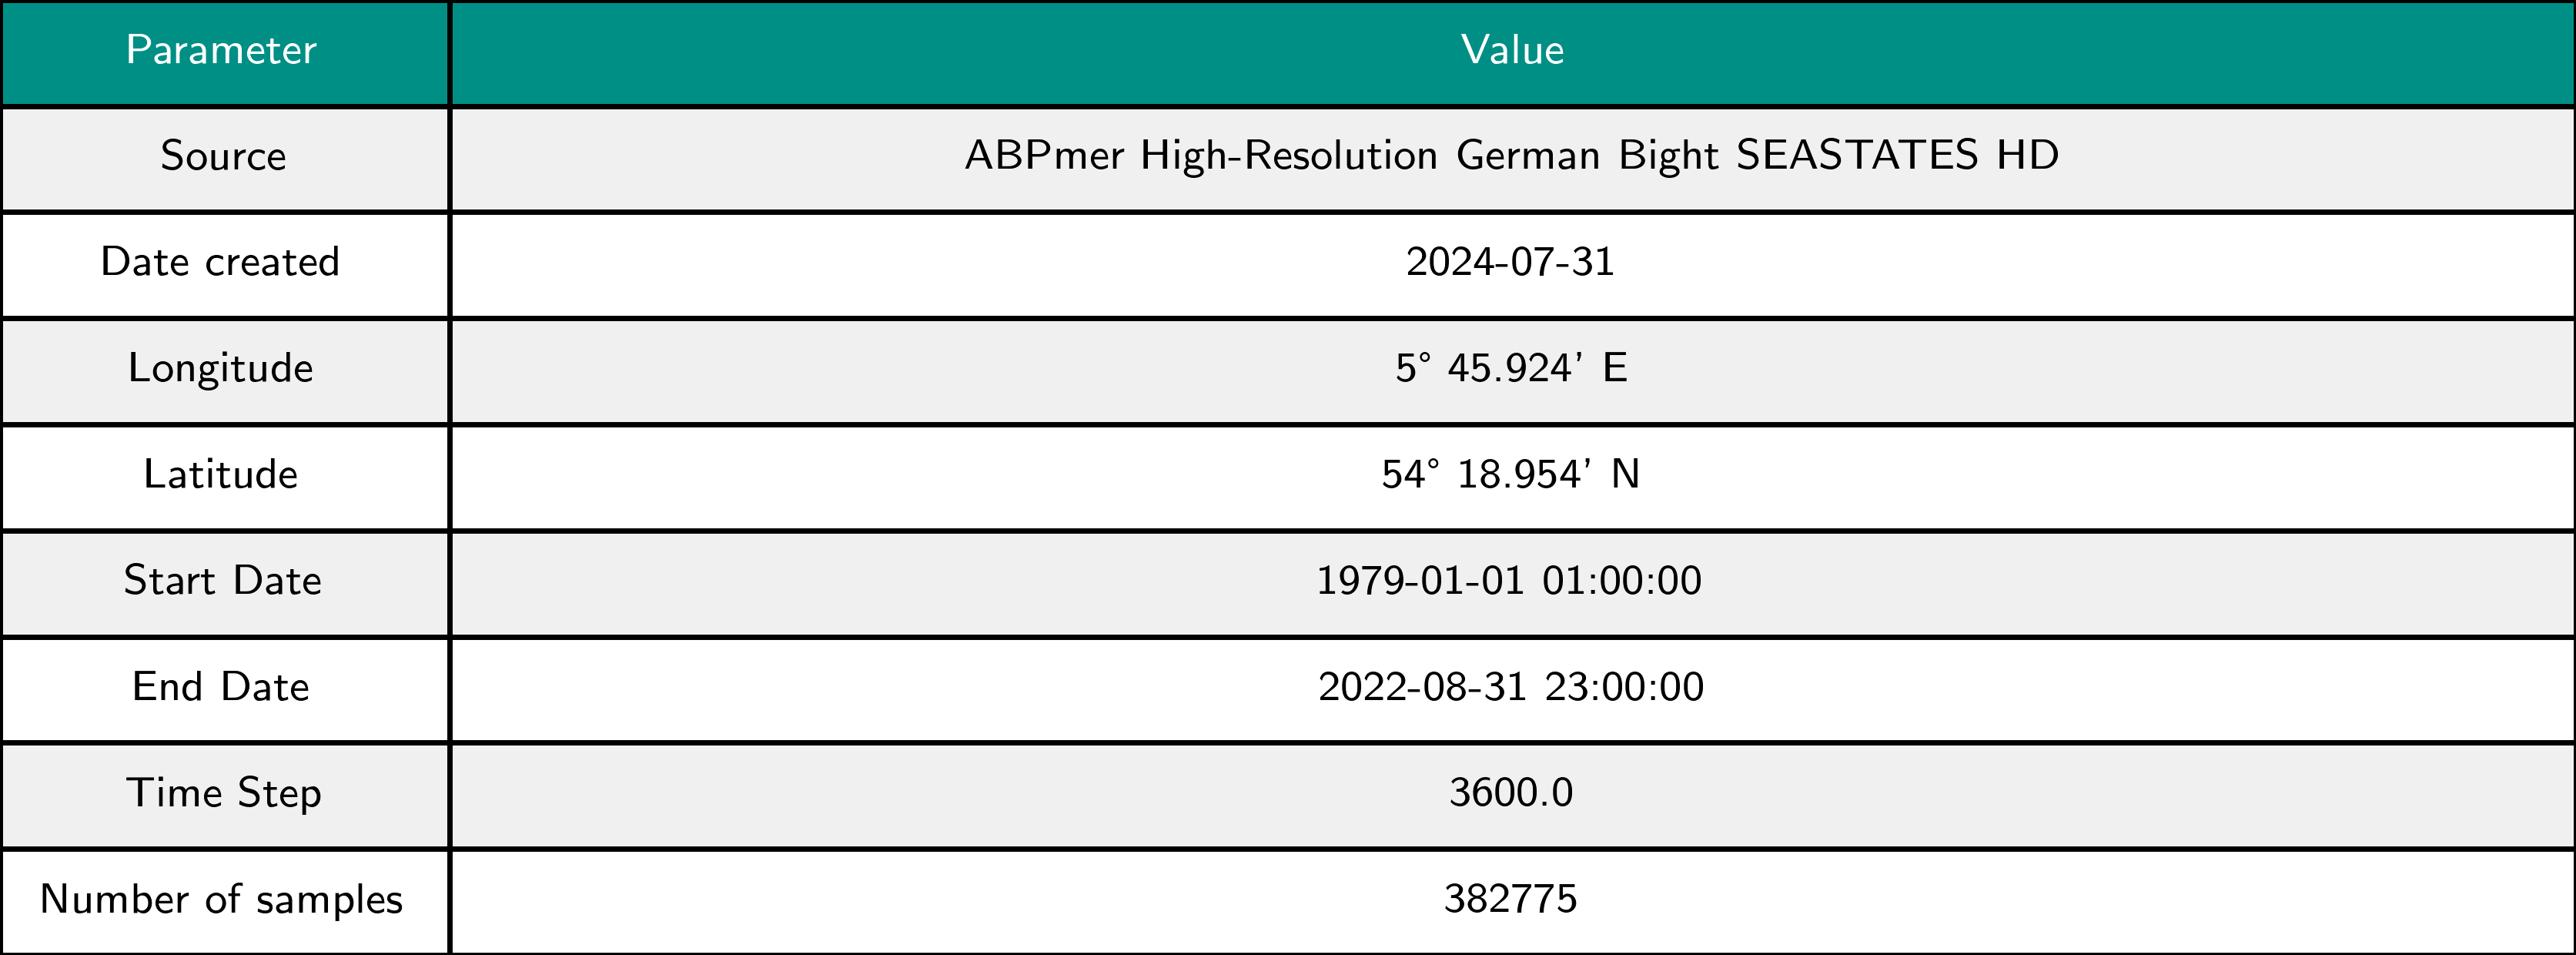
\includegraphics[width=1.0\textwidth ]{C:/Users/aaron.lange/Desktop/Projekte/Hindcast_Tool/HindTool/example_output/DataSorce_Levels_page_1.png} 
 \captionsetup{type=table} 
\caption{ DataSorce-Levels-page-1 } 
 \label{tab: DataSorce_Levels_page_1 } 
\end{figure}
\begin{figure}[H] 
 \centering 
 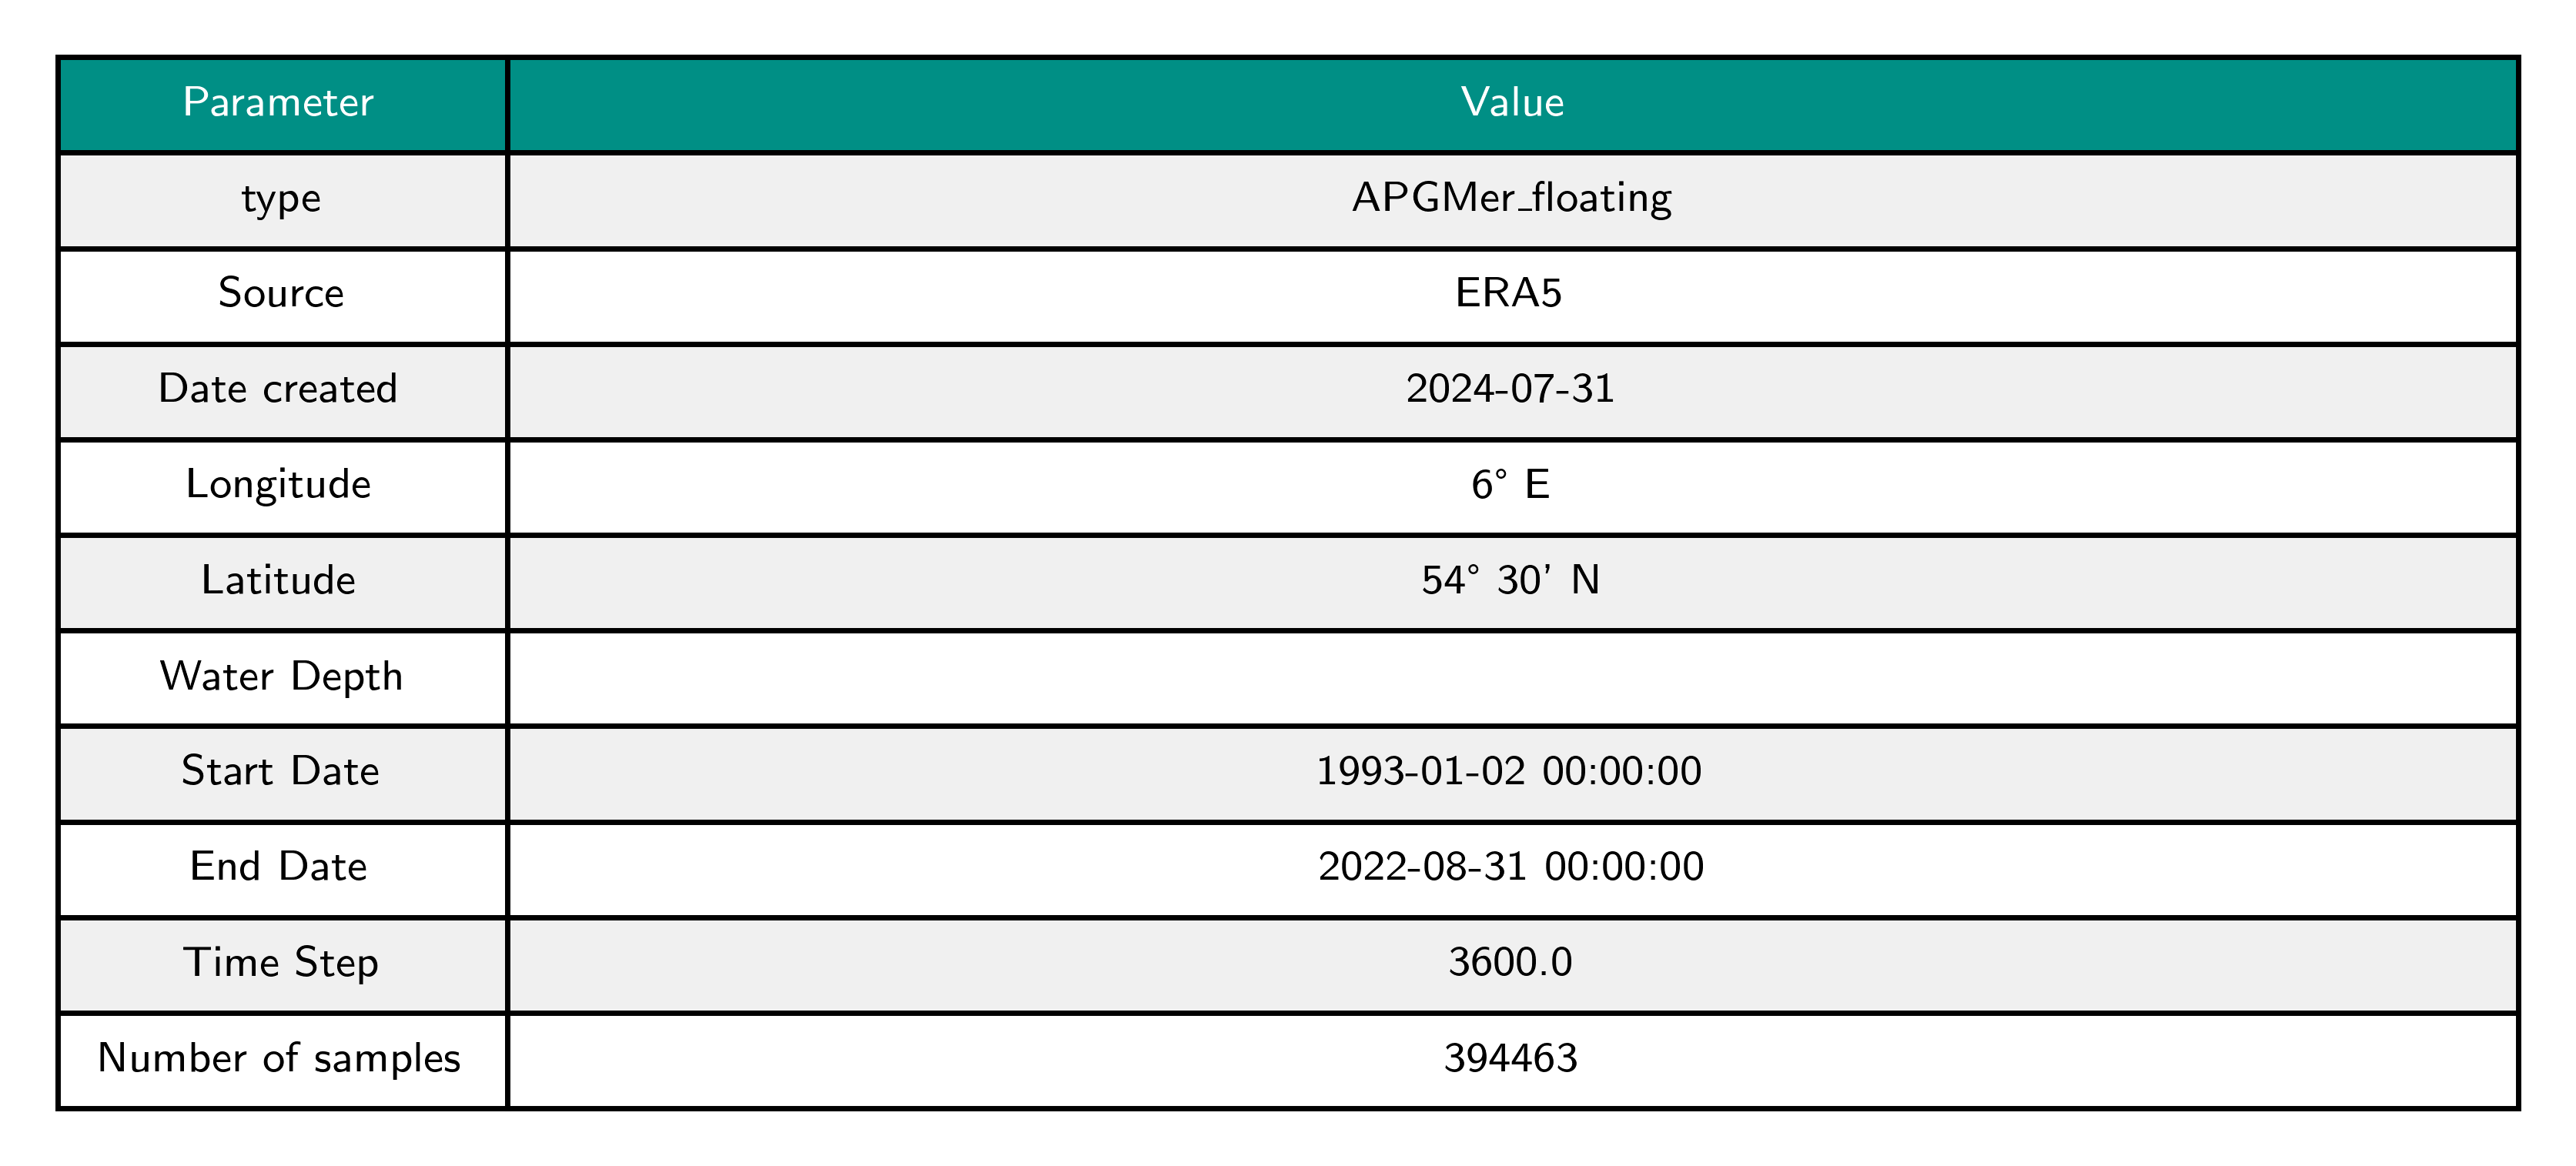
\includegraphics[width=1.0\textwidth ]{C:/Users/aaron.lange/Desktop/Projekte/Hindcast_Tool/HindTool/example_output/DataSorce_Waves_page_1.png} 
 \captionsetup{type=table} 
\caption{ DataSorce-Waves-page-1 } 
 \label{tab: DataSorce_Waves_page_1 } 
\end{figure}
\begin{figure}[H] 
 \centering 
 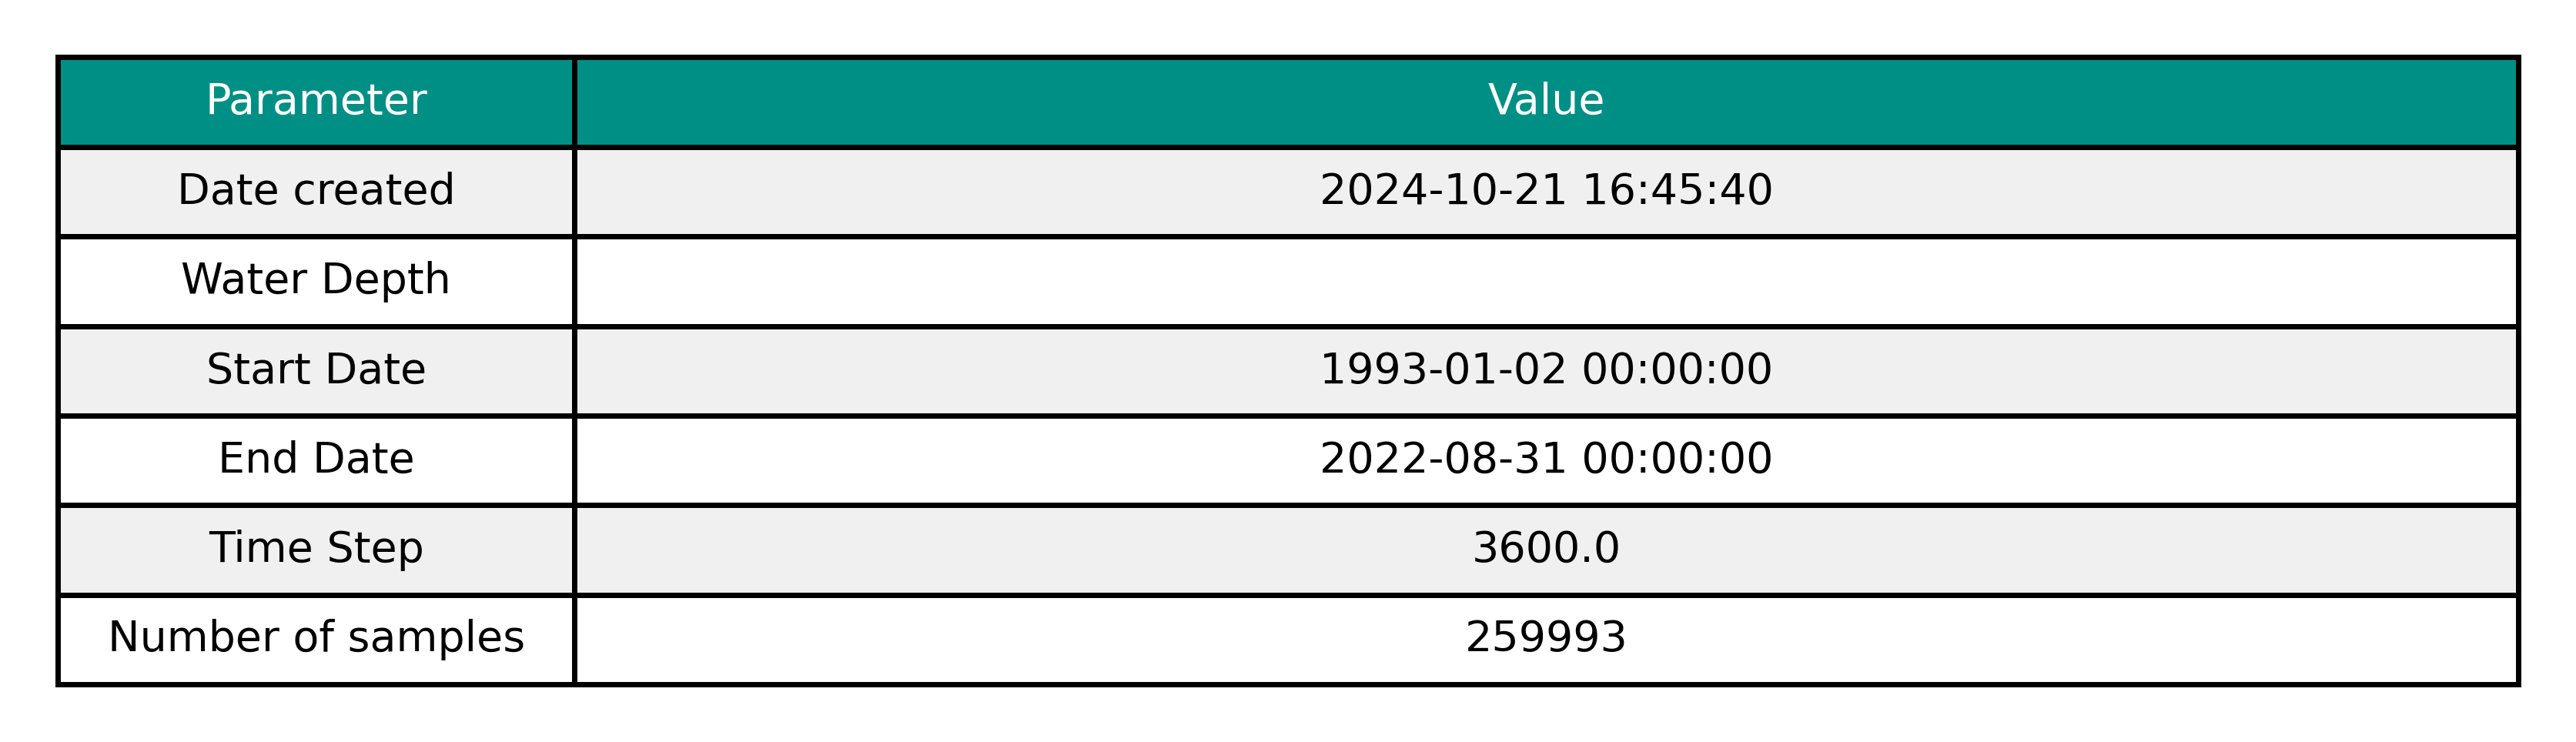
\includegraphics[width=1.0\textwidth ]{C:/Users/aaron.lange/Desktop/Projekte/Hindcast_Tool/HindTool/example_output/DataSorce_Winds_page_1.png} 
 \captionsetup{type=table} 
\caption{ DataSorce-Winds-page-1 } 
 \label{tab: DataSorce_Winds_page_1 } 
\end{figure}


\subsection{Data resampling} 
The timestep of 3600.0 s is chosen to be the timestep for all calculation. Deviating timesteps must be sampled down to be combined with the wave data. For this, the mean of all measurements corresponding to one timestep of wave data is used.
If the timeframes of the datasets are different, the timframe containing all data from the different databasis is choosen in the resampling step to keep all data. For the calculations, only the data present in all relevent databasis are loaded.  In the table below the sampling rates and the resulting numbers of samples as well as the timeframes of the original and the combined datasets are listed.

\begin{figure}[H] 
 \centering 
 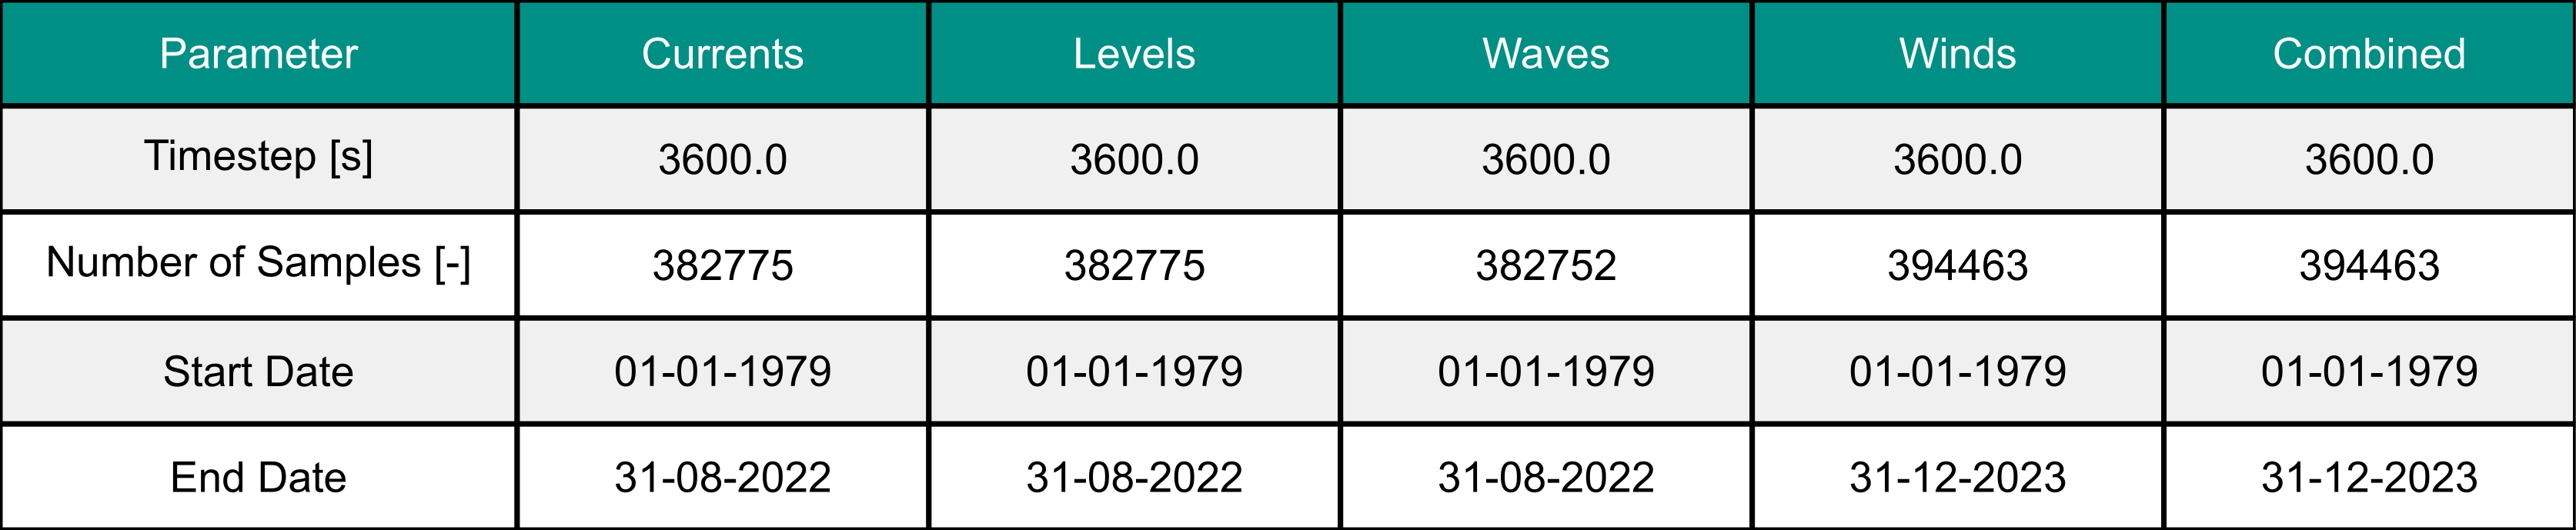
\includegraphics[width=1.0\textwidth ]{C:/Users/aaron.lange/Desktop/Projekte/Hindcast_Tool/HindTool/example_output/DataSorce_ResamplingTable_page_1.png} 
 \captionsetup{type=table} 
\caption{ DataSorce-ResamplingTable-page-1 } 
 \label{tab: DataSorce_ResamplingTable_page_1 } 
\end{figure}

\subsection{Filtering routines}
All rows containing 'nan' values in one of the relevant sensors are excluded from this specific calculation.  
Also, if the separated wind sea component is used extra filtering is necessary in case of the wind-wave missalignment. Because of the separation process of wind sea and swell, some components can be zero if there is no separable wind sea component. In this case, the wave period is zero as well and the wave direction can’t be determined anymore and is set to 0°, which also distorts the angle misalignment evaluations. For this reason, these sea states are excluded. 
\include{GeneralTheorie}
\section{Sensor analysis}
An overview of the applied sensors is provided in REFERNECE. For each sensor the histogram and the global time series is provided in this chapter.

\subsection{Sensor overview}

Investigated sensors are tabulated below:

\begin{figure}[H] 
 \centering 
 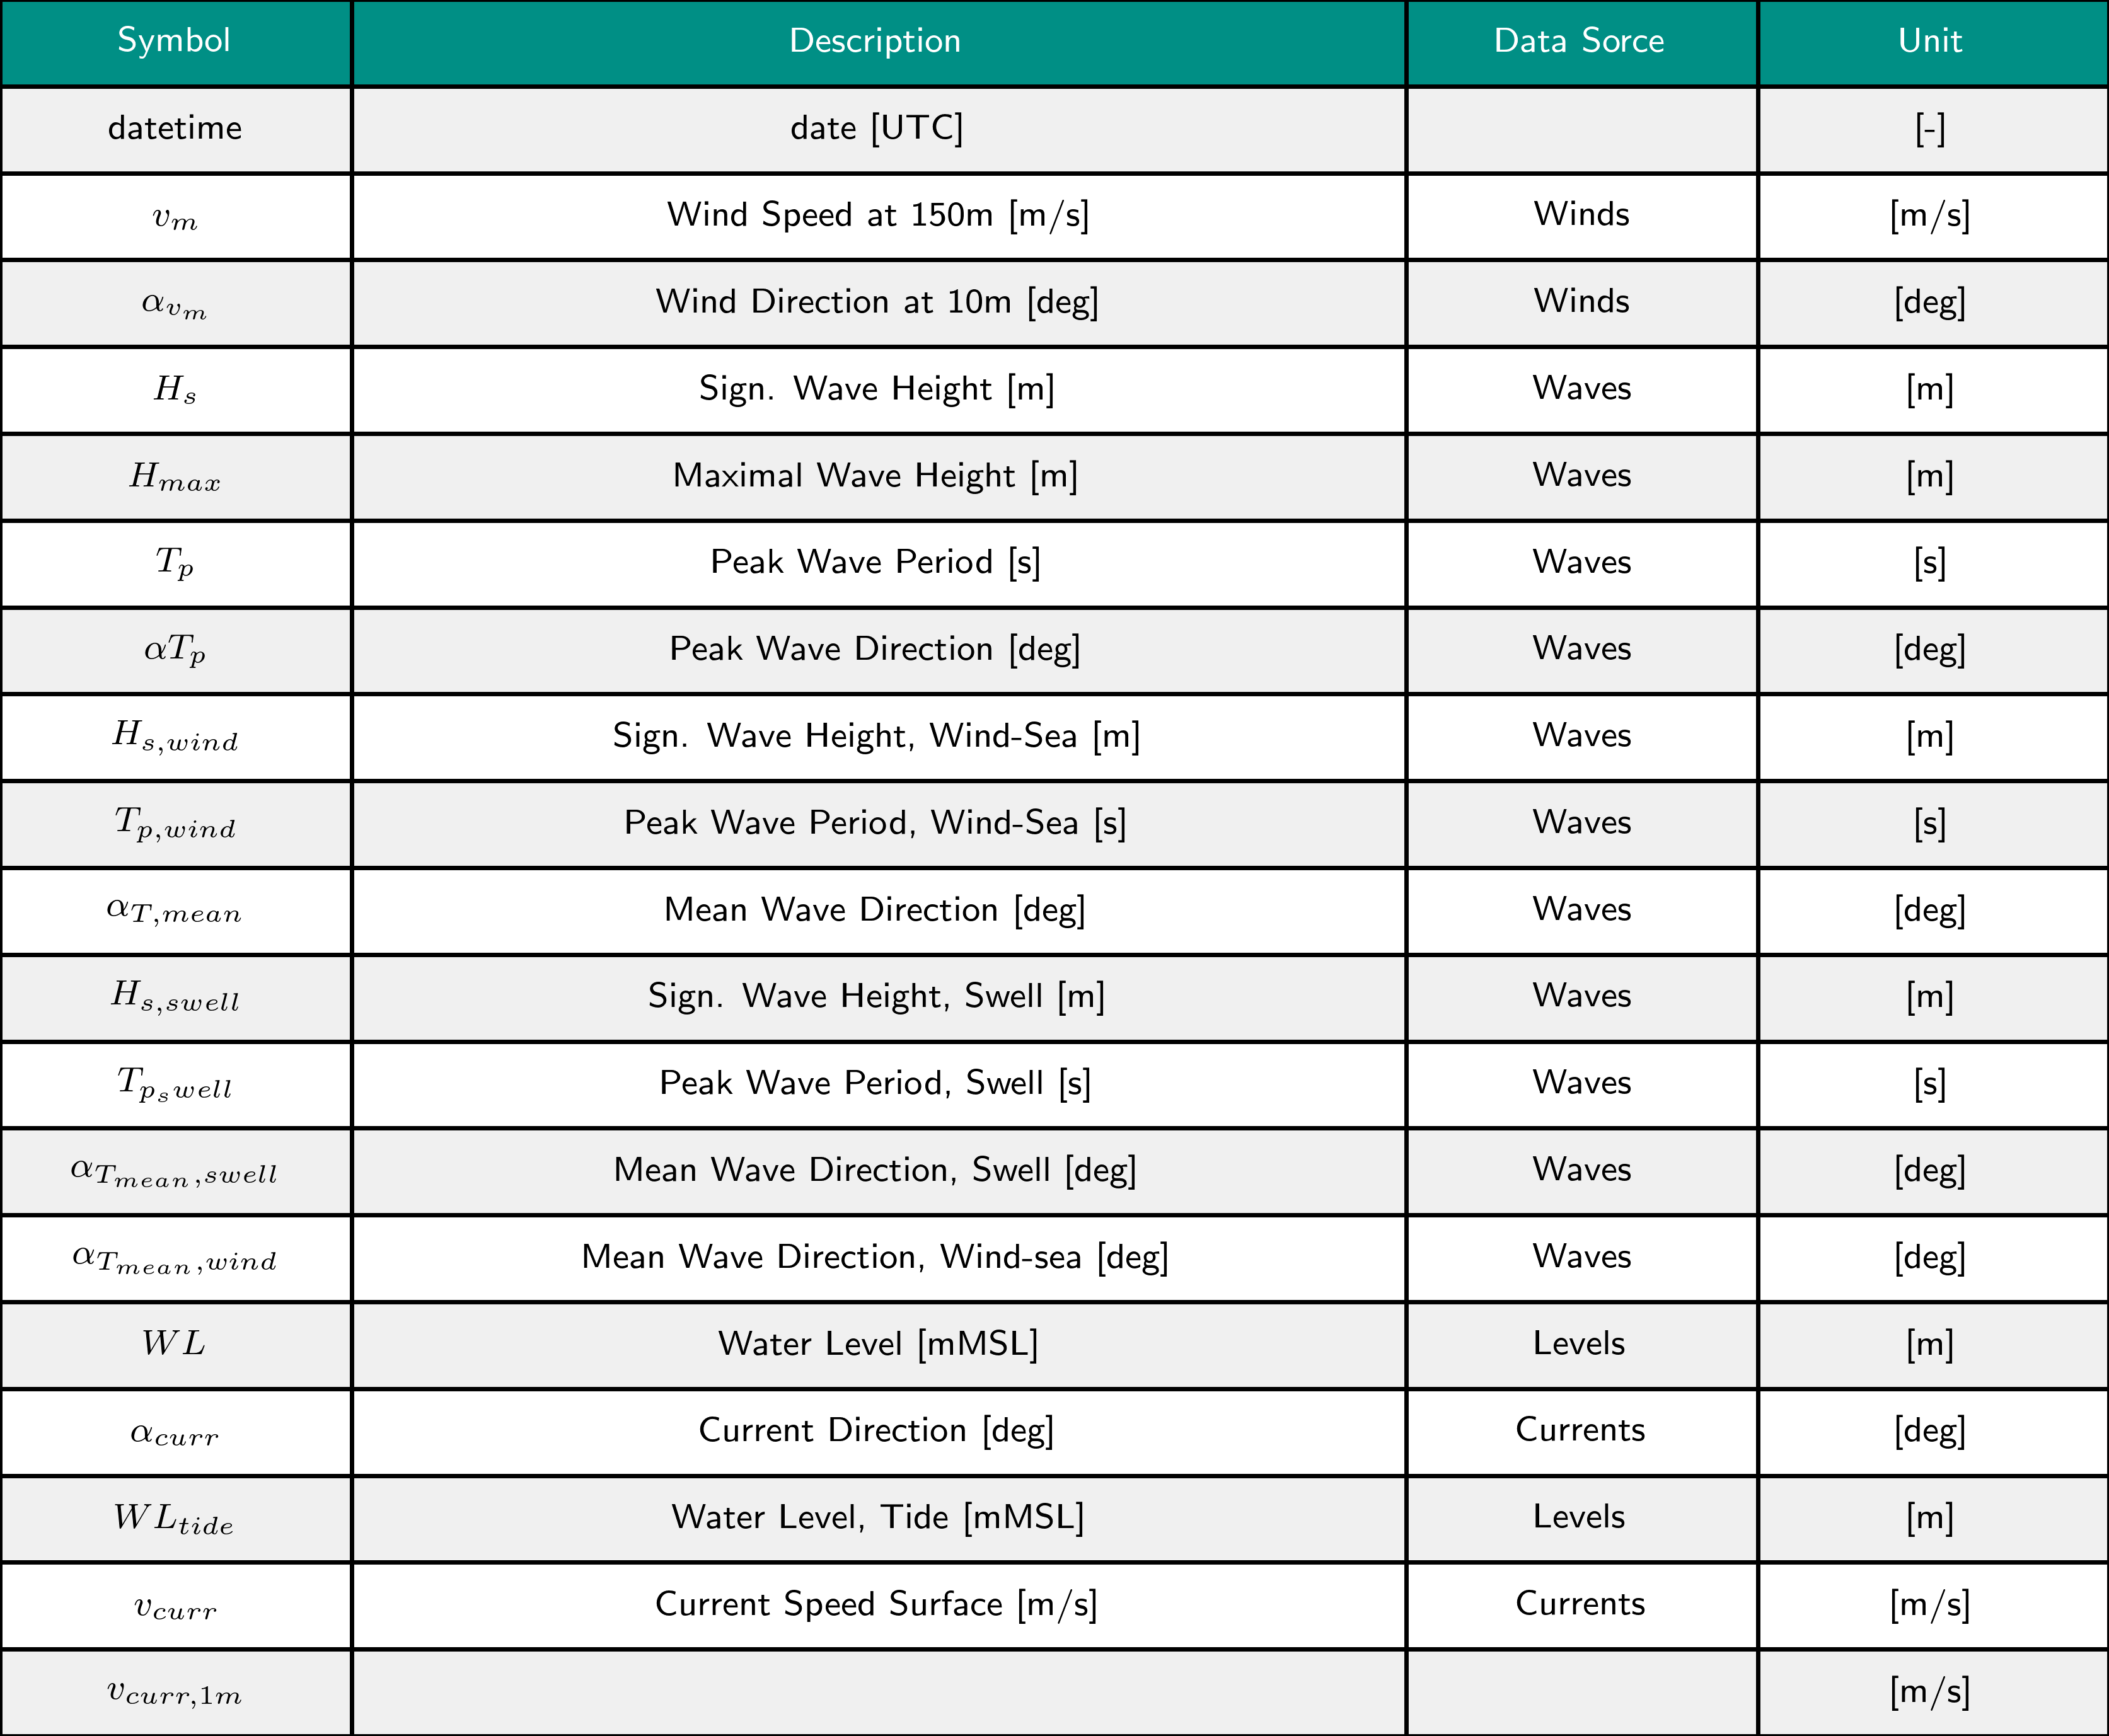
\includegraphics[width=1.0\textwidth ]{C:/Users/aaron.lange/Desktop/Projekte/Hindcast_Tool/HindTool/example_output/Sensor_names_page_1.png} 
 \captionsetup{type=table} 
\caption{ Sensor-names-page-1 } 
 \label{tab: Sensor_names_page_1 } 
\end{figure}

\clearpage 

\subsection{Sensor illustration}

\subsubsection{Sensor: Wind Speed at 150m [m/s]} 
\begin{figure}[H] 
 \centering 
 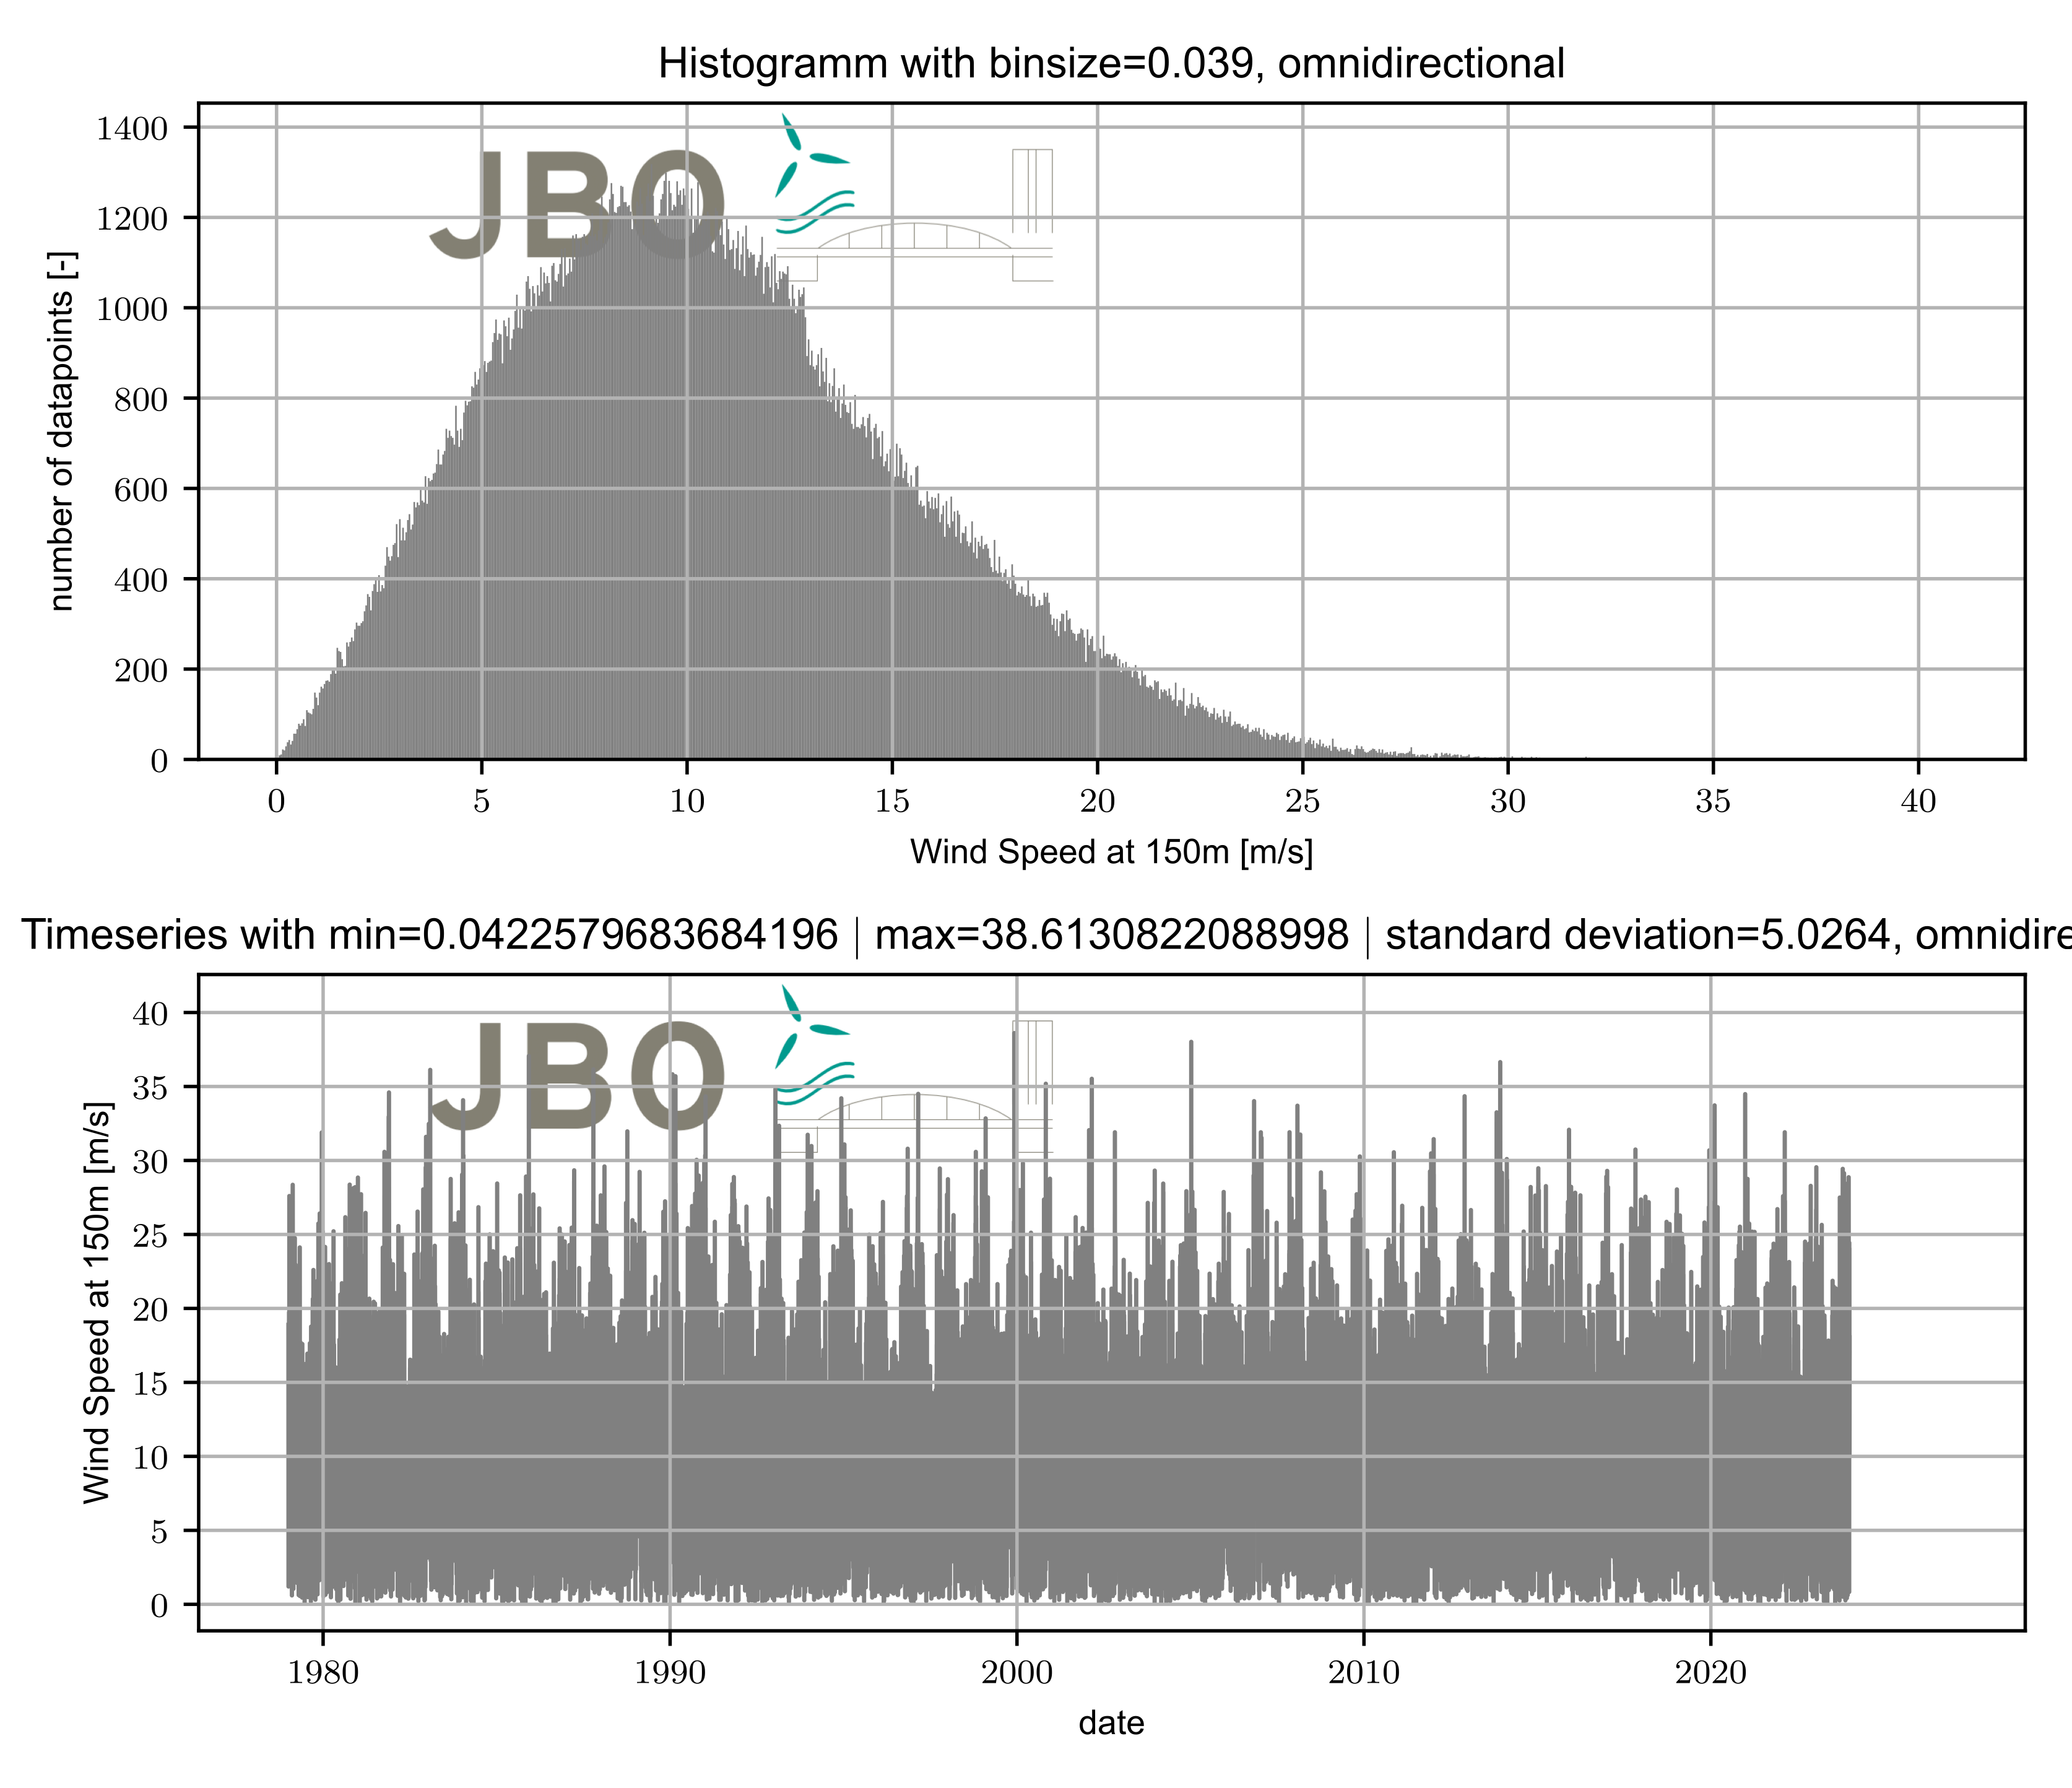
\includegraphics[width=1.0\textwidth]{C:/Users/aaron.lange/Desktop/Projekte/Hindcast_Tool/HindTool/example_output/SensorEval_v_m_page_1.png} 
 \caption{ Timeseries and Histogram of Sensor: Wind Speed at 150m [m/s] } 
 \label{fig: SensorEval_v_m_page_1 } 
\end{figure}
 \clearpage
\subsubsection{Sensor: Sign. Wave Height [m]} 
\begin{figure}[H] 
 \centering 
 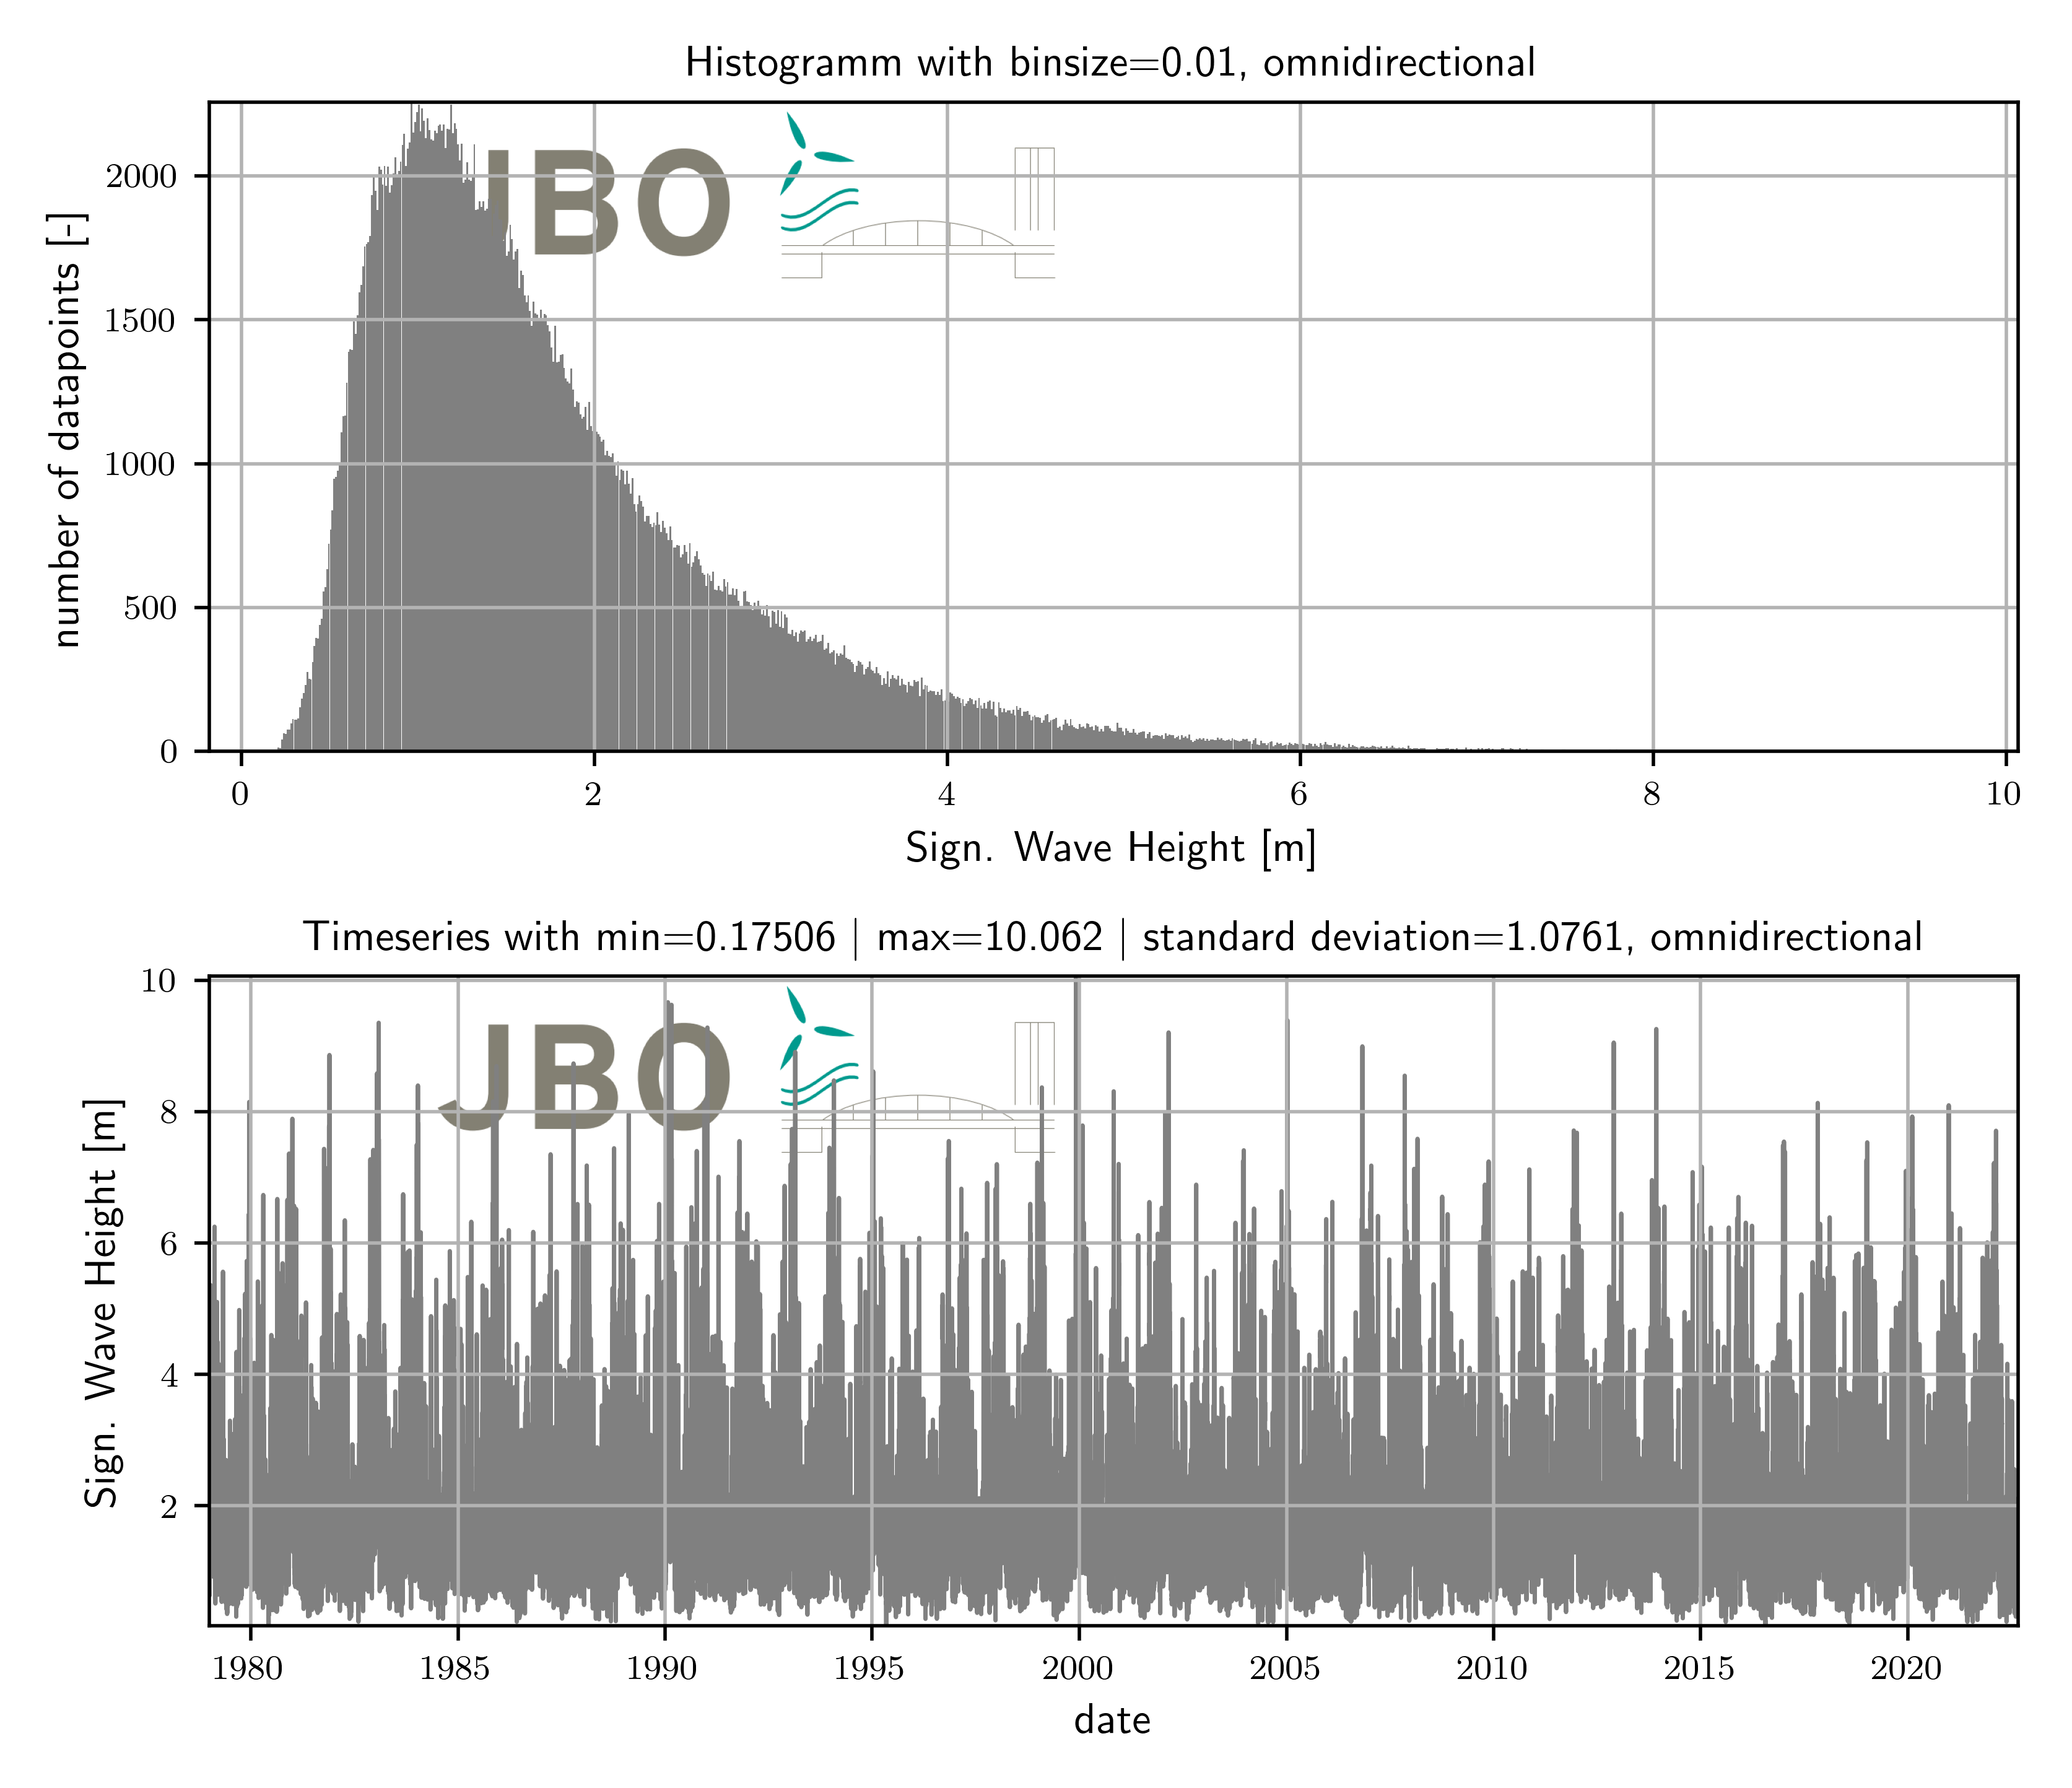
\includegraphics[width=1.0\textwidth]{C:/Users/aaron.lange/Desktop/Projekte/Hindcast_Tool/HindTool/example_output/SensorEval_H_s_page_1.png} 
 \caption{ Timeseries and Histogram of Sensor: Sign. Wave Height [m] } 
 \label{fig: SensorEval_H_s_page_1 } 
\end{figure}
 \clearpage
\subsubsection{Sensor: Maximal Wave Height [m]} 
\begin{figure}[H] 
 \centering 
 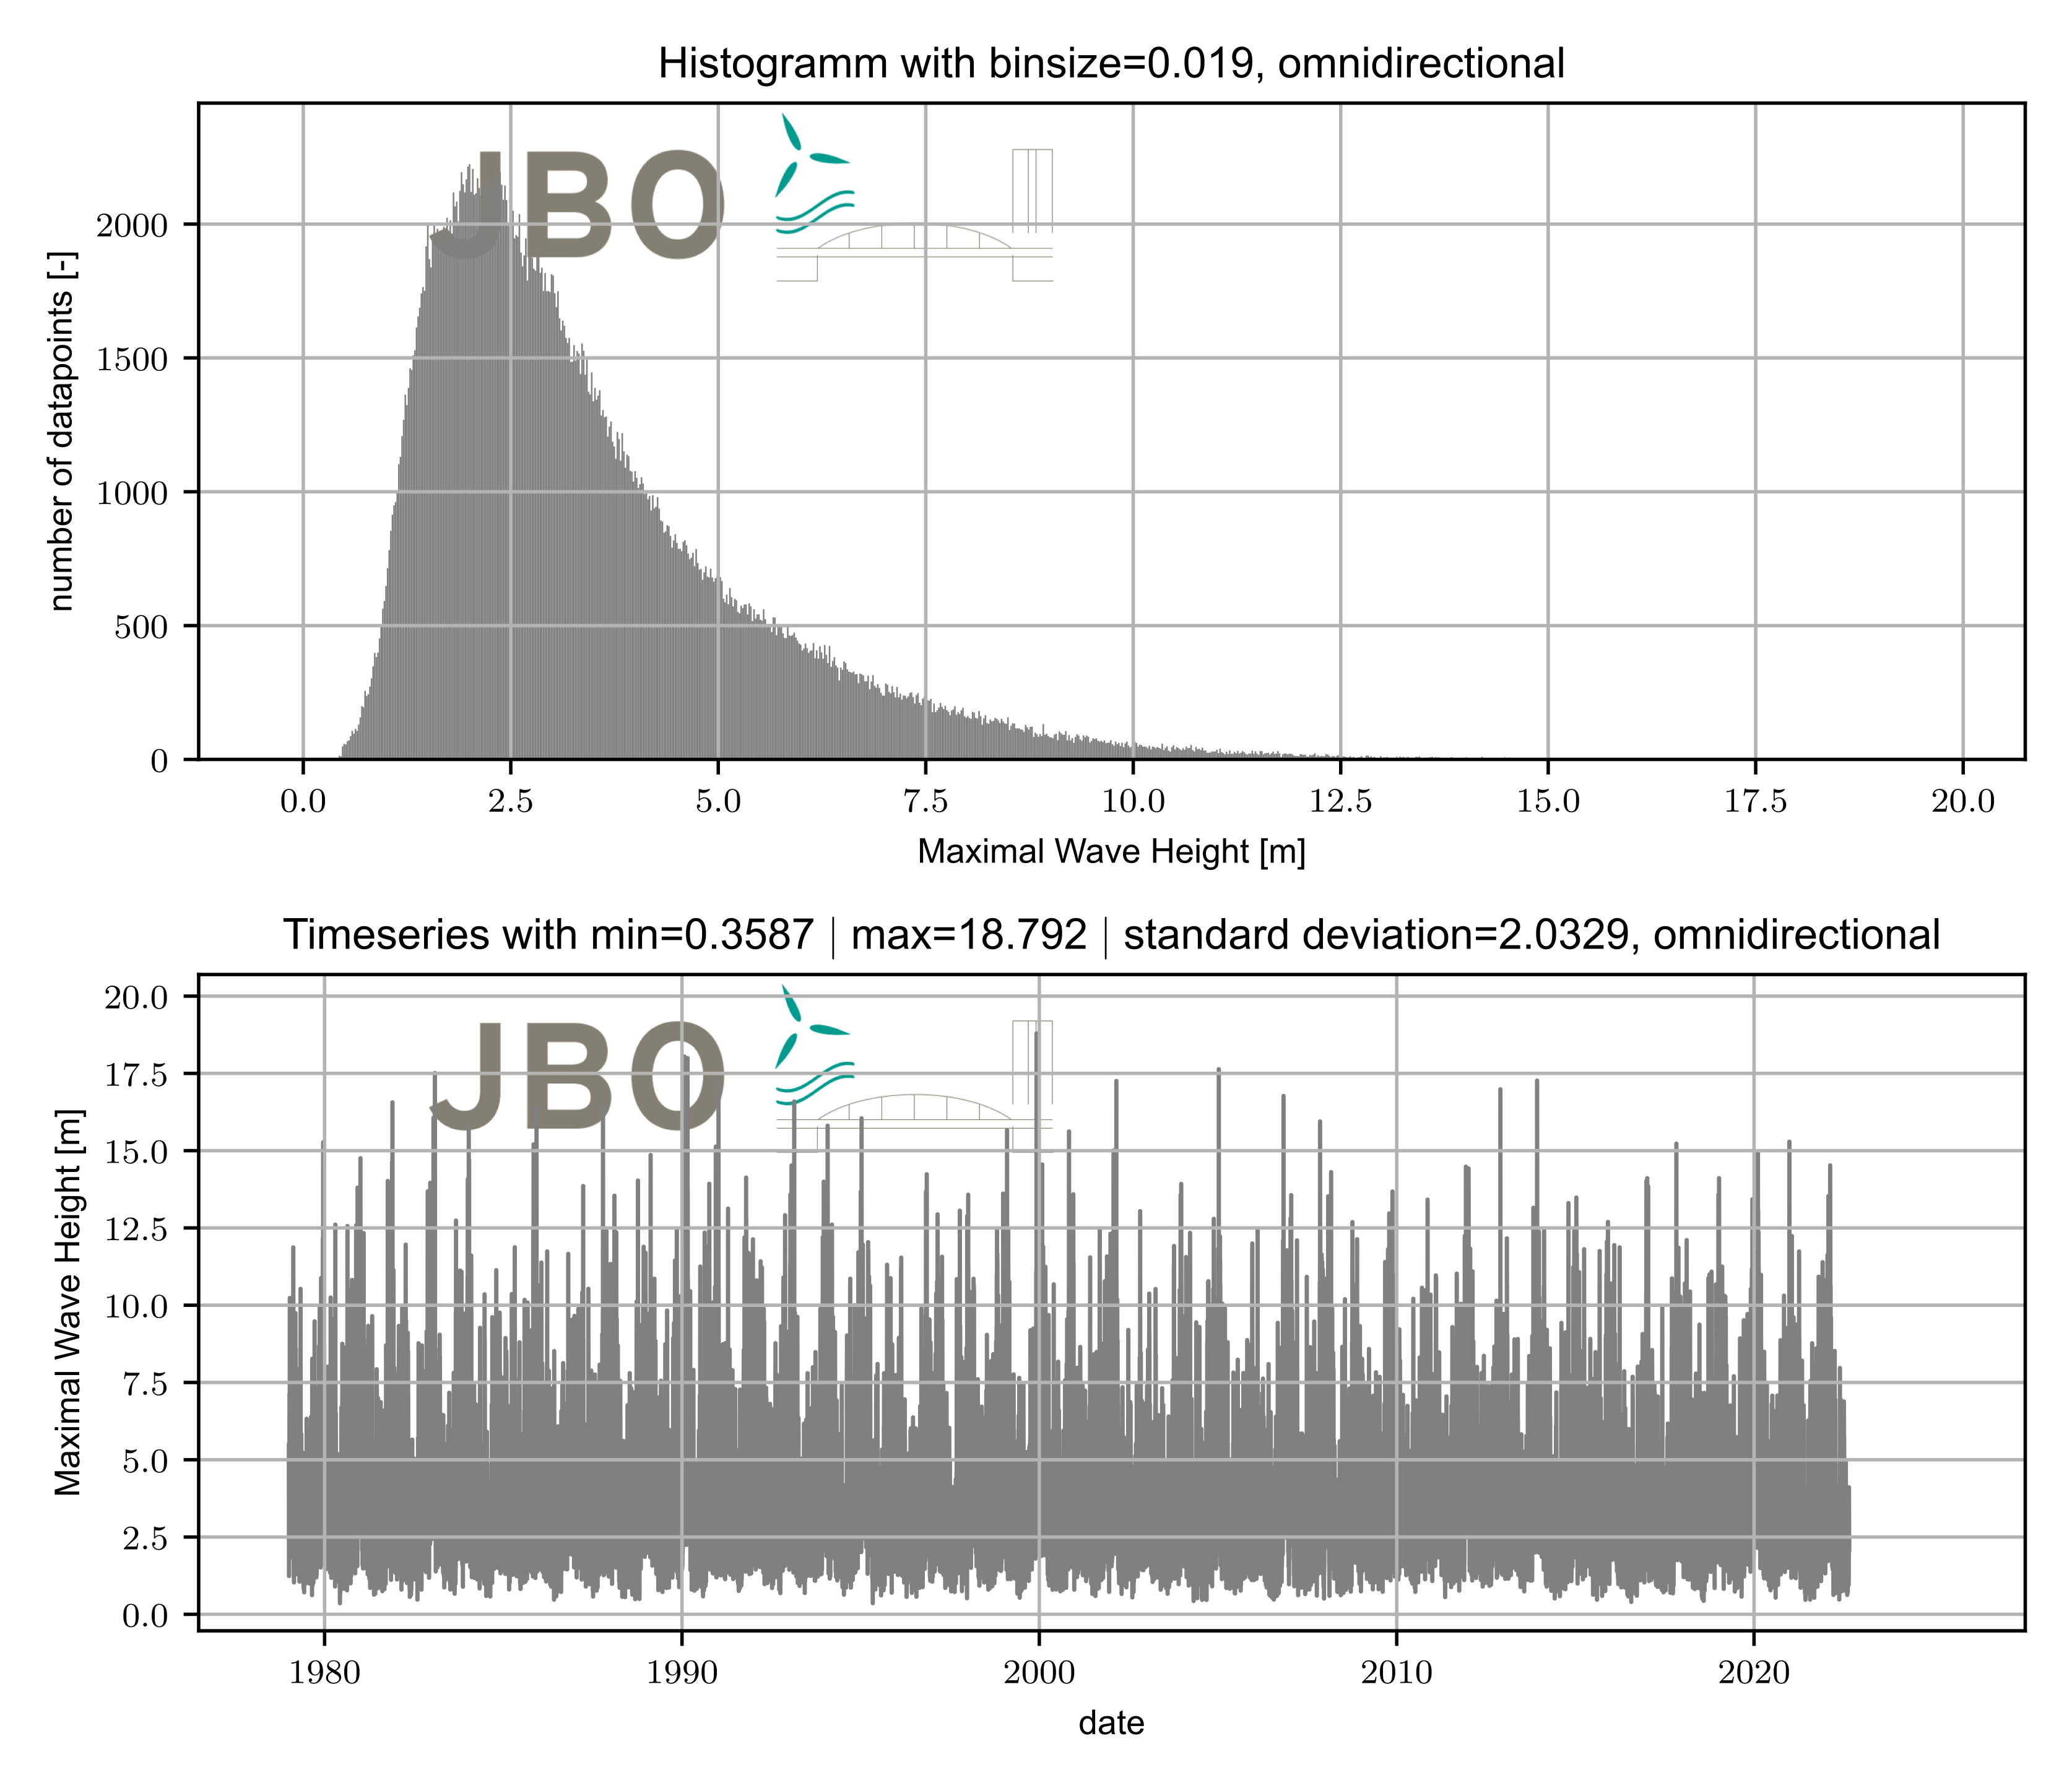
\includegraphics[width=1.0\textwidth]{C:/Users/aaron.lange/Desktop/Projekte/Hindcast_Tool/HindTool/example_output/SensorEval_H_max_page_1.png} 
 \caption{ Timeseries and Histogram of Sensor: Maximal Wave Height [m] } 
 \label{fig: SensorEval_H_max_page_1 } 
\end{figure}
 \clearpage
\subsubsection{Sensor: Peak Wave Period [s]} 
\begin{figure}[H] 
 \centering 
 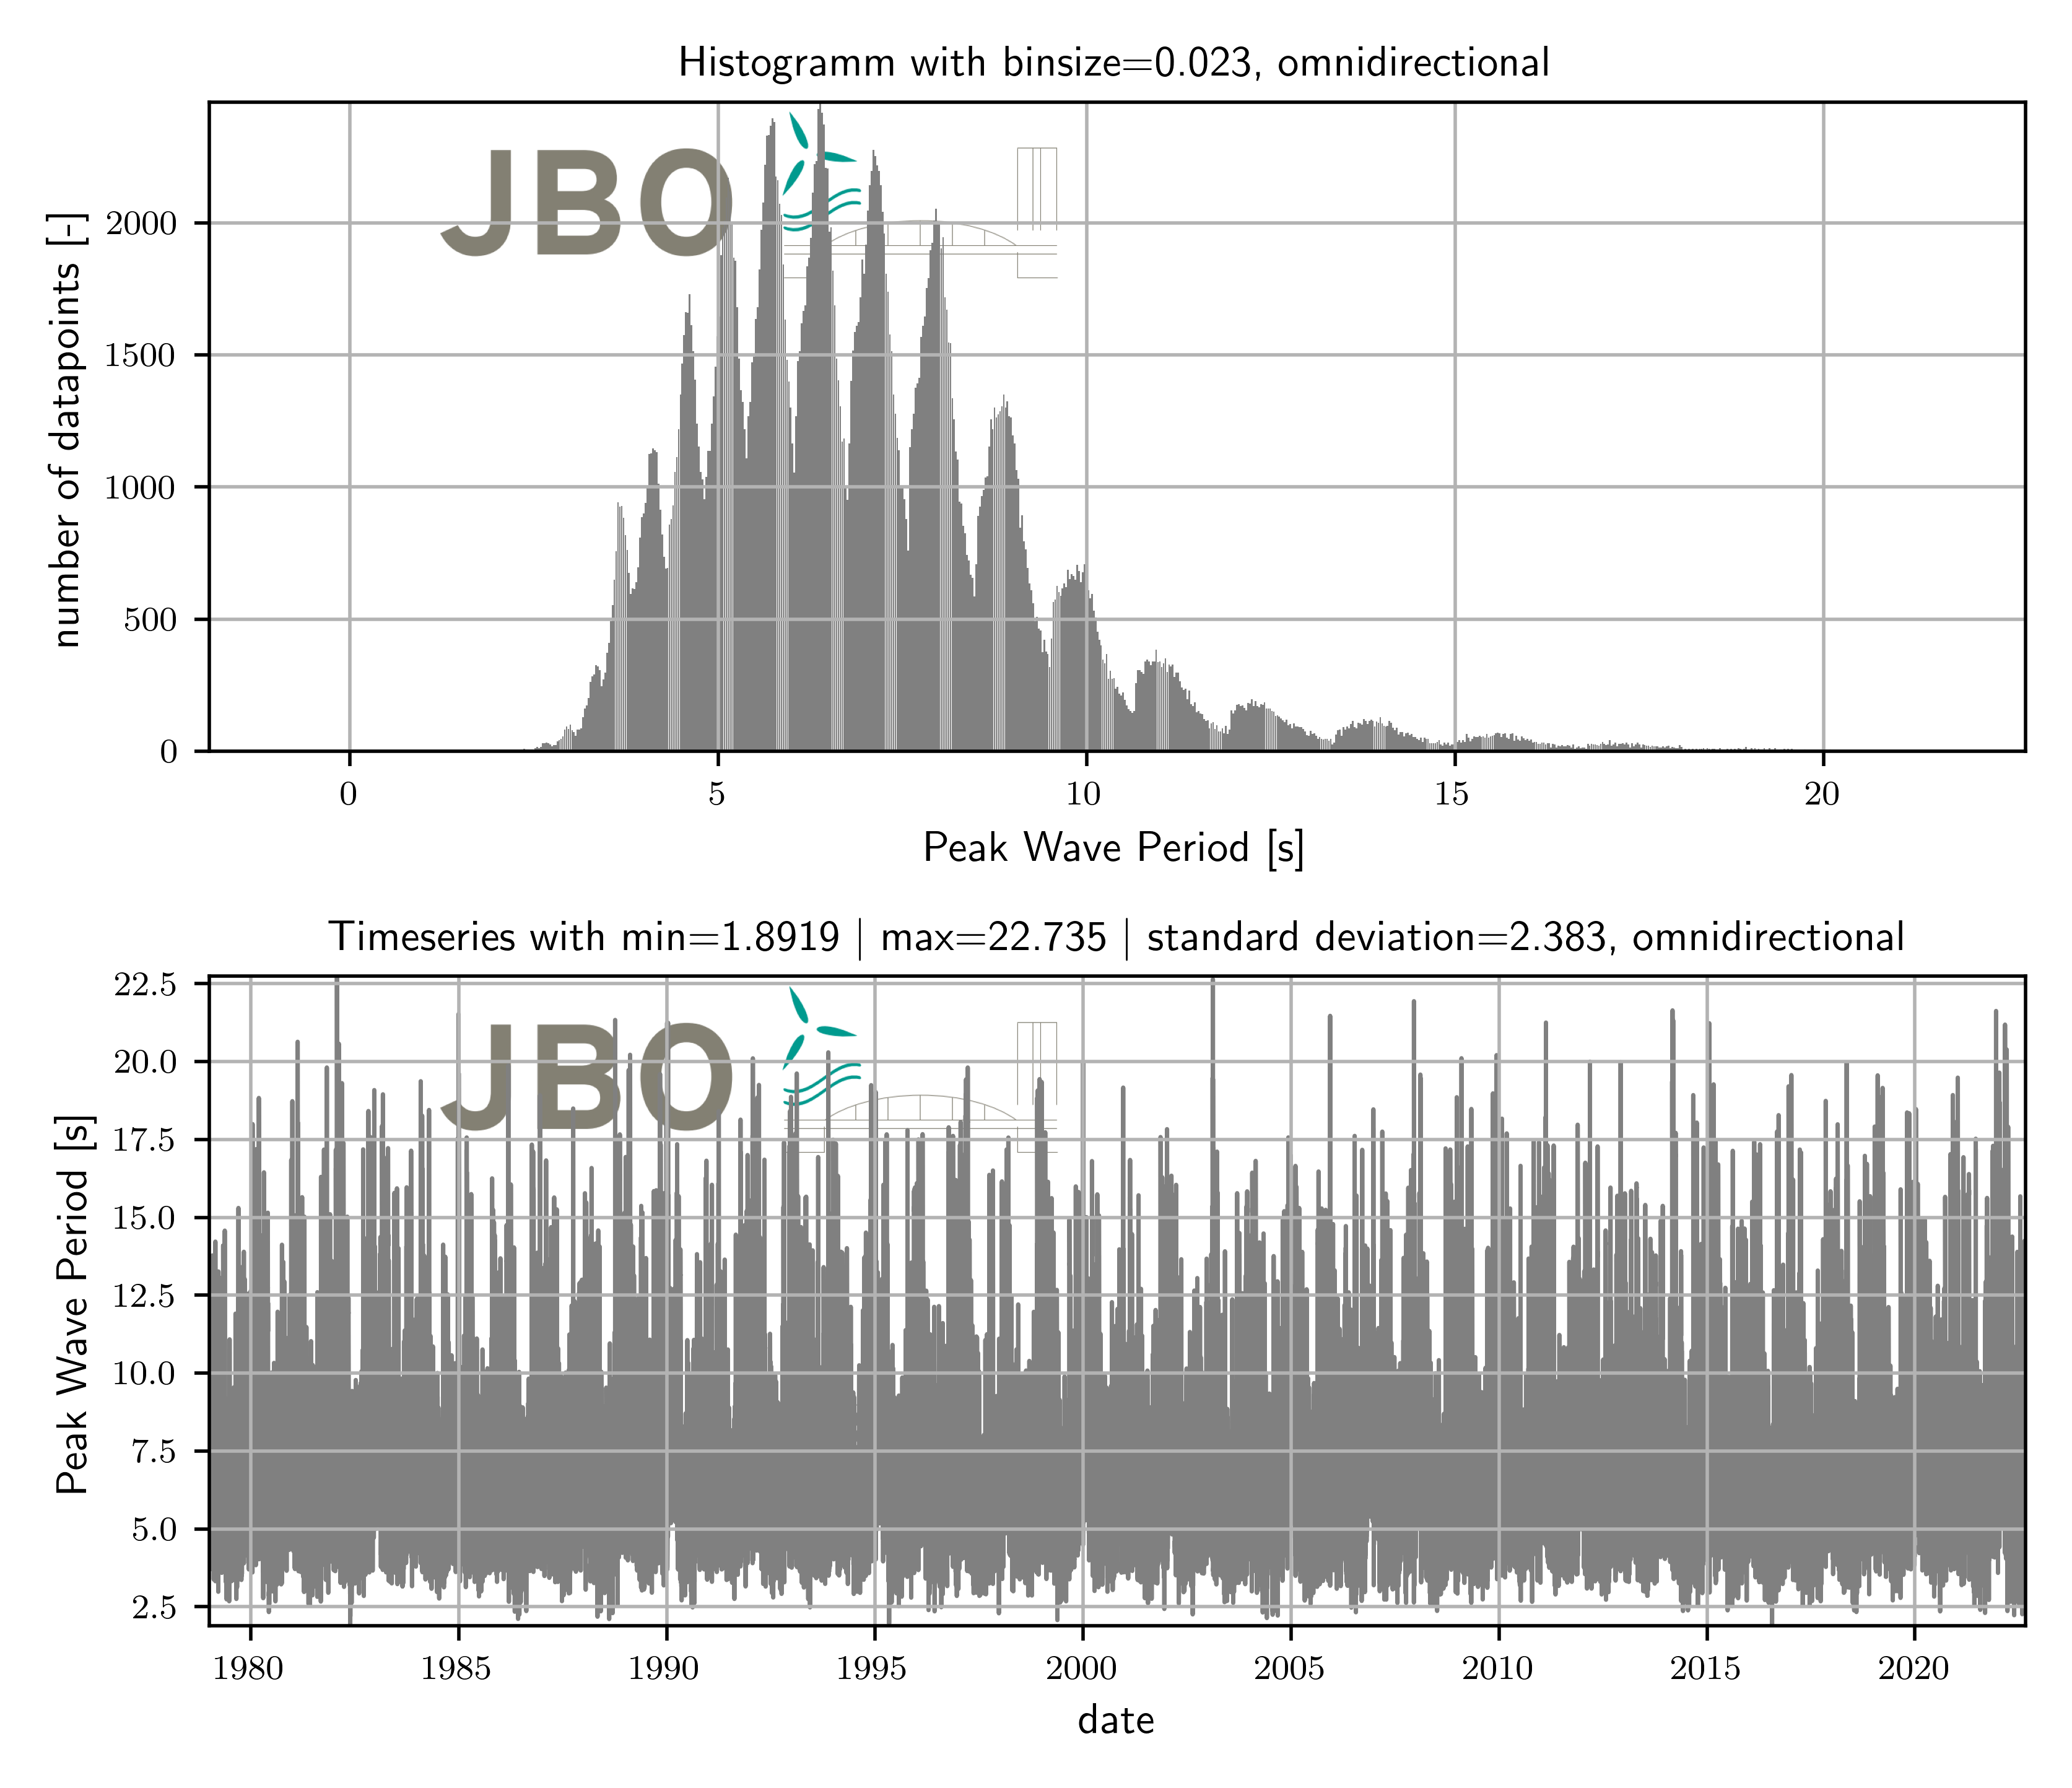
\includegraphics[width=1.0\textwidth]{C:/Users/aaron.lange/Desktop/Projekte/Hindcast_Tool/HindTool/example_output/SensorEval_T_p_page_1.png} 
 \caption{ Timeseries and Histogram of Sensor: Peak Wave Period [s] } 
 \label{fig: SensorEval_T_p_page_1 } 
\end{figure}
 \clearpage
\subsubsection{Sensor: Sign. Wave Height, Wind-Sea [m]} 
\begin{figure}[H] 
 \centering 
 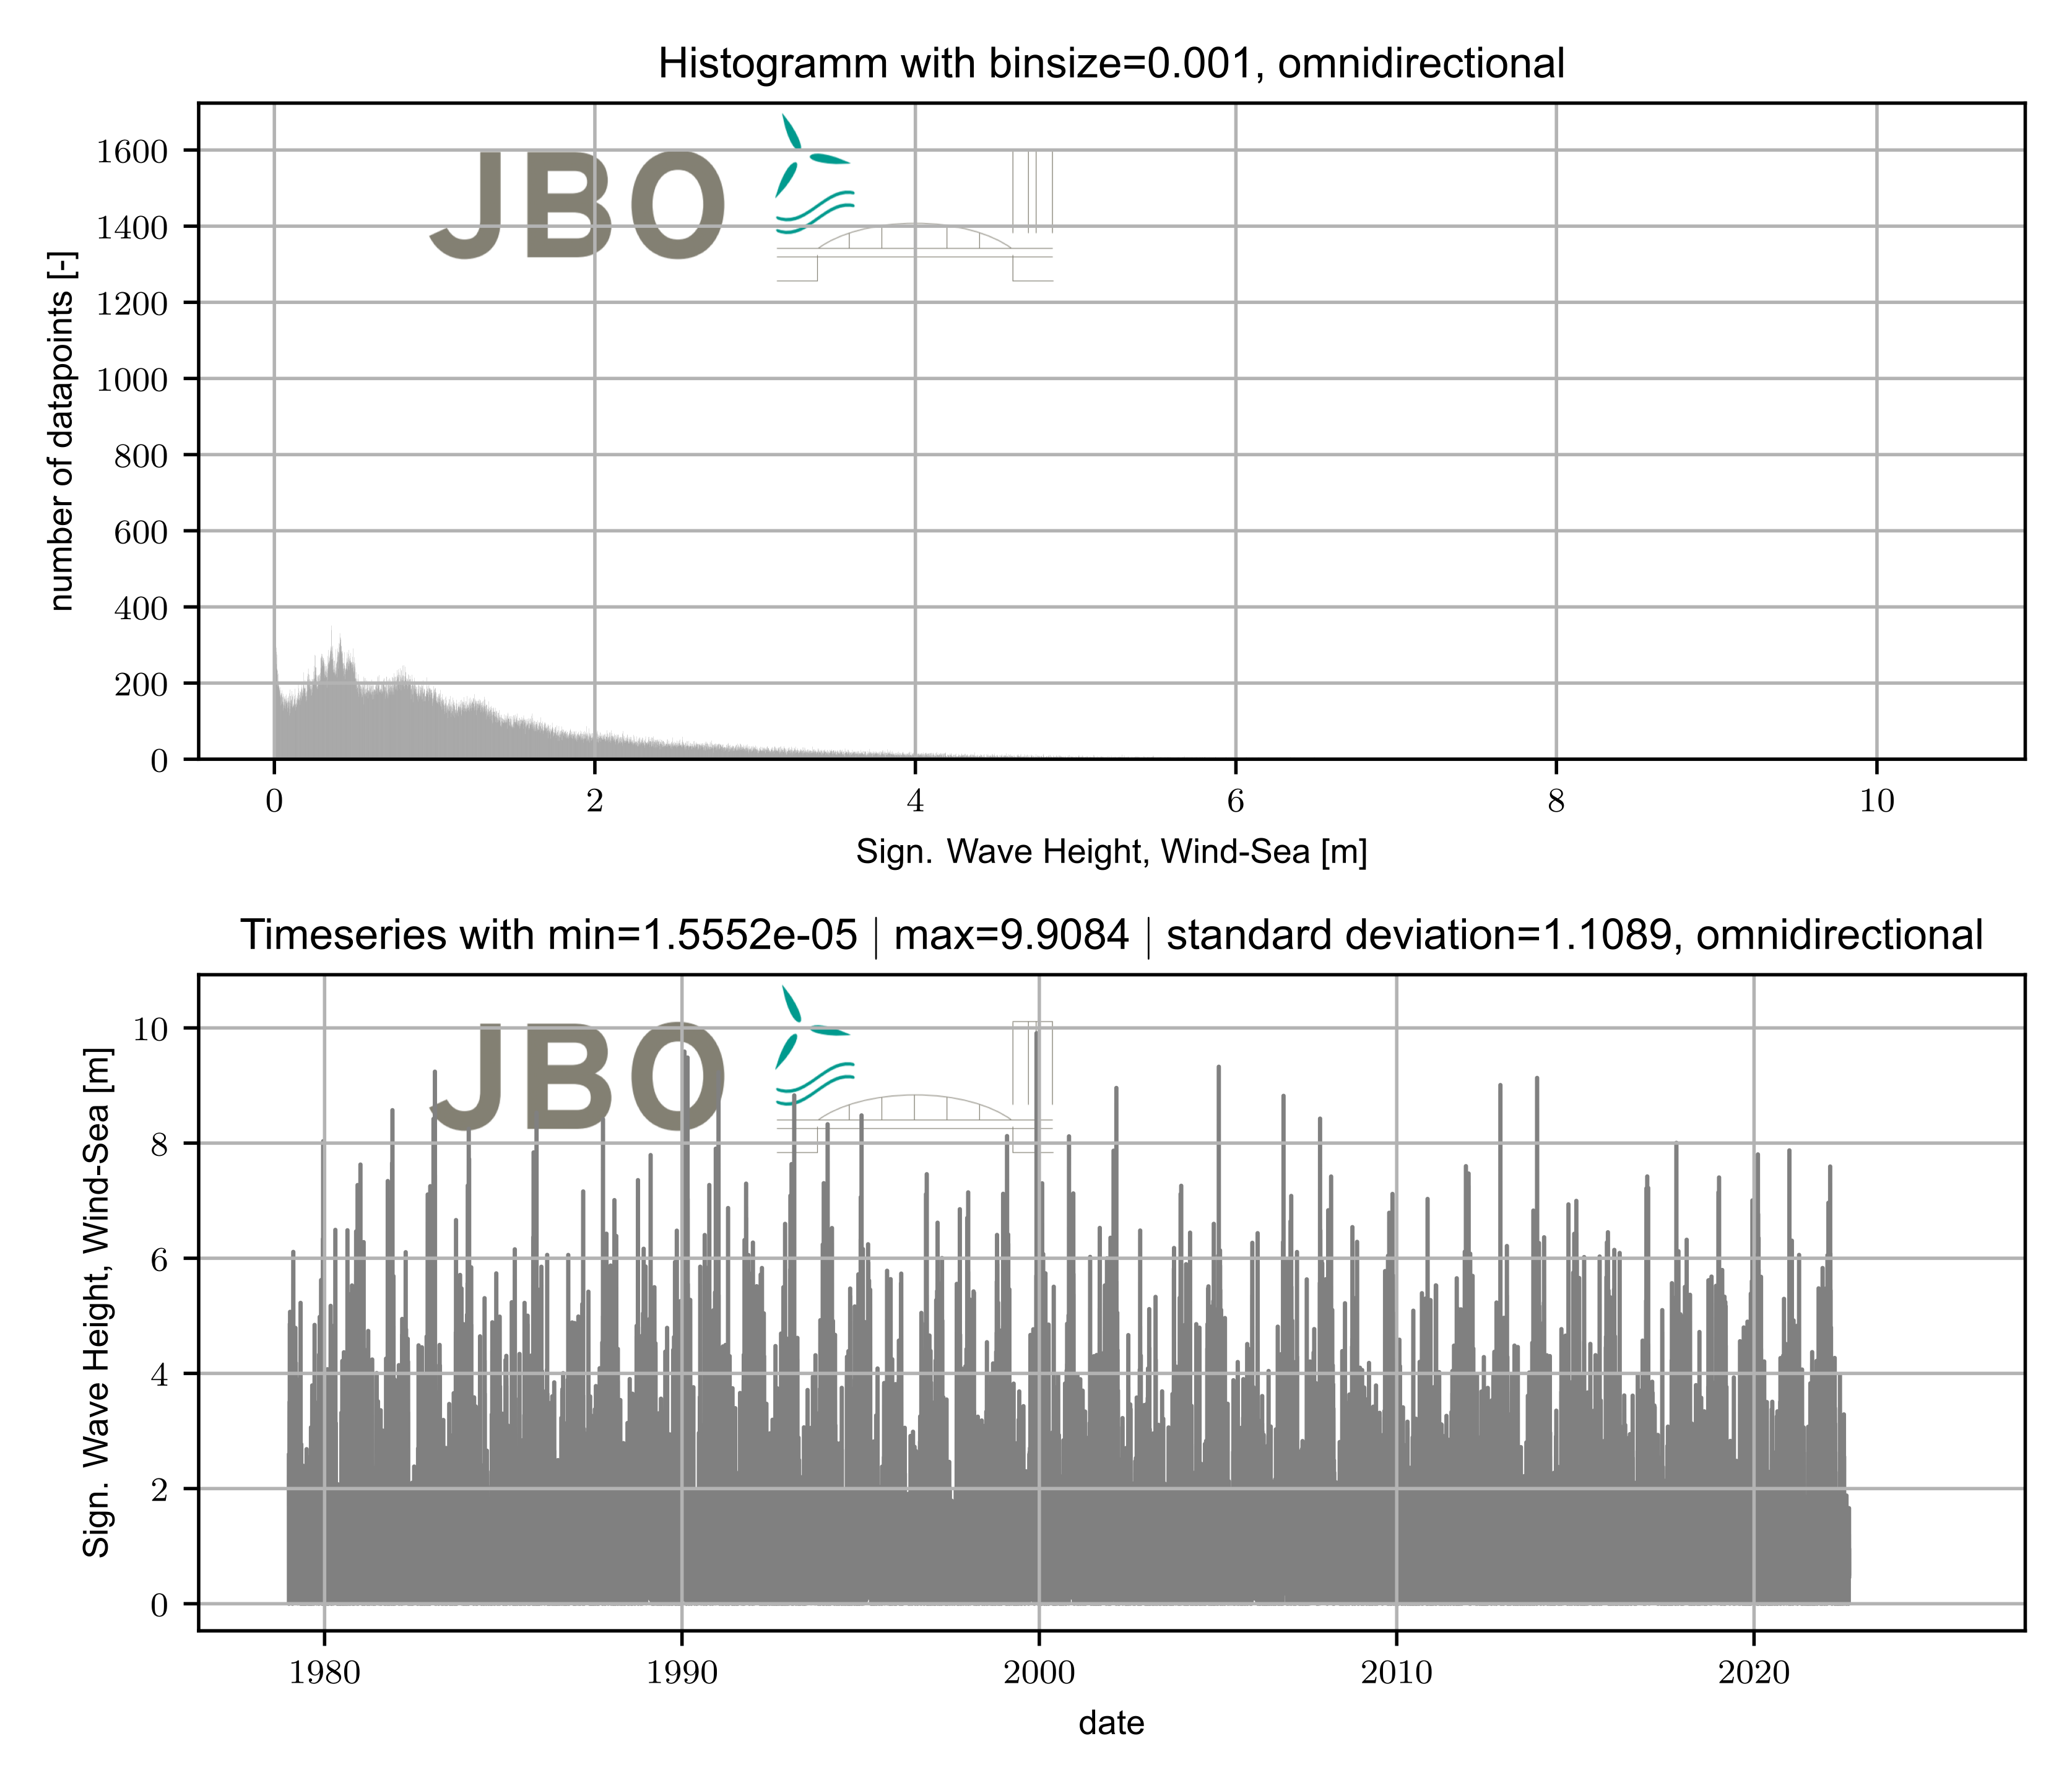
\includegraphics[width=1.0\textwidth]{C:/Users/aaron.lange/Desktop/Projekte/Hindcast_Tool/HindTool/example_output/SensorEval_H_s_wind_page_1.png} 
 \caption{ Timeseries and Histogram of Sensor: Sign. Wave Height, Wind-Sea [m] } 
 \label{fig: SensorEval_H_s_wind_page_1 } 
\end{figure}
 \clearpage
\subsubsection{Sensor: Peak Wave Period, Wind-Sea [s]} 
\begin{figure}[H] 
 \centering 
 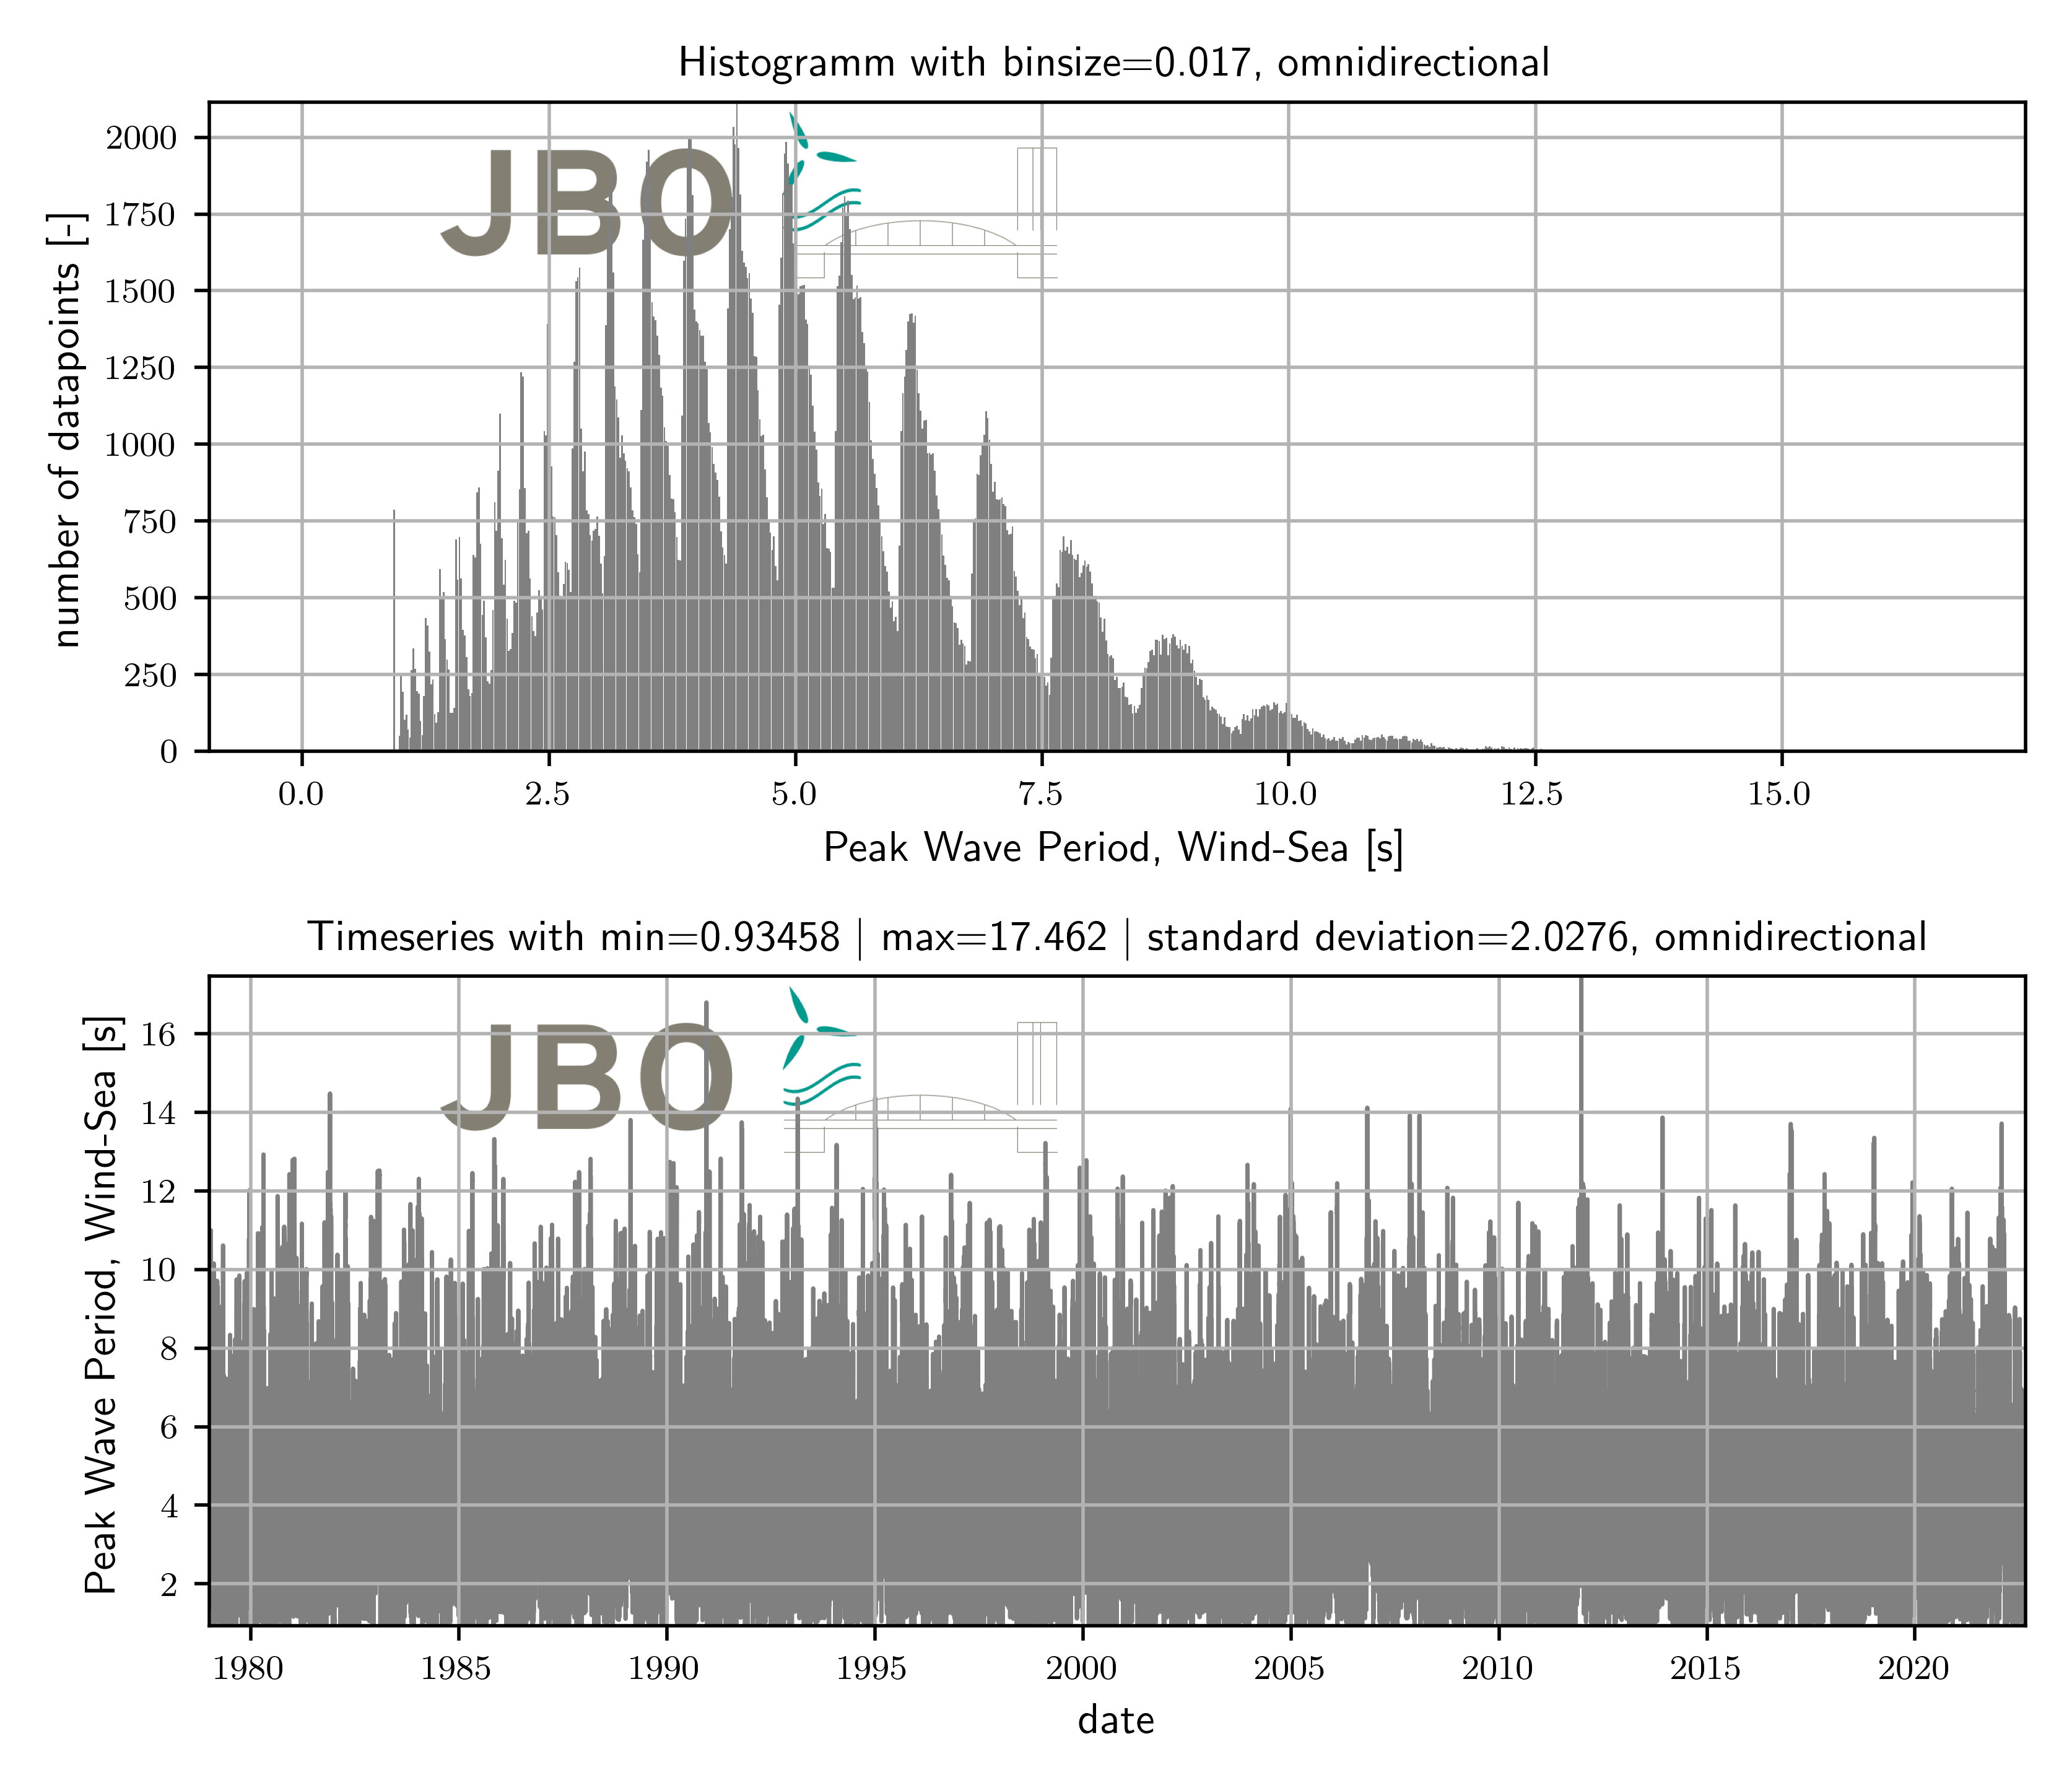
\includegraphics[width=1.0\textwidth]{C:/Users/aaron.lange/Desktop/Projekte/Hindcast_Tool/HindTool/example_output/SensorEval_T_p_wind_page_1.png} 
 \caption{ Timeseries and Histogram of Sensor: Peak Wave Period, Wind-Sea [s] } 
 \label{fig: SensorEval_T_p_wind_page_1 } 
\end{figure}
 \clearpage
\subsubsection{Sensor: Sign. Wave Height, Swell [m]} 
\begin{figure}[H] 
 \centering 
 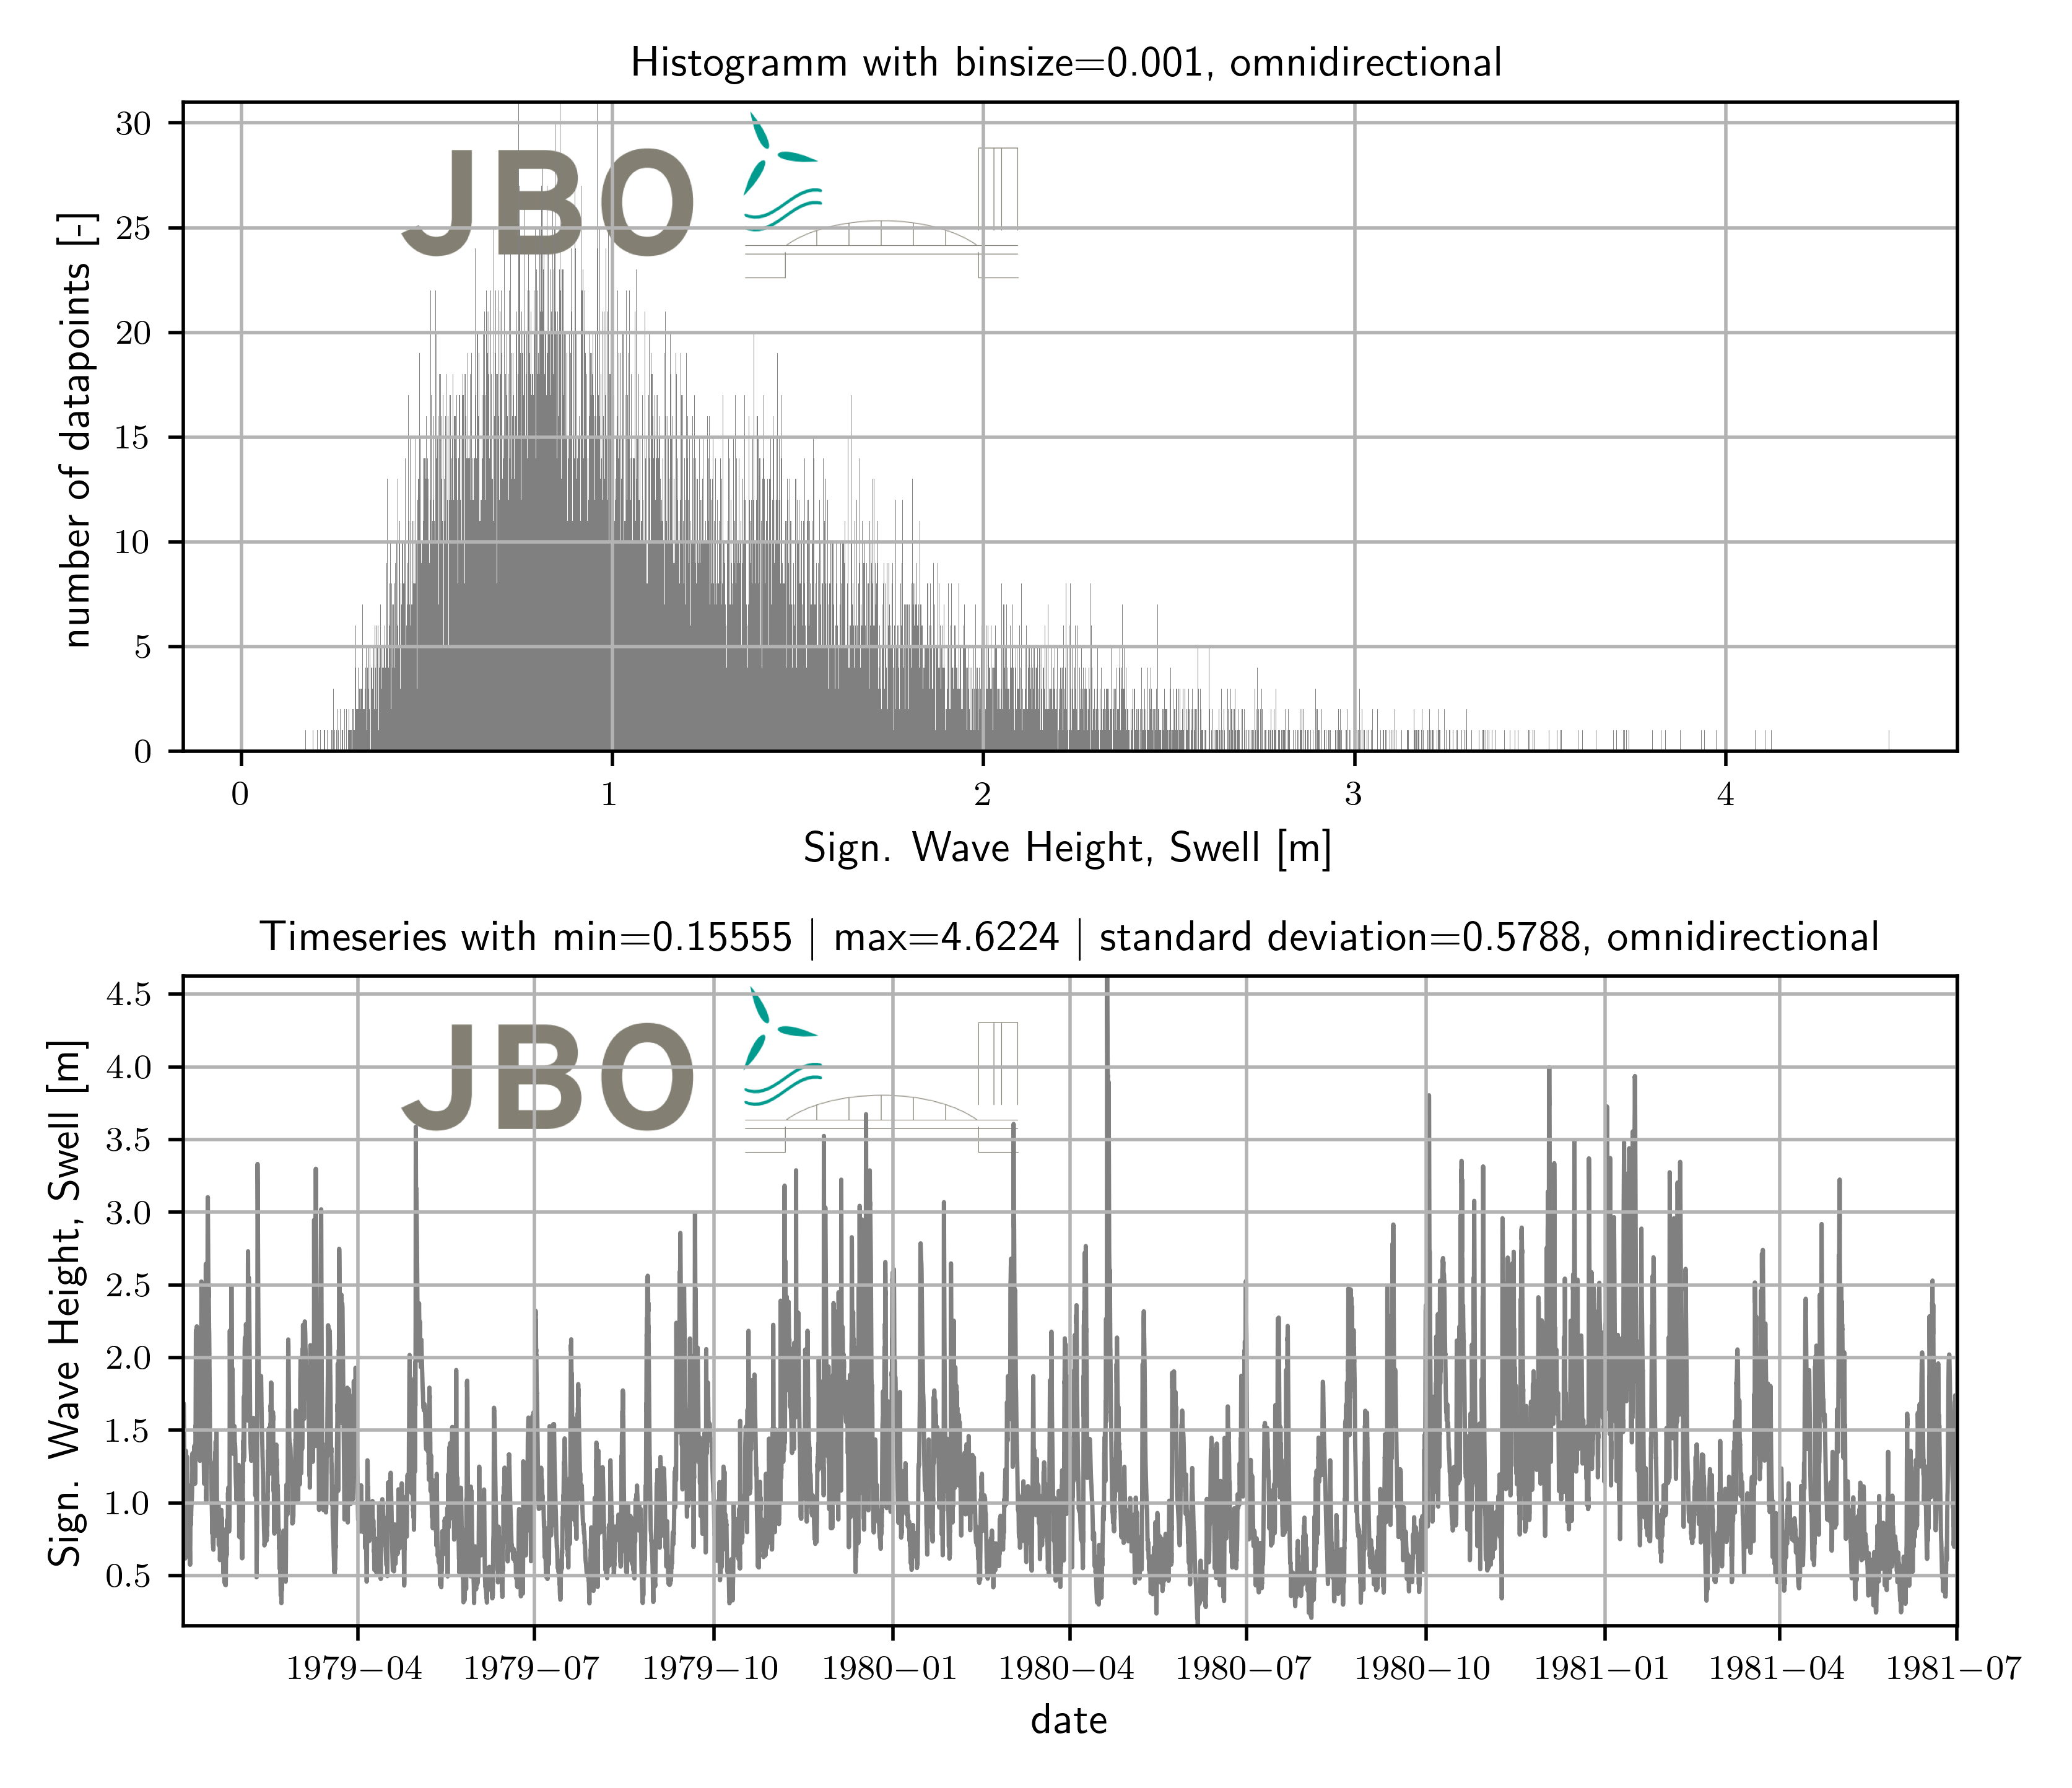
\includegraphics[width=1.0\textwidth]{C:/Users/aaron.lange/Desktop/Projekte/Hindcast_Tool/HindTool/example_output/SensorEval_H_s_swell_page_1.png} 
 \caption{ Timeseries and Histogram of Sensor: Sign. Wave Height, Swell [m] } 
 \label{fig: SensorEval_H_s_swell_page_1 } 
\end{figure}
 \clearpage
\subsubsection{Sensor: Peak Wave Period, Swell [s]} 
\begin{figure}[H] 
 \centering 
 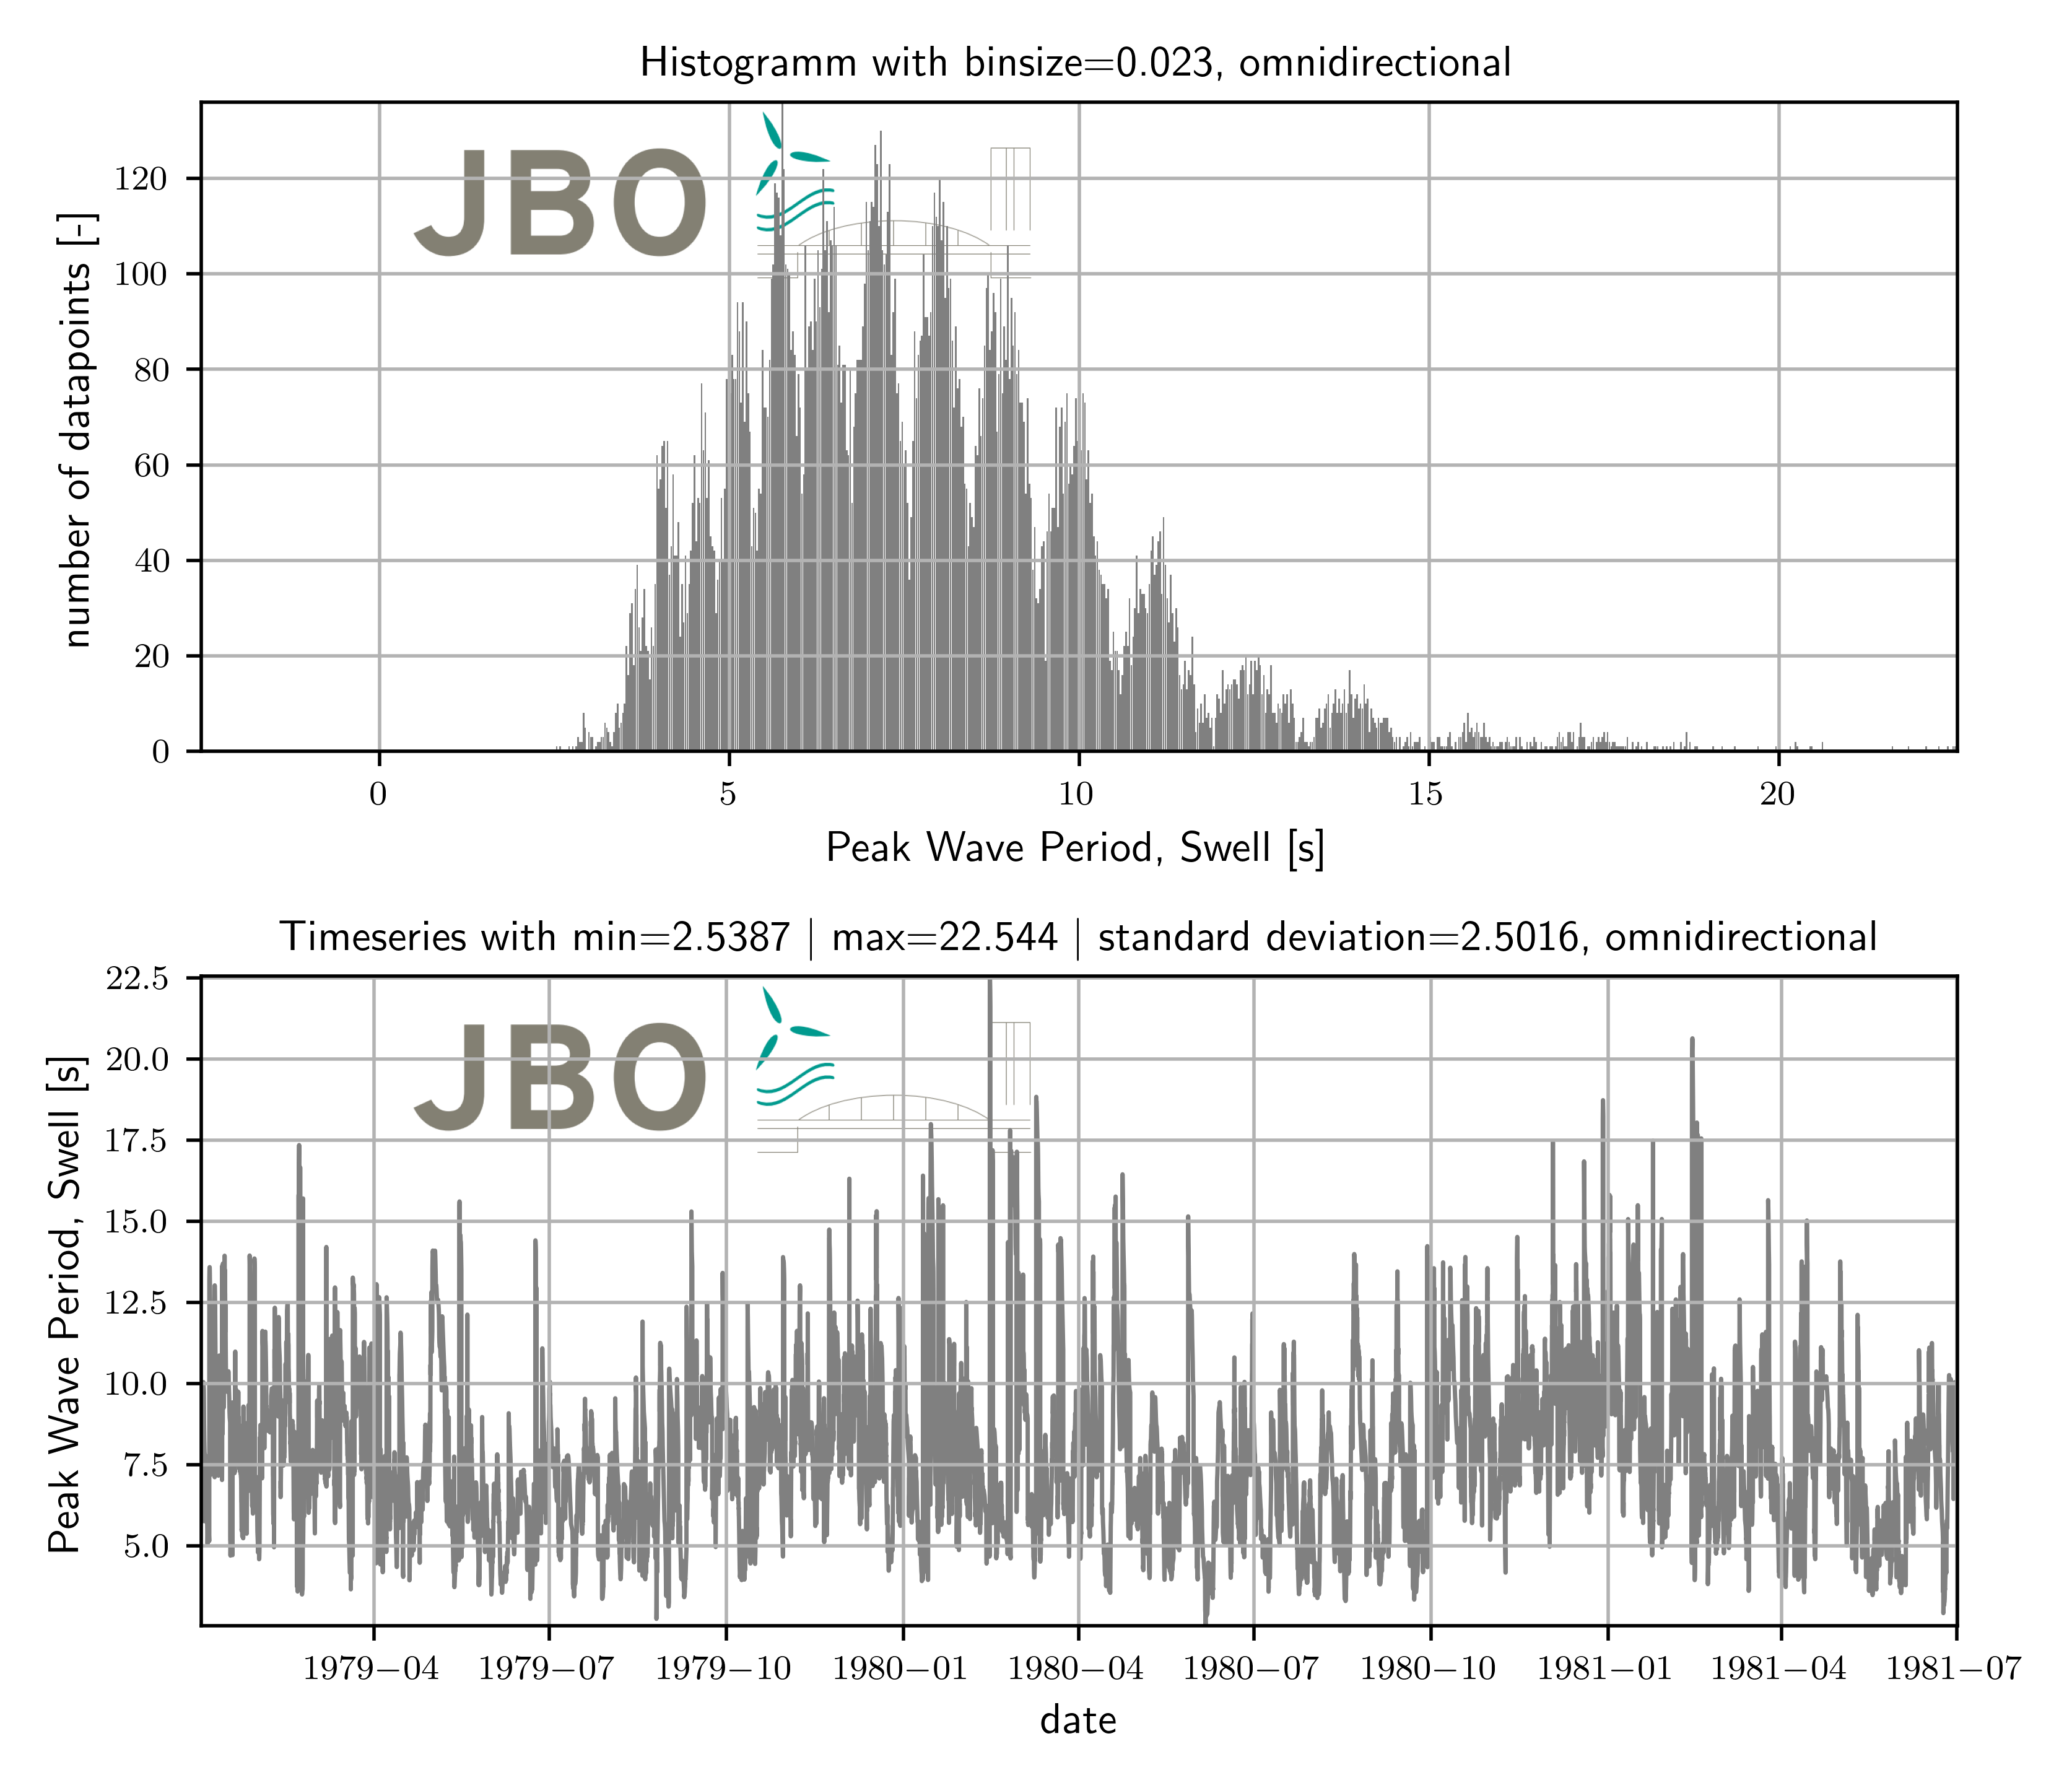
\includegraphics[width=1.0\textwidth]{C:/Users/aaron.lange/Desktop/Projekte/Hindcast_Tool/HindTool/example_output/SensorEval_T_p_swell_page_1.png} 
 \caption{ Timeseries and Histogram of Sensor: Peak Wave Period, Swell [s] } 
 \label{fig: SensorEval_T_p_swell_page_1 } 
\end{figure}
 \clearpage
\subsubsection{Sensor: Water Level [mMSL]} 
\begin{figure}[H] 
 \centering 
 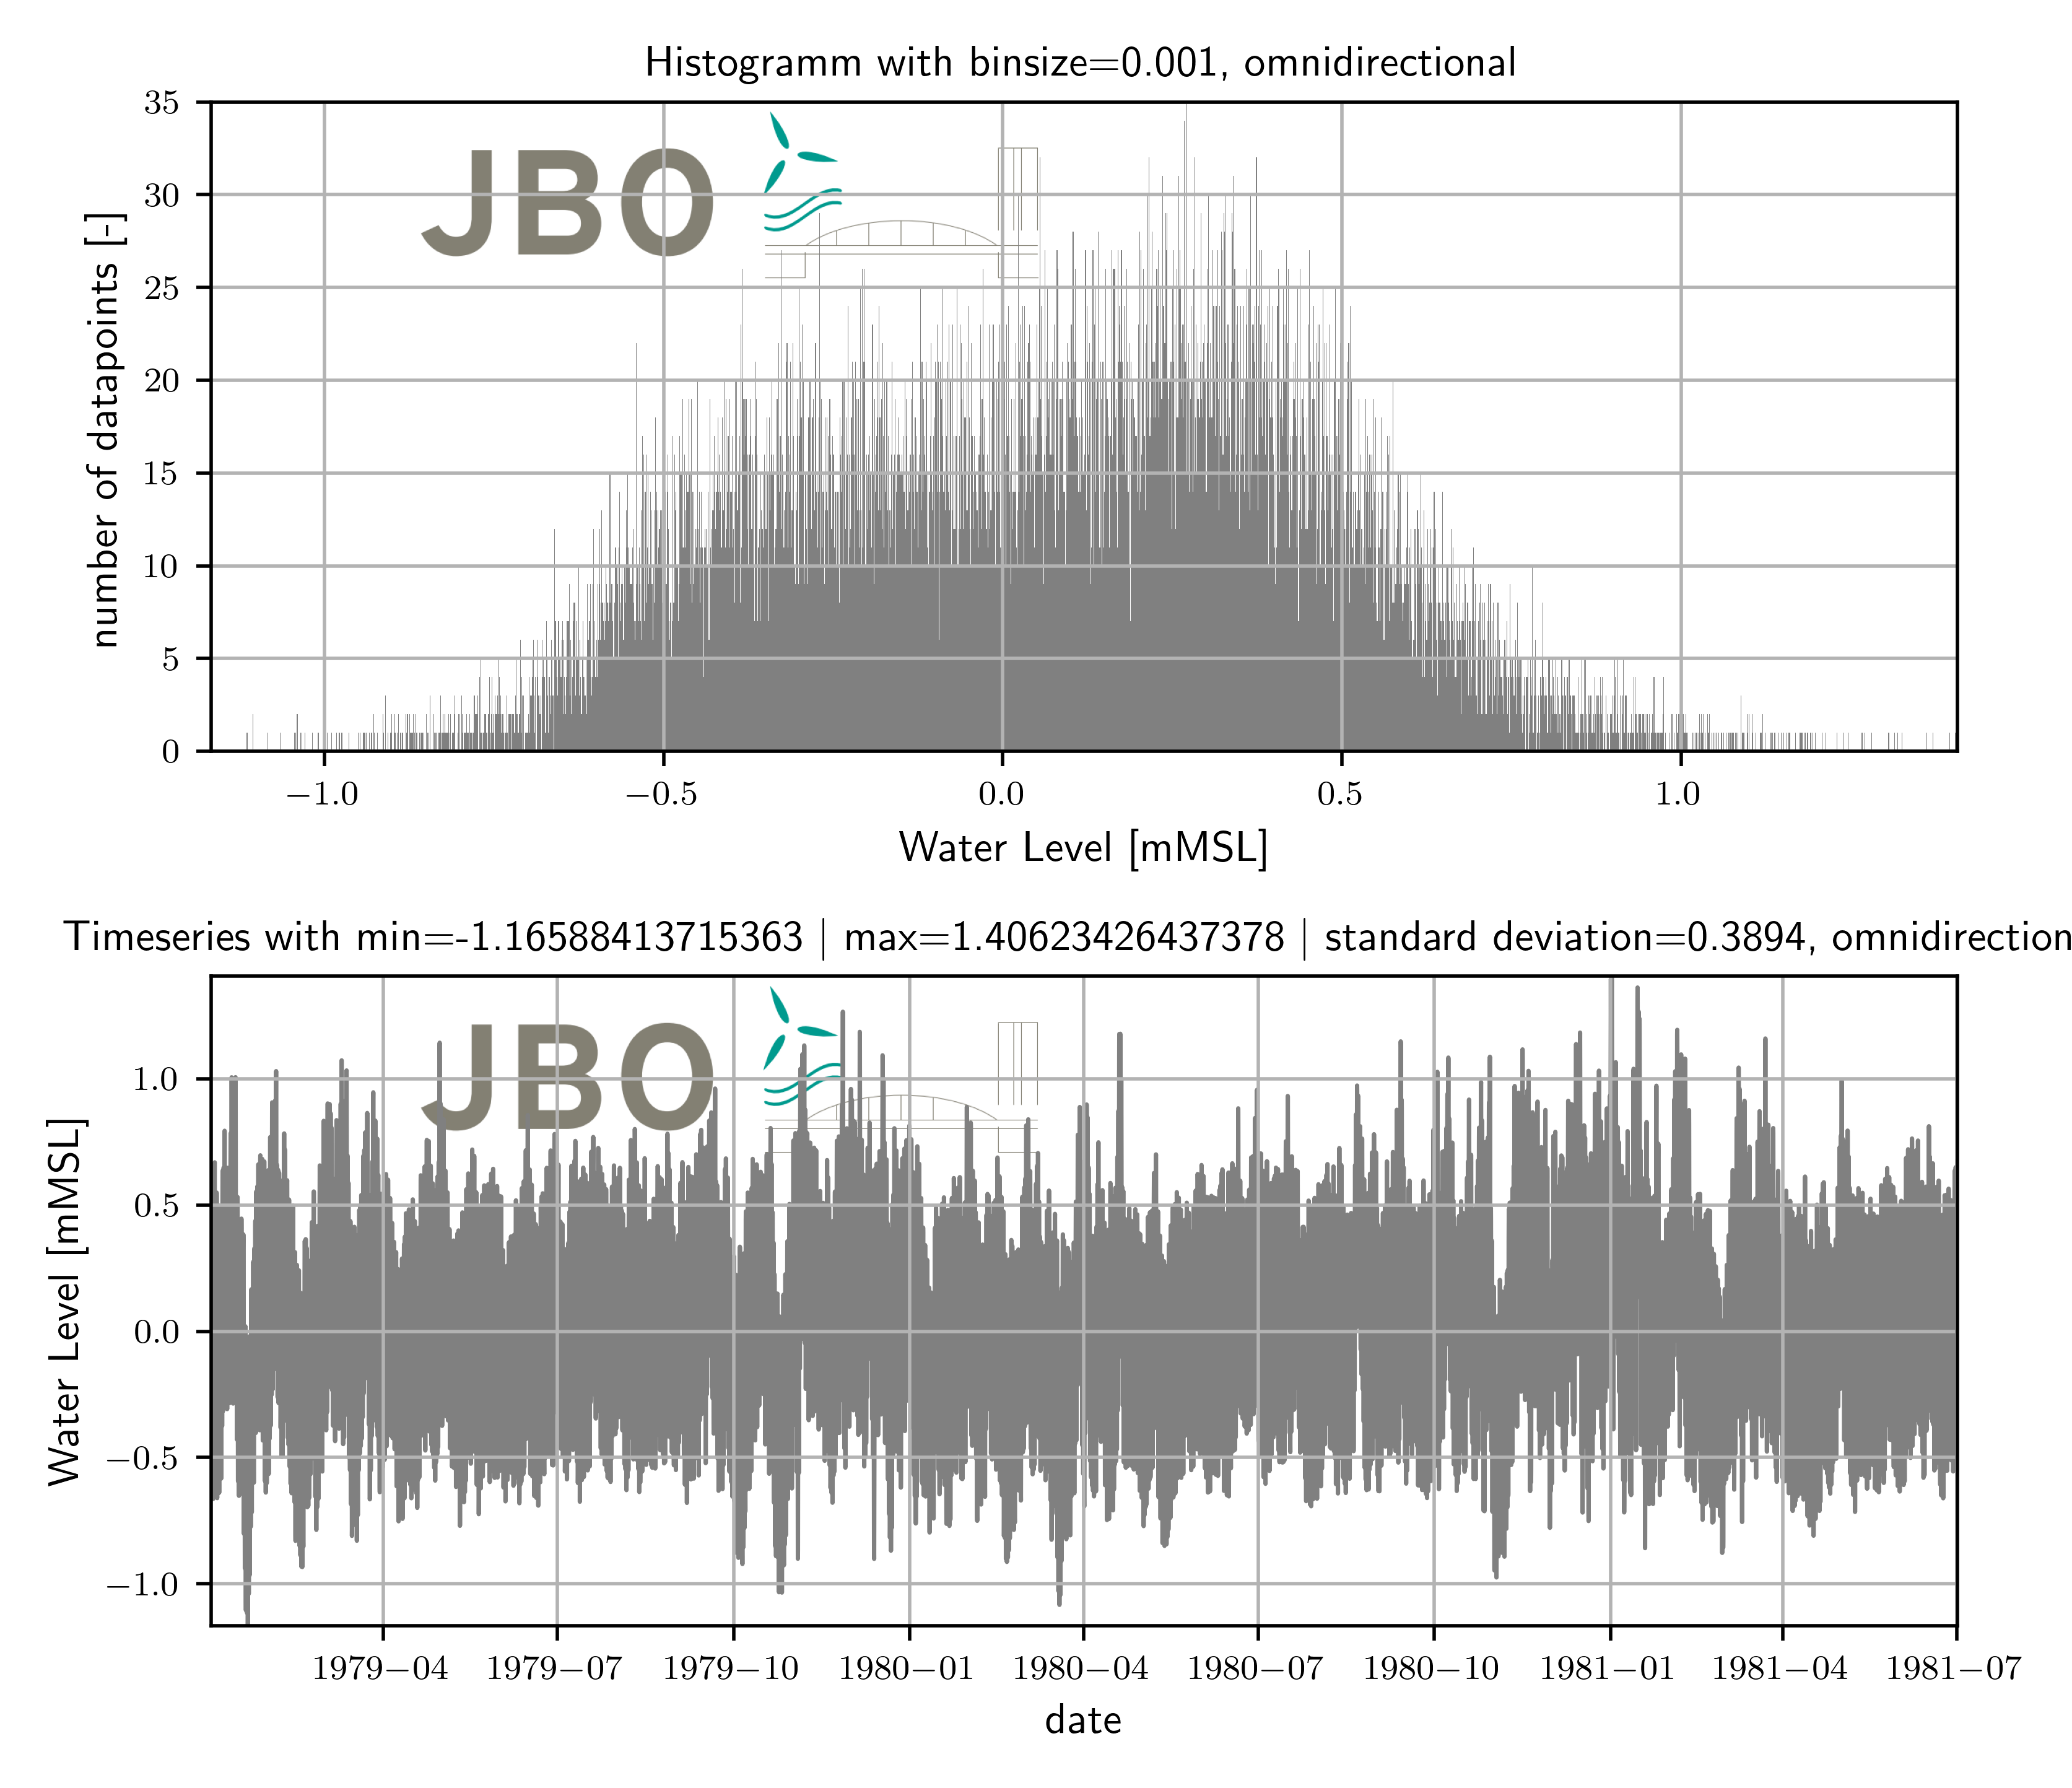
\includegraphics[width=1.0\textwidth]{C:/Users/aaron.lange/Desktop/Projekte/Hindcast_Tool/HindTool/example_output/SensorEval_WL_page_1.png} 
 \caption{ Timeseries and Histogram of Sensor: Water Level [mMSL] } 
 \label{fig: SensorEval_WL_page_1 } 
\end{figure}
 \clearpage
\subsubsection{Sensor: Water Level, Tide [mMSL]} 
\begin{figure}[H] 
 \centering 
 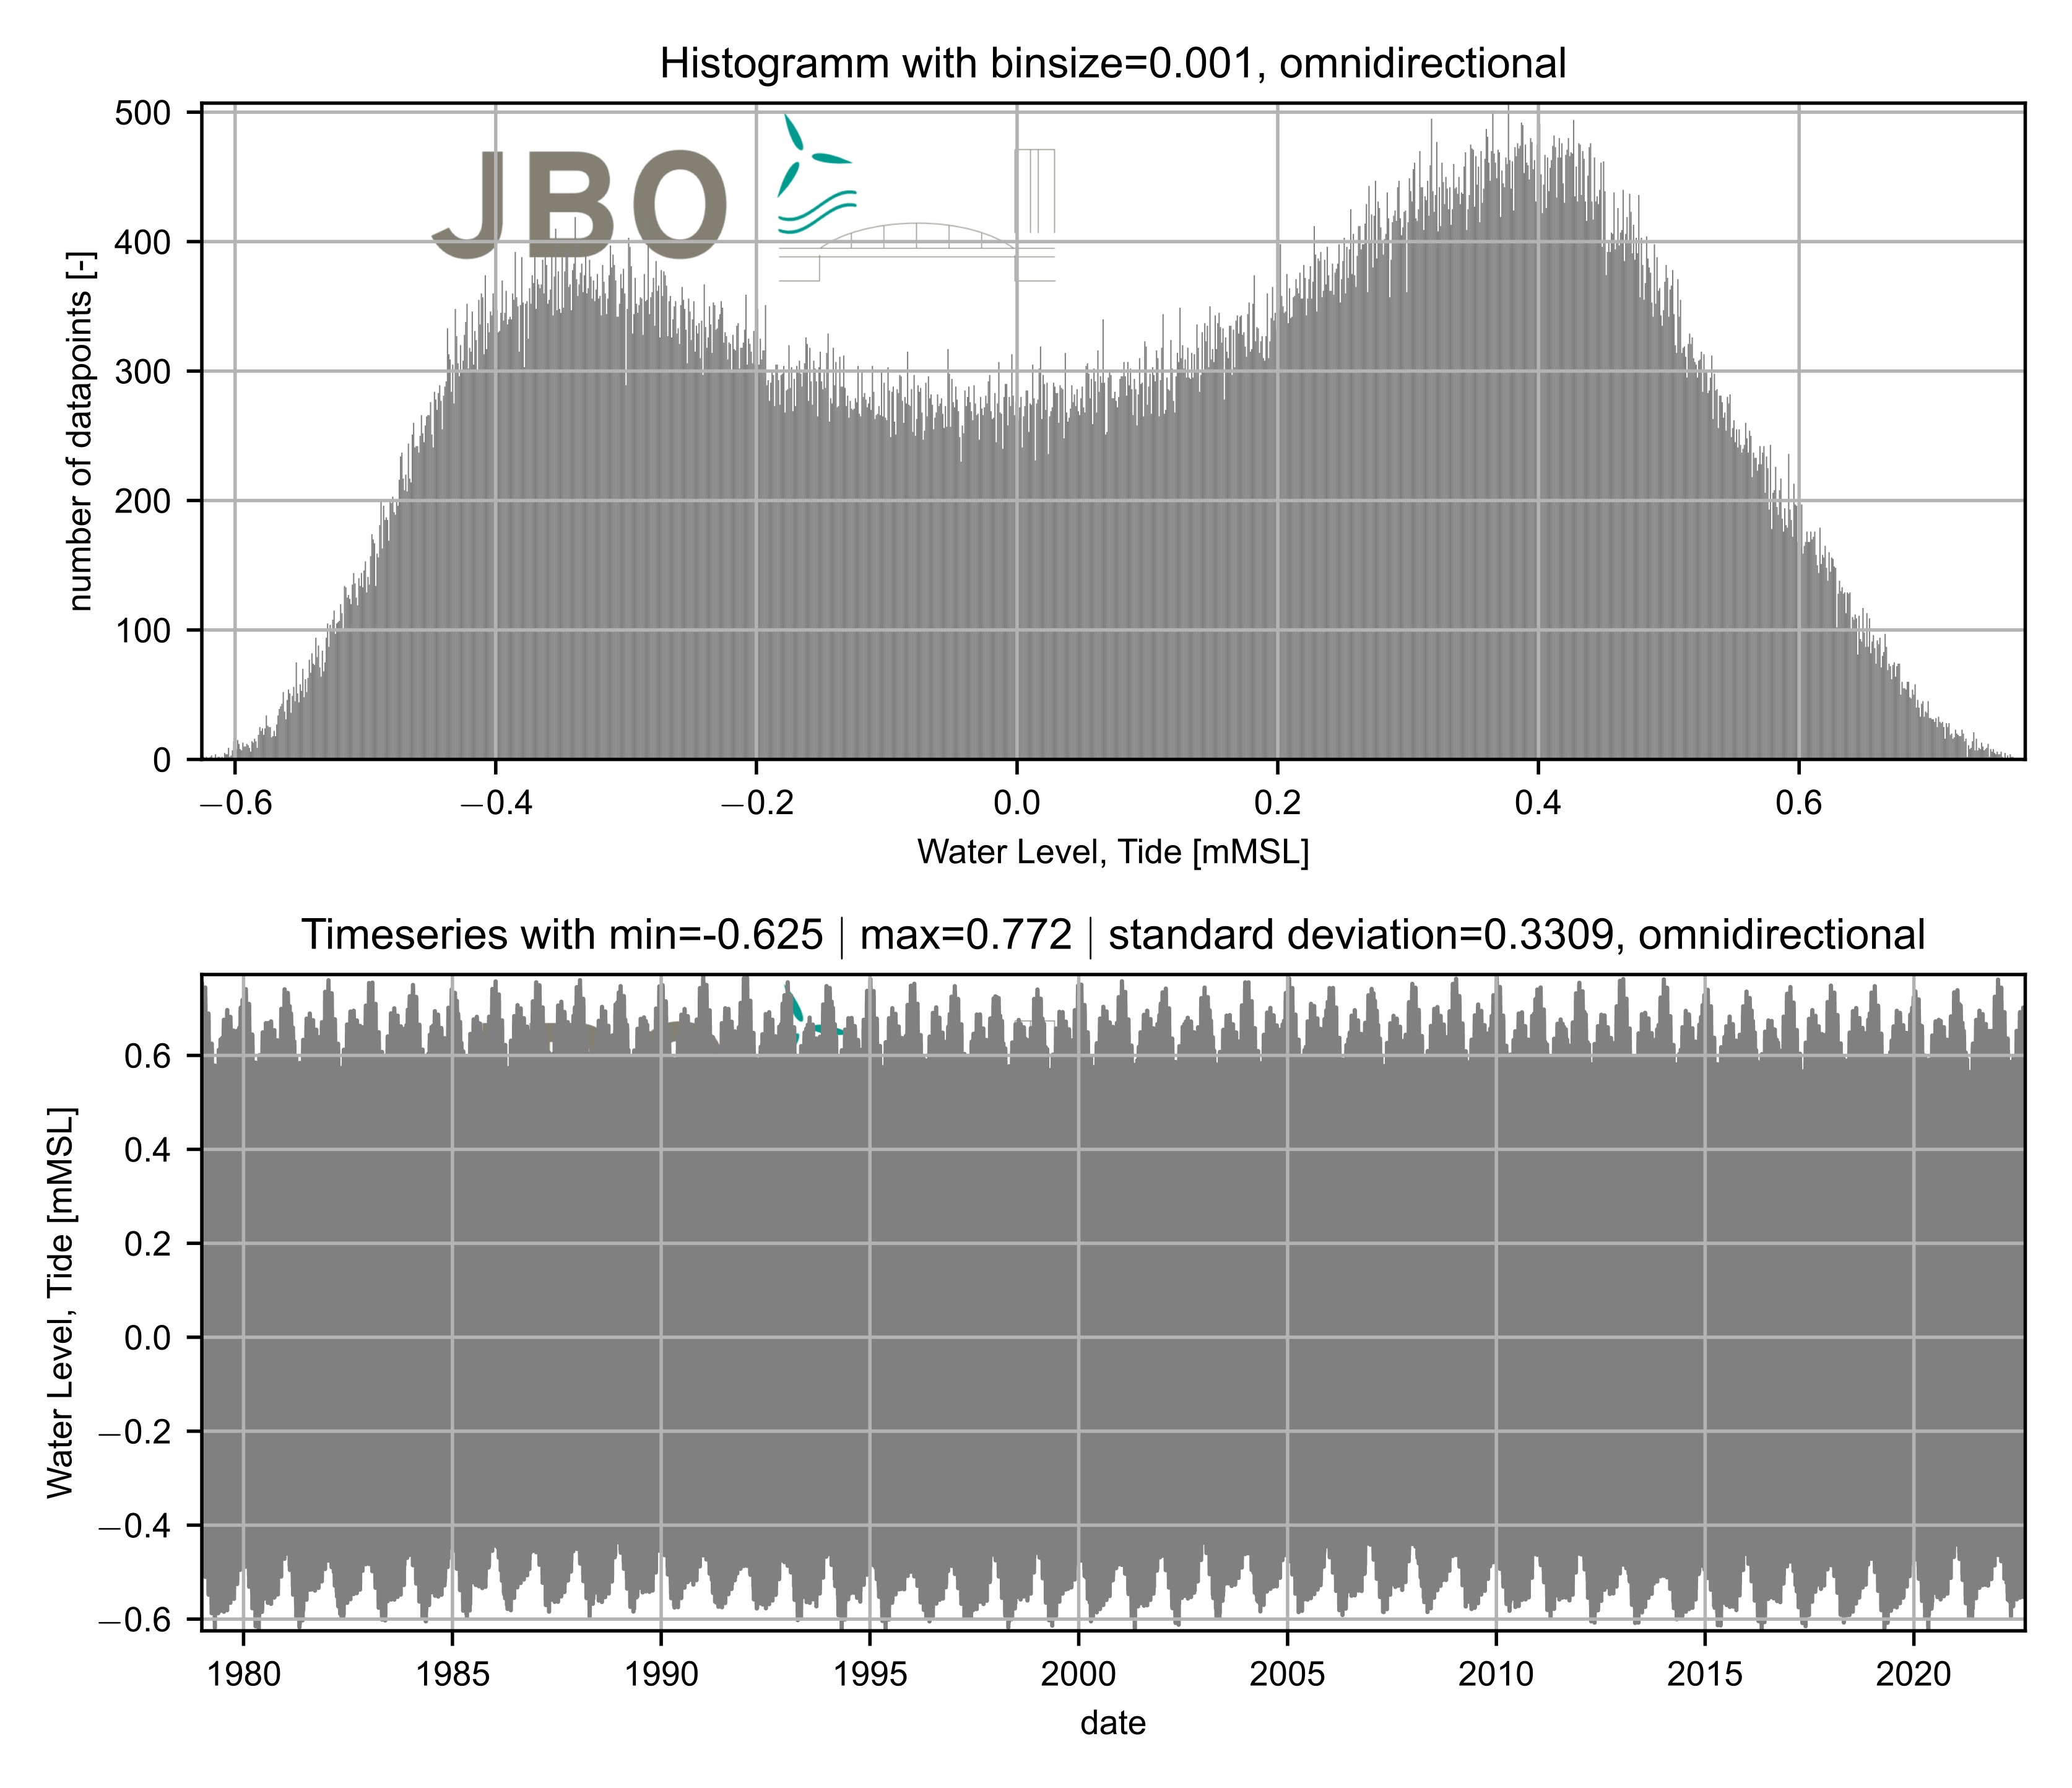
\includegraphics[width=1.0\textwidth]{C:/Users/aaron.lange/Desktop/Projekte/Hindcast_Tool/HindTool/example_output/SensorEval_WL_tide_page_1.png} 
 \caption{ Timeseries and Histogram of Sensor: Water Level, Tide [mMSL] } 
 \label{fig: SensorEval_WL_tide_page_1 } 
\end{figure}
 \clearpage
\subsubsection{Sensor: Current Speed Surface [m/s]} 
\begin{figure}[H] 
 \centering 
 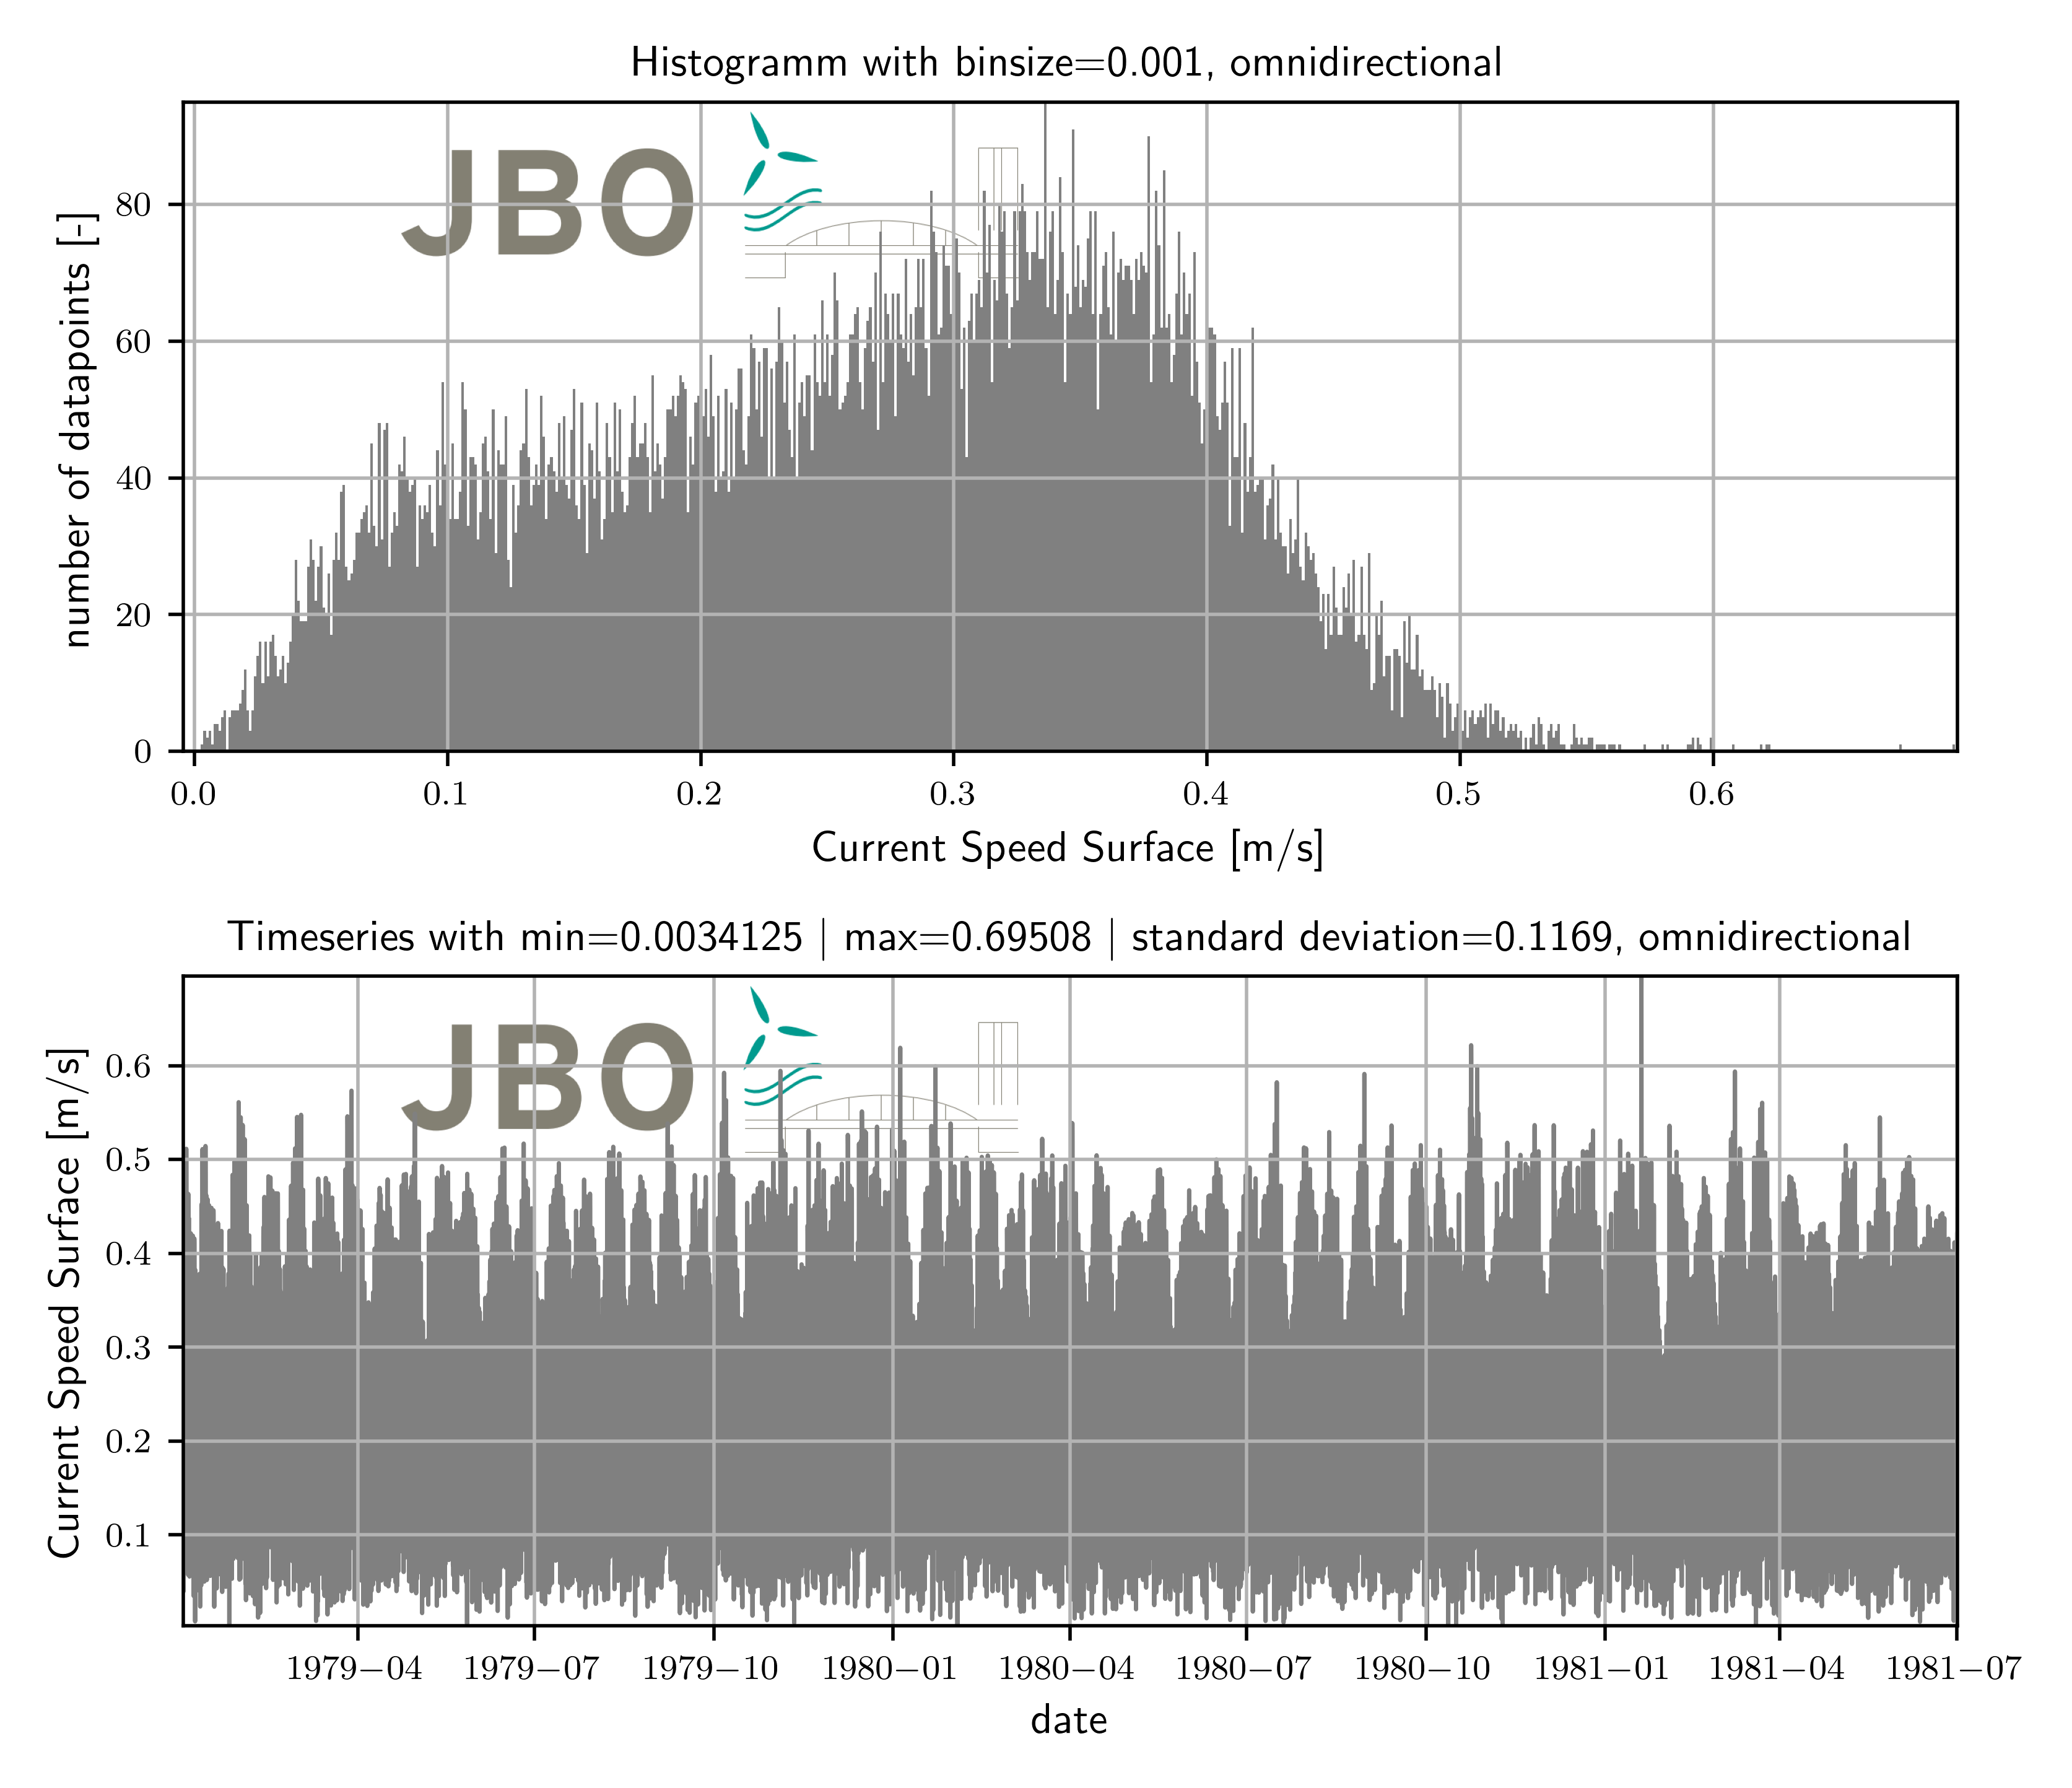
\includegraphics[width=1.0\textwidth]{C:/Users/aaron.lange/Desktop/Projekte/Hindcast_Tool/HindTool/example_output/SensorEval_v_curr_page_1.png} 
 \caption{ Timeseries and Histogram of Sensor: Current Speed Surface [m/s] } 
 \label{fig: SensorEval_v_curr_page_1 } 
\end{figure}
 \clearpage

\subsection{Sensor directional analysis}
Relevant directional sensor evaluations are shown below. 

\subsubsection{Wind direction and wind speed occurrence}

\begin{figure}[H] 
 \centering 
 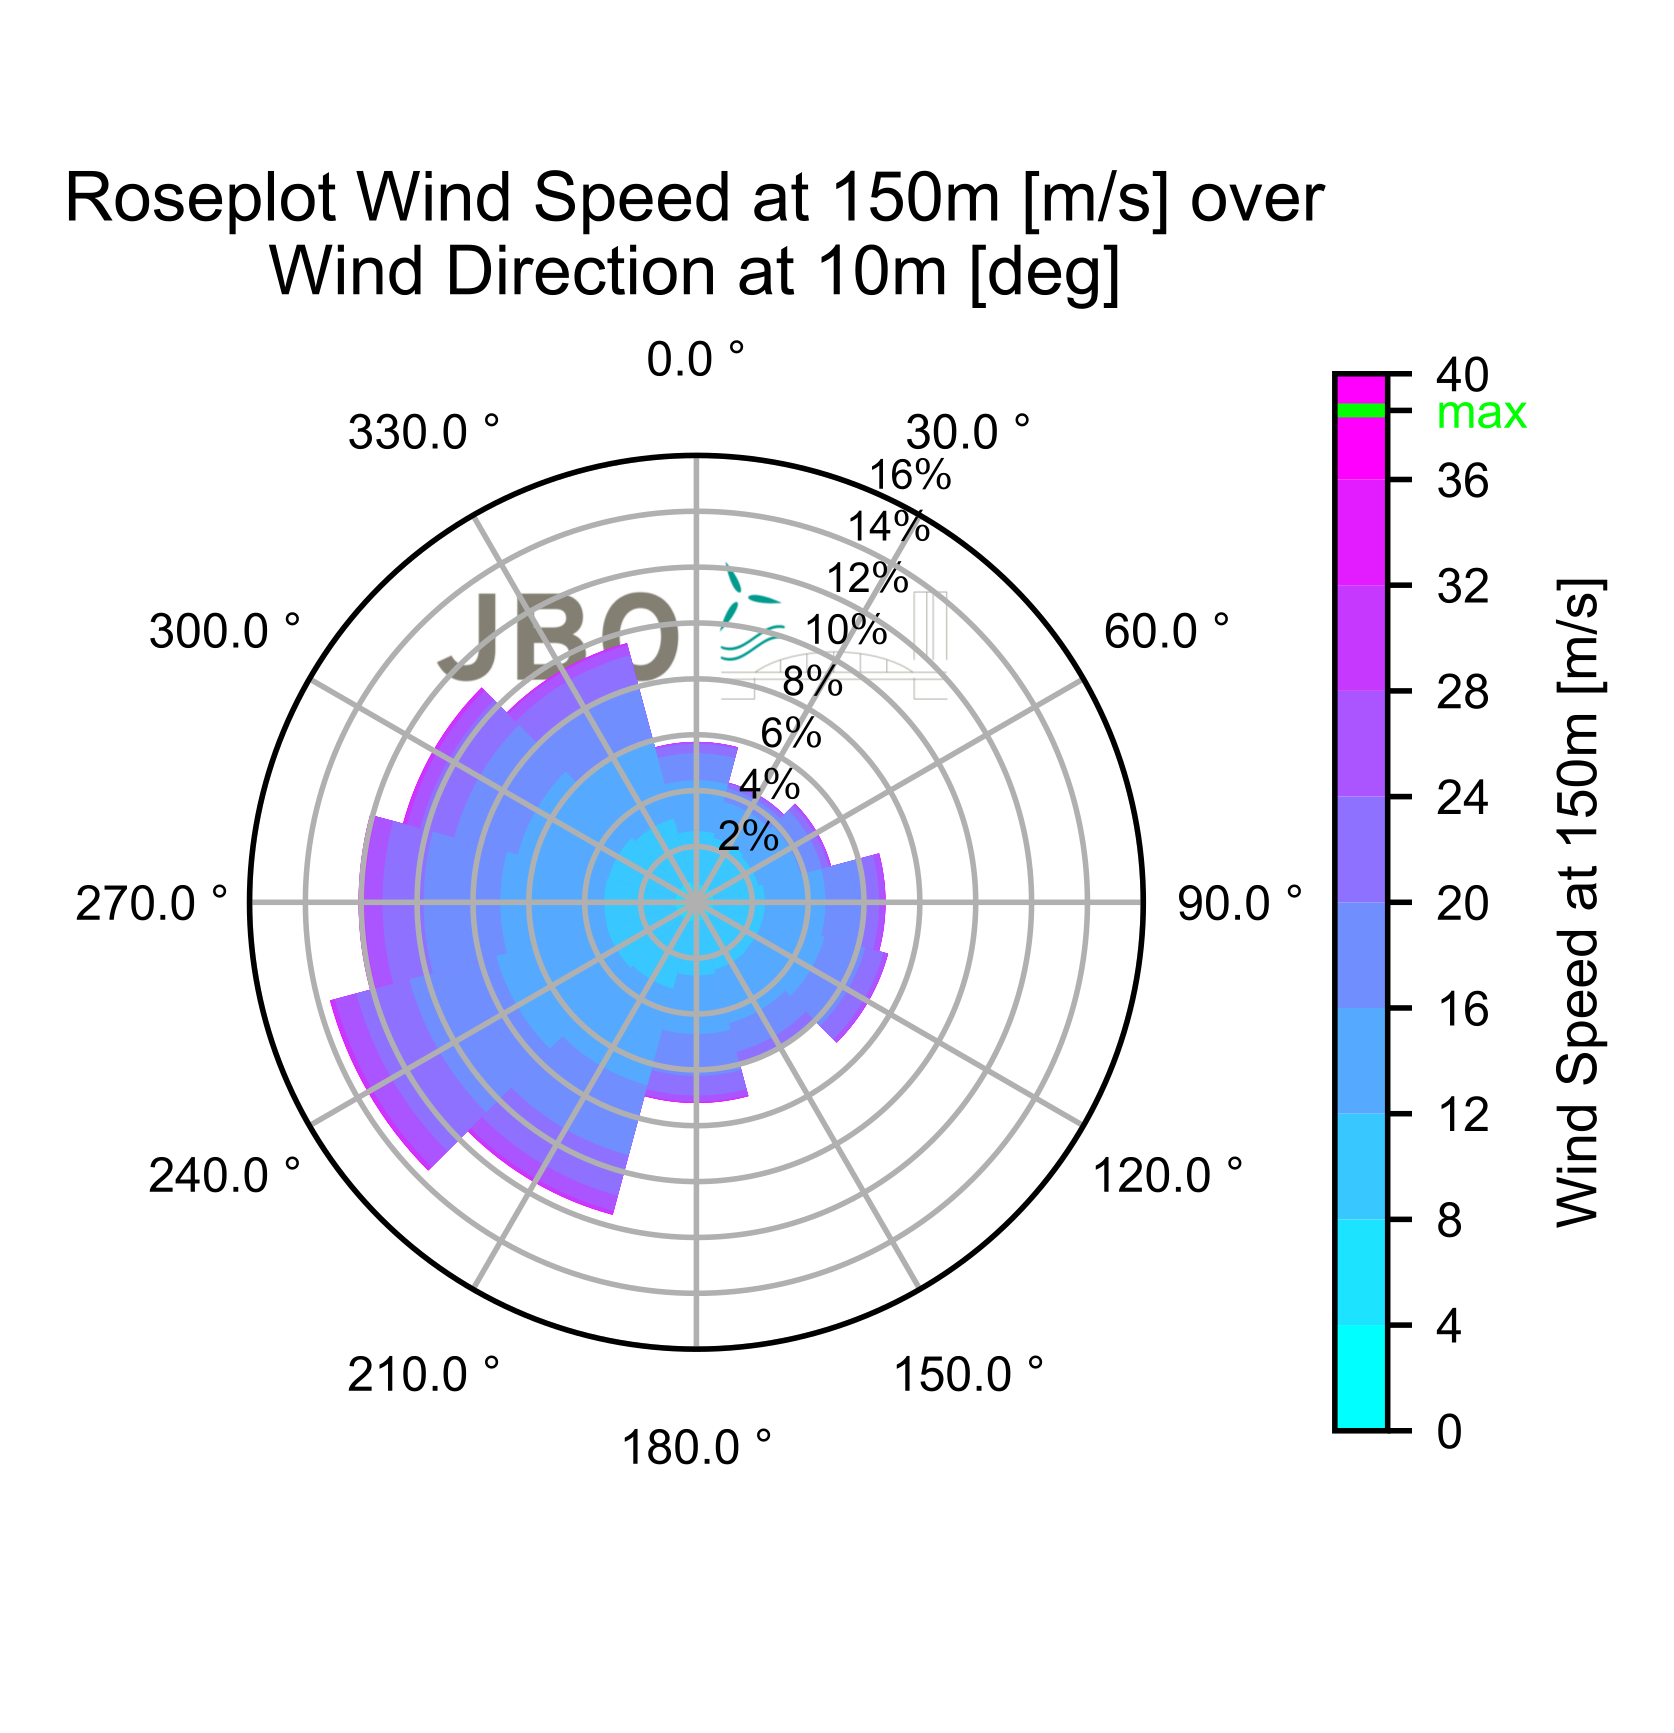
\includegraphics[width=1.0\textwidth]{C:/Users/aaron.lange/Desktop/Projekte/Hindcast_Tool/HindTool/example_output/Roseplots_wind_page_1.png} 
 \caption{ Roseplots-wind-page-1 } 
 \label{fig: Roseplots_wind_page_1 } 
\end{figure}

\subsubsection{Wave direction - Wind Sea}

\begin{figure}[H] 
 \centering 
 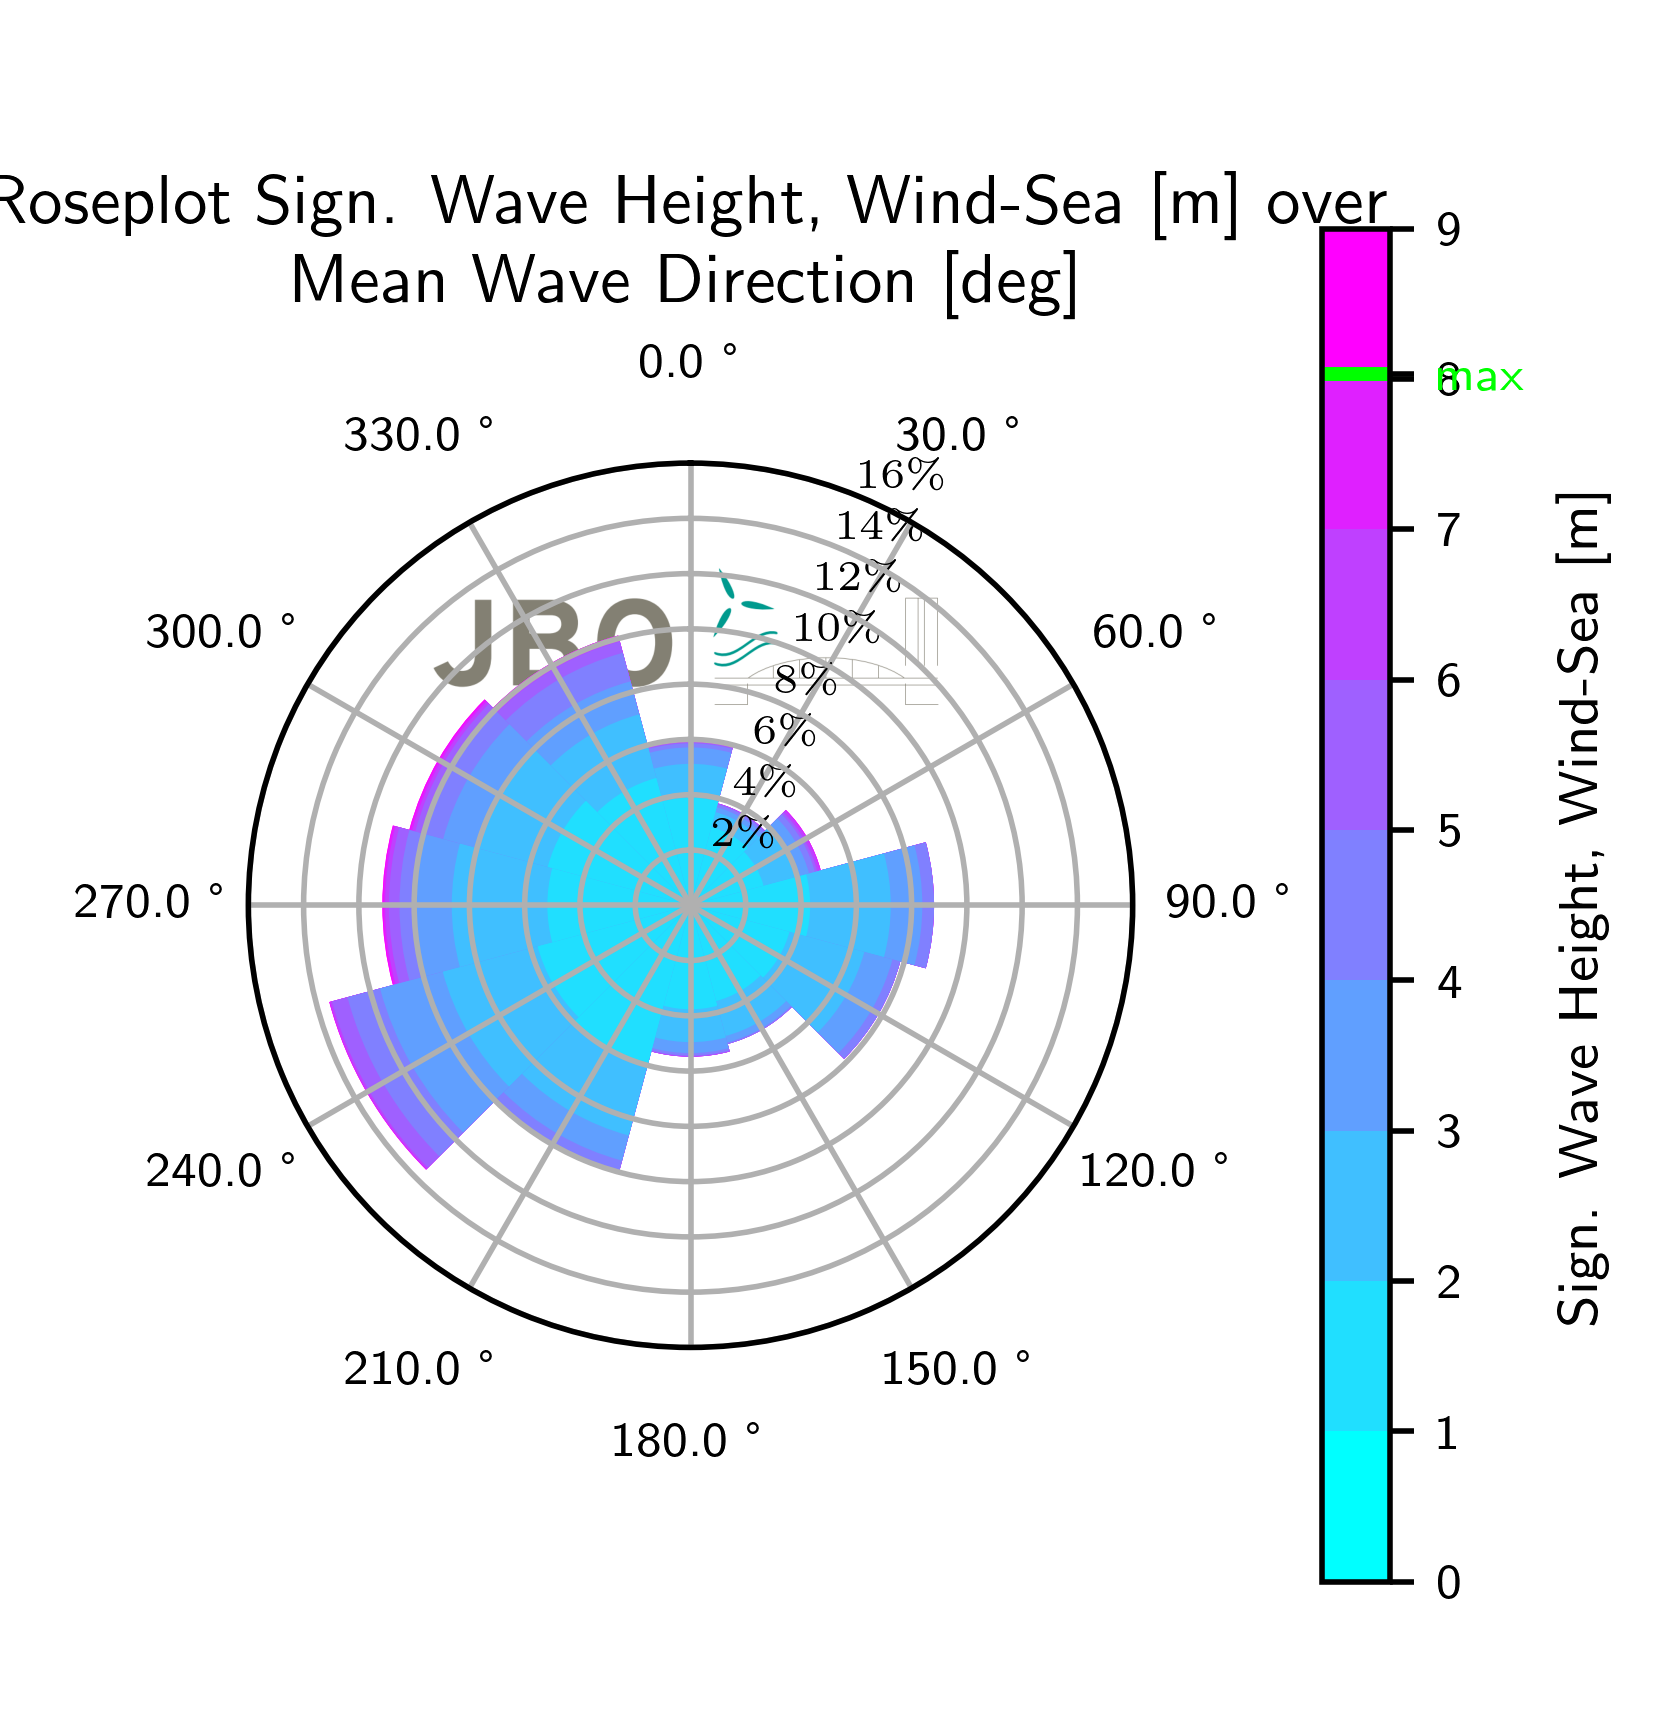
\includegraphics[width=1.0\textwidth]{C:/Users/aaron.lange/Desktop/Projekte/Hindcast_Tool/HindTool/example_output/Roseplots_wind_sea_page_1.png} 
 \caption{ Roseplots-wind-sea-page-1 } 
 \label{fig: Roseplots_wind_sea_page_1 } 
\end{figure}

\subsubsection{Wavedirection - Swell Sea}

\begin{figure}[H] 
 \centering 
 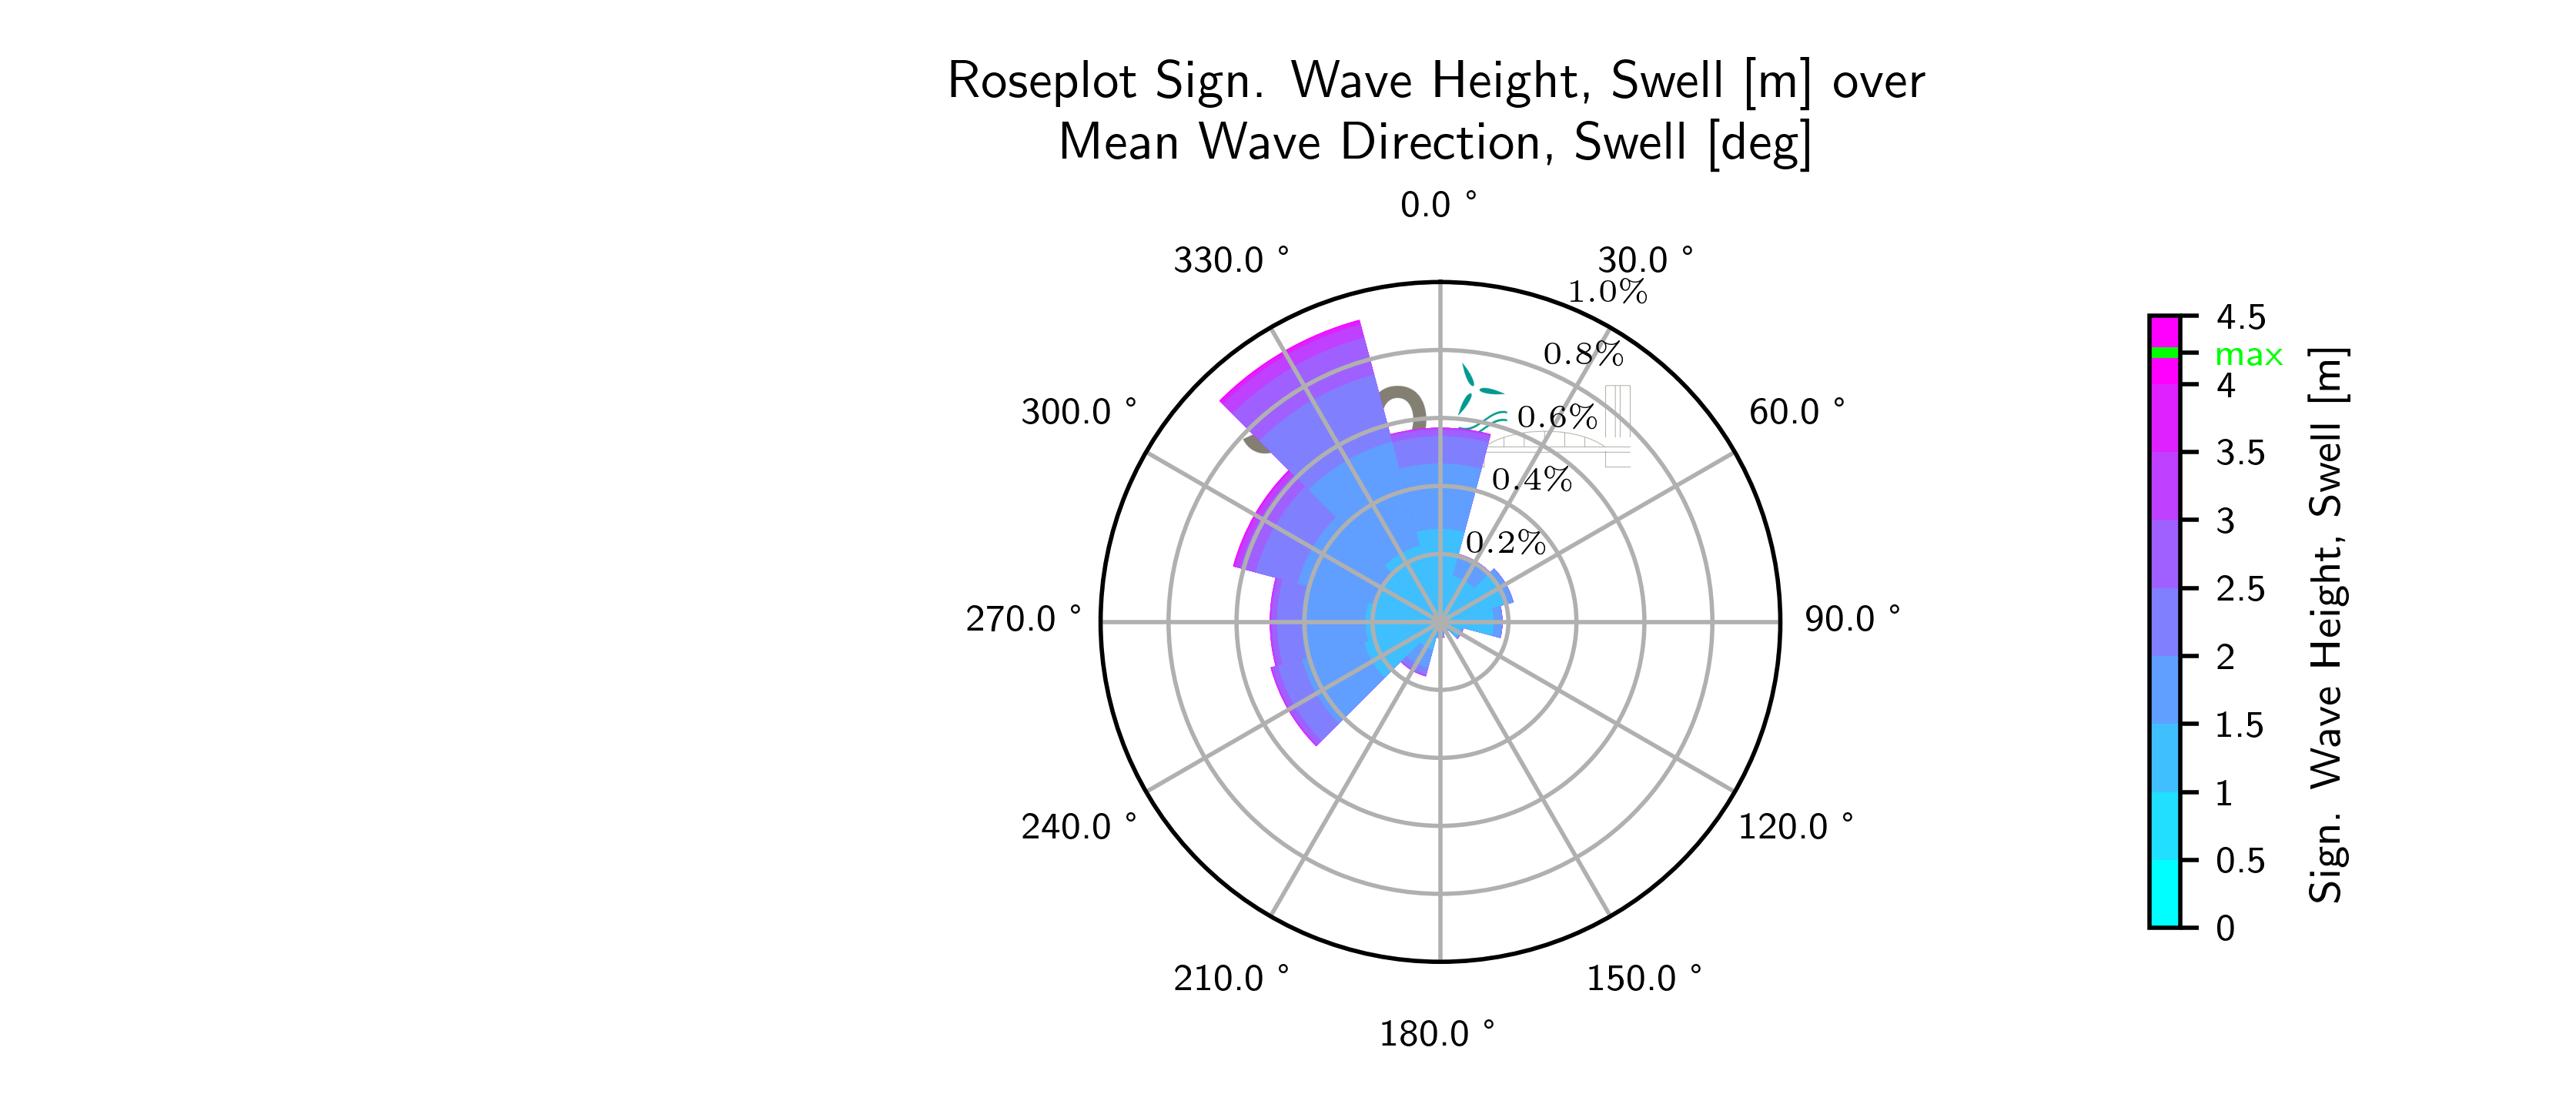
\includegraphics[width=1.0\textwidth]{C:/Users/aaron.lange/Desktop/Projekte/Hindcast_Tool/HindTool/example_output/Roseplots_swell_sea_page_1.png} 
 \caption{ Roseplots-swell-sea-page-1 } 
 \label{fig: Roseplots_swell_sea_page_1 } 
\end{figure}

\subsubsection{Wind - Wave Misalignment}

The occurrence probability of the wind direction and wave direction is considered for normal sea state condition. The misalignment of wind and wave direction, based on the wind direction, is illustrated below. 

\begin{figure}[H] 
 \centering 
 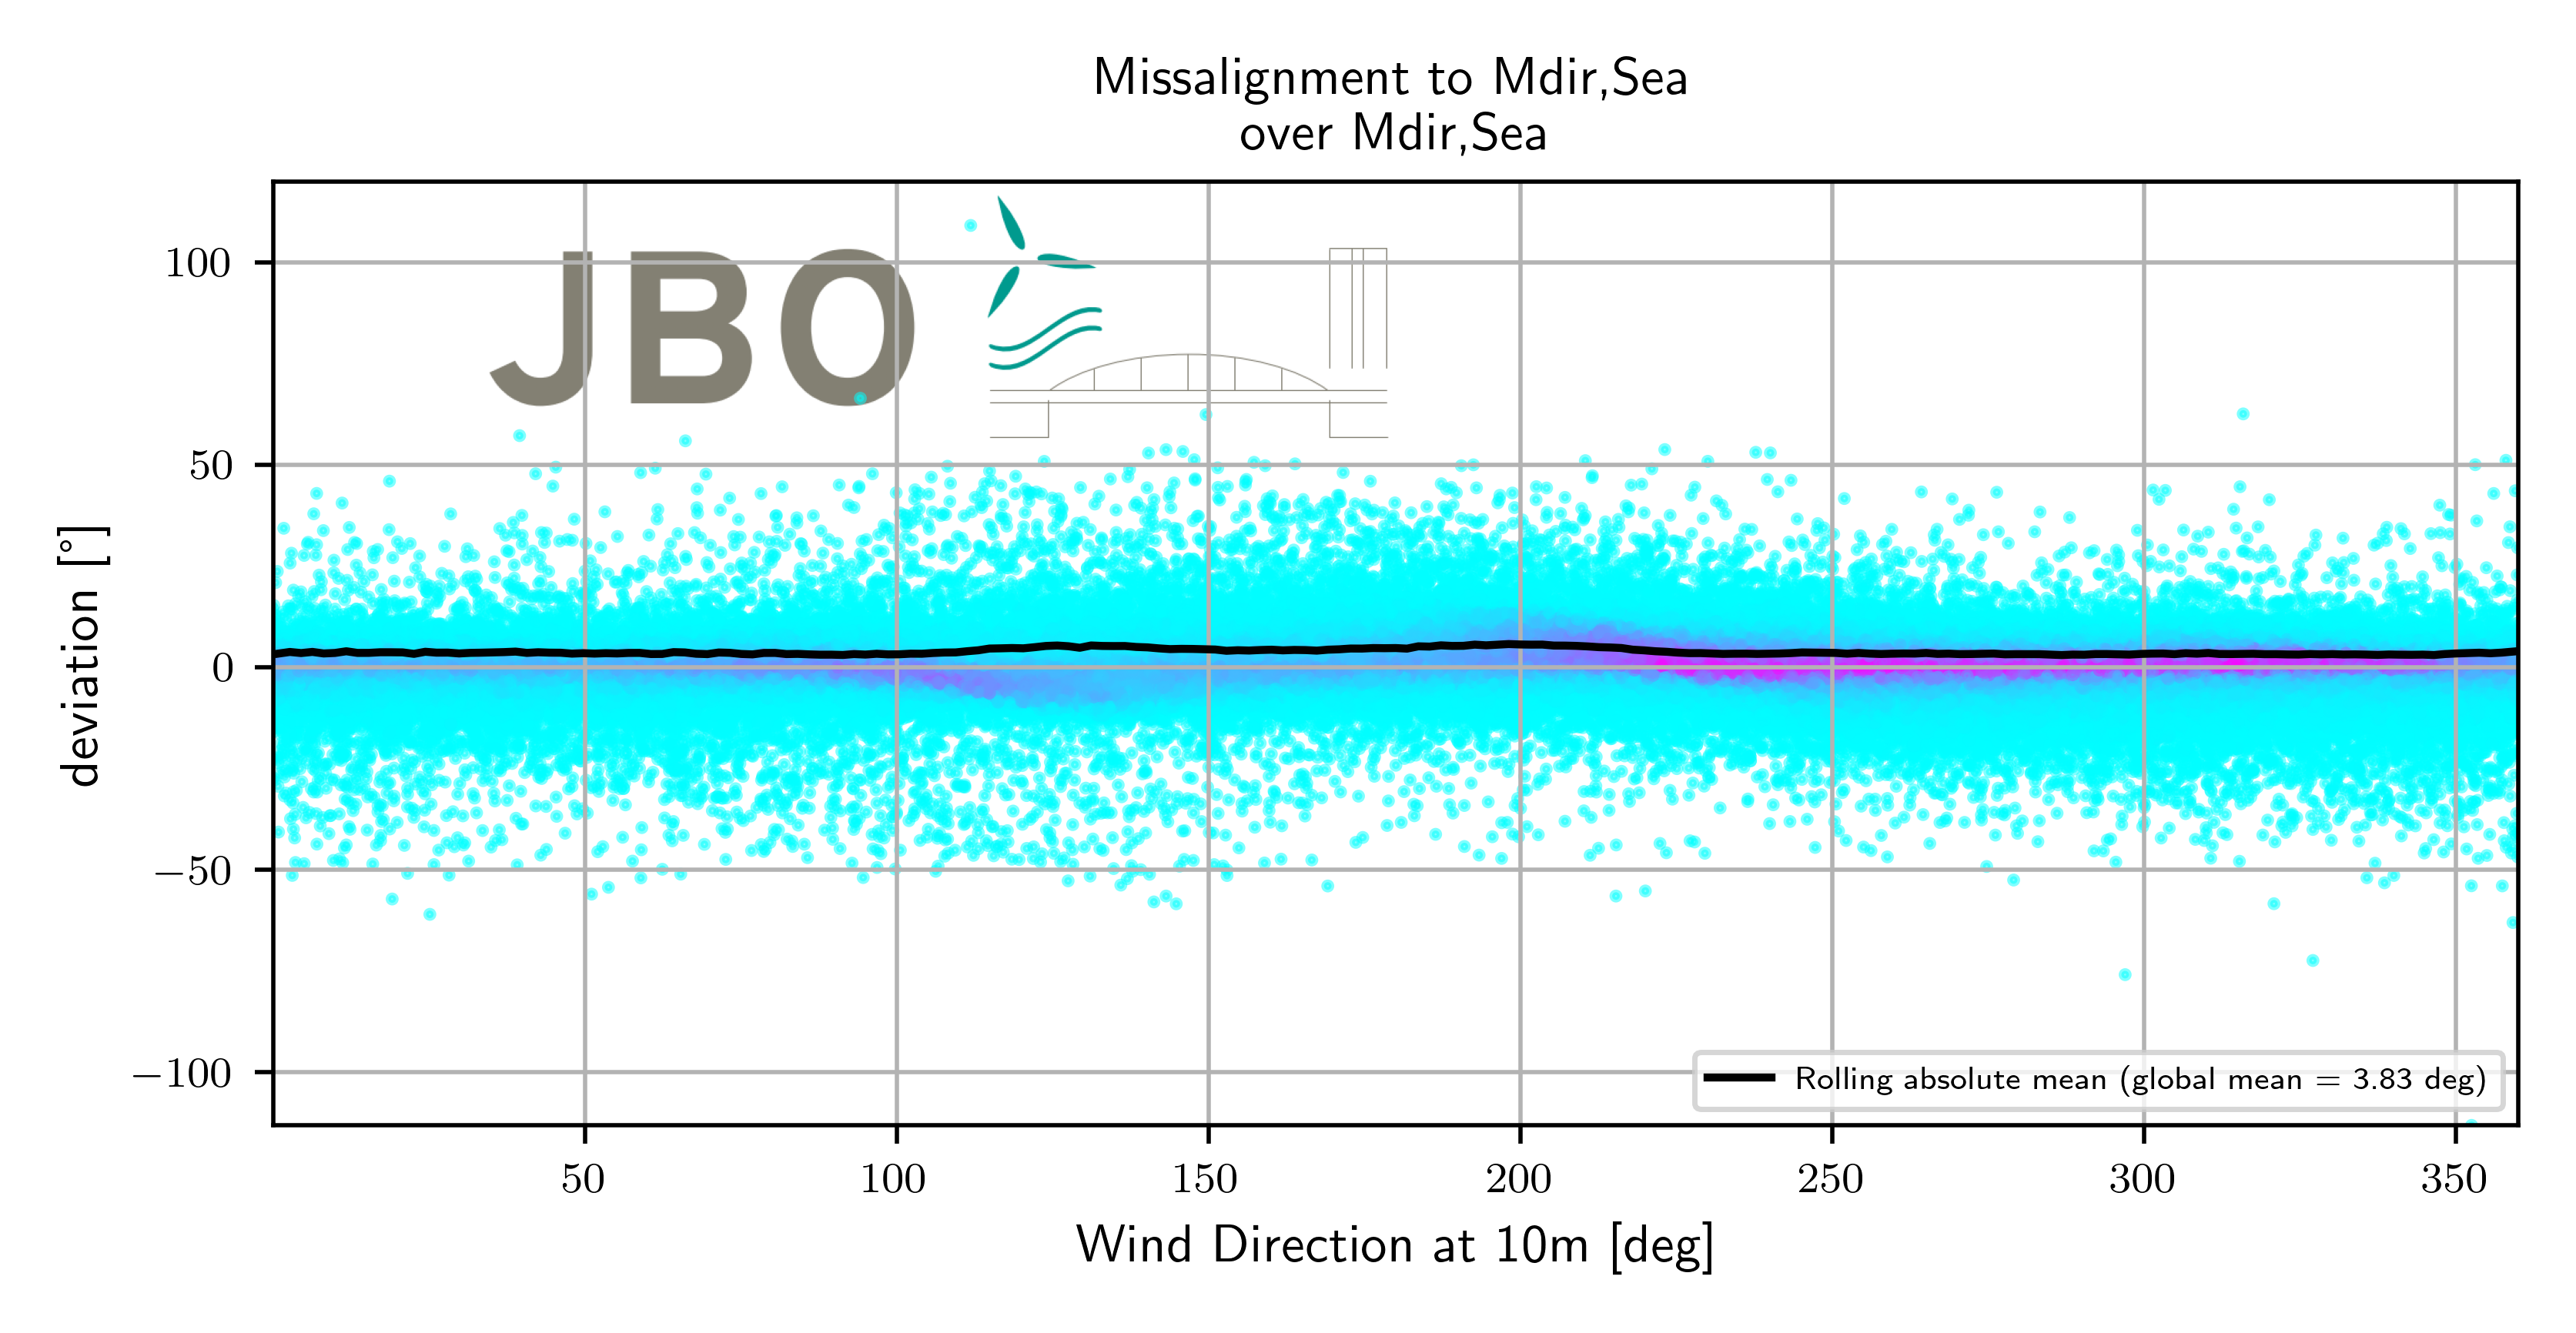
\includegraphics[width=1.0\textwidth]{C:/Users/aaron.lange/Desktop/Projekte/Hindcast_Tool/HindTool/example_output/angle_deviation_scatter_page_1.png} 
 \caption{ angle-deviation-scatter-page-1 } 
 \label{fig: angle_deviation_scatter_page_1 } 
\end{figure}

For the assignment of probabilities to the load situations in the design load case table, the data set is evaluated for each wind speed bin (delta = 1 m/s), wind direction and wave direction, both with a sector width of 30° (see Appendix). 


\clearpage
\subsubsection{Current direction and current speed occurrence}

\begin{figure}[H] 
 \centering 
 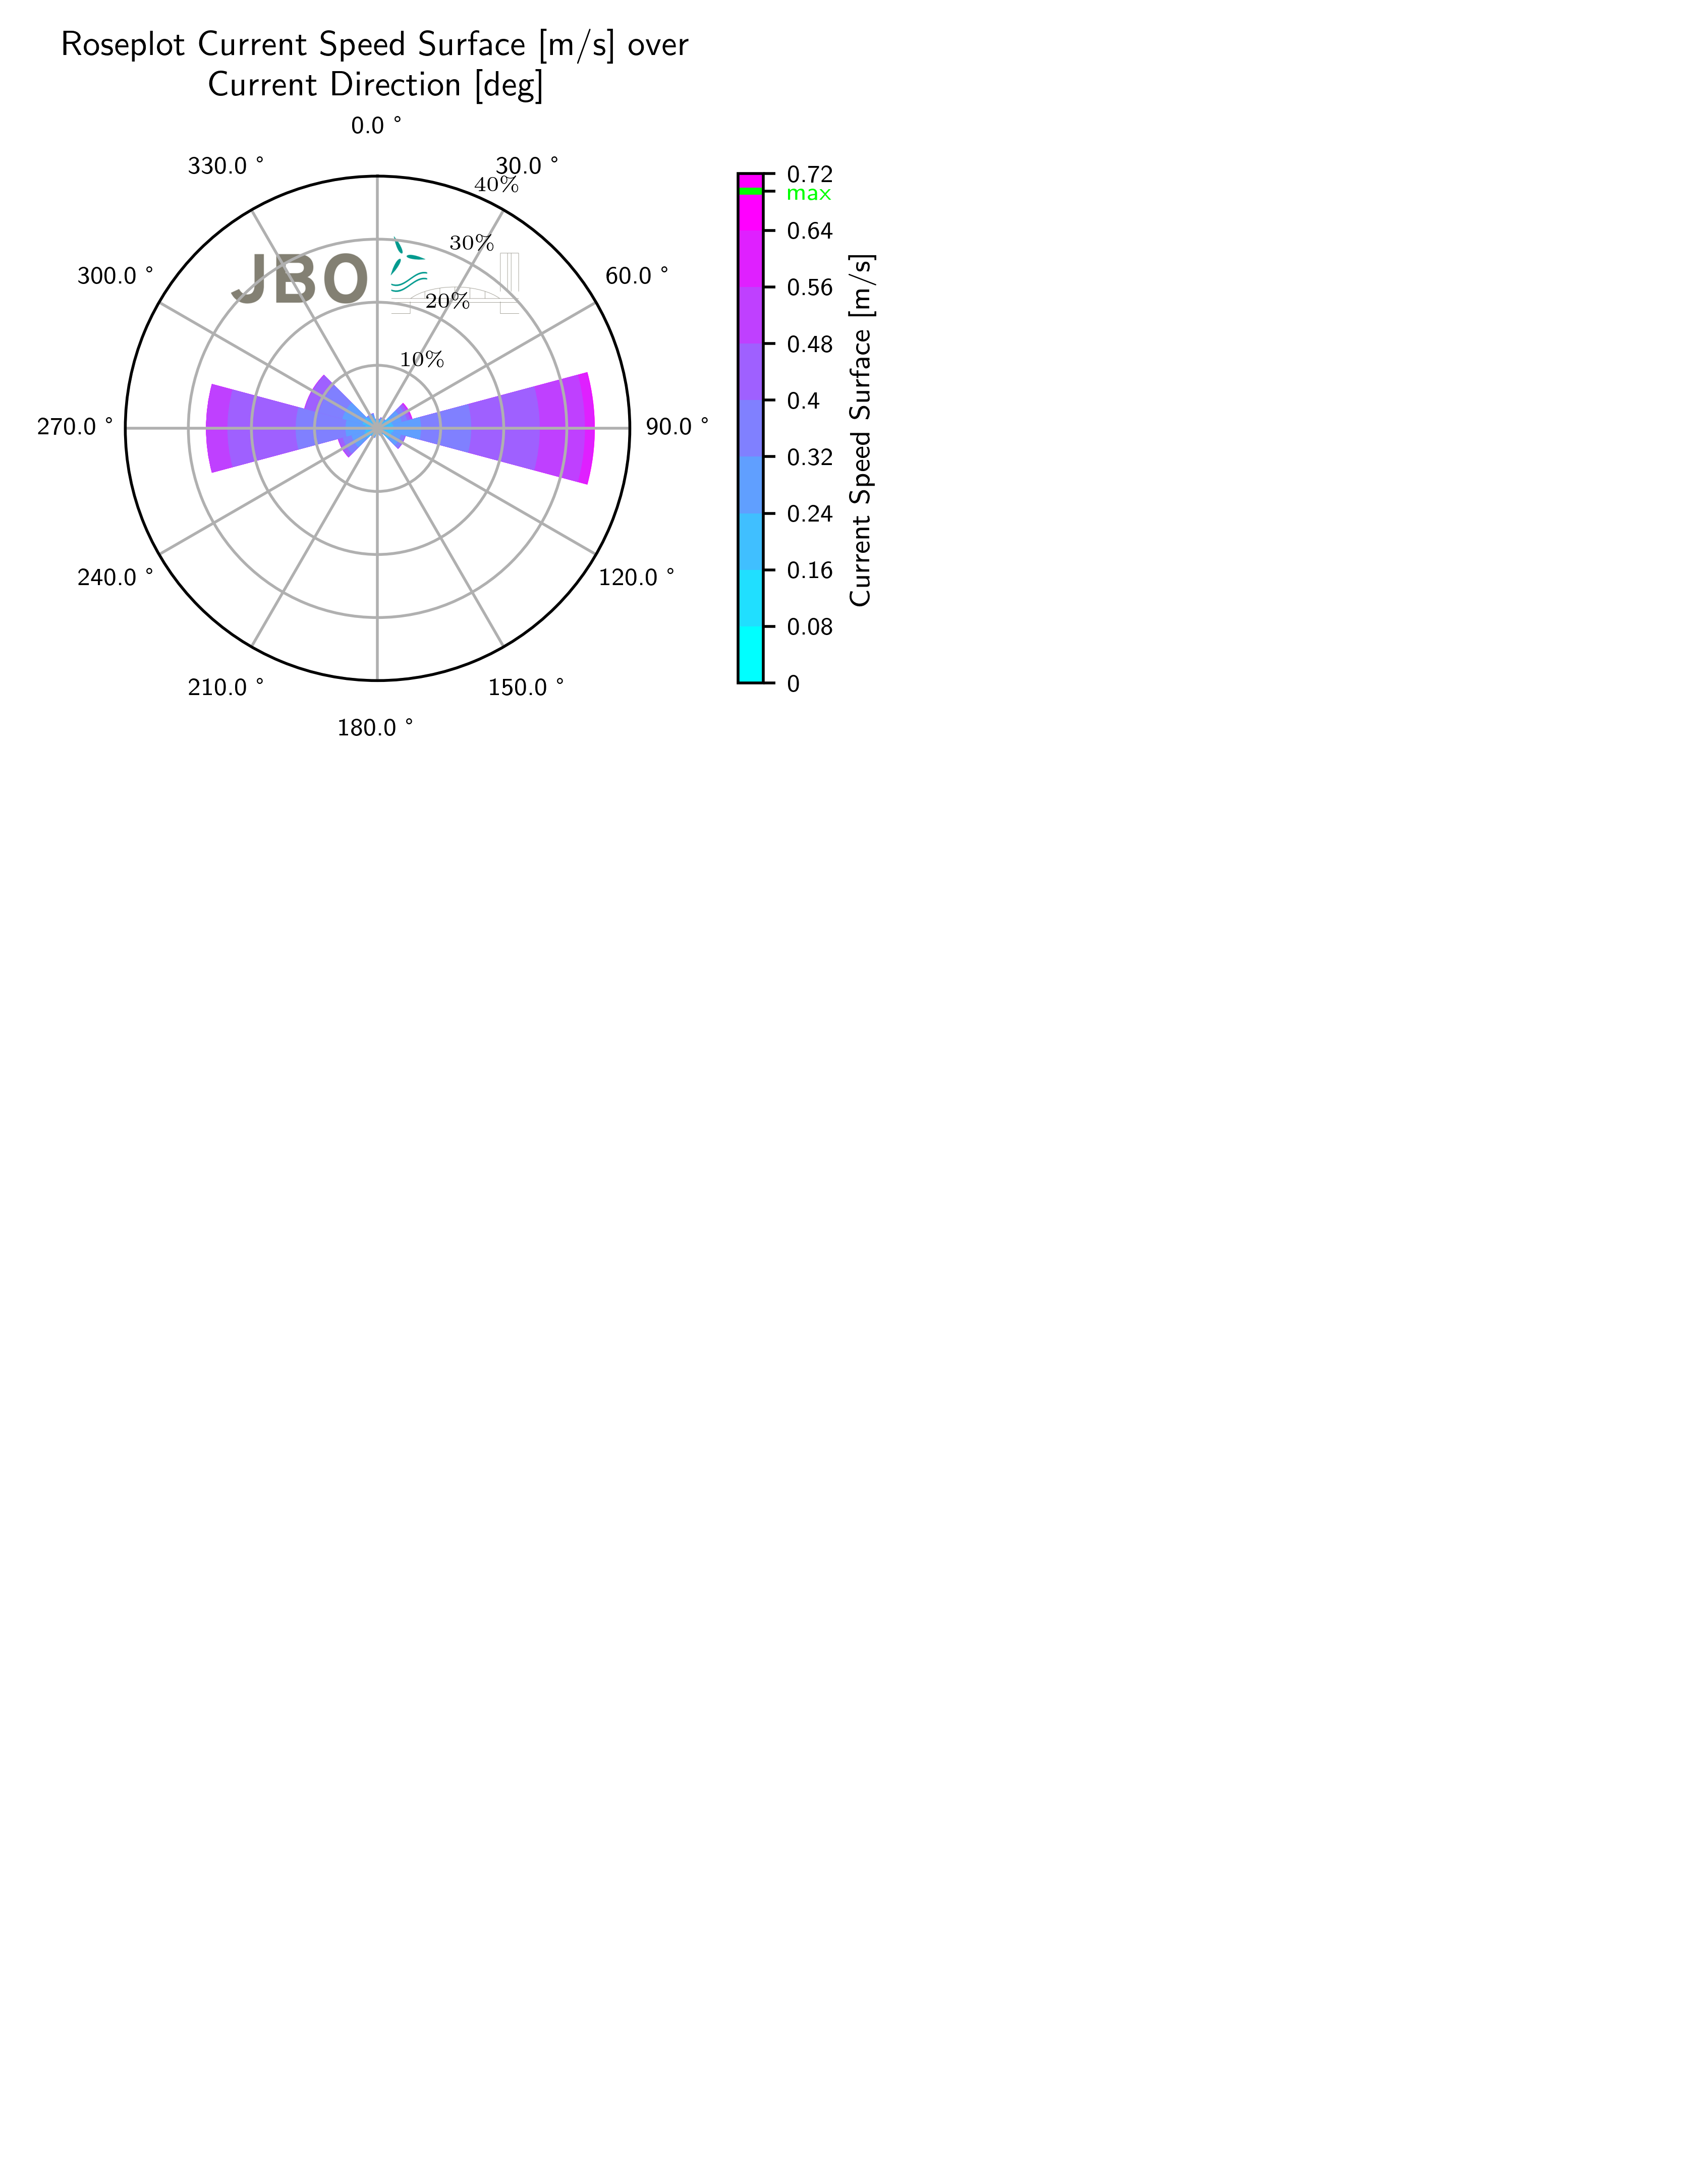
\includegraphics[width=1.0\textwidth]{C:/Users/aaron.lange/Desktop/Projekte/Hindcast_Tool/HindTool/example_output/Roseplots_currents_page_1.png} 
 \caption{ Roseplots-currents-page-1 } 
 \label{fig: Roseplots_currents_page_1 } 
\end{figure}
\section{Data correlation and interpretation}
\subsection{Normal Sea State}

Wind speed dependent omnidirectional and directional normal sea state parameter significant wave height and peak/zero crossing period are evaluated. Based on the joint occurrences of wind speed and significant wave height, and wave period and significant wave height, sensor correlations are developed.

As monopiles are sensitive to wave excitation, a methodology shall be applied to derive sea state parameters for the wave load generation in the most accurate way. Wave loading has two effects on design loads:

\begin{itemize}
  \item Quasi-static contribution: Wave loads on individual members do have a quasi-static effect, i.e. the wave loads result in internal member forces. Quasi-static fatigue loads can be assumed to be proportional to $\mathrm{H}_{\mathrm{s}}{ }^{\lambda}$, where $\lambda$ is 1 if the wave loading is inertia dominated and 2 if the wave loading is drag dominated [L2].
  \item Energy conservation: In order to maintain the wave energy of the measured/modelled sea states it is considered that $E \sim \mathrm{H}_{\mathrm{s}}{ }^{2}$.
  \item Dynamic contribution: In addition to the (local) quasi-static contribution, global dynamic excitation occurs. For monopiles this is the dominant effect. For stiff structures, such as jackets, this effect may be negligible. The most probable peak periods will be applied in the expected bandwidth of the first natural frequency ( $50 \%$-quantile), while the periods above and below this defined range are chosen to be on the slightly conservative side by means of different quantiles. See also section Fehler! Verweisquelle konnte nicht gefunden werden..
\end{itemize}

Weighting of the underlying hindcast data, provided in REF, can hence be performed in two stages:

\begin{itemize}
  \item An equivalent $H_{S}$ is found based on quasi-static and energy-conserving considerations.
  \item An equivalent $T_{P}$ is found based on dynamic aspects.
\end{itemize}

This ensures that both quasi-static and resonant contributions of the response are adequately covered.\\
The condensation process involves the following steps:\\
For each directional sector, the corresponding ordinate values $(y)$ over the abscissa values $(x)$ are considered based on the hindcast data. In case of wind speed to significant wave height condensation, $x$ represents the wind speed and $y$ represents the wave height. For significant wave height versus peak period, $x$ represents the wave height and $y$ represents the peak period.

Initially, the hindcast datapoints are sorted into several bins (see "bin number" in REF and REF). All bins have the same width in $x$. For each bin, a $y$ value is then calculated. This value can be determined by various methods: the arithmetic mean, the median or another quantile, or - in the case of $H_{S}$ - by the weighting approach specified in Eq. 6-2. The chosen method is indicated in "method to derive representative value" in Table 6-1 and Table 6-2. The derived values can subsequently be corrected ("correction factor on averaged values" in Table 6-1). This correction is applied by adjusting the $H_{S}$ values if the DEL comparison between the condensation method and the hindcast data yields unsatisfactory results. This comparison is detailed in section Fehler! Verweisquelle konnte nicht gefunden werden.. The final $y$ values for each bin are referred to as the representative value of each bin.

\begin{figure}[H] 
 \centering 
 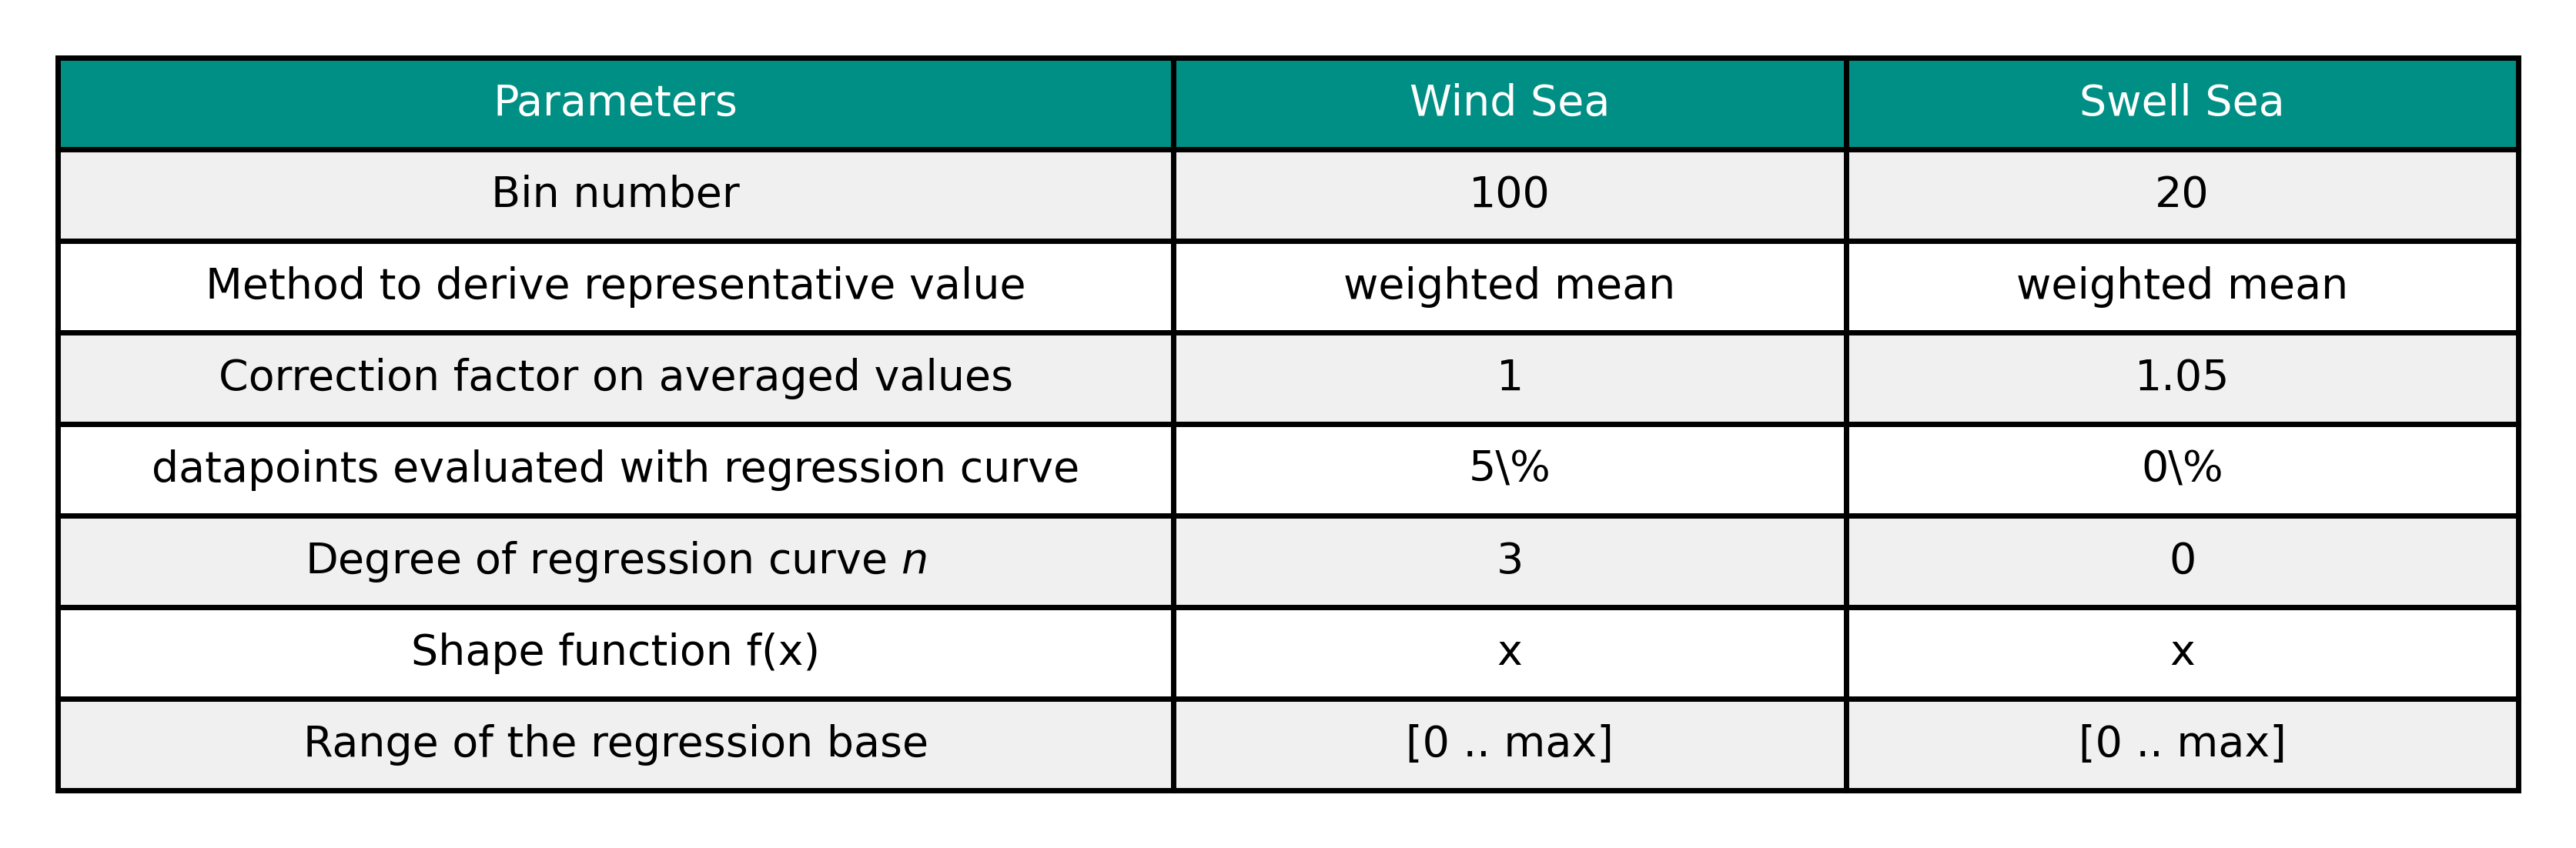
\includegraphics[width=1.0\textwidth ]{C:/Users/aaron.lange/Desktop/Projekte/Hindcast_Tool/HindTool/example_output/Report_table_VMHS_page_1.png} 
 \captionsetup{type=table} 
\caption{ Report-table-VMHS-page-1 } 
 \label{tab: Report_table_VMHS_page_1 } 
\end{figure}

For higher wind speeds and wave heights, the number of datapoints in the hindcast data set decreases. This can lead to representative values for higher bins fluctuating. To mitigate this, a regression analysis is performed. The results from the regression analysis are then used for the higher bins instead of the representative values. The parameter "proportion of datapoints evaluated with regression curve" (Table 6-1 and Table 6-2) specifies how many points of the hindcast set are considered using the regression analysis results rather than the representative values of the bins. The regression analysis is based on a polynomial function of degree $n$ (defined in Table 6-1 and Table 6-2):

$$
\hat{y}(x)=\sum_{i=0}^{n} c_{i} f(x)^{i}
$$

The $x$ values represent either the wind speed (in case of the wind speed to significant wave height condensation) or the wave height (for significant wave height versus peak period) of each bin within the "range of the regression base" (see Table 6-1 and Table 6-2). $\hat{y}$ is the calculated wave height or peak period, respectively. The regression coefficients $c_{\mathrm{i}}$ are determined using a least-squares fit, which minimizes the deviations of $\hat{y}$ to the calculated representative value of each bin. The function $f(x)$ is typically either $x$ or $\sqrt{x}$ and is specified in Table 6-1 and Table 6-2.

Finally, the selected condensation values are a combination of the representative values for the first bins and the values calculated by the regression curve for the higher bins. Note that a regression curve is not always necessary. In such cases, the parameter "proportion of datapoints evaluated with regression curve (highest wind speeds)" is $0 \%$, and all condensation results are derived from the representative values.



\subsubsection{Significant wave height over wind speed}
An equivalent significant wave height vs. wind speed correlation is determined for the omnidirectional case and the directional distribution. The following weighting approach is applied:

$$
H_{s, e q}=\left(\frac{\sum_{n} H_{s, n}{ }^{\lambda m} \cdot p(n)}{\sum_{n} p(n)}\right)^{\frac{1}{\lambda m}}
$$

Here, $\lambda$ is chosen to be 1 as wave loads on monopiles are inertia dominated (see also [L2]), whereas $m$ shall be equal to 2 and denotes the power mean exponent. This approach is solely based on the conservation of the wave energy of a sea state or the corresponding spectrum, respectively. The wave energy of a linear sea state is proportional to the square of significant wave height $\left(E \sim H_{S}^{2}\right)$.

The calculated condensation curve is adjusted to ensure it forms a monotone increasing function. This means that as wind speeds increase, the $H_{S}$ either increases or remains constant. This is physically obvious but can be calculated differently for high bins due to a lack of data.

The condensation is calculated using the following parameters in REF.\\
REF: Condensation parameter wind speed versus significant wave height
 
\begin{figure}[H] 
 \centering 
 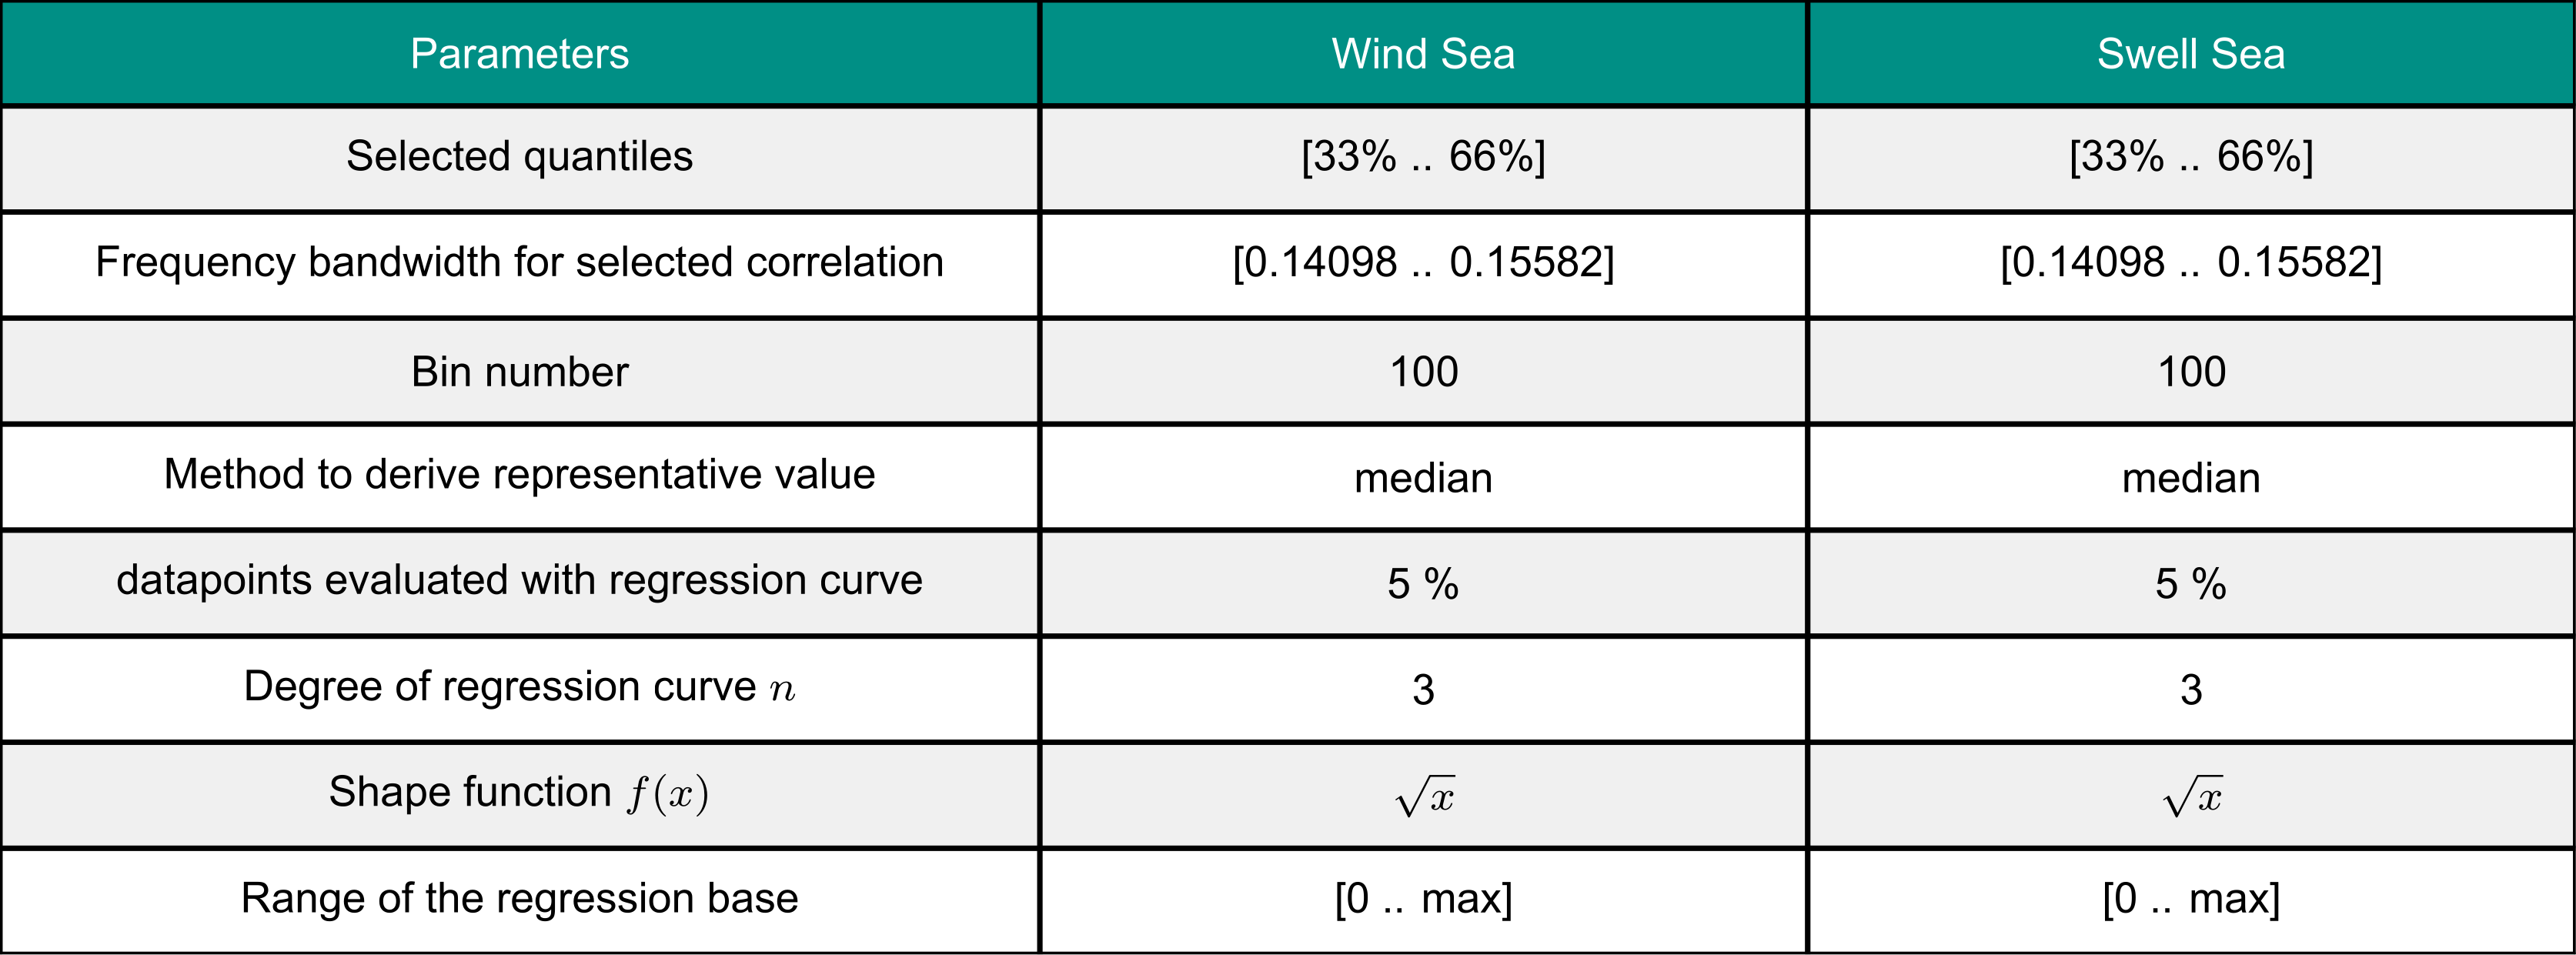
\includegraphics[width=1.0\textwidth ]{C:/Users/aaron.lange/Desktop/Projekte/Hindcast_Tool/HindTool/example_output/Report_table_HSTP_page_1.png} 
 \captionsetup{type=table} 
\caption{ Report-table-HSTP-page-1 } 
 \label{tab: Report_table_HSTP_page_1 } 
\end{figure}

The result for the omnidirectional wind sea case is shown REF. Results for each sector are listed in Fehler! Verweisquelle konnte nicht gefunden werden.\\
omnidirectional\\

\begin{figure}[H] 
 \centering 
 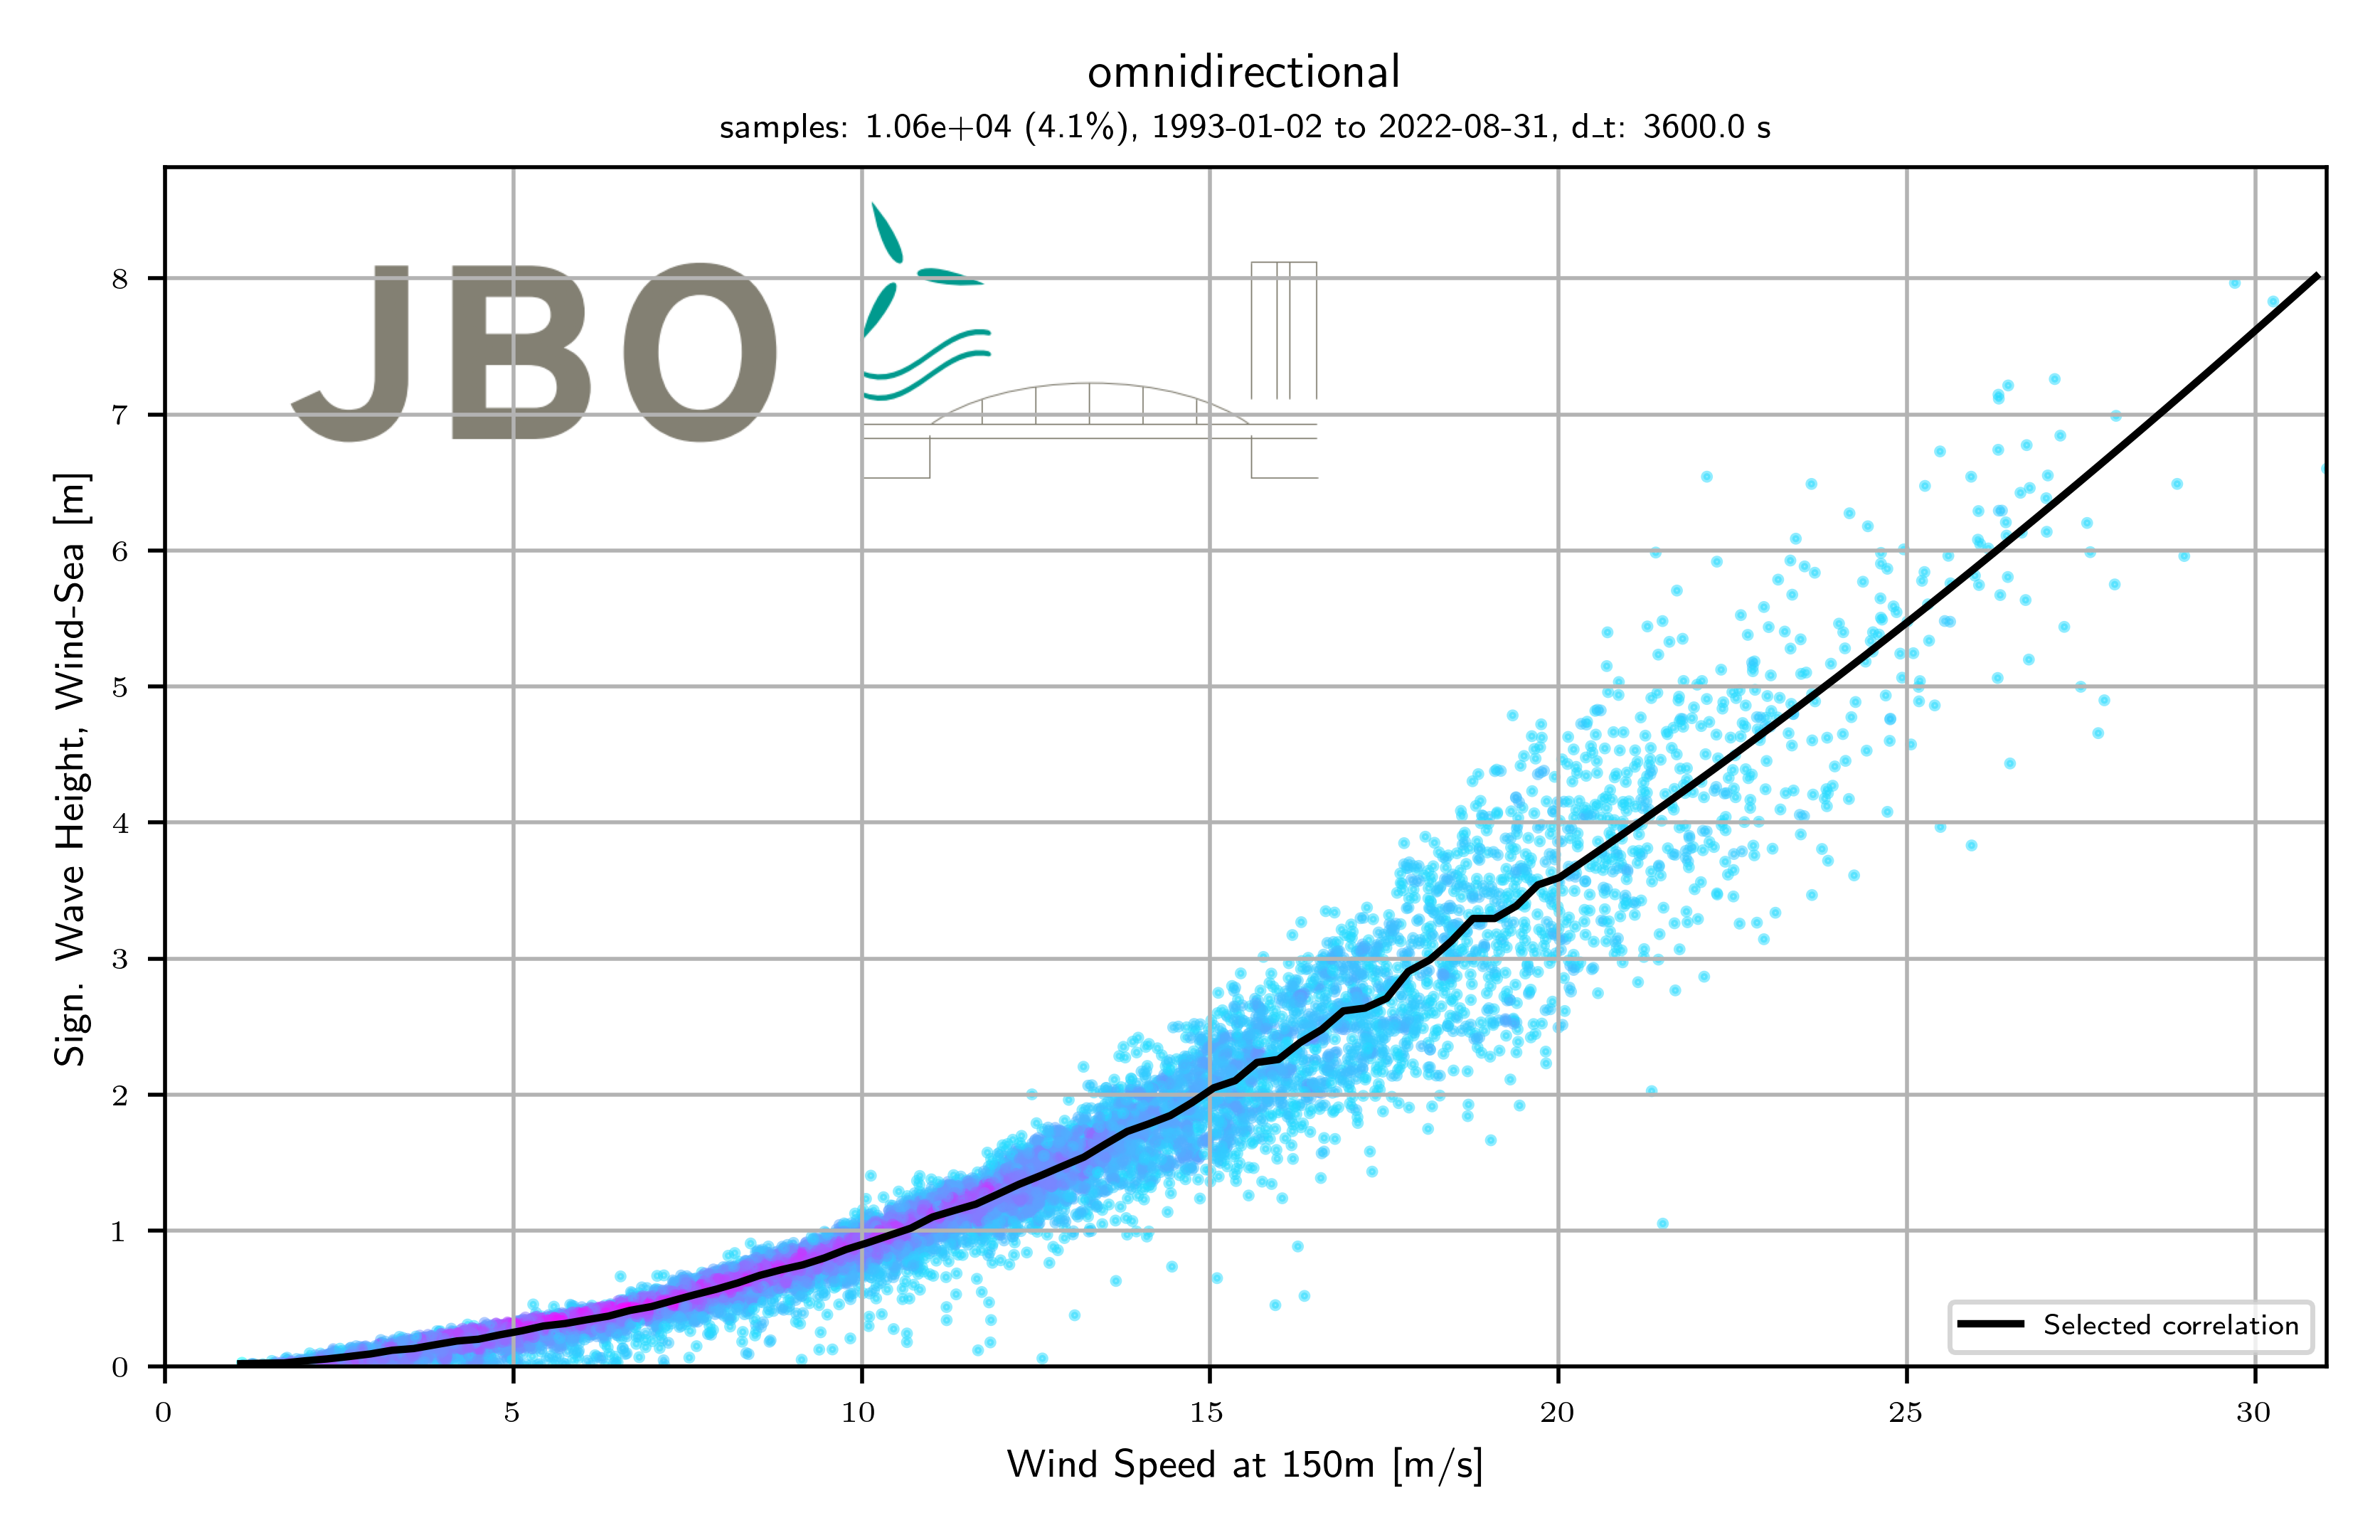
\includegraphics[width=1.0\textwidth]{C:/Users/aaron.lange/Desktop/Projekte/Hindcast_Tool/HindTool/example_output/VMHS_wind_page_3.png} 
 \caption{ VMHS-wind-page-3 } 
 \label{fig: VMHS_wind_page_3 } 
\end{figure}
\begin{figure}[H] 
 \centering 
 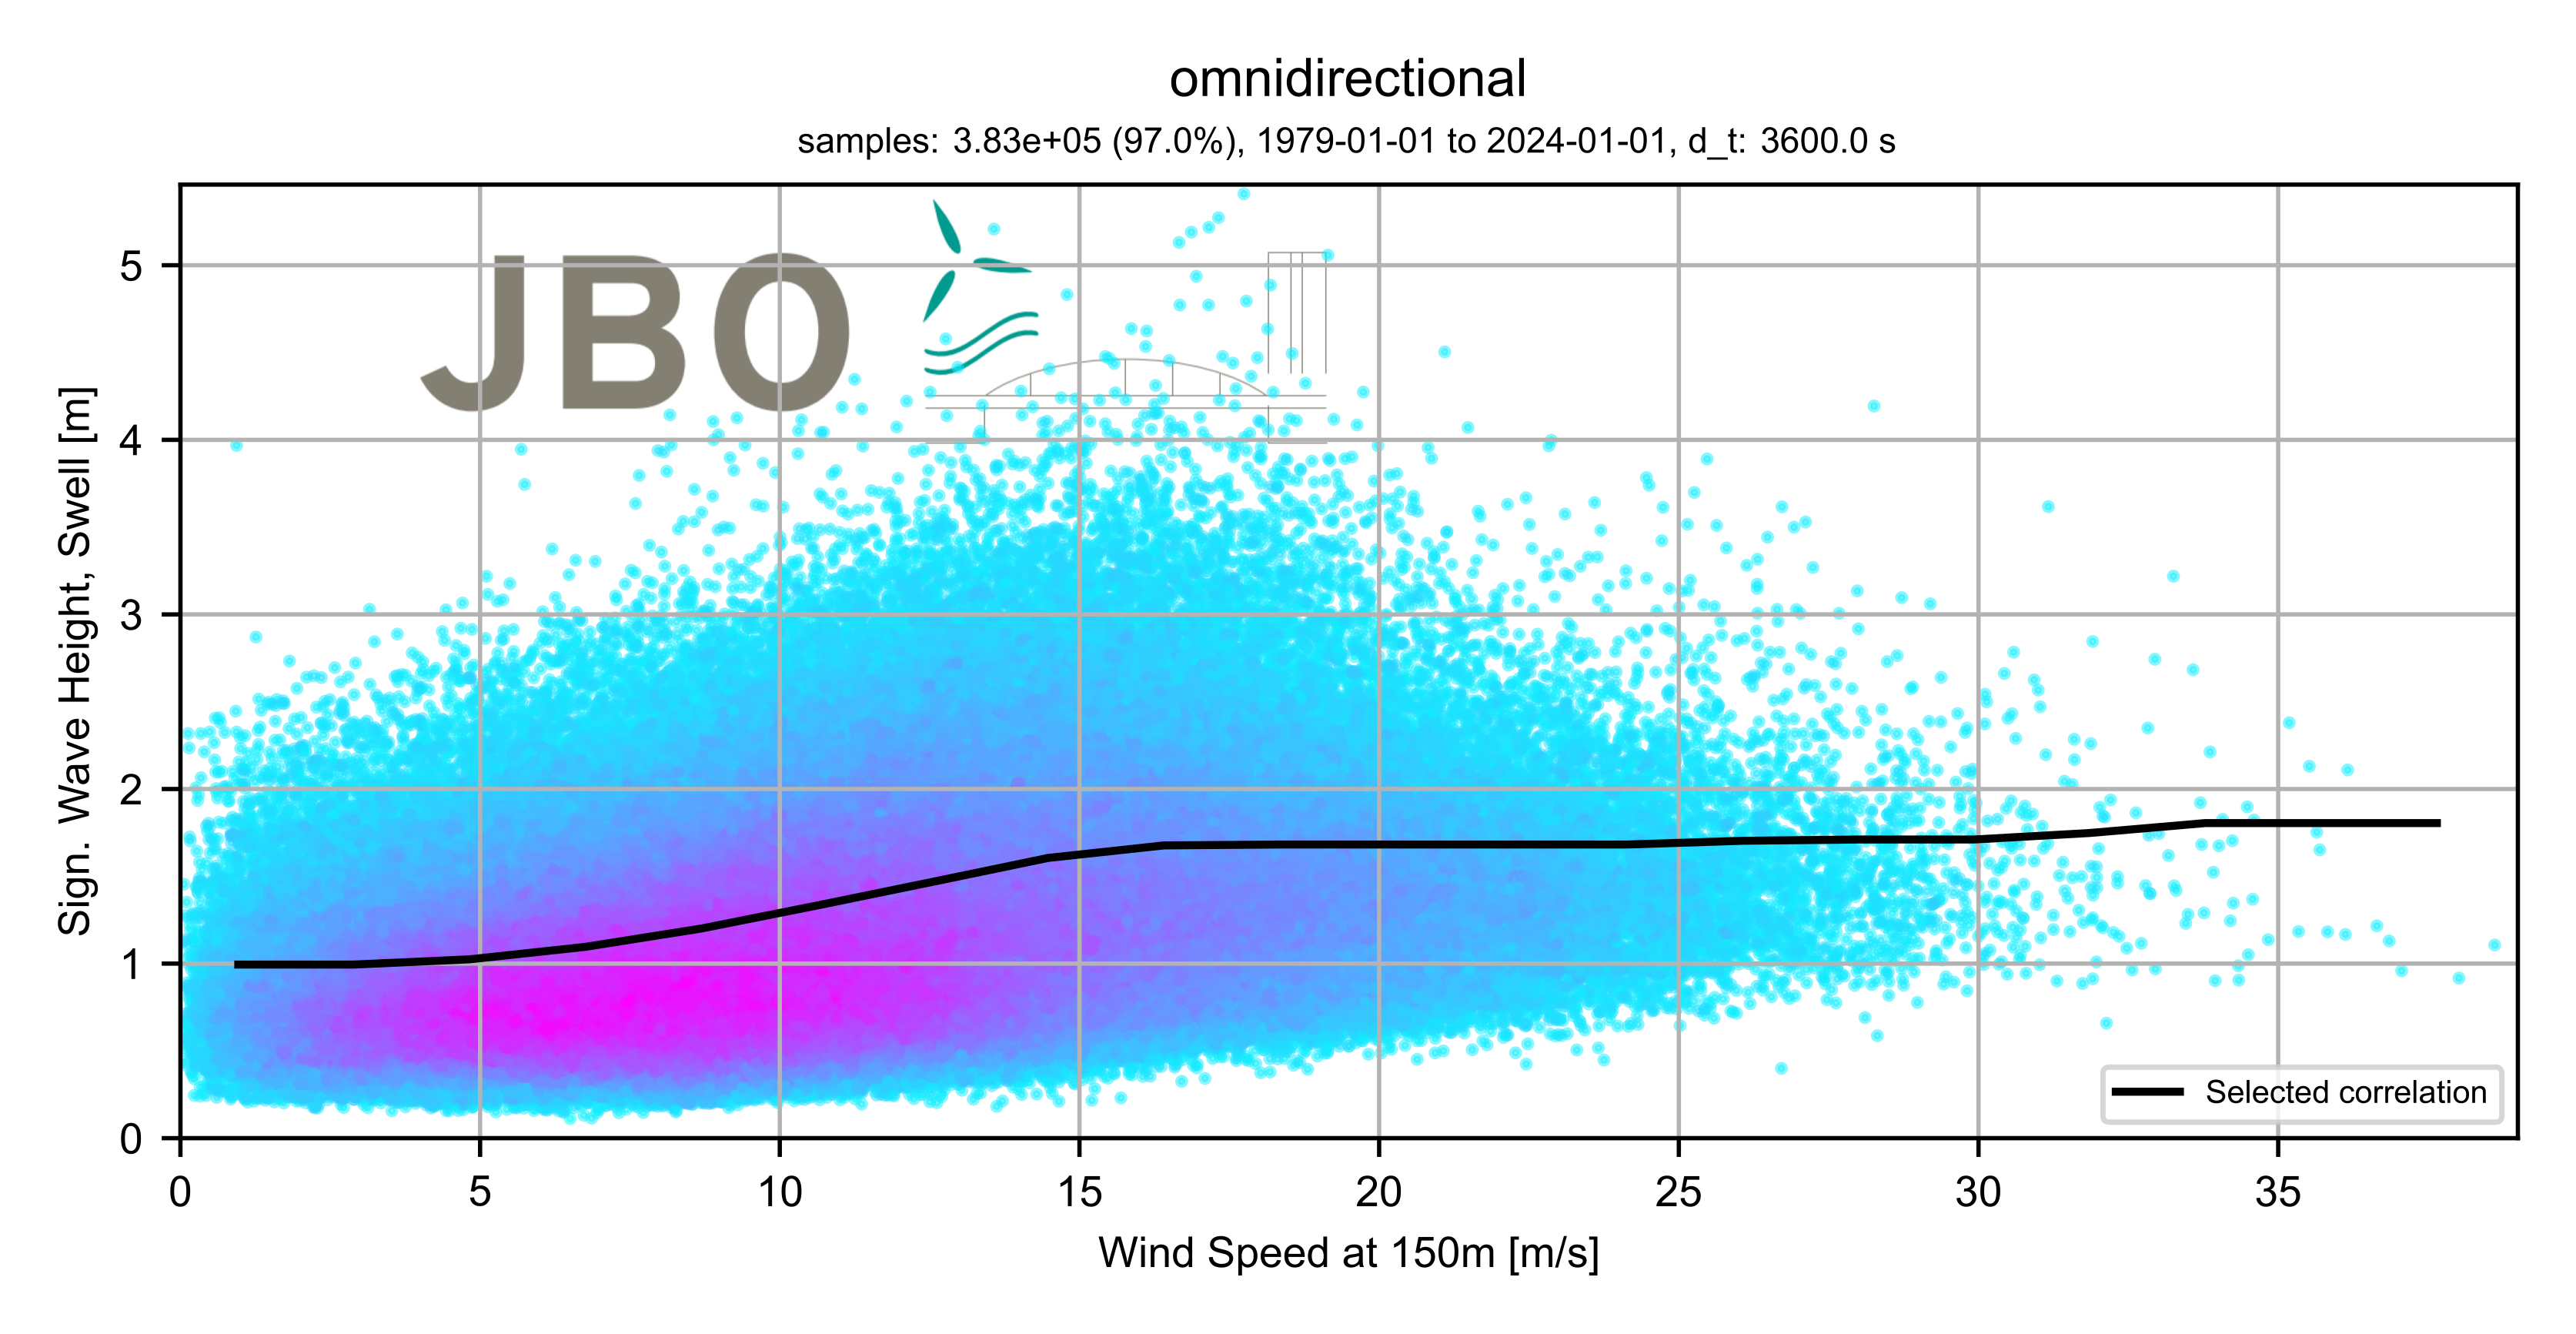
\includegraphics[width=1.0\textwidth]{C:/Users/aaron.lange/Desktop/Projekte/Hindcast_Tool/HindTool/example_output/VMHS_swell_page_3.png} 
 \caption{ VMHS-swell-page-3 } 
 \label{fig: VMHS_swell_page_3 } 
\end{figure}

\begin{figure}[H] 
 \centering 
 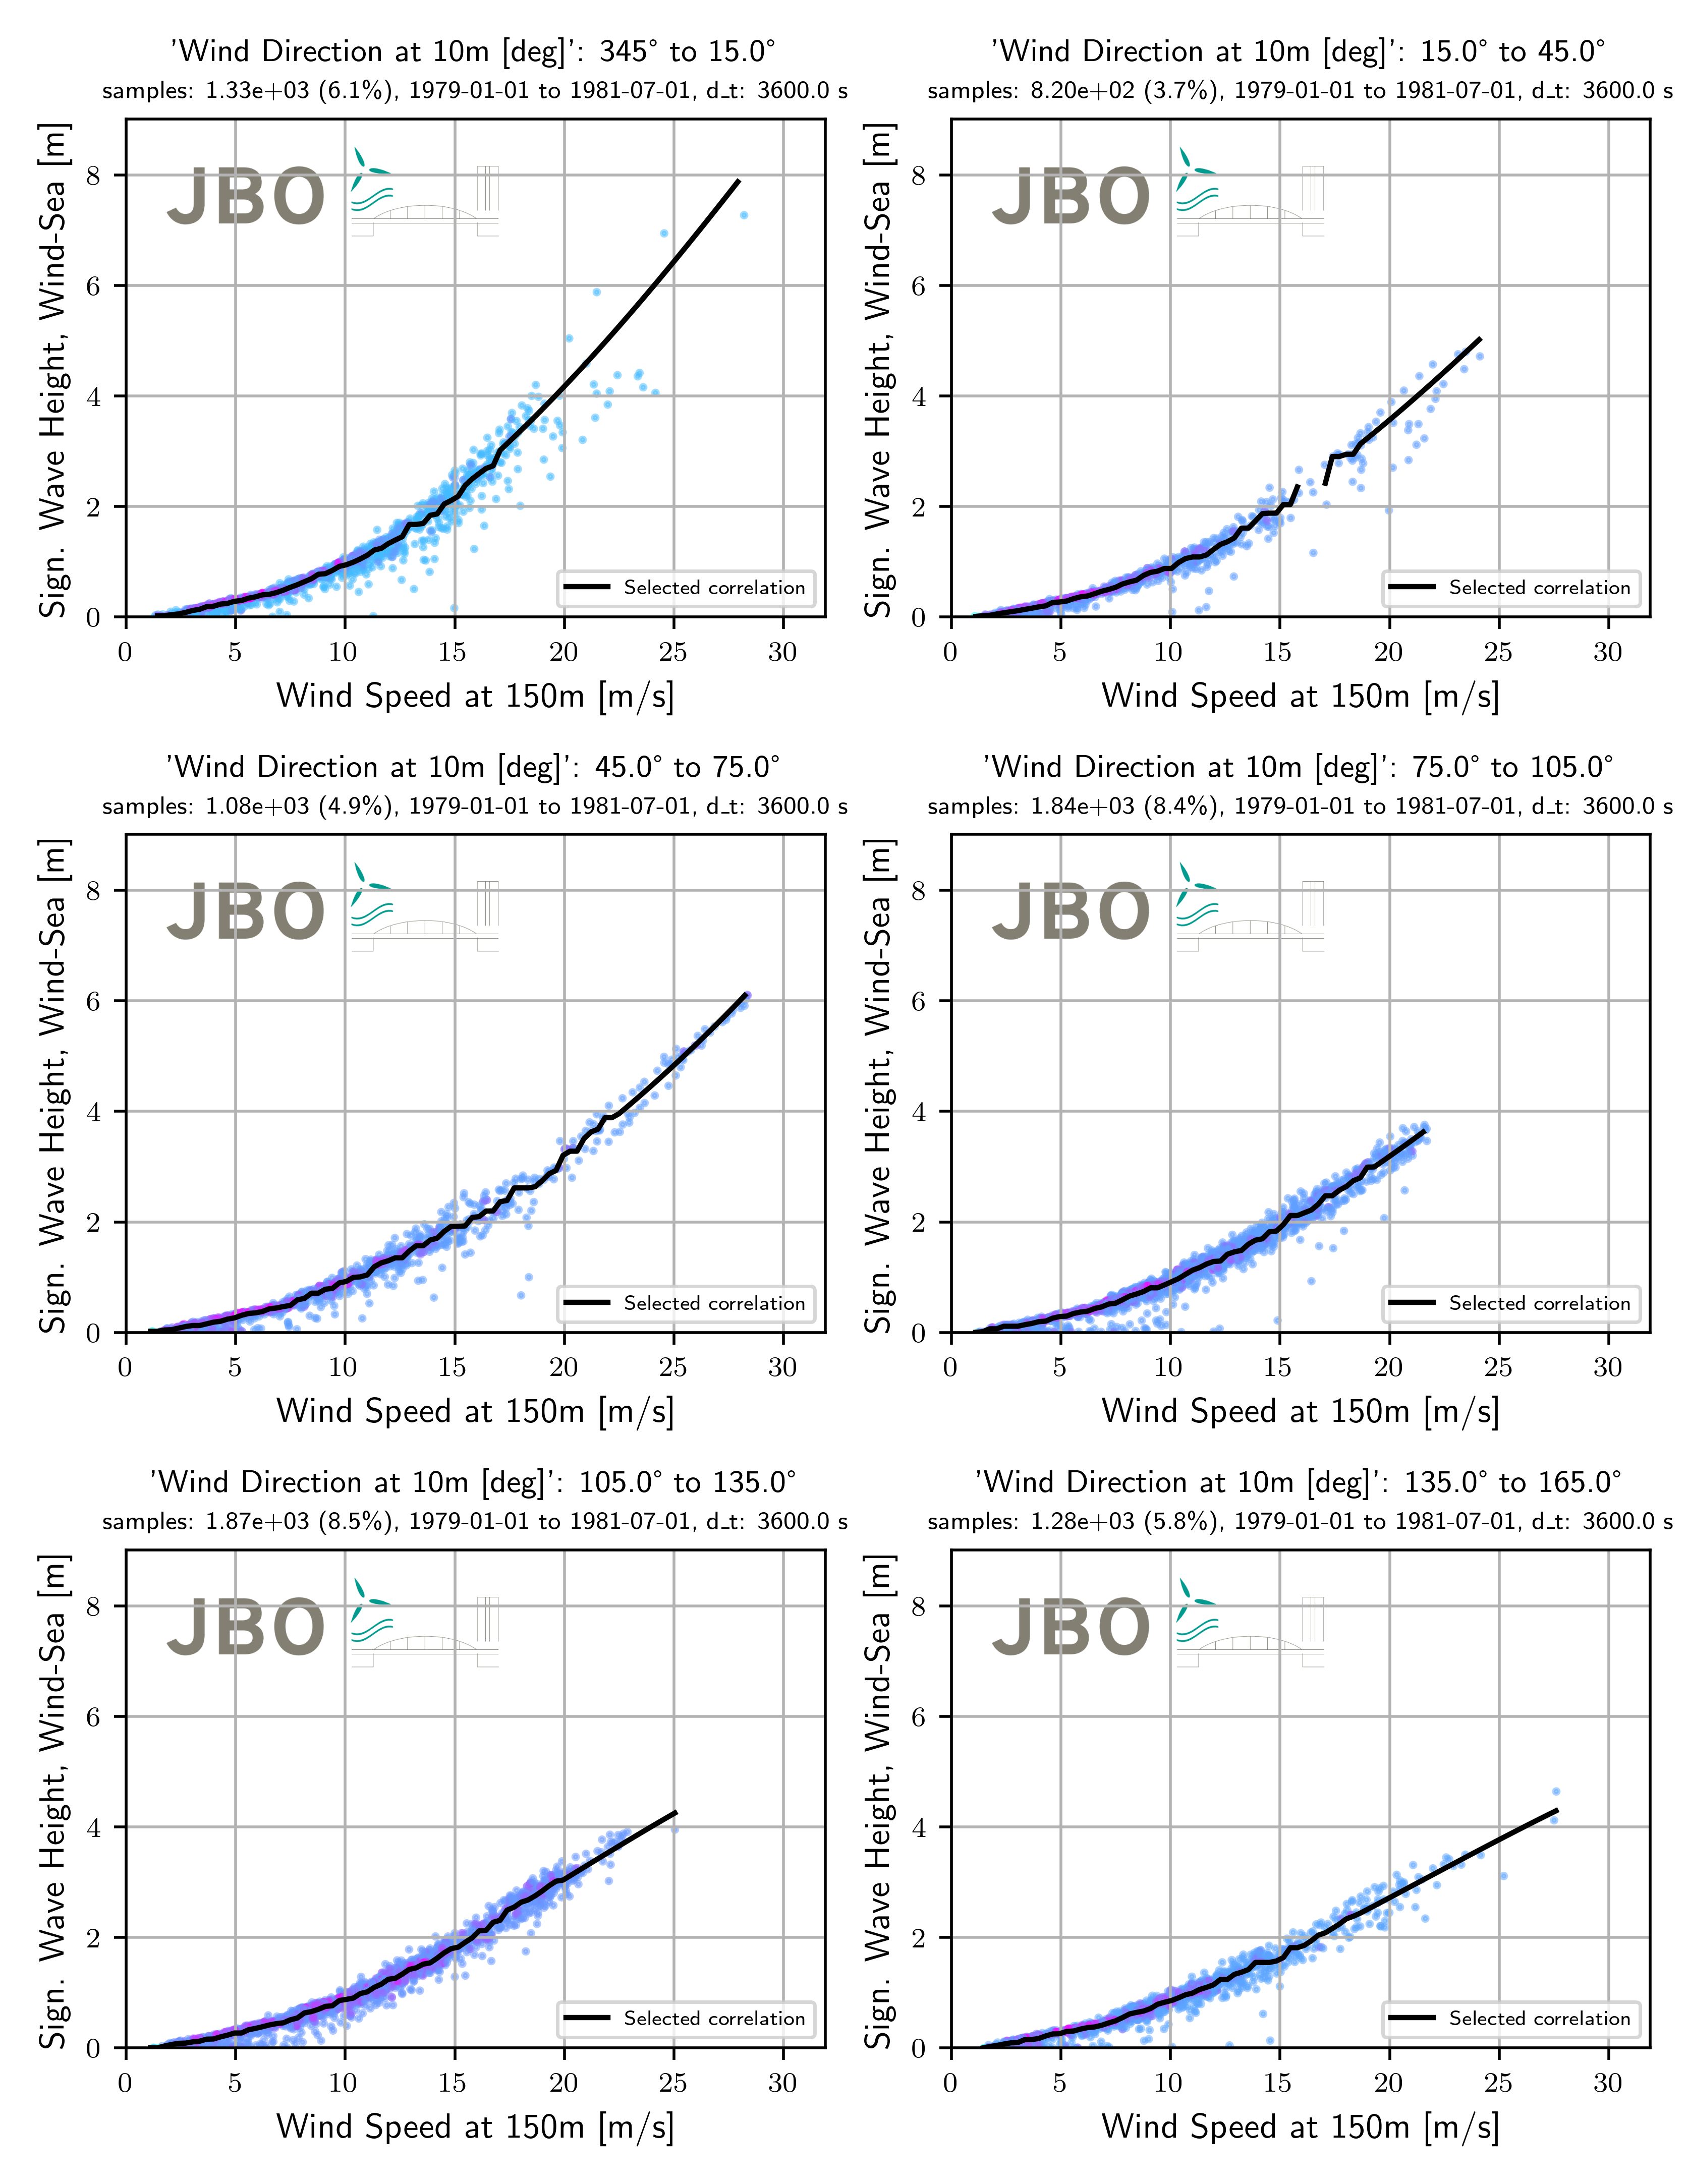
\includegraphics[width=1.0\textwidth]{C:/Users/aaron.lange/Desktop/Projekte/Hindcast_Tool/HindTool/example_output/VMHS_wind_page_1.png} 
 \caption{ VMHS-wind-page-1 } 
 \label{fig: VMHS_wind_page_1 } 
\end{figure}
\begin{figure}[H] 
 \centering 
 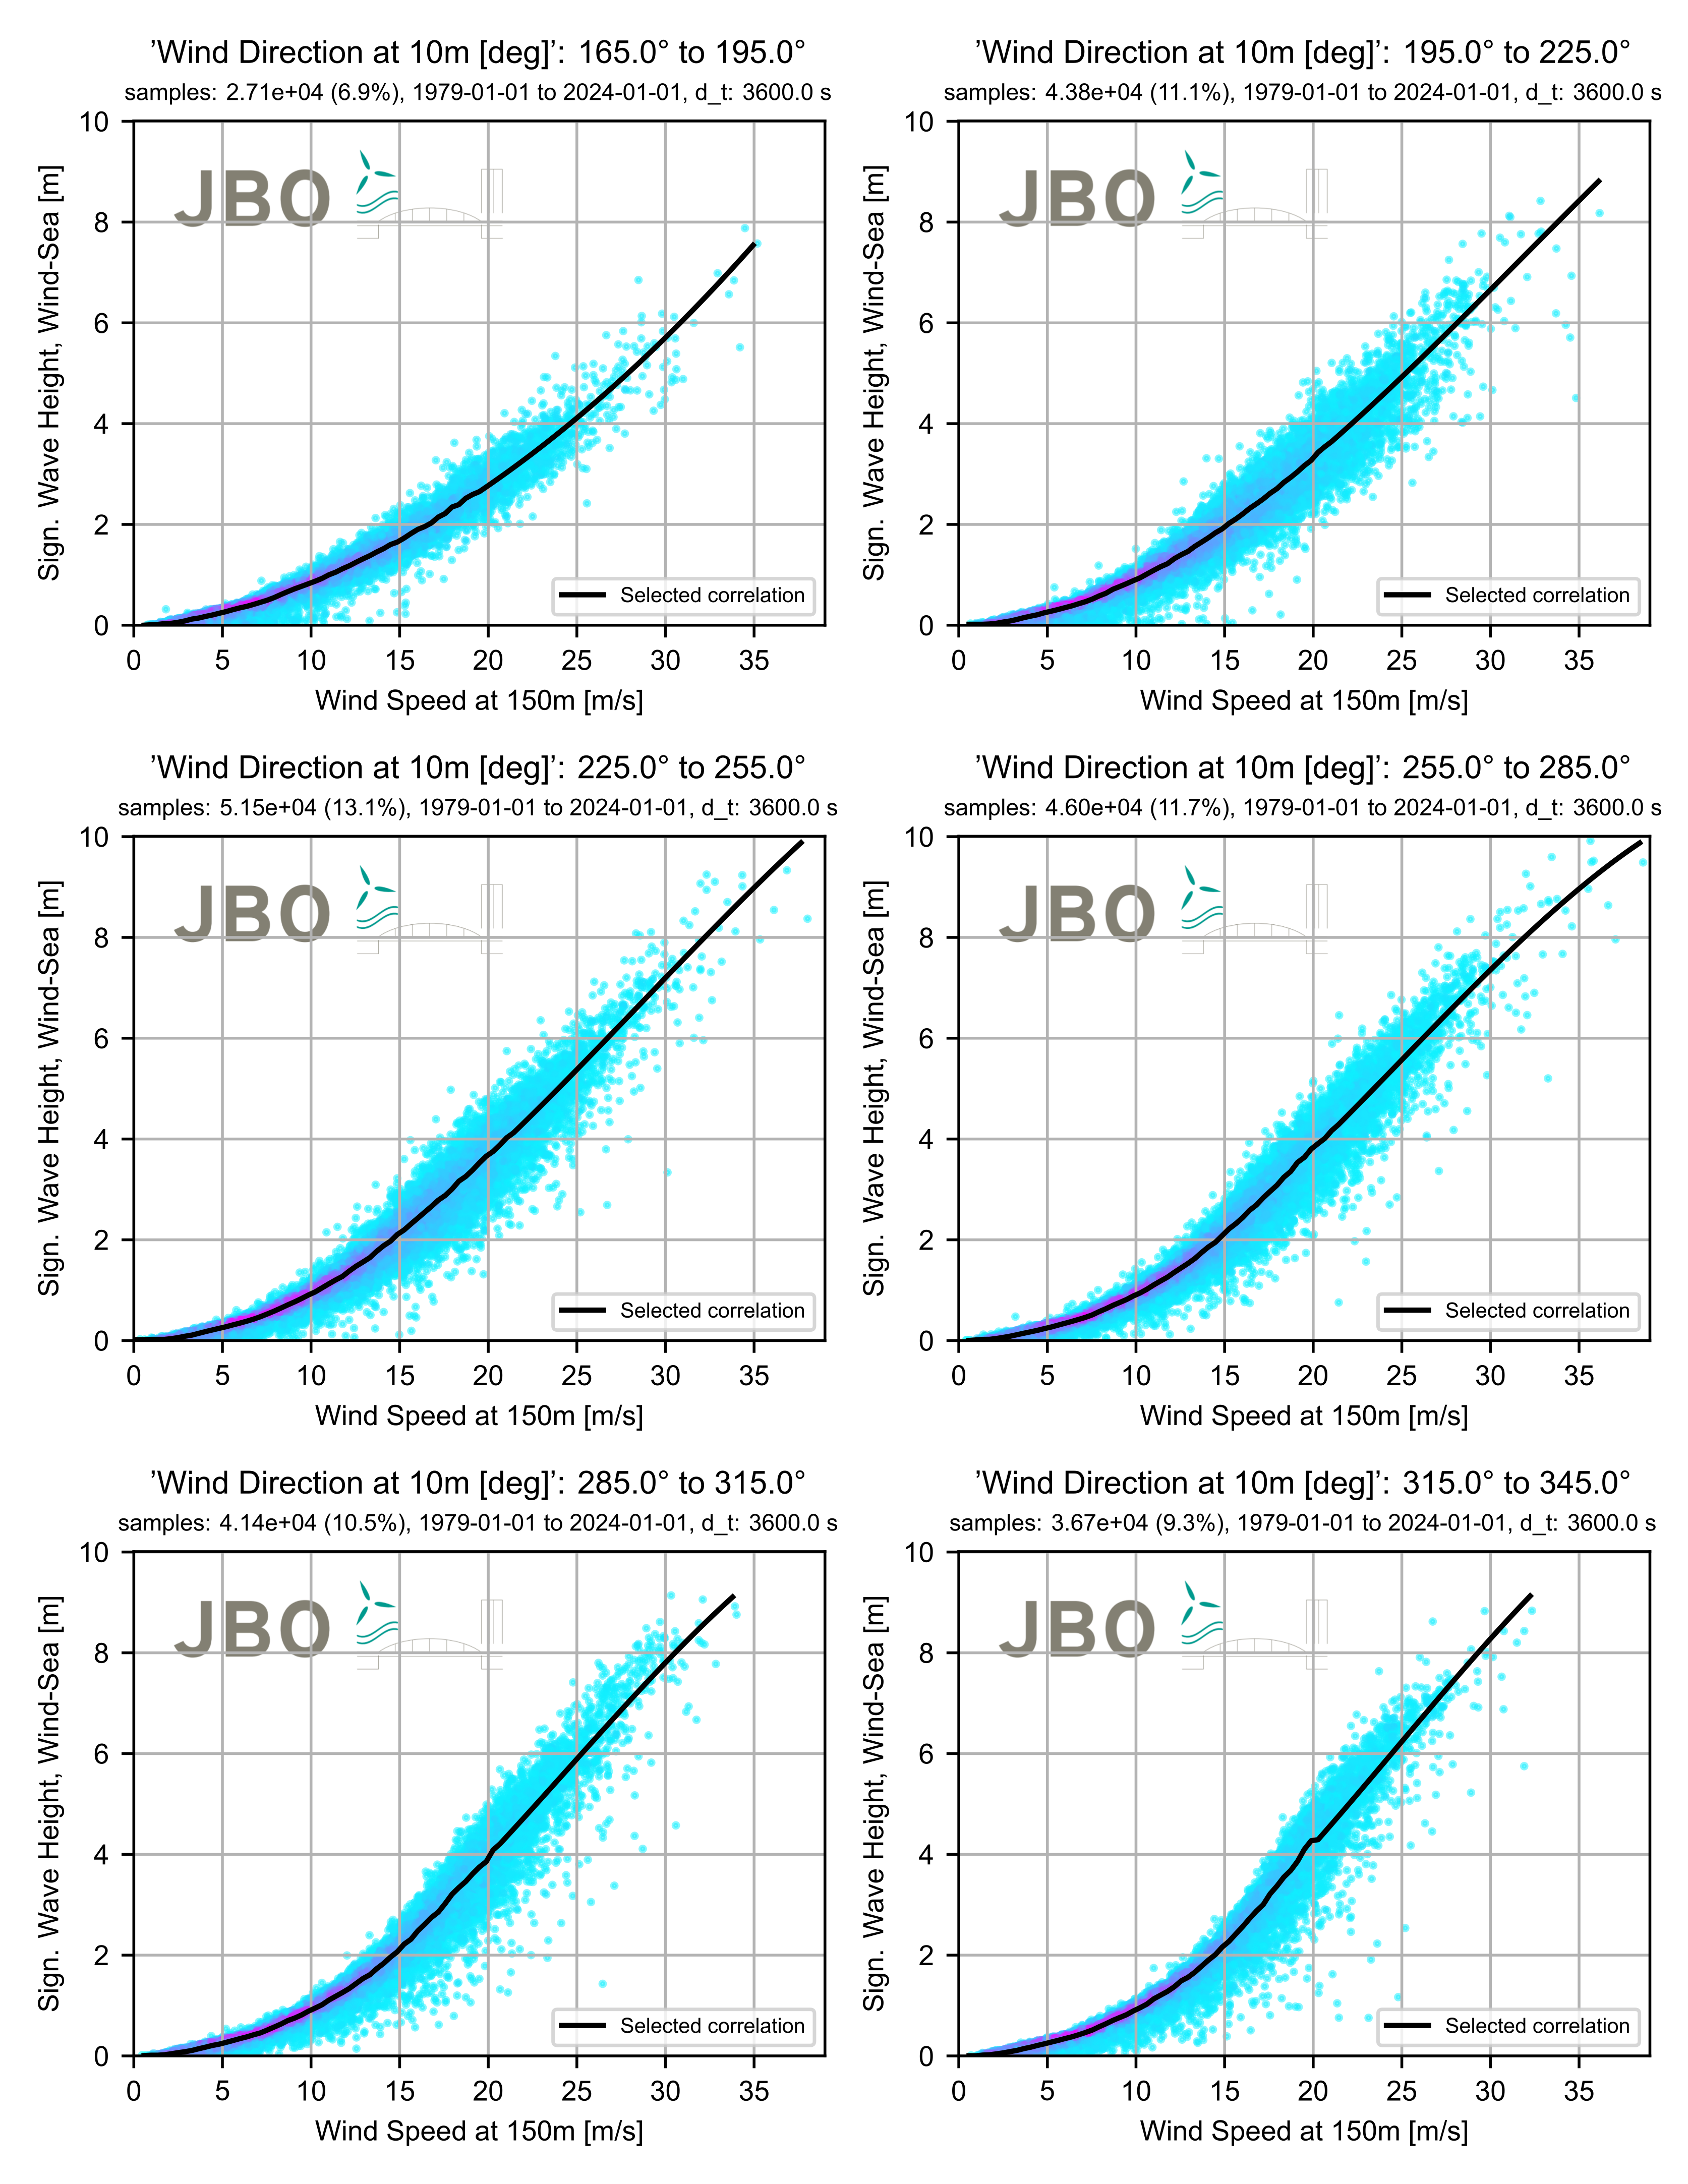
\includegraphics[width=1.0\textwidth]{C:/Users/aaron.lange/Desktop/Projekte/Hindcast_Tool/HindTool/example_output/VMHS_wind_page_2.png} 
 \caption{ VMHS-wind-page-2 } 
 \label{fig: VMHS_wind_page_2 } 
\end{figure}

\begin{figure}[H] 
 \centering 
 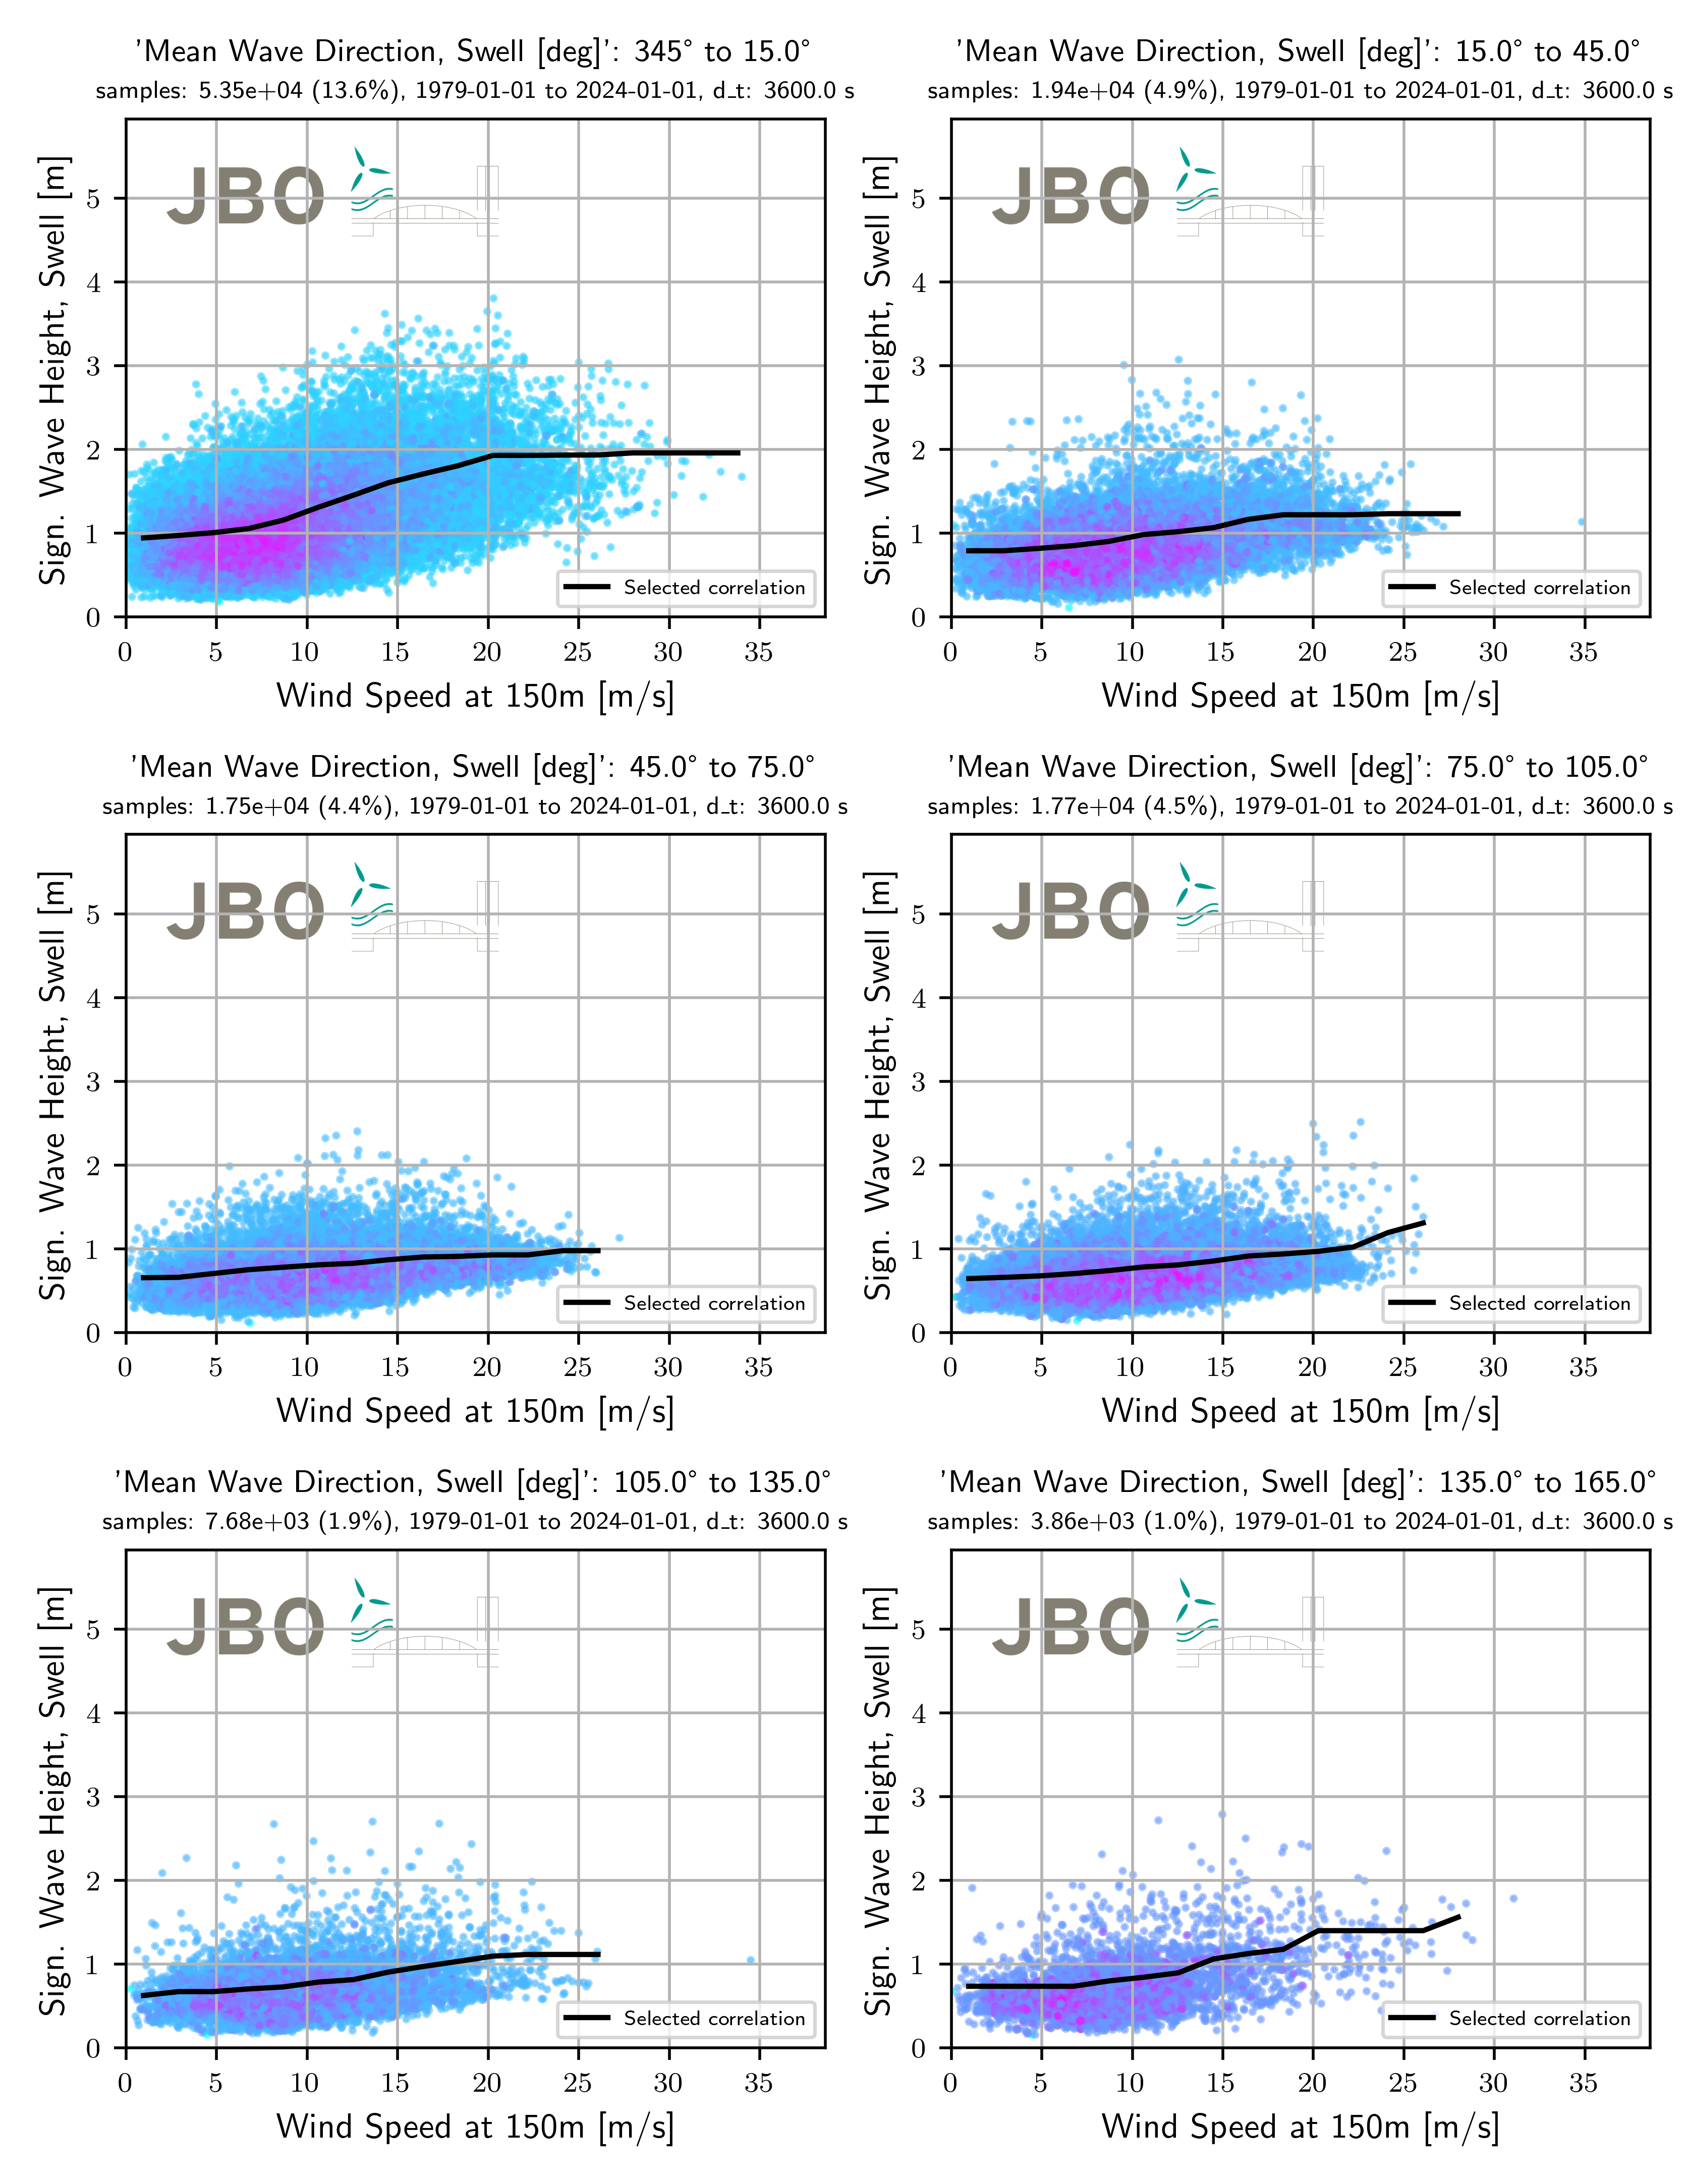
\includegraphics[width=1.0\textwidth]{C:/Users/aaron.lange/Desktop/Projekte/Hindcast_Tool/HindTool/example_output/VMHS_swell_page_1.png} 
 \caption{ VMHS-swell-page-1 } 
 \label{fig: VMHS_swell_page_1 } 
\end{figure}
\begin{figure}[H] 
 \centering 
 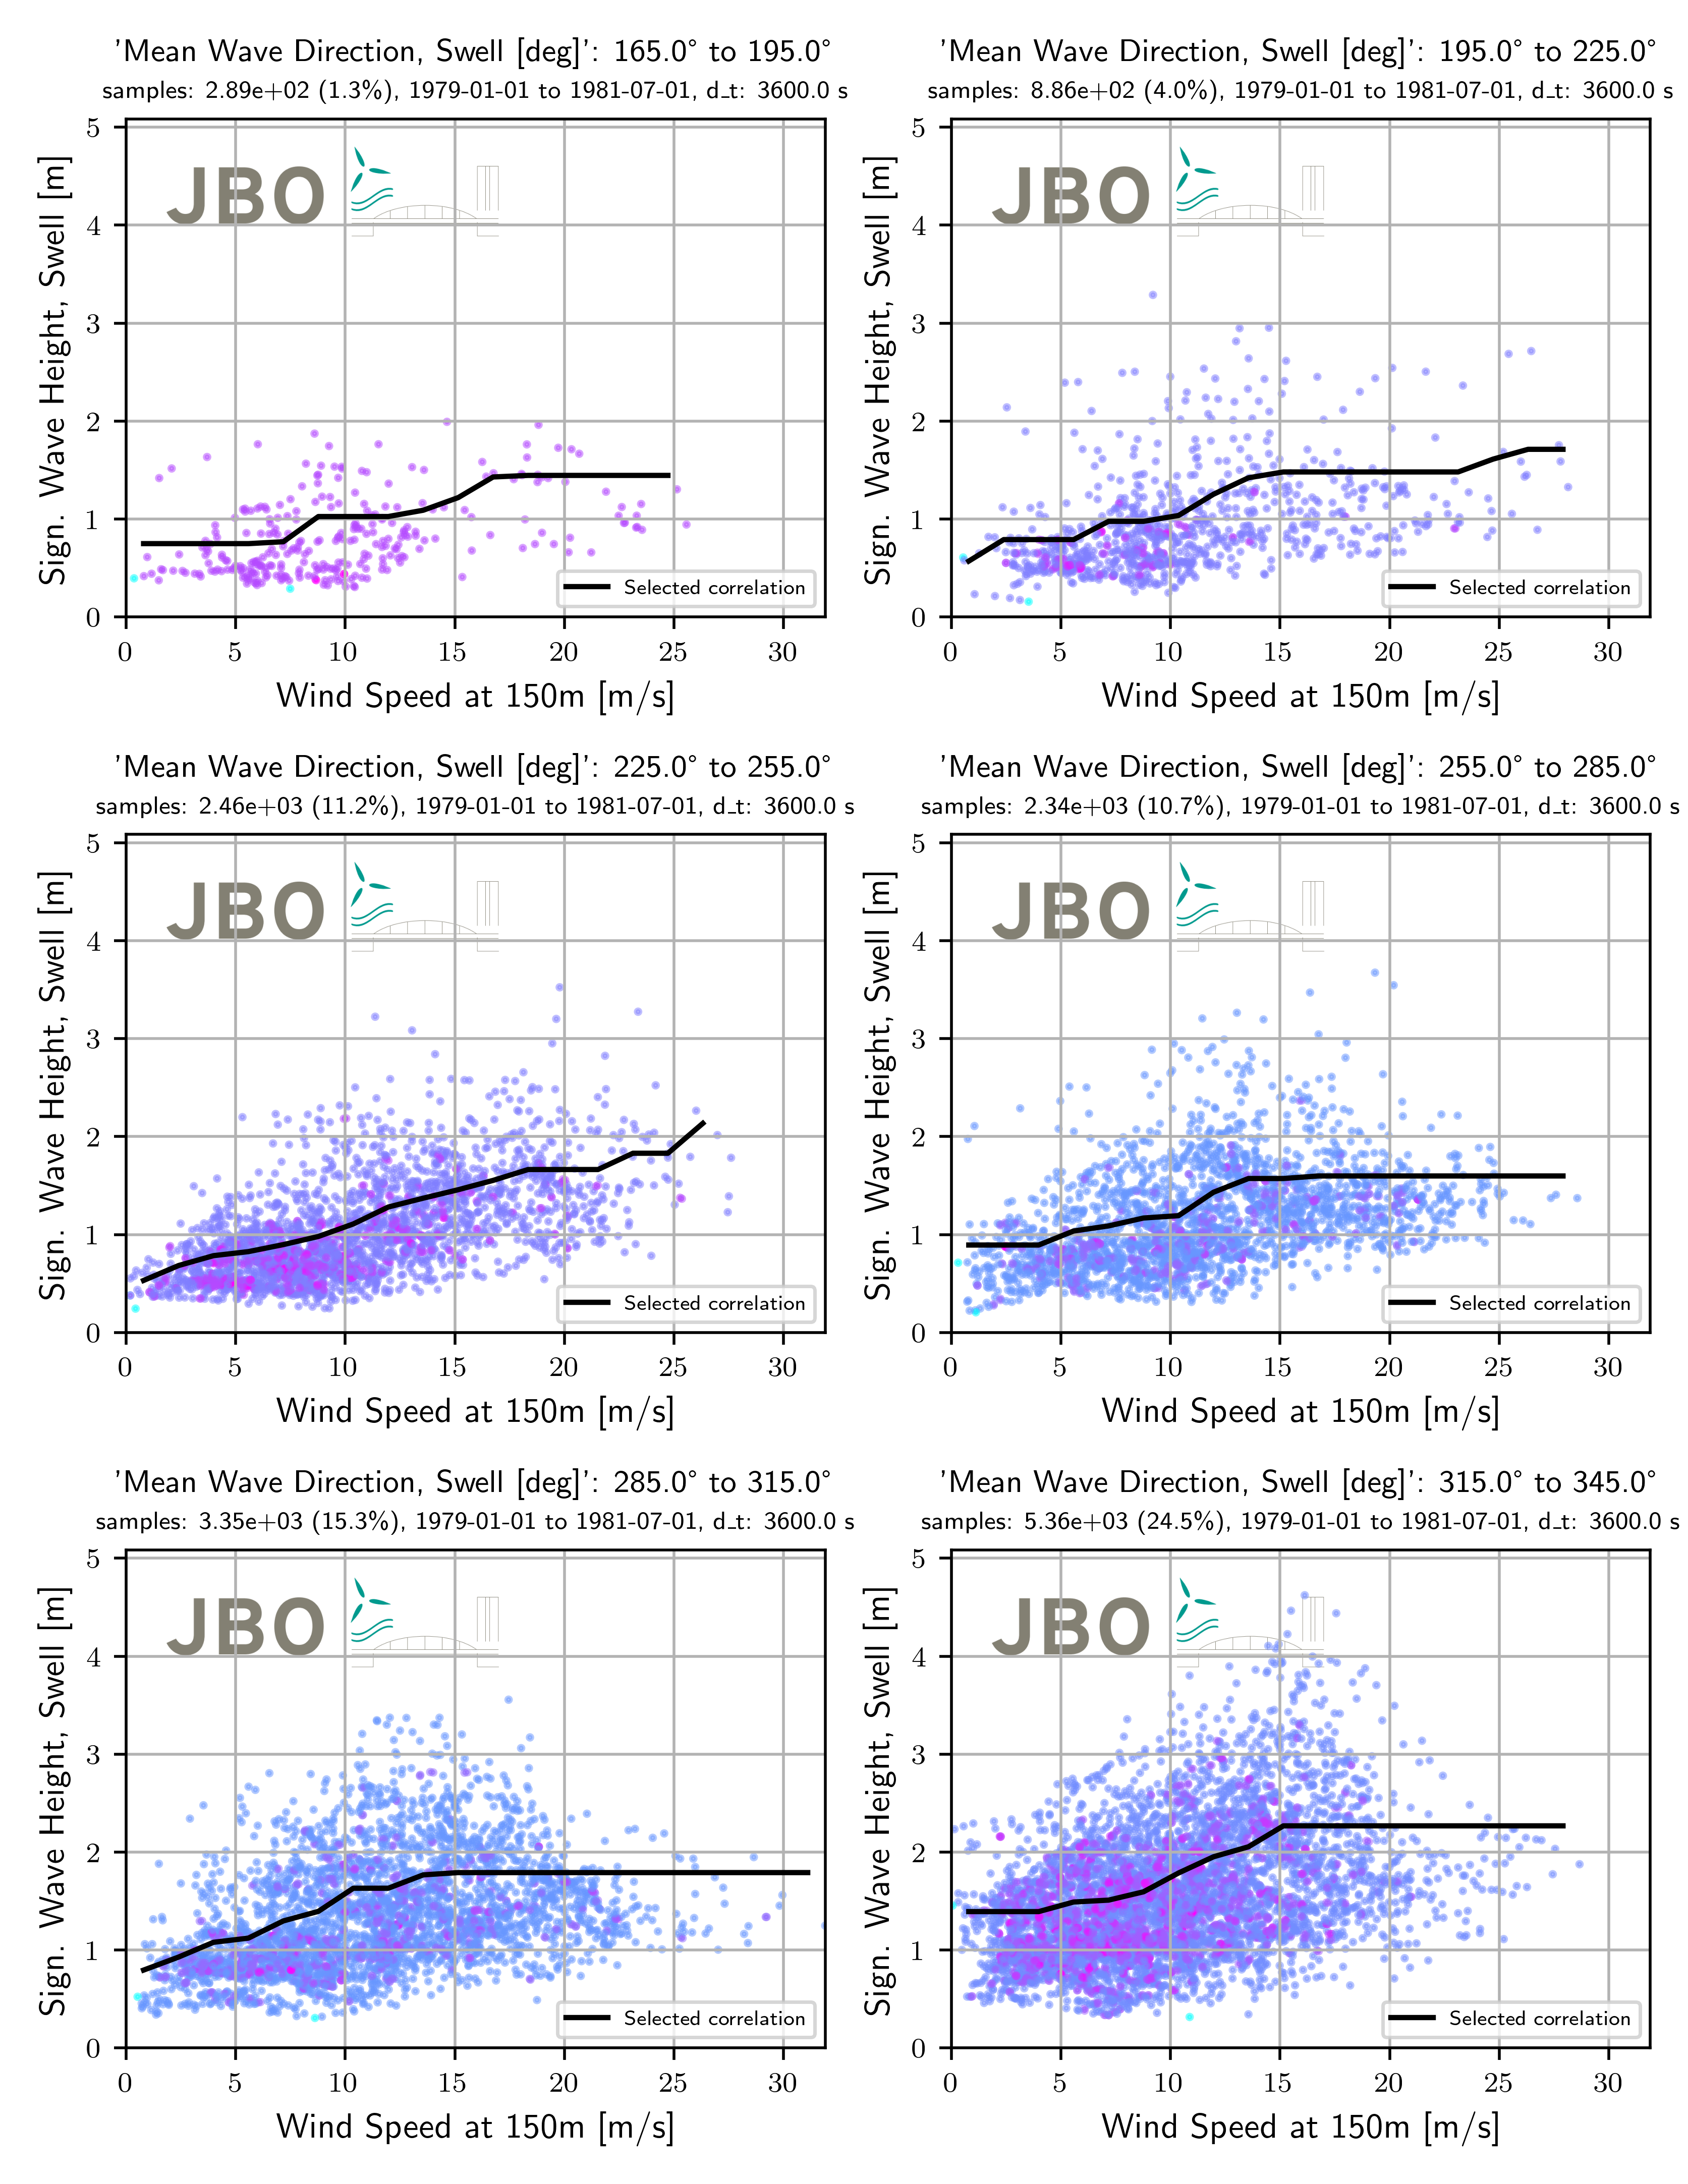
\includegraphics[width=1.0\textwidth]{C:/Users/aaron.lange/Desktop/Projekte/Hindcast_Tool/HindTool/example_output/VMHS_swell_page_2.png} 
 \caption{ VMHS-swell-page-2 } 
 \label{fig: VMHS_swell_page_2 } 
\end{figure}


\subsubsection{Peak period over wind speed }
The cross correlation of the $T_{P}$ data to the $v_{m}$ data is needed, as it forms a sea state with corresponding $H_{S}$ data in the respective $v_{m}$-bin and directional sector. A direct correlation following from a representative value and a regression curve follows no underlying physical connection. Therefore the $v_{m}\left(T_{P}\right)$ relation is derived using the determined correlations $H_{s}\left(v_{m}\right)$ and $T_{P}\left(H_{S}\right)$.

For this, the function $H_{s}\left(v_{m}\right)$ (REF, left) is inverted to $v_{m}\left(H_{S}\right)$ (middle). This is possible because the function is bijective. The goal is to substitute this relation for $H_{S}$ in the $T_{P}\left(H_{S}\right)$ function to get to the correlation of $T_{P}\left(v_{m}\right)$. As shown, the $H_{S}$-values in the horizontal axis aren't equidistant anymore as they are in the $T_{P}\left(H_{S}\right)$ relation. Therefore, new $v_{m}$-values must be interpolated to the appropriate $H_{S}$-values (middle). Now $H_{S}$ can be substituted for $v_{m}$ - and the $T_{P}\left(v_{m}\right)$ relation can be found (right).\\

\begin{figure}[H] 
 \centering 
 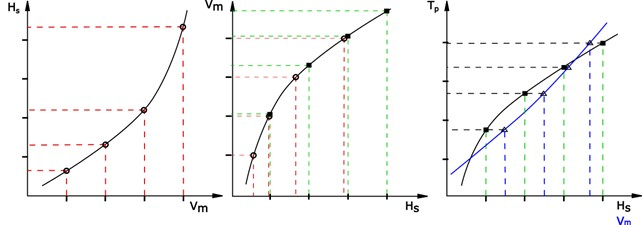
\includegraphics[width=1.0\textwidth]{C:/Users/aaron.lange/Desktop/Projekte/Hindcast_Tool/HindTool/latex_templates/VMTP_theory.jpg} 
 \caption{ Cross correlation for determining peak period over wind speed } 
 \label{fig: VMTP_theory } 
\end{figure}
\begin{figure}[H] 
 \centering 
 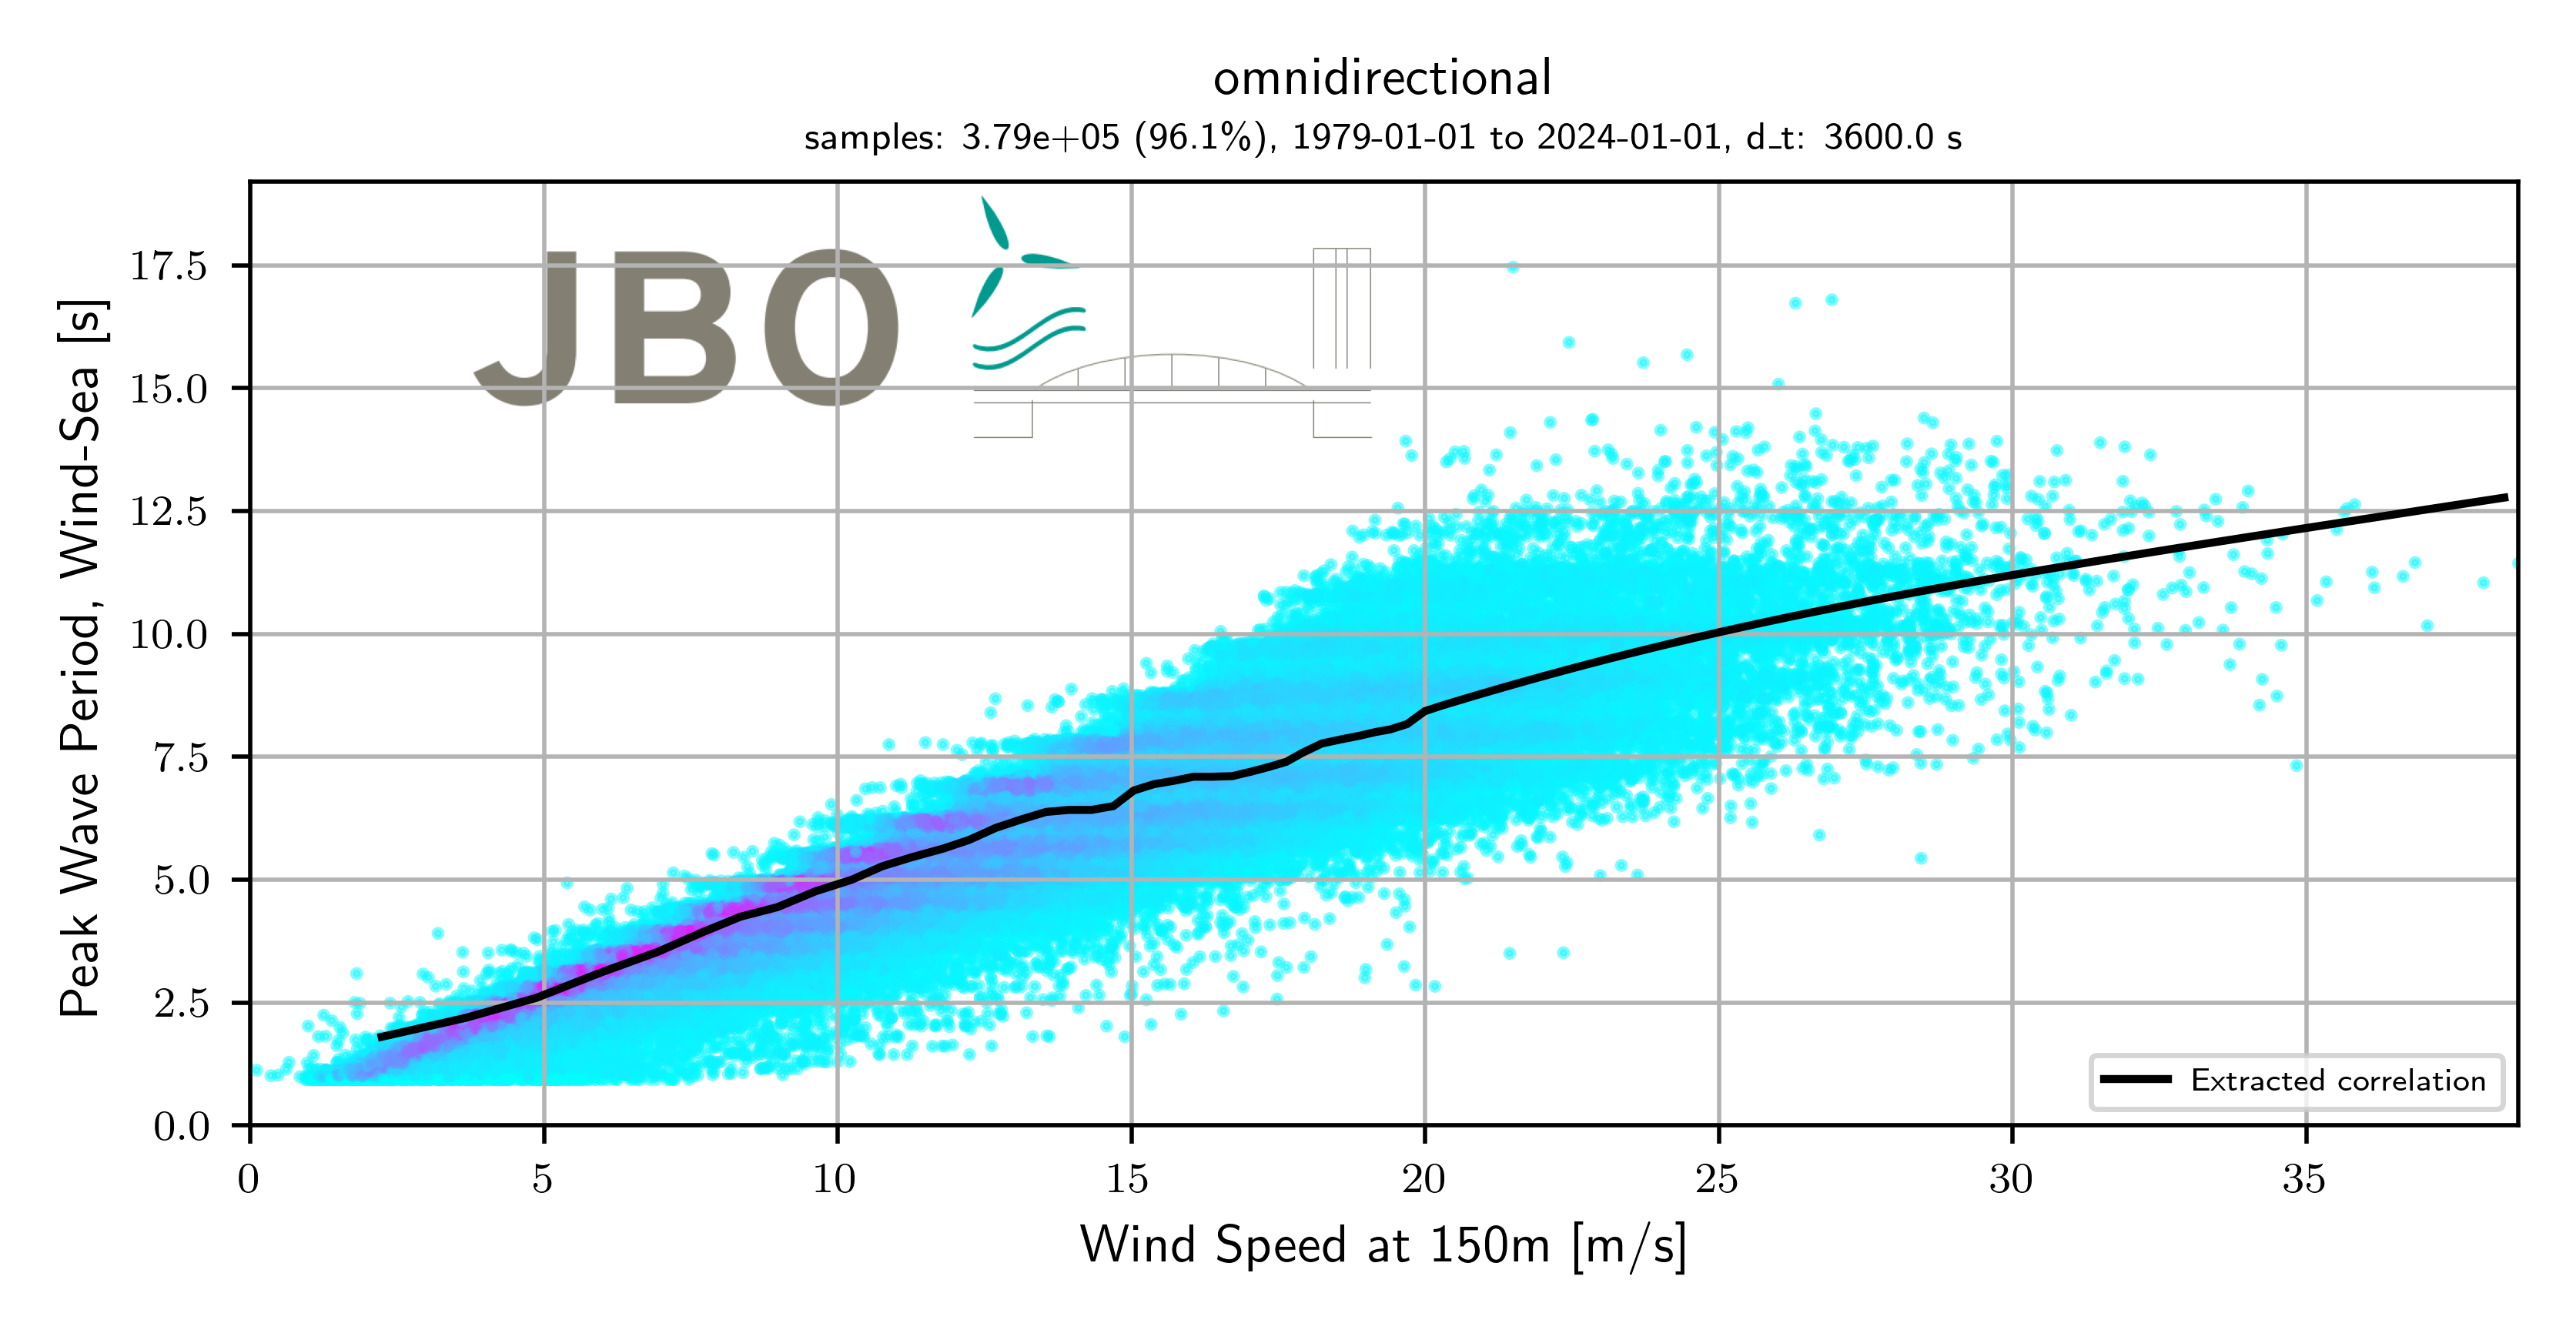
\includegraphics[width=1.0\textwidth]{C:/Users/aaron.lange/Desktop/Projekte/Hindcast_Tool/HindTool/example_output/VMTP_wind_page_3.png} 
 \caption{ VMTP-wind-page-3 } 
 \label{fig: VMTP_wind_page_3 } 
\end{figure}

\subsubsection{Summary tables of normal sea state conditions}
For the final condensation of the sea state-parameters the $H_s$ and $T_p$ values are determined using the $H_s(V_s)$ and $T_p(V_m)$ correlations. Therefore, the small-gridded functions are used to interpolate the data on the desired v_m- grid. The values are only calculated in the $v_m$ - range with data given. Bins inside the evaluated limits with zero occurrence probabilities are greyed out. The results are displayed in the tables (REF).

\begin{figure}[H] 
 \centering 
 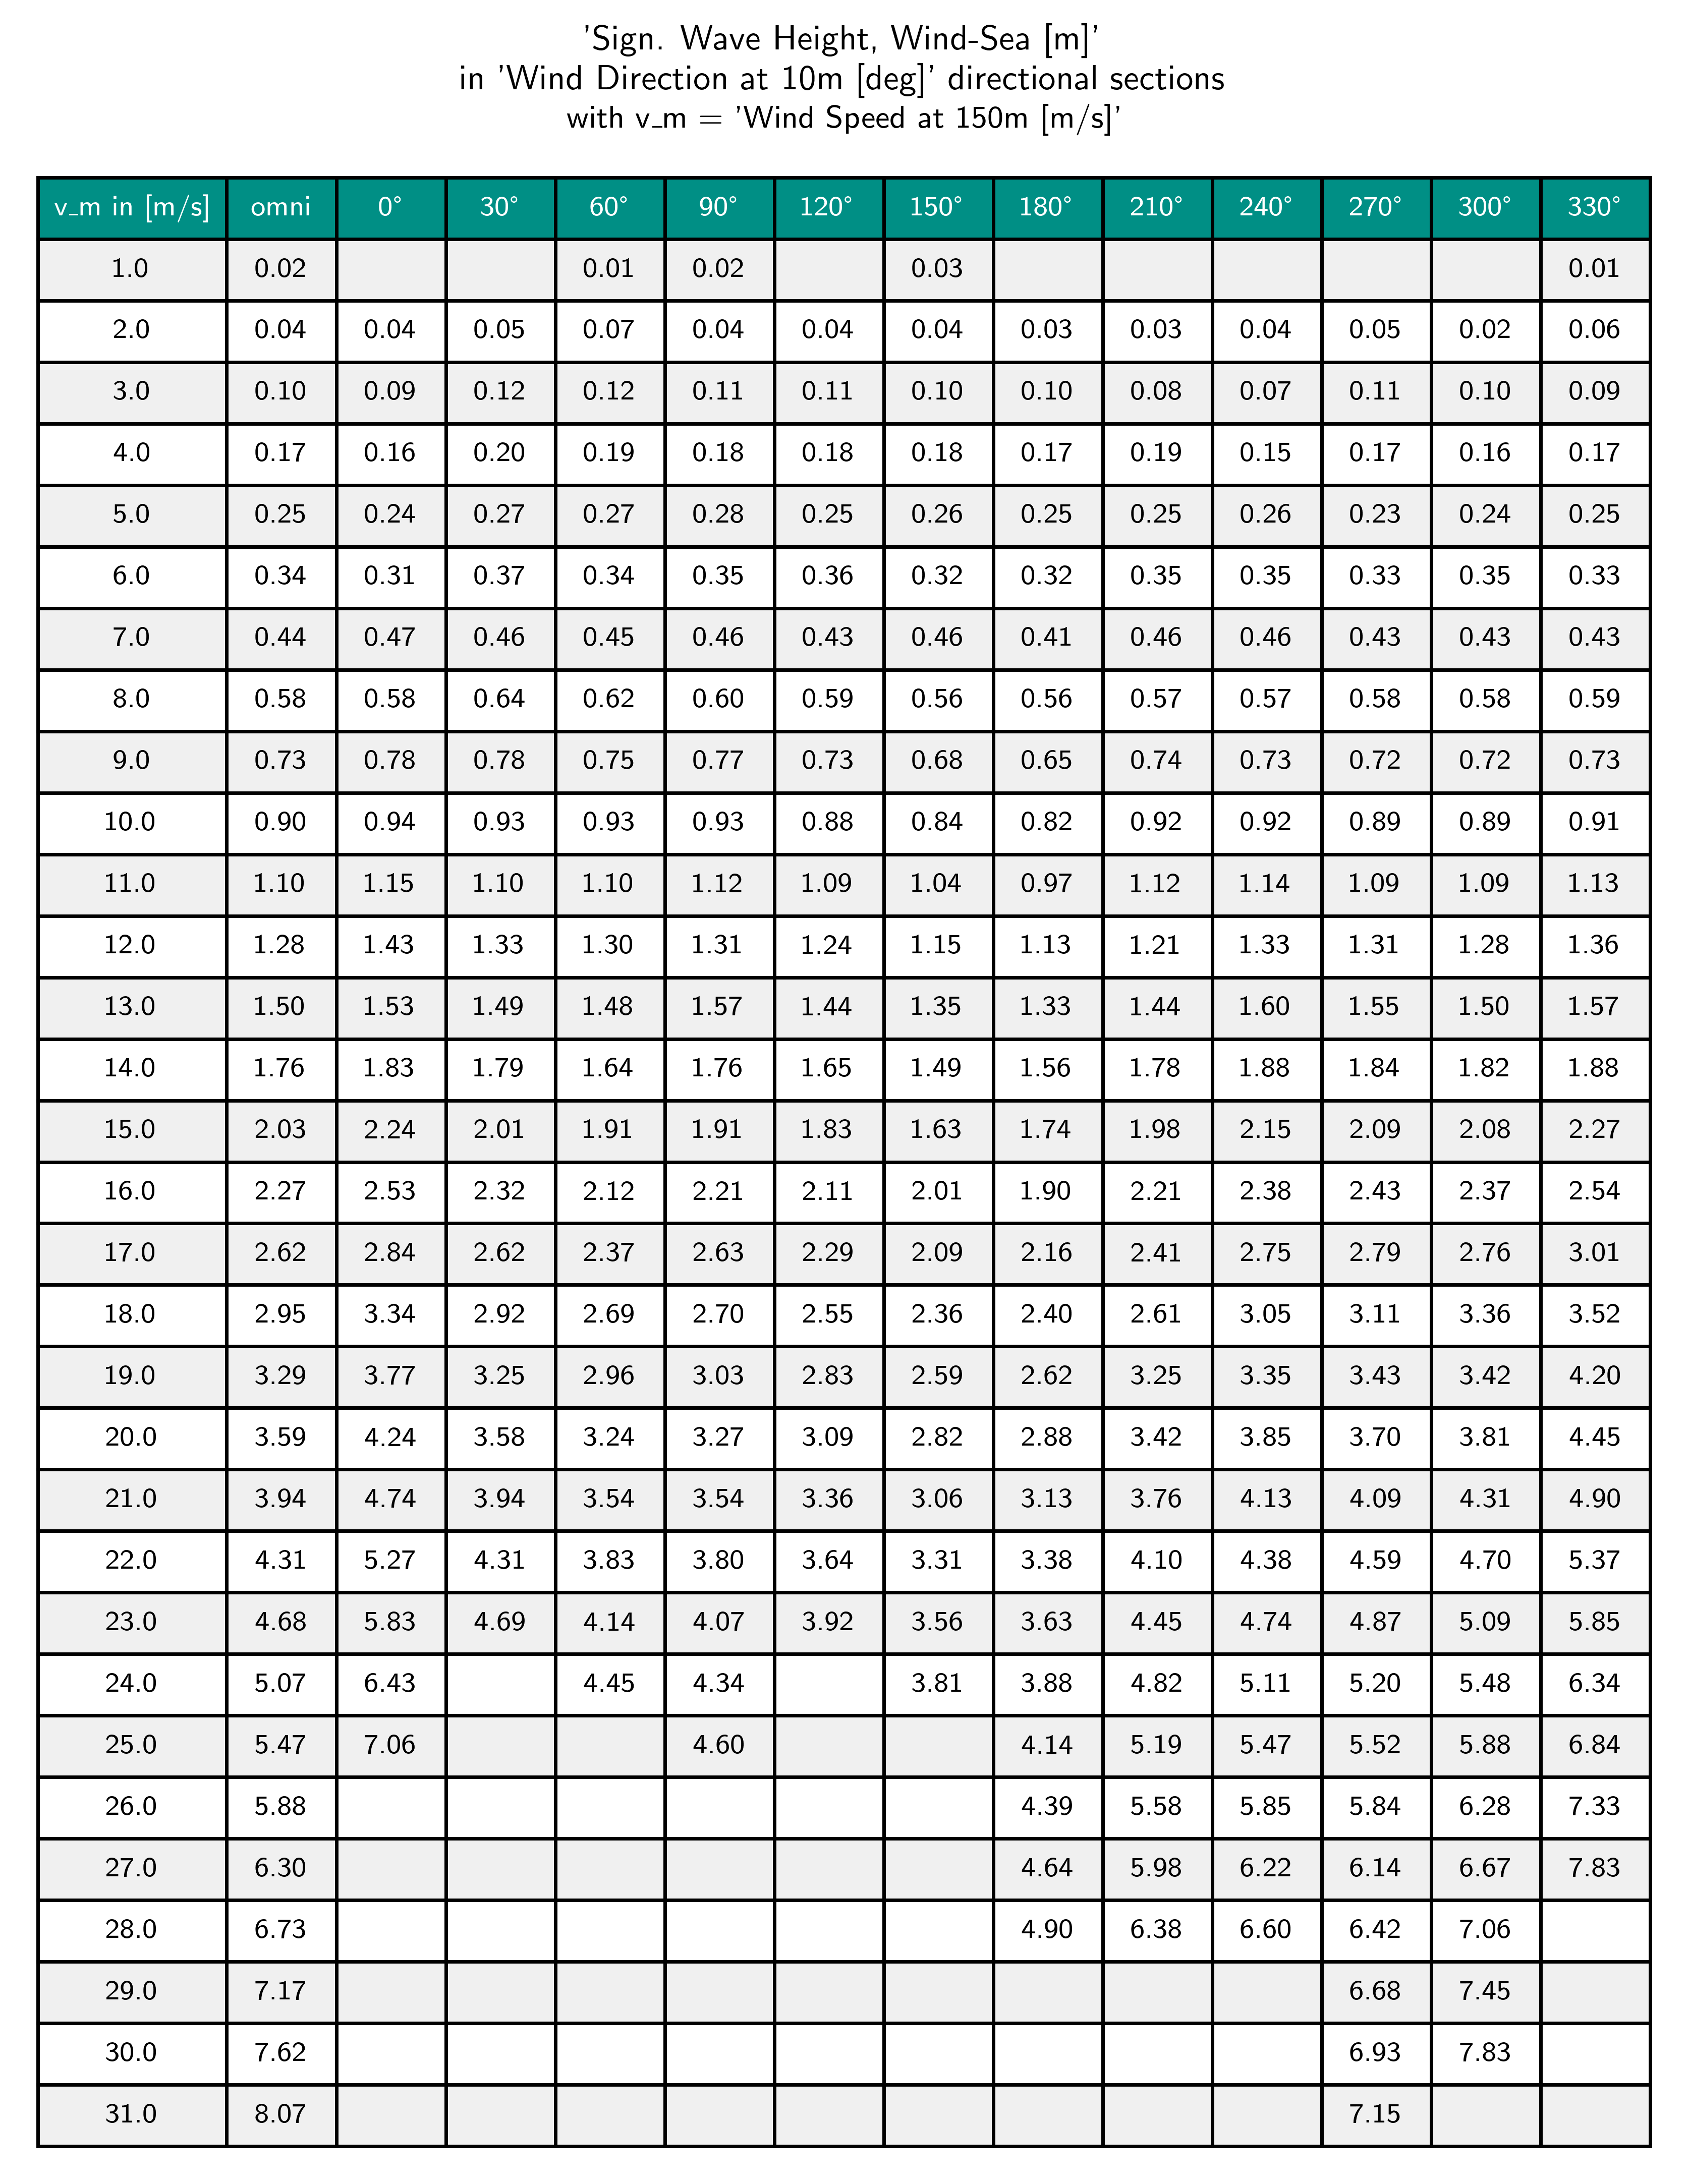
\includegraphics[width=1.0\textwidth ]{C:/Users/aaron.lange/Desktop/Projekte/Hindcast_Tool/HindTool/example_output/table_vmhs_wind_page_1.png} 
 \captionsetup{type=table} 
\caption{ table-vmhs-wind-page-1 } 
 \label{tab: table_vmhs_wind_page_1 } 
\end{figure}
\begin{figure}[H] 
 \centering 
 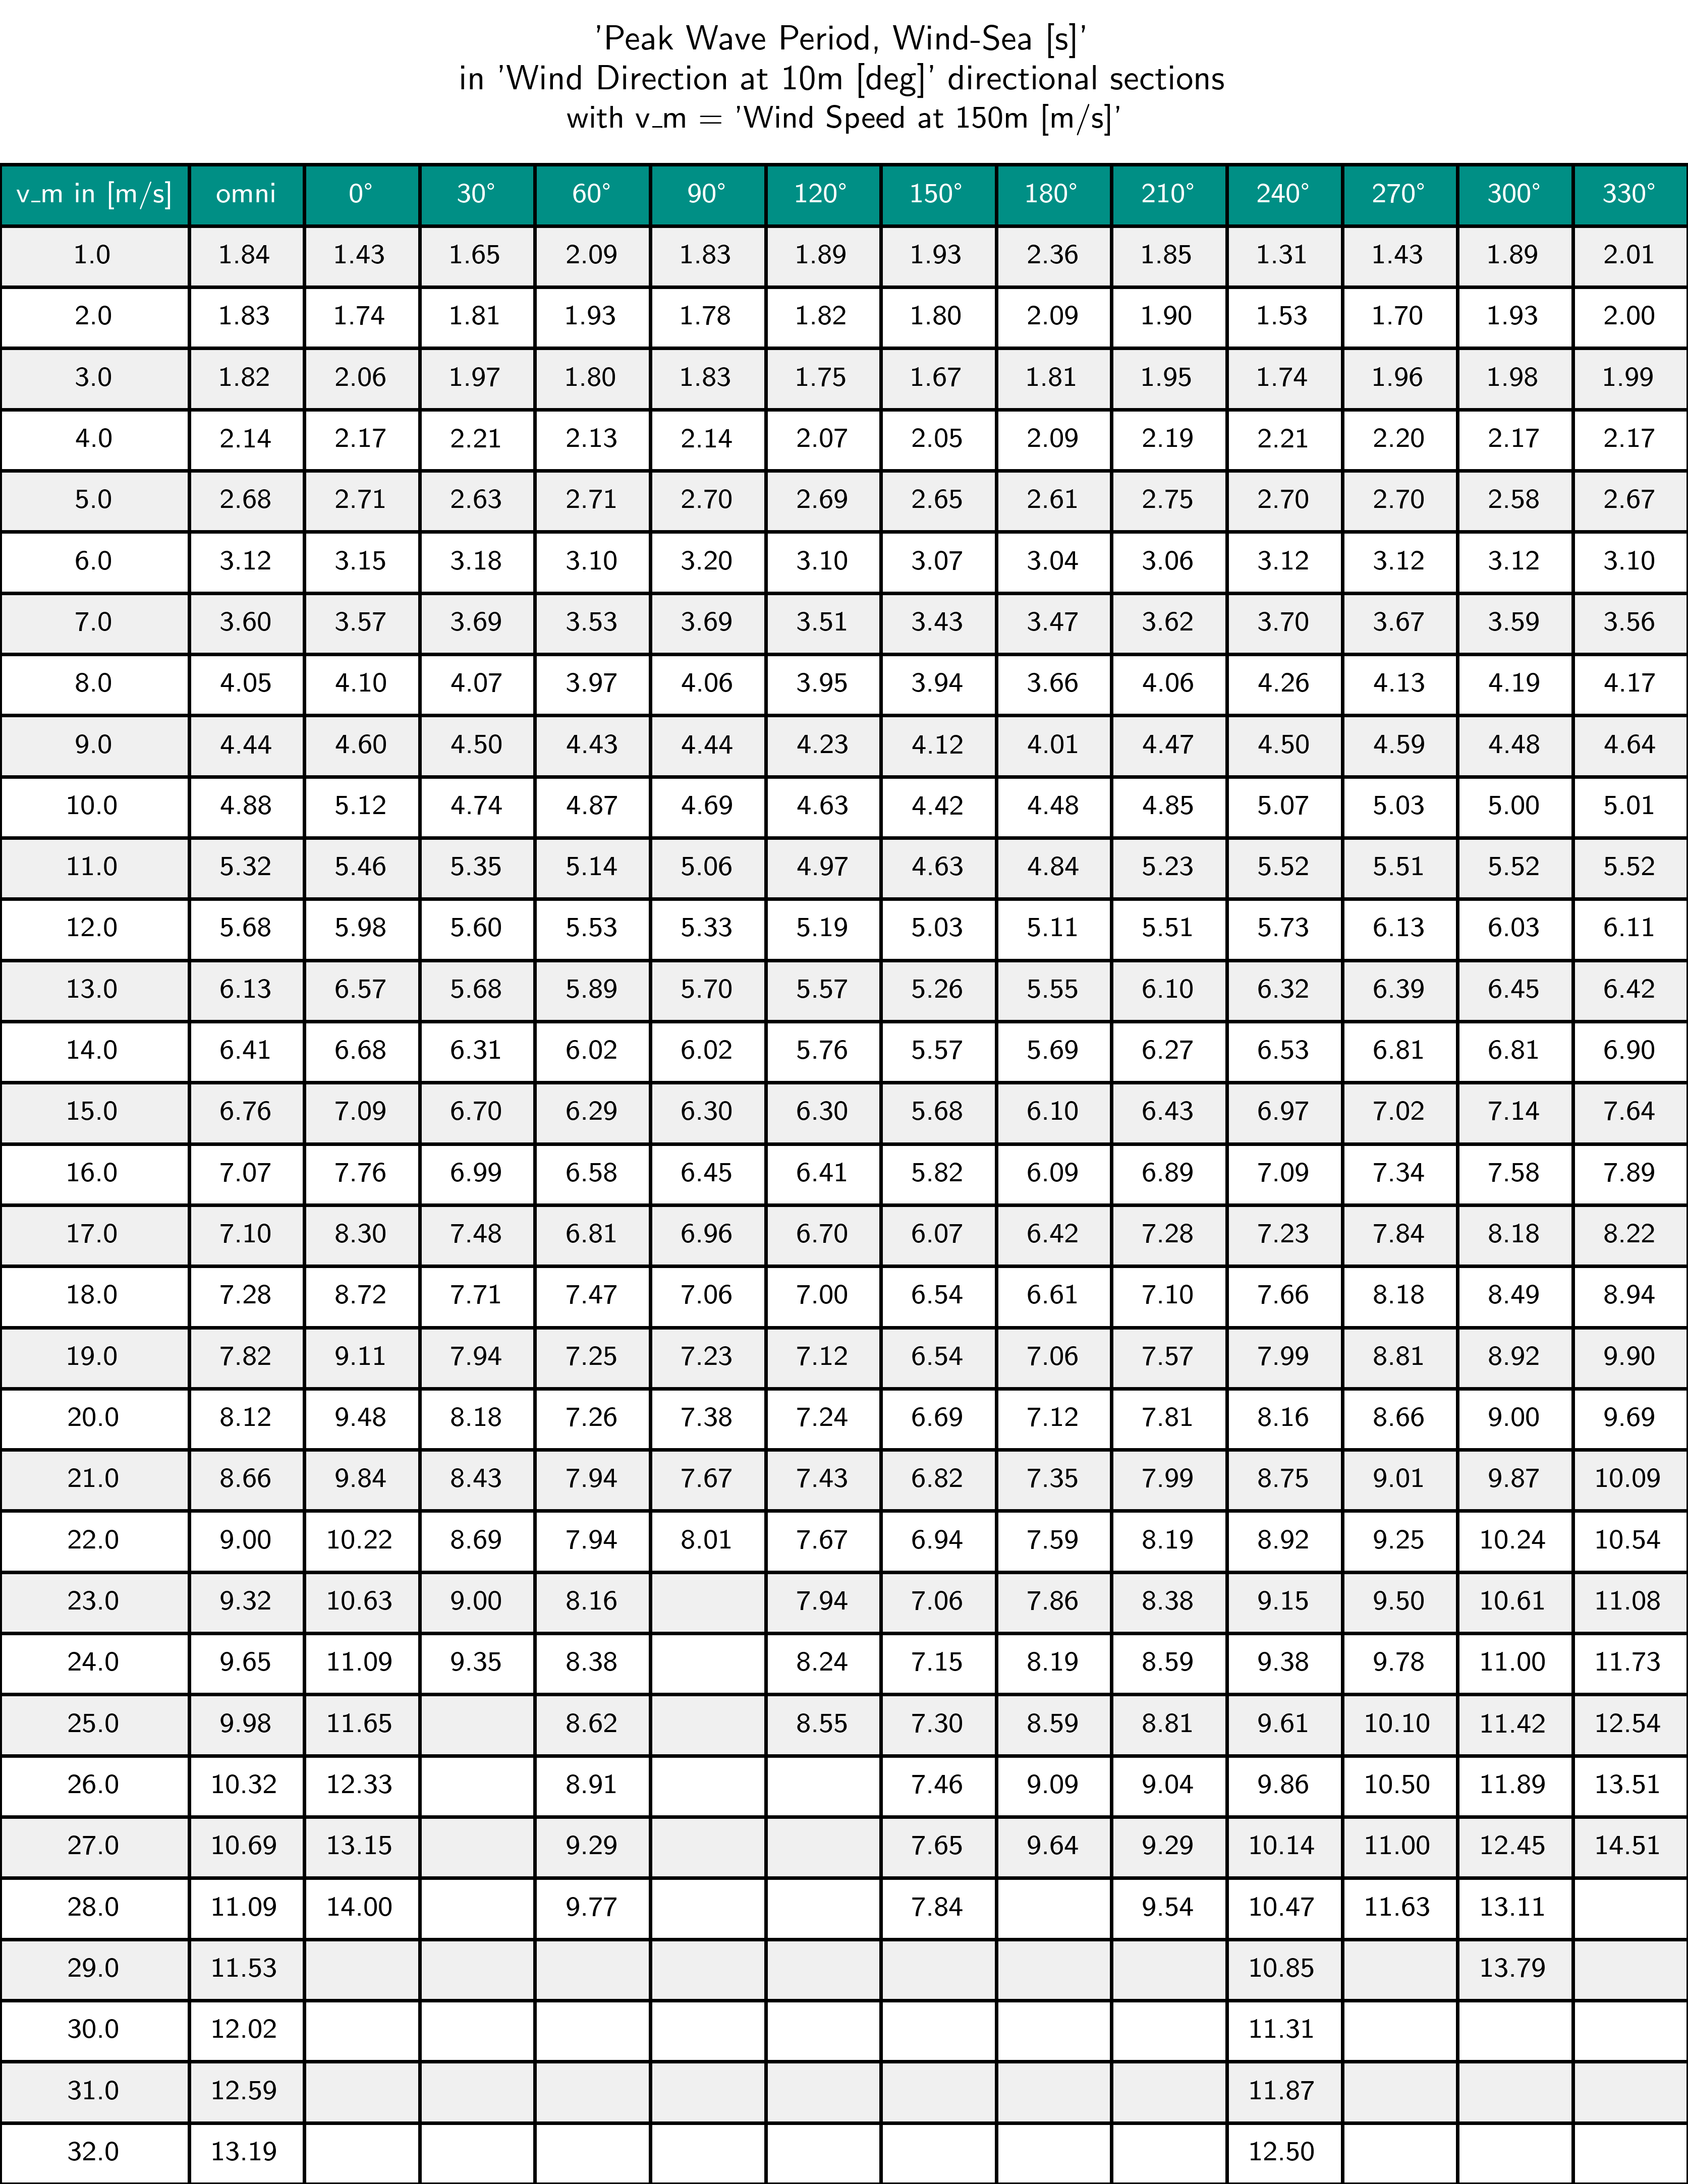
\includegraphics[width=1.0\textwidth ]{C:/Users/aaron.lange/Desktop/Projekte/Hindcast_Tool/HindTool/example_output/table_vmtp_wind_page_1.png} 
 \captionsetup{type=table} 
\caption{ table-vmtp-wind-page-1 } 
 \label{tab: table_vmtp_wind_page_1 } 
\end{figure}
\begin{figure}[H] 
 \centering 
 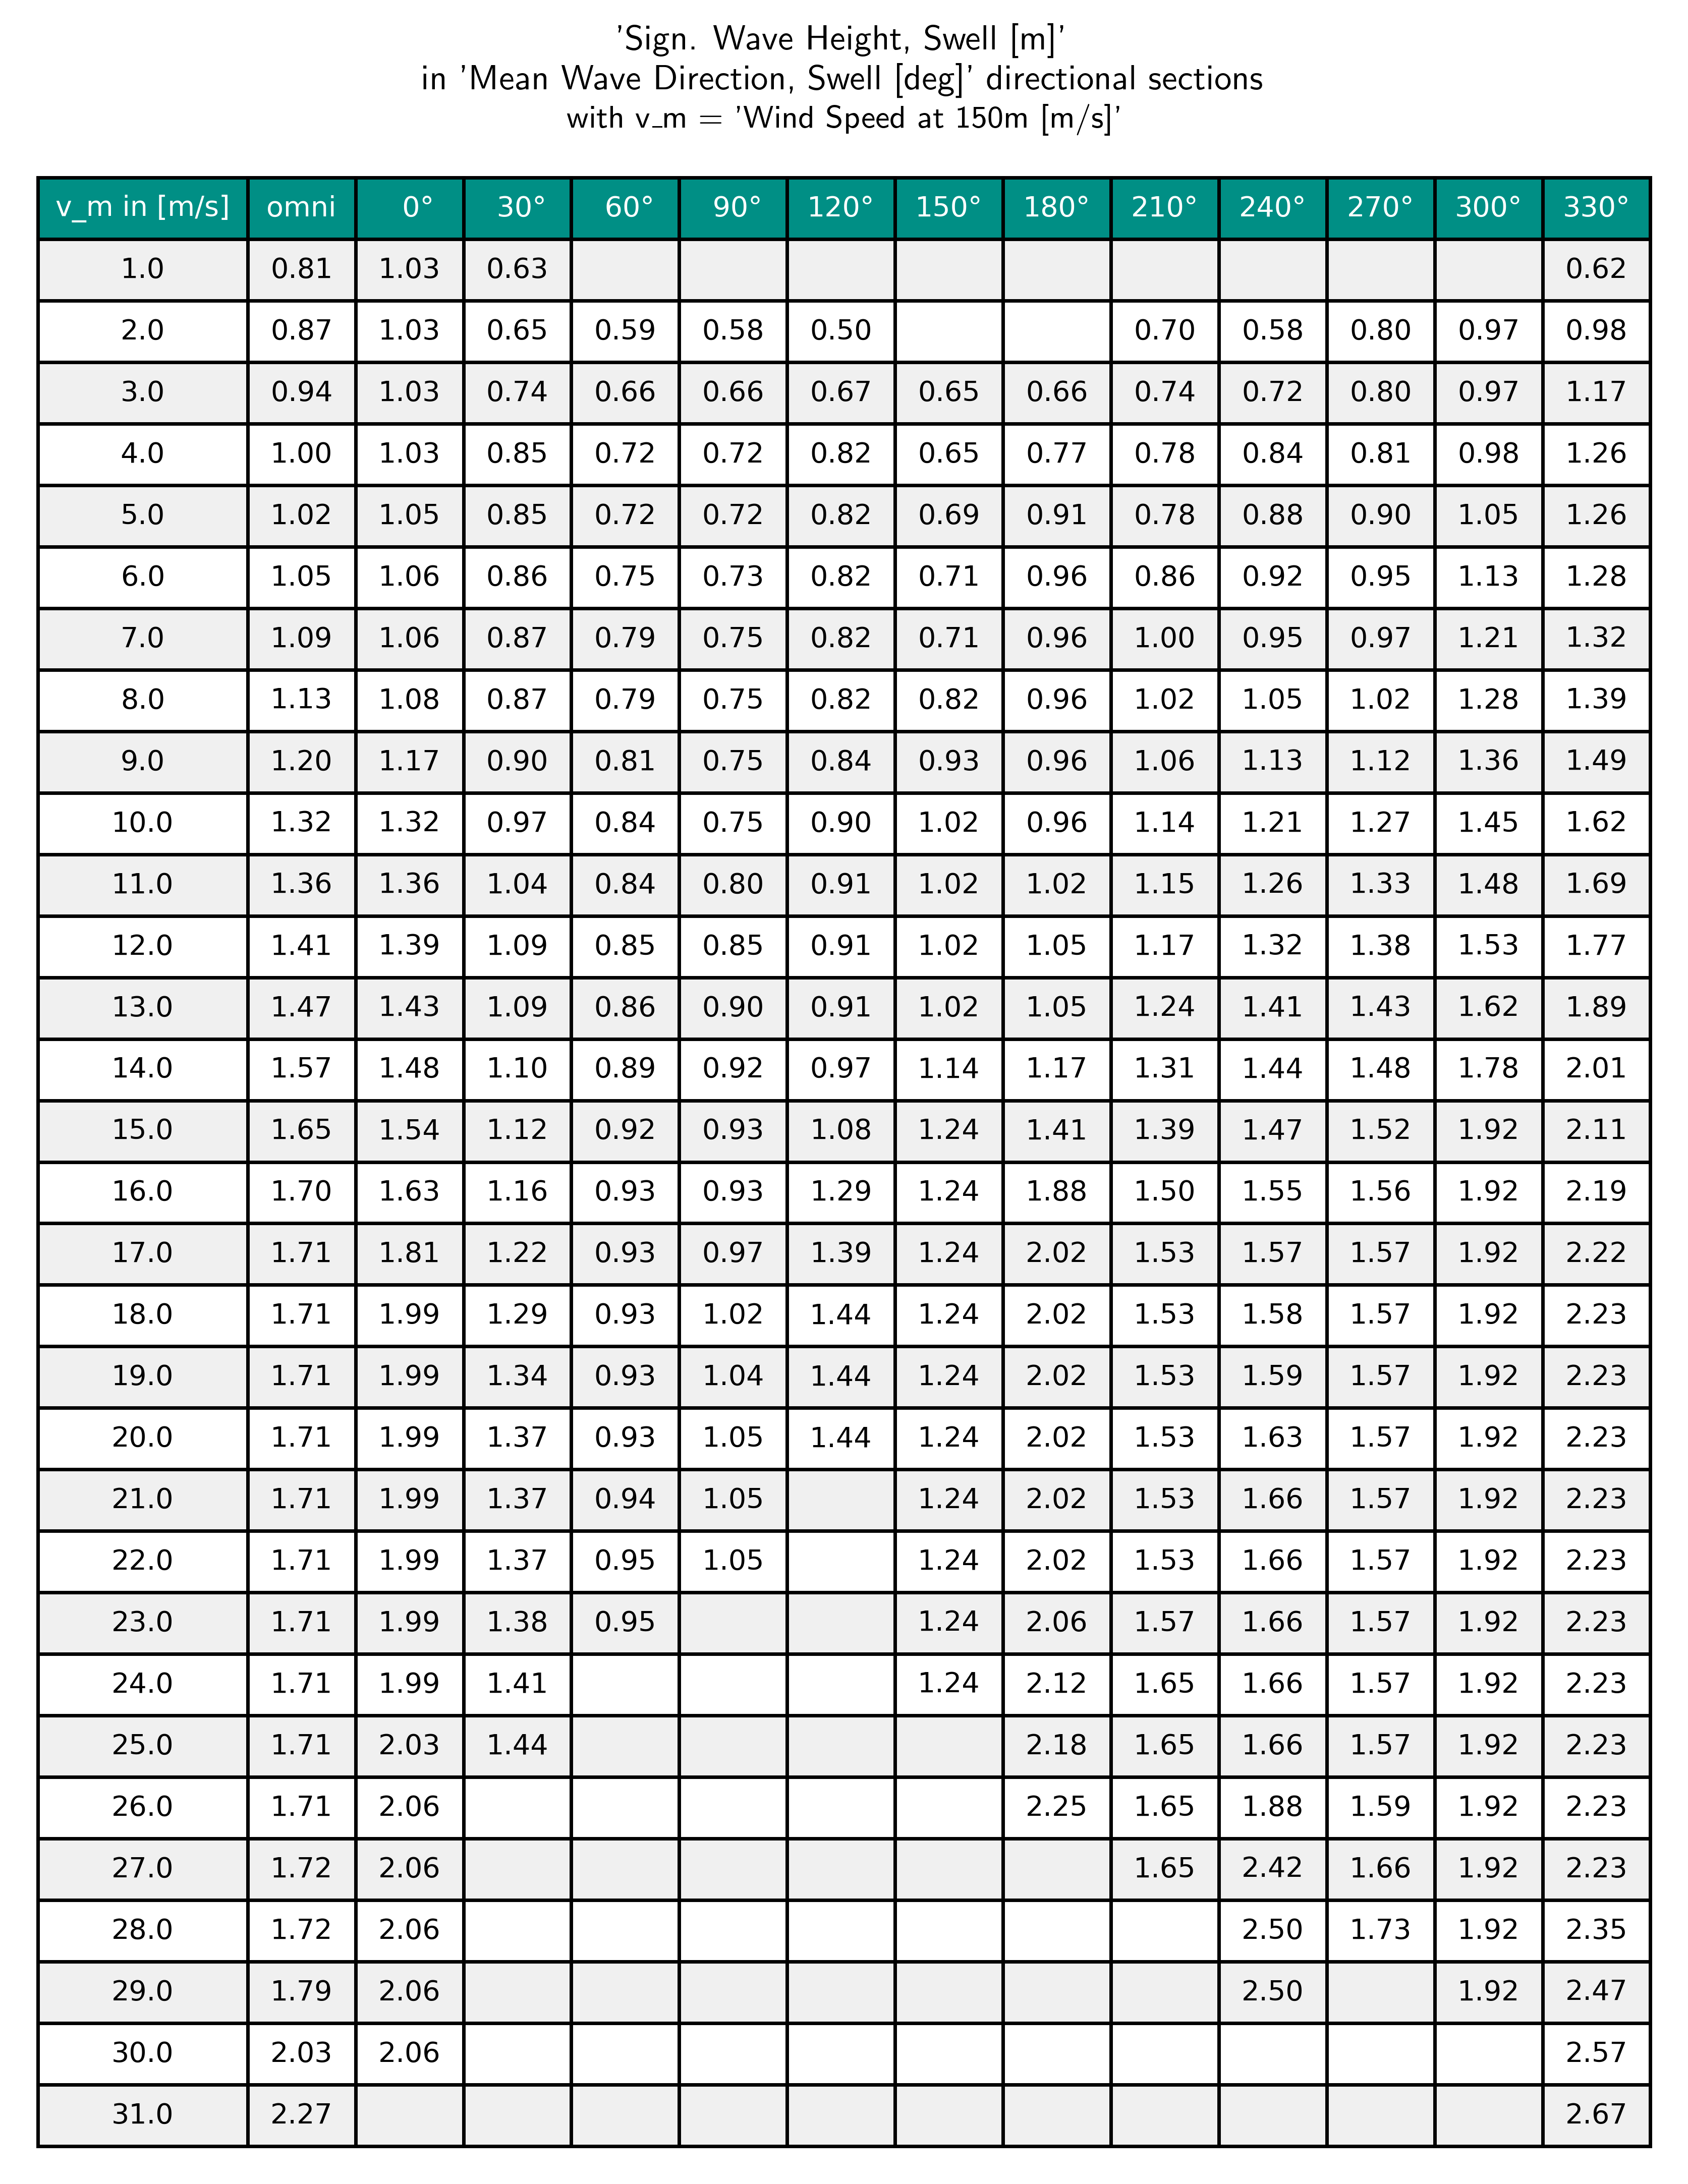
\includegraphics[width=1.0\textwidth ]{C:/Users/aaron.lange/Desktop/Projekte/Hindcast_Tool/HindTool/example_output/table_vmhs_swell_page_1.png} 
 \captionsetup{type=table} 
\caption{ table-vmhs-swell-page-1 } 
 \label{tab: table_vmhs_swell_page_1 } 
\end{figure}
\begin{figure}[H] 
 \centering 
 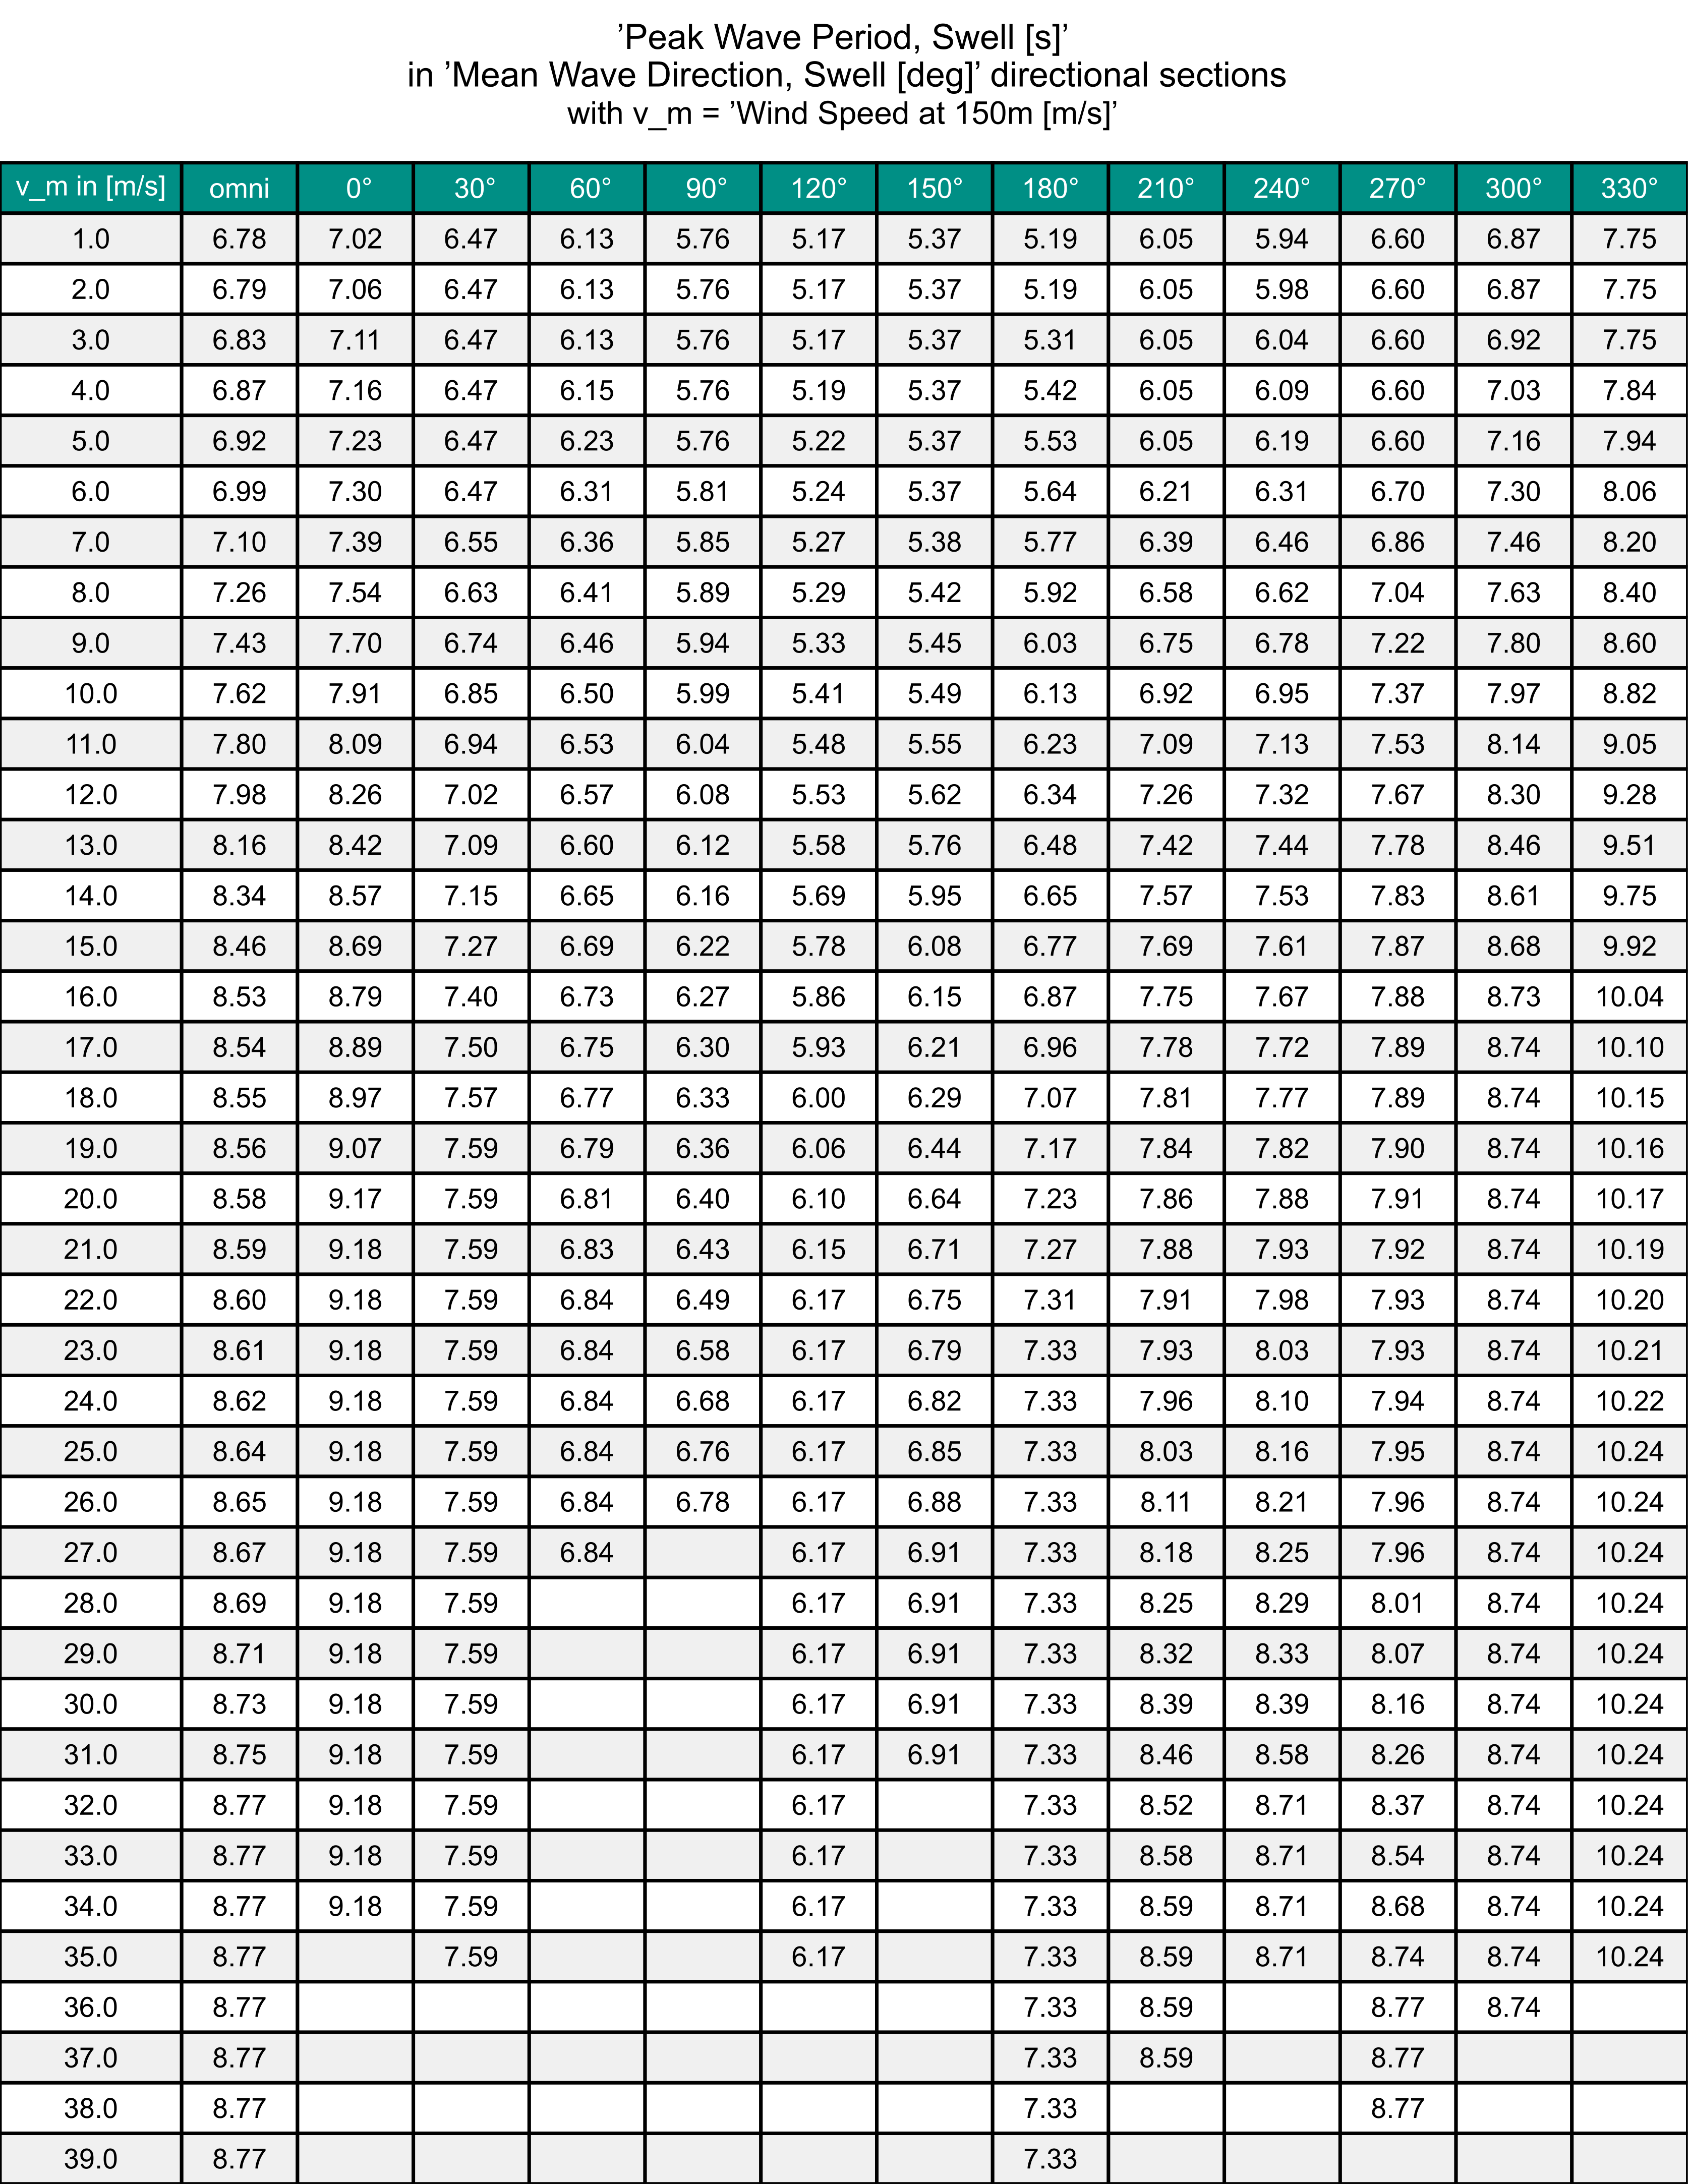
\includegraphics[width=1.0\textwidth ]{C:/Users/aaron.lange/Desktop/Projekte/Hindcast_Tool/HindTool/example_output/table_vmtp_swell_page_1.png} 
 \captionsetup{type=table} 
\caption{ table-vmtp-swell-page-1 } 
 \label{tab: table_vmtp_swell_page_1 } 
\end{figure}

\subsection{Proof of condensation method}
The proof of the condensation method for normal sea state parameter is provided in this section in detail. A reference structural FE model of the intended WTG and foundation configuration has been set up for this purpose. Using a frequency domain approach, damage equivalent loads of the bending moment at decisive elevations are calculated for each individual sea state sample in the data set.
\\
Damage equivalent loads are applied to equate the fatigue damage represented by rainflow cycle counted data to that caused by a single stress range repeating at a single frequency. The method is based on the Miner's rule. The damage equivalent load is given by the following formula:

$$
L_{N}(m)=\sqrt[m]{\frac{\sum_{i=1}^{k} L_{i}^{m} n_{i}}{N}}
$$

where:
\quad $ L_{N} $ \quad is the equivalent stress for $N$ cycles in the specified design life\\
\quad $ L_{i} $ \quad is the stress range bin $i$\\
\quad $ n_{i} $ \quad is the number of rain flow cycles at stress range bin $i$\\
\quad $ k $ \quad  is the number of bins\\
\quad $ m $ \quad  is the negative inverse of the slope on the material's Woehler curve (m is also referred to as the S-N curve slope) \\
\quad $ N $ \quad  is the reference number of cycle repetitions (1E7 in this case) \\

The stress, $L_{i}$ depends upon the geometry of the structure. It is assumed that stress is proportional to load, therefore it is acceptable to use load instead of stress in the above equation.
\\
An overview of the load analysis results for an exemplary bending moment in frequency domain for the reference structure ( $1^{\text {st }} \mathrm{EF}=f_{0}$ ) is provided below.\\

\begin{figure}[H] 
 \centering 
 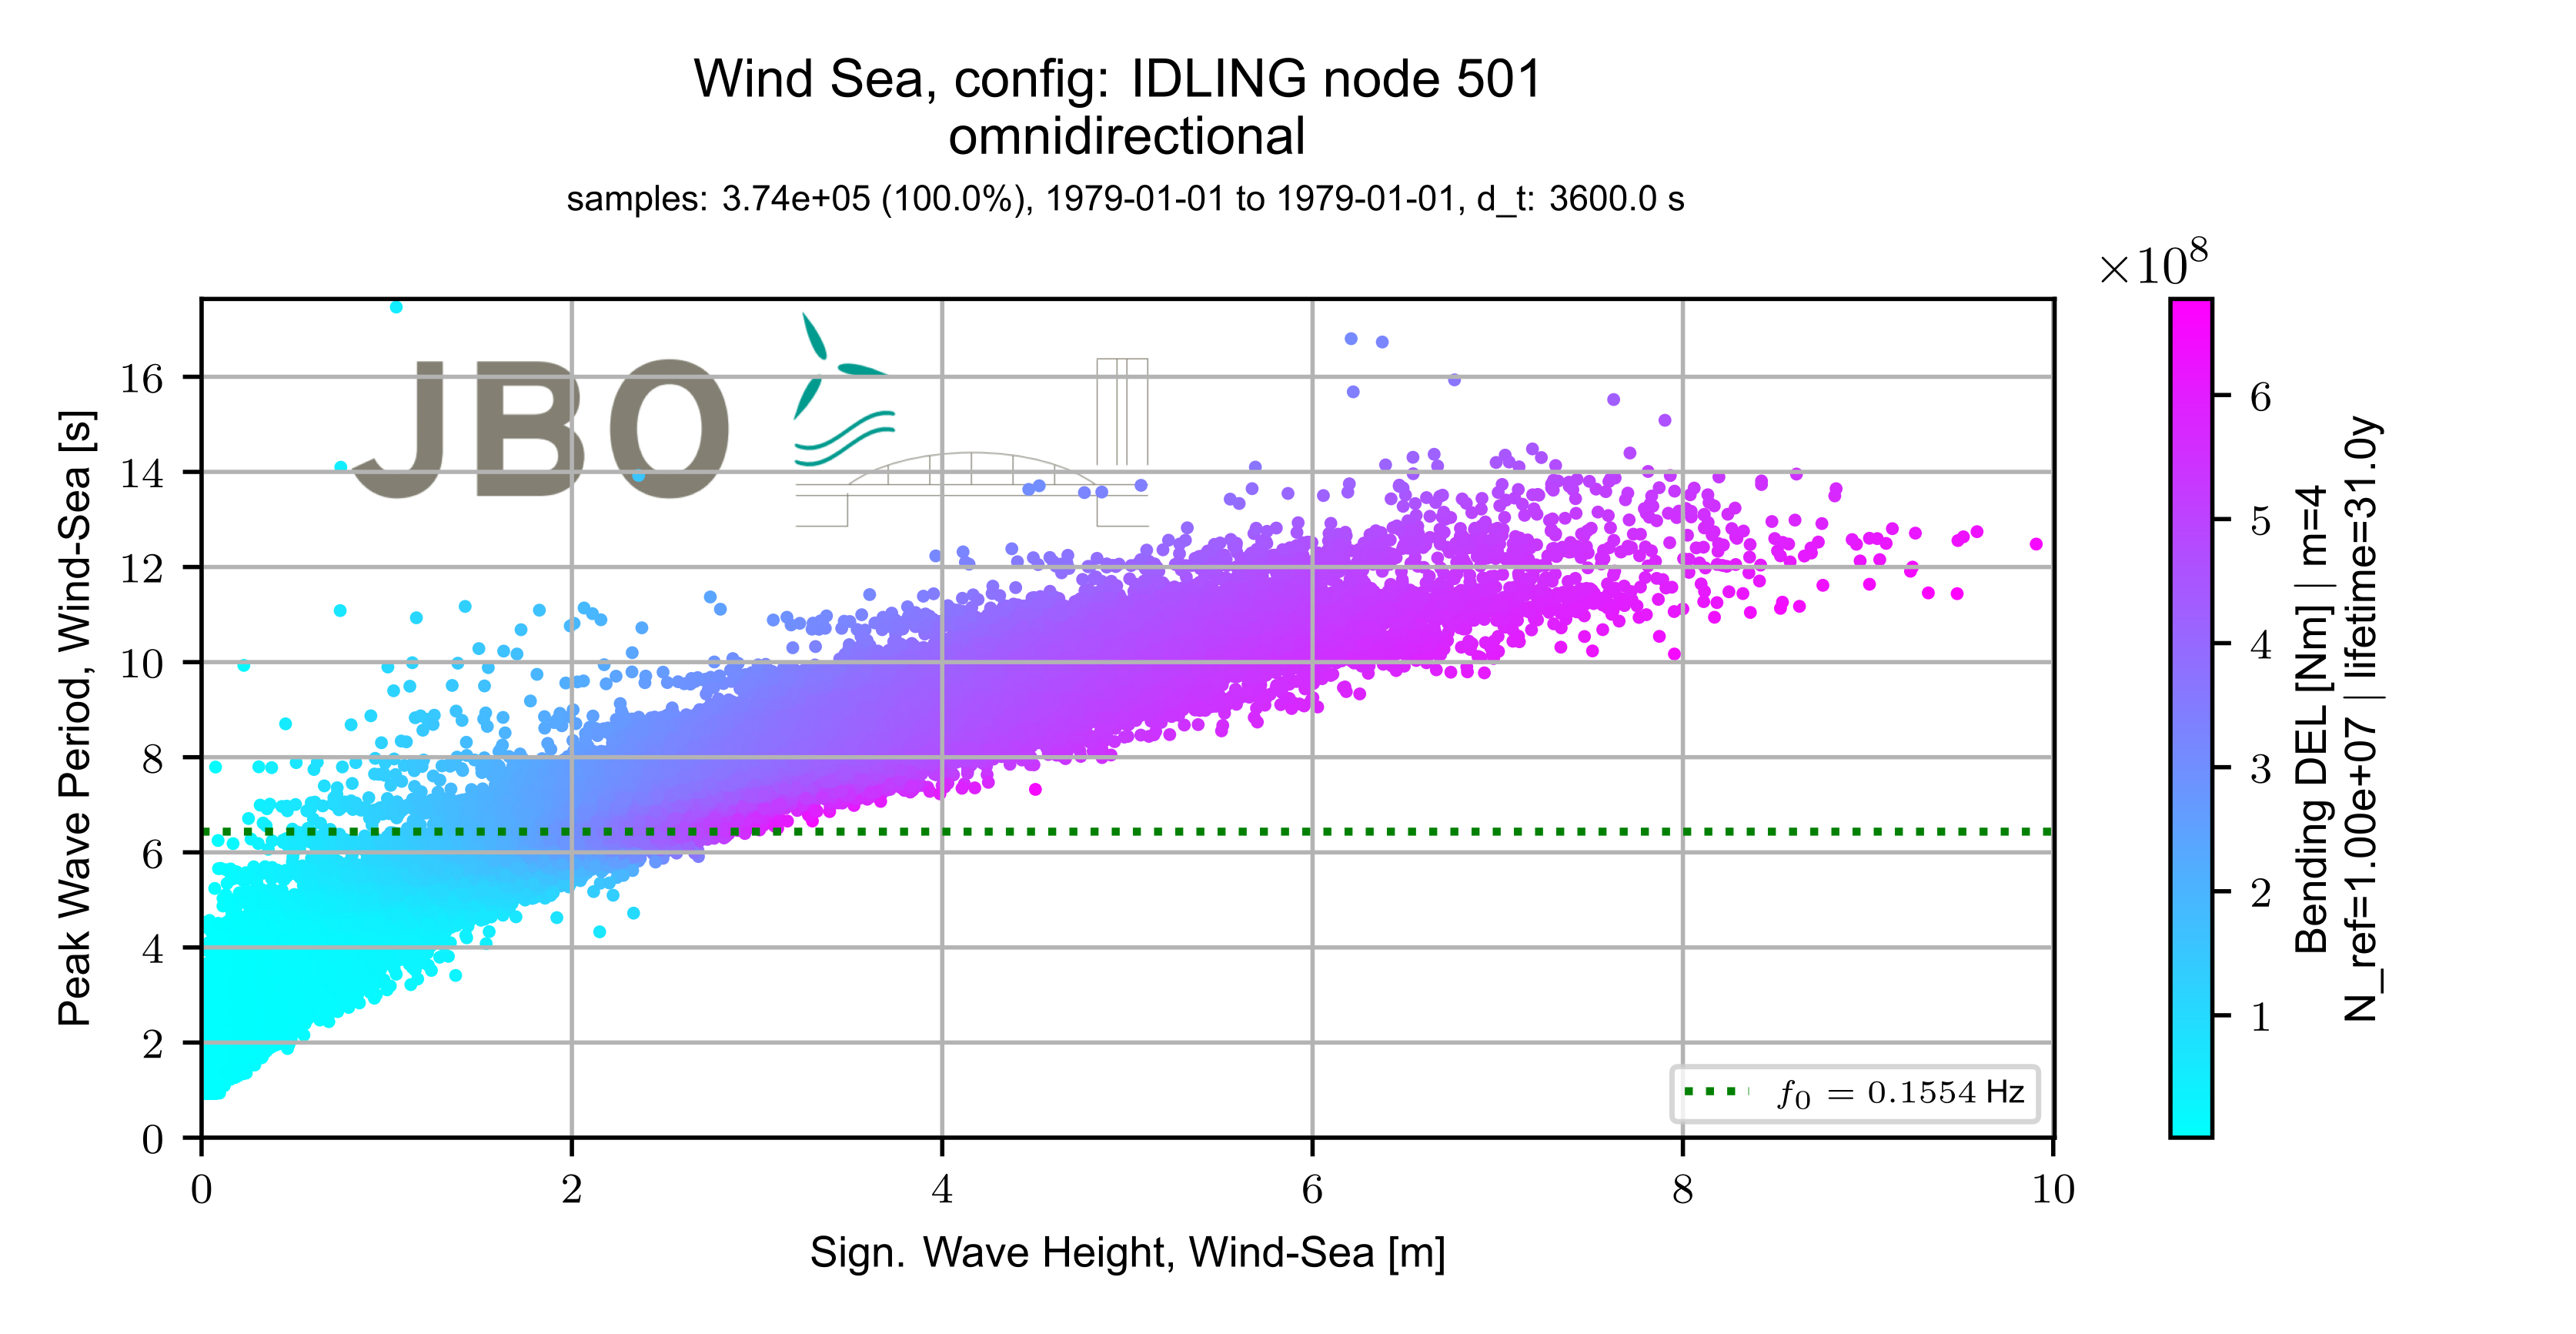
\includegraphics[width=1.0\textwidth]{C:/Users/aaron.lange/Desktop/Projekte/Hindcast_Tool/HindTool/example_output/Valid_scatter_wind_page_3.png} 
 \caption{ Valid-scatter-wind-page-3 } 
 \label{fig: Valid_scatter_wind_page_3 } 
\end{figure}
\begin{figure}[H] 
 \centering 
 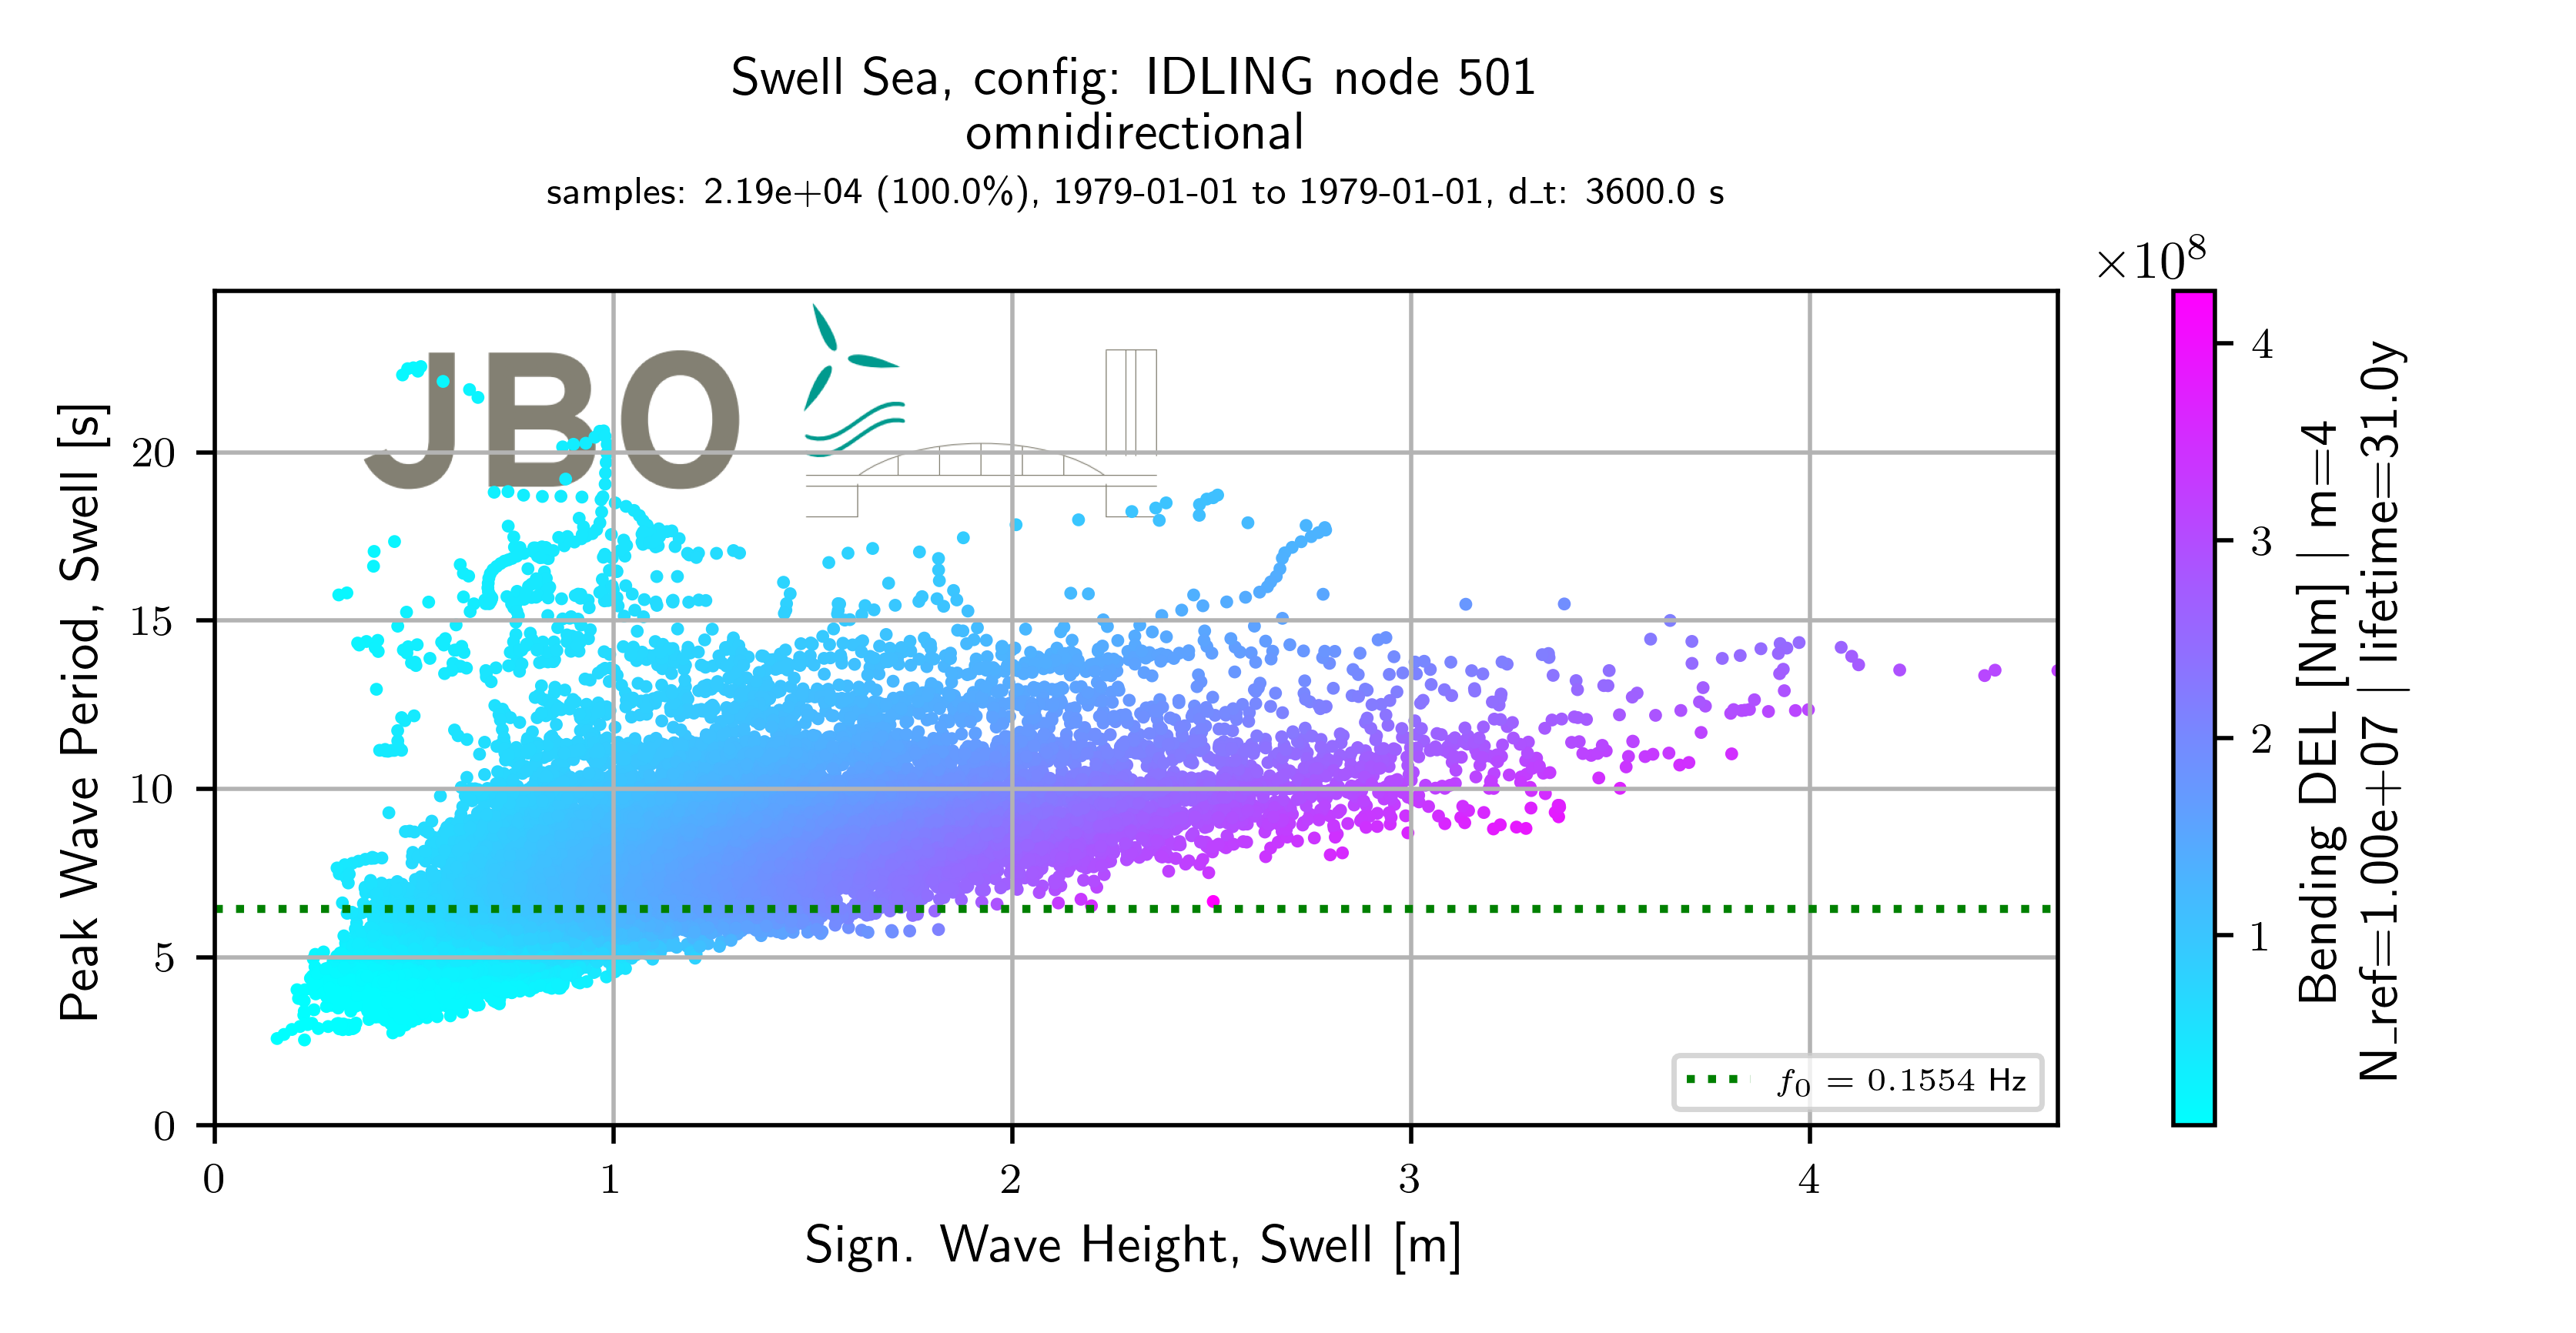
\includegraphics[width=1.0\textwidth]{C:/Users/aaron.lange/Desktop/Projekte/Hindcast_Tool/HindTool/example_output/Valid_scatter_swell_page_3.png} 
 \caption{ Valid-scatter-swell-page-3 } 
 \label{fig: Valid_scatter_swell_page_3 } 
\end{figure}


In the validation, DELs for idling conditions (very low aerodynamic damping contribution) and production conditions (incl. significant aerodynamic damping contribution) are determined for the condensed sea state data sets and compared against the full scatter data sets. This is performed for omnidirectional and directional sets, based on the wind or swell direction. Occurrence probabilities are evaluated from the associated wind speed sensor. Damping from soil, material, hydro and radiation as well as the tower damper are included in the analysis.
\\
Figure 4-10Figure 4-11 and Figure 4-11Figure 4-12 below show:
\begin{itemize}
	\item The total condensed DEL vs. the full scatter (hindcast) DEL (text box top right)
	\item Wind speed dependent comparison of condensed and full scatter (hindcast) DEL
	\item The histogram of the underlying datapoints relative to the wind speed
	\item Number of data samples considered (legend at top)
\end{itemize}

A 100\% fit is always strived, however due to the nature of the joint occurrences of significant wave height and peak period this is not realistic. The chosen quantiles as described in section 4.7 .3 can be modified to achieve an optimized fit or a correction factor on the averaged values can be applied, see Table 4-1. The comparison between the condensed swell and the hindcast DEL typically shows different behaviors. This discrepancy is due to the fact that swell is defined by distant weather events and is therefore only low correlated to the local wind speed (as can be seen in Figure 4-4Figure 4-5 and Figure 4-6Figure 4-7). However, the parameters of the condensation method are adjusted to ensure that the overall DELs are at a similar load level.\\


\begin{figure}[H] 
 \centering 
 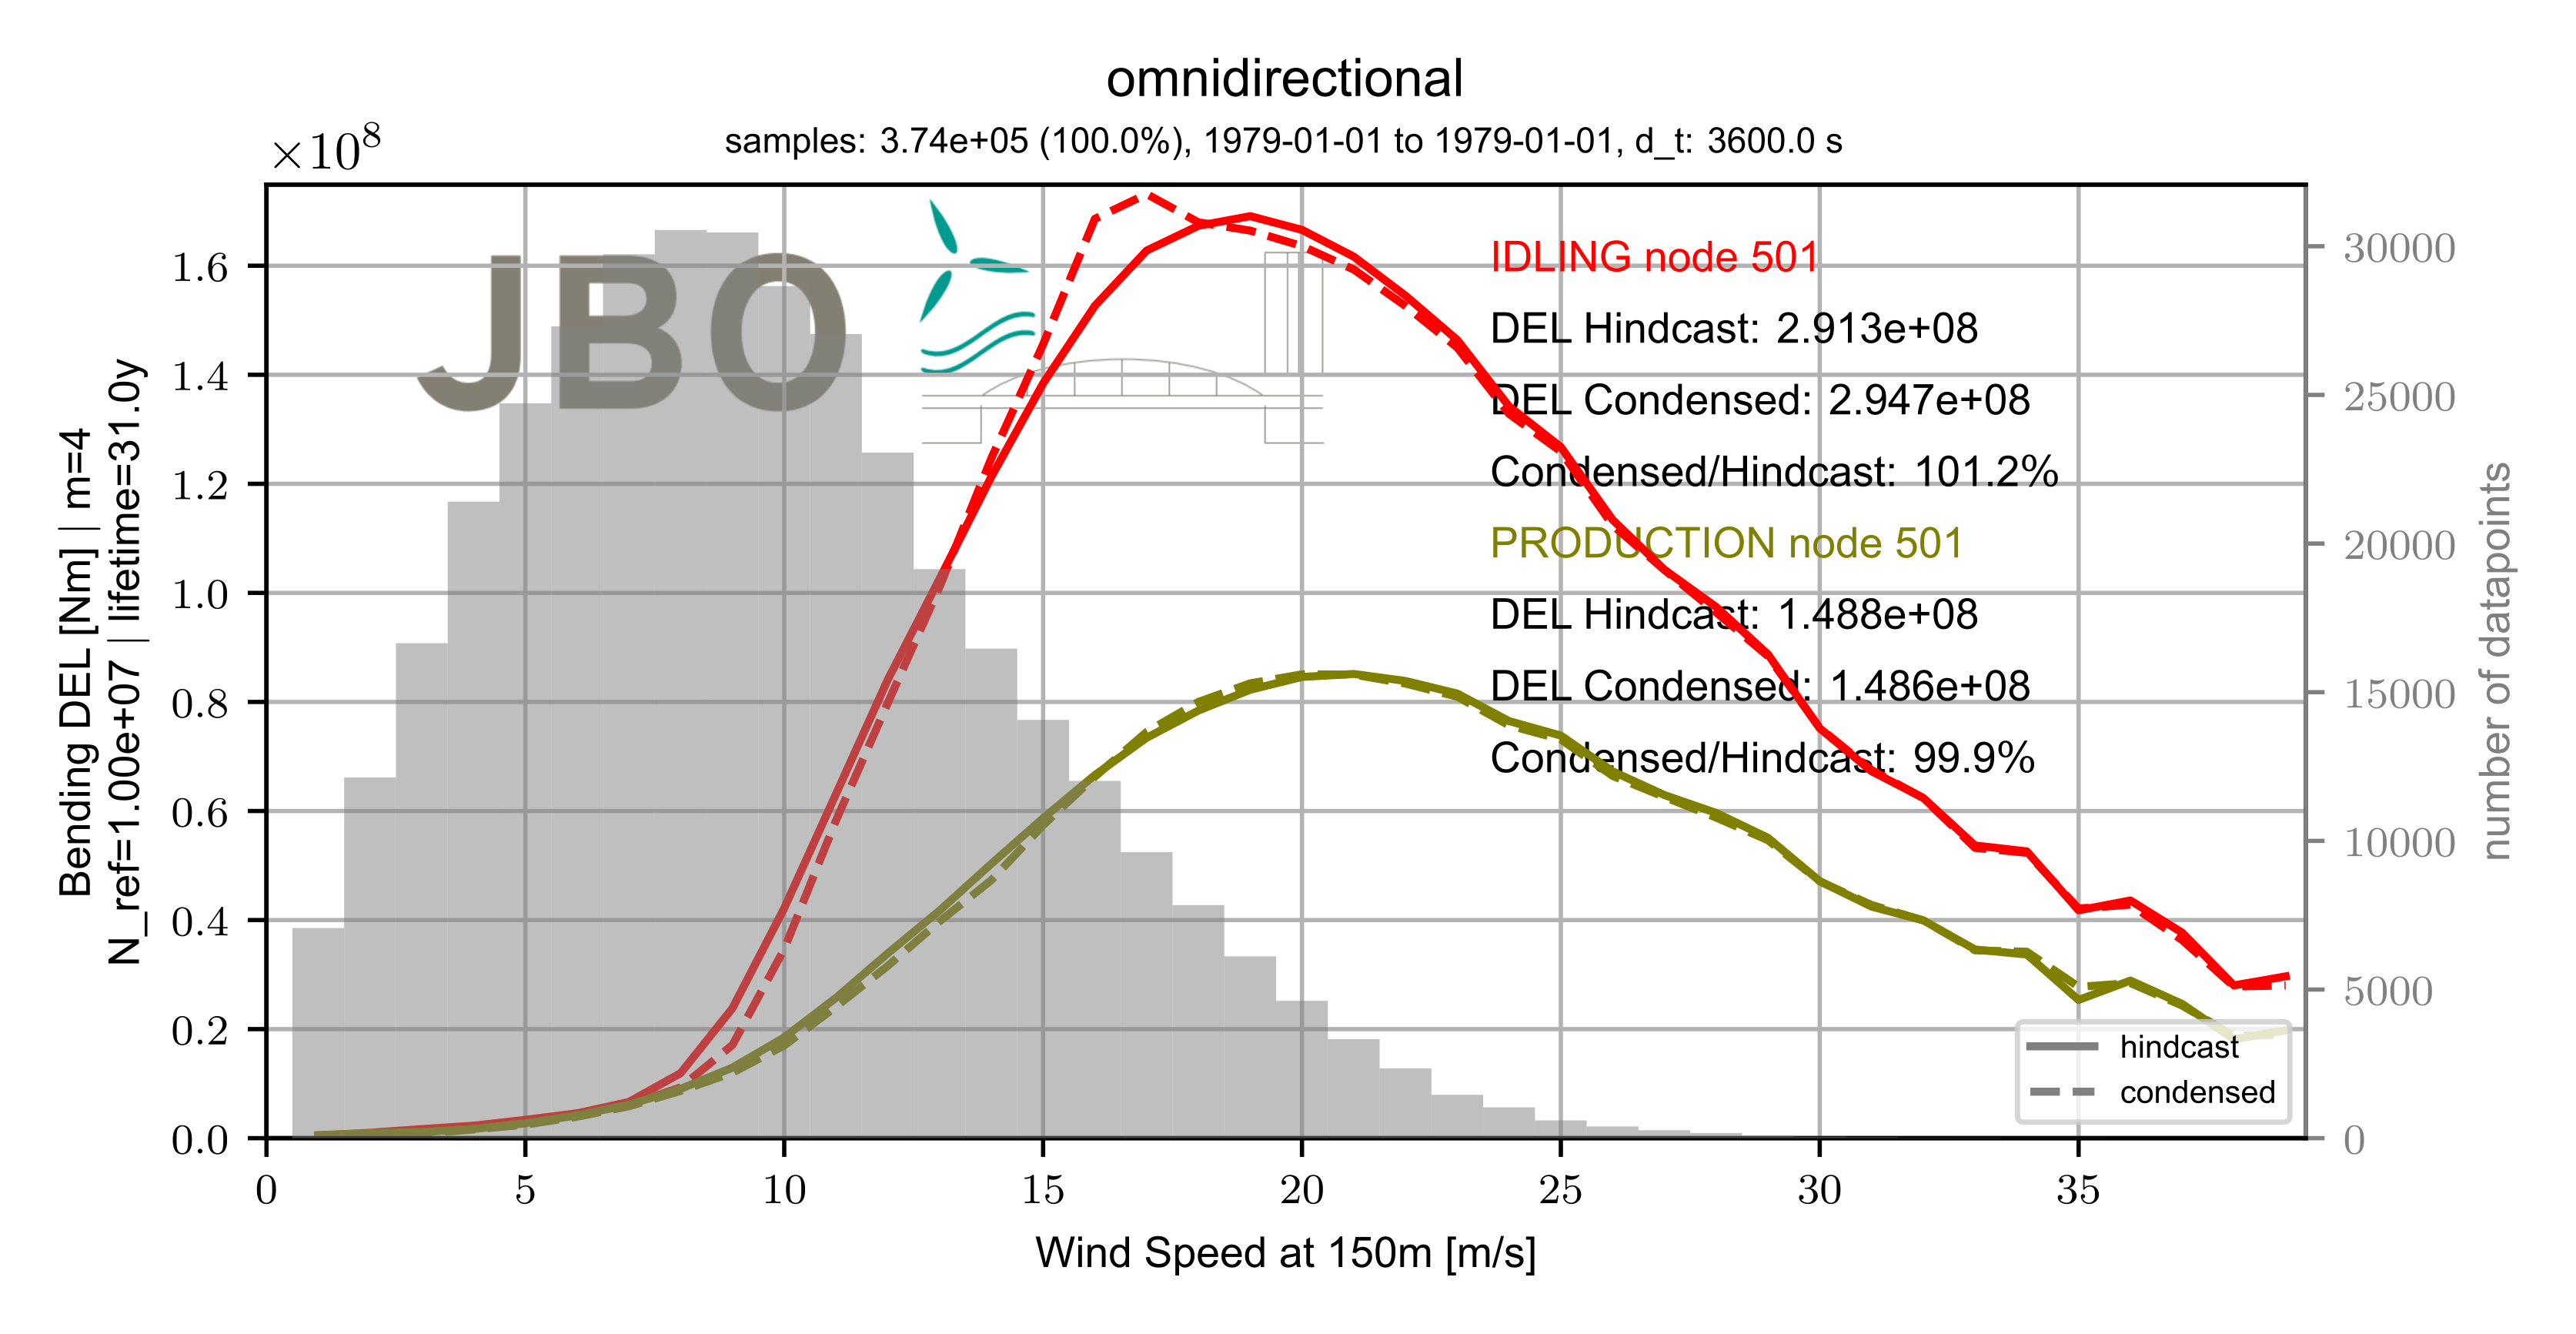
\includegraphics[width=1.0\textwidth]{C:/Users/aaron.lange/Desktop/Projekte/Hindcast_Tool/HindTool/example_output/Valid_line_wind_page_3.png} 
 \caption{ Valid-line-wind-page-3 } 
 \label{fig: Valid_line_wind_page_3 } 
\end{figure}

\begin{figure}[H] 
 \centering 
 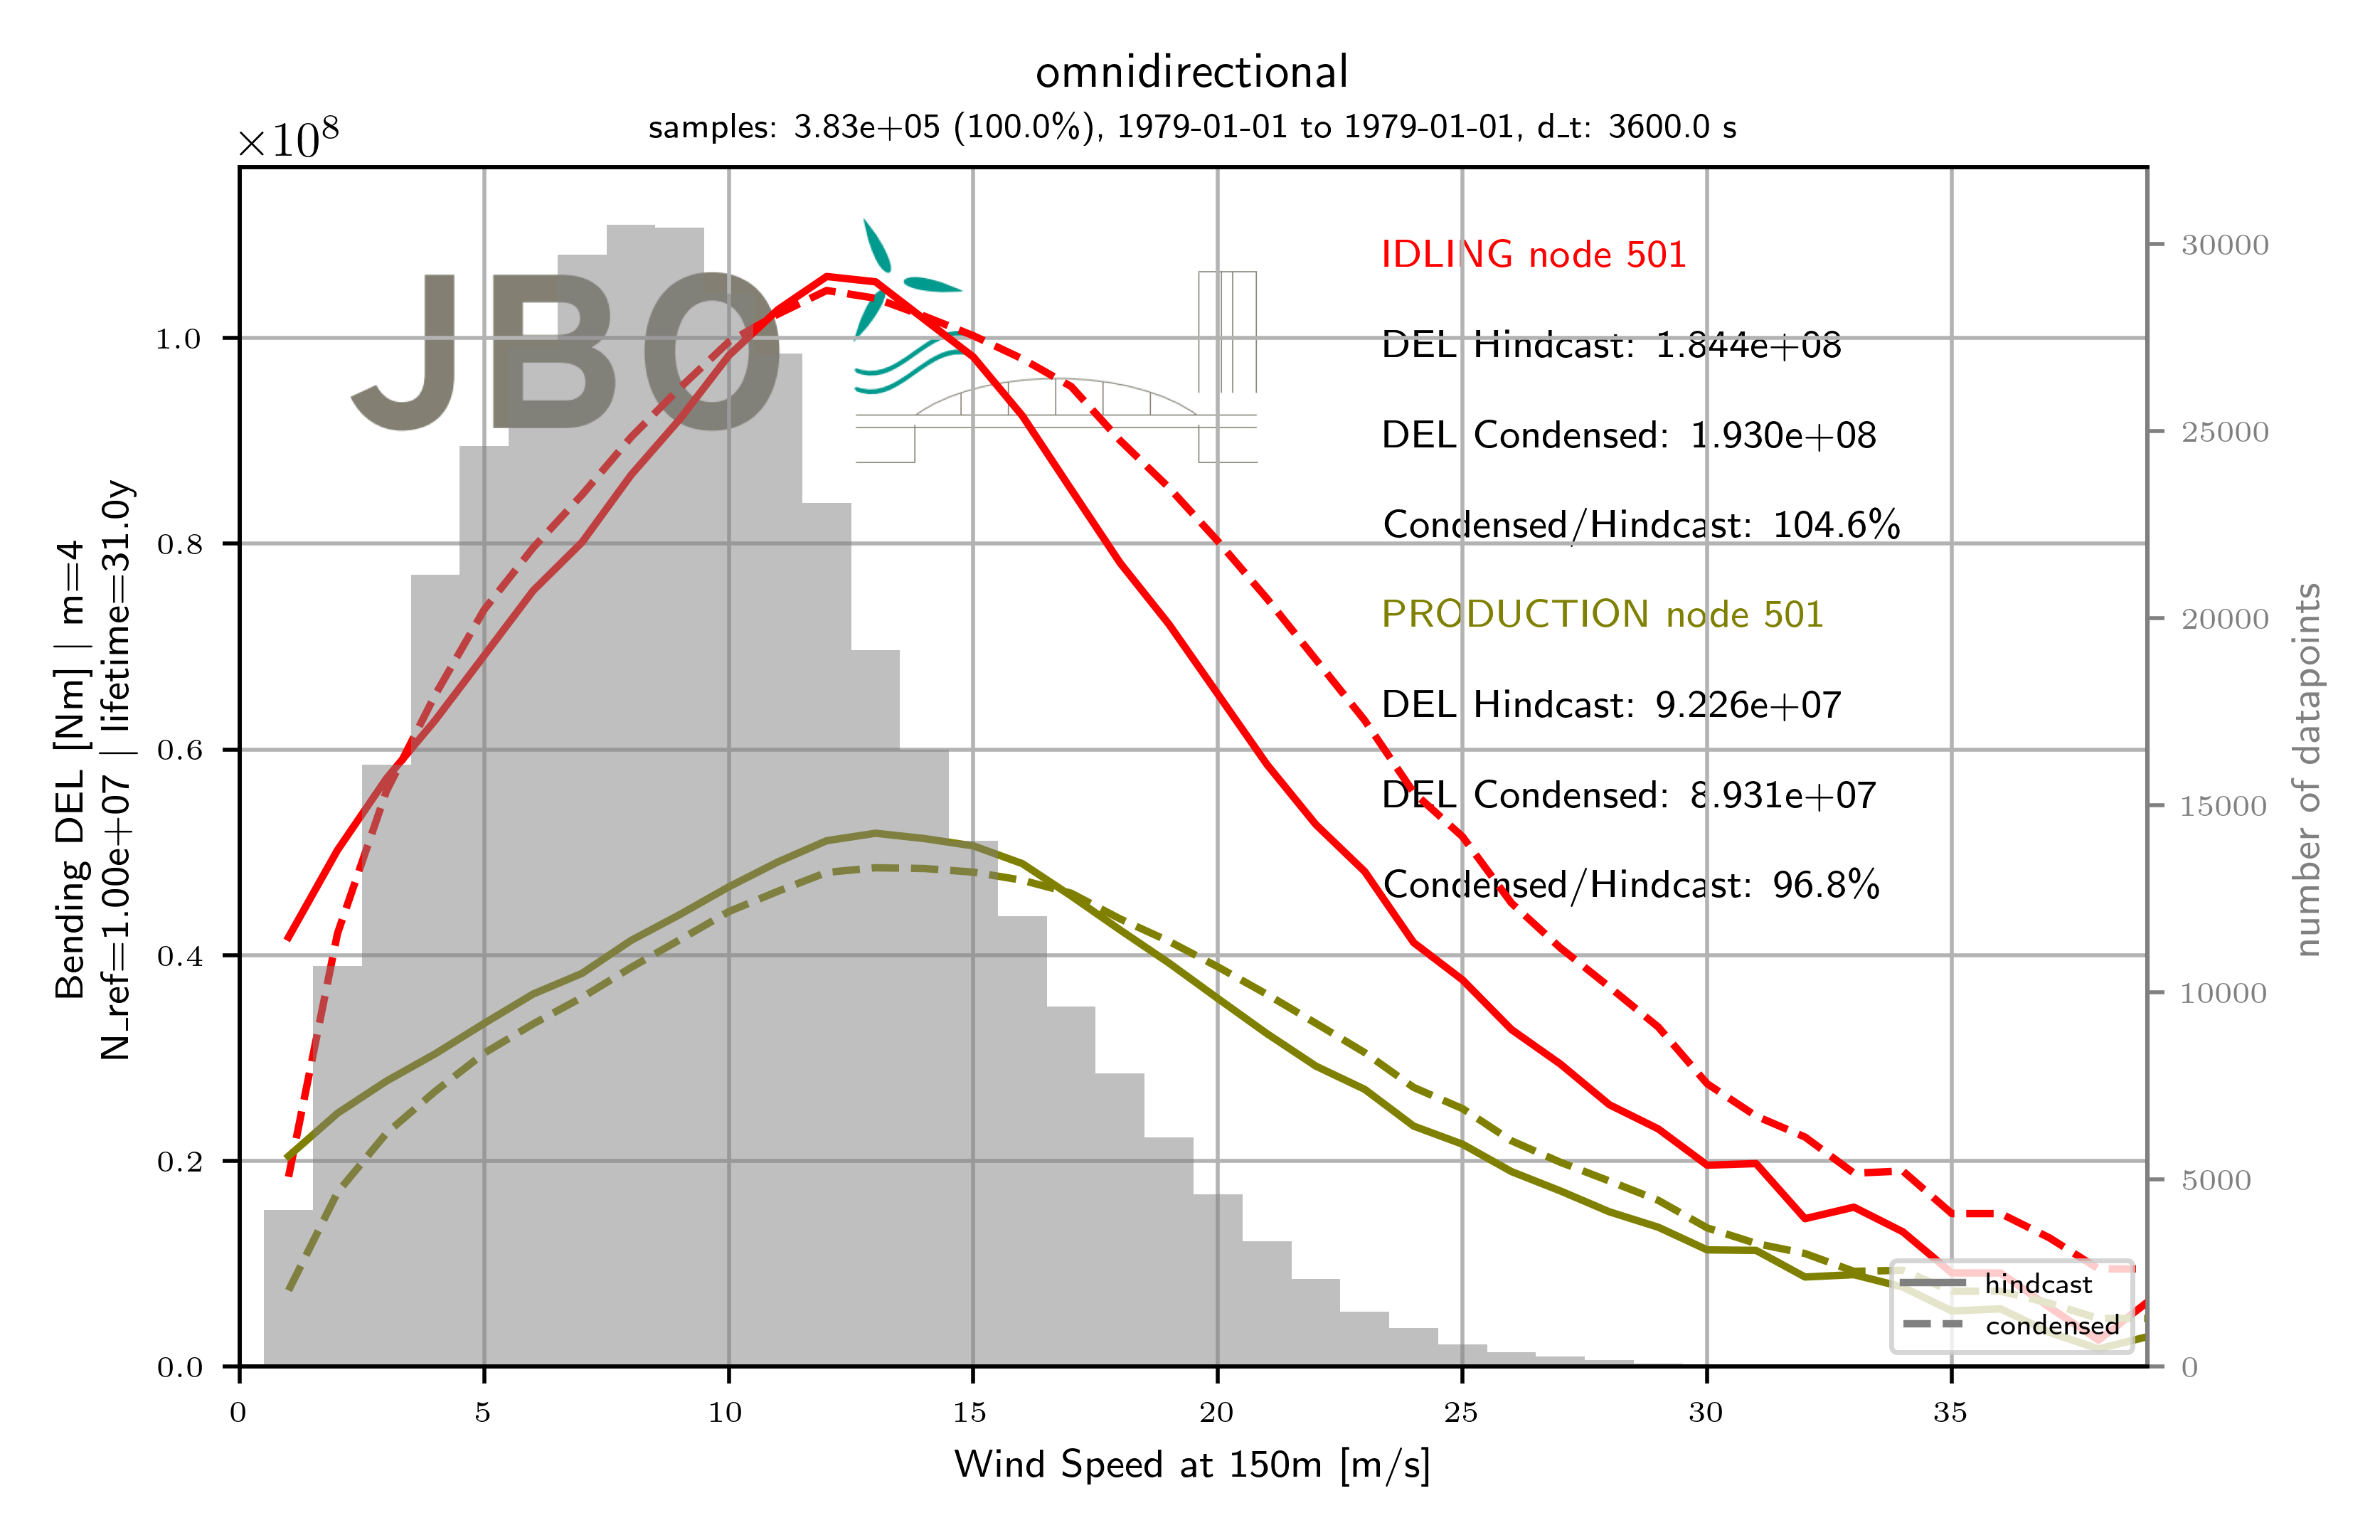
\includegraphics[width=1.0\textwidth]{C:/Users/aaron.lange/Desktop/Projekte/Hindcast_Tool/HindTool/example_output/Valid_line_swell_page_3.png} 
 \caption{ Valid-line-swell-page-3 } 
 \label{fig: Valid_line_swell_page_3 } 
\end{figure}

\begin{figure}[H] 
 \centering 
 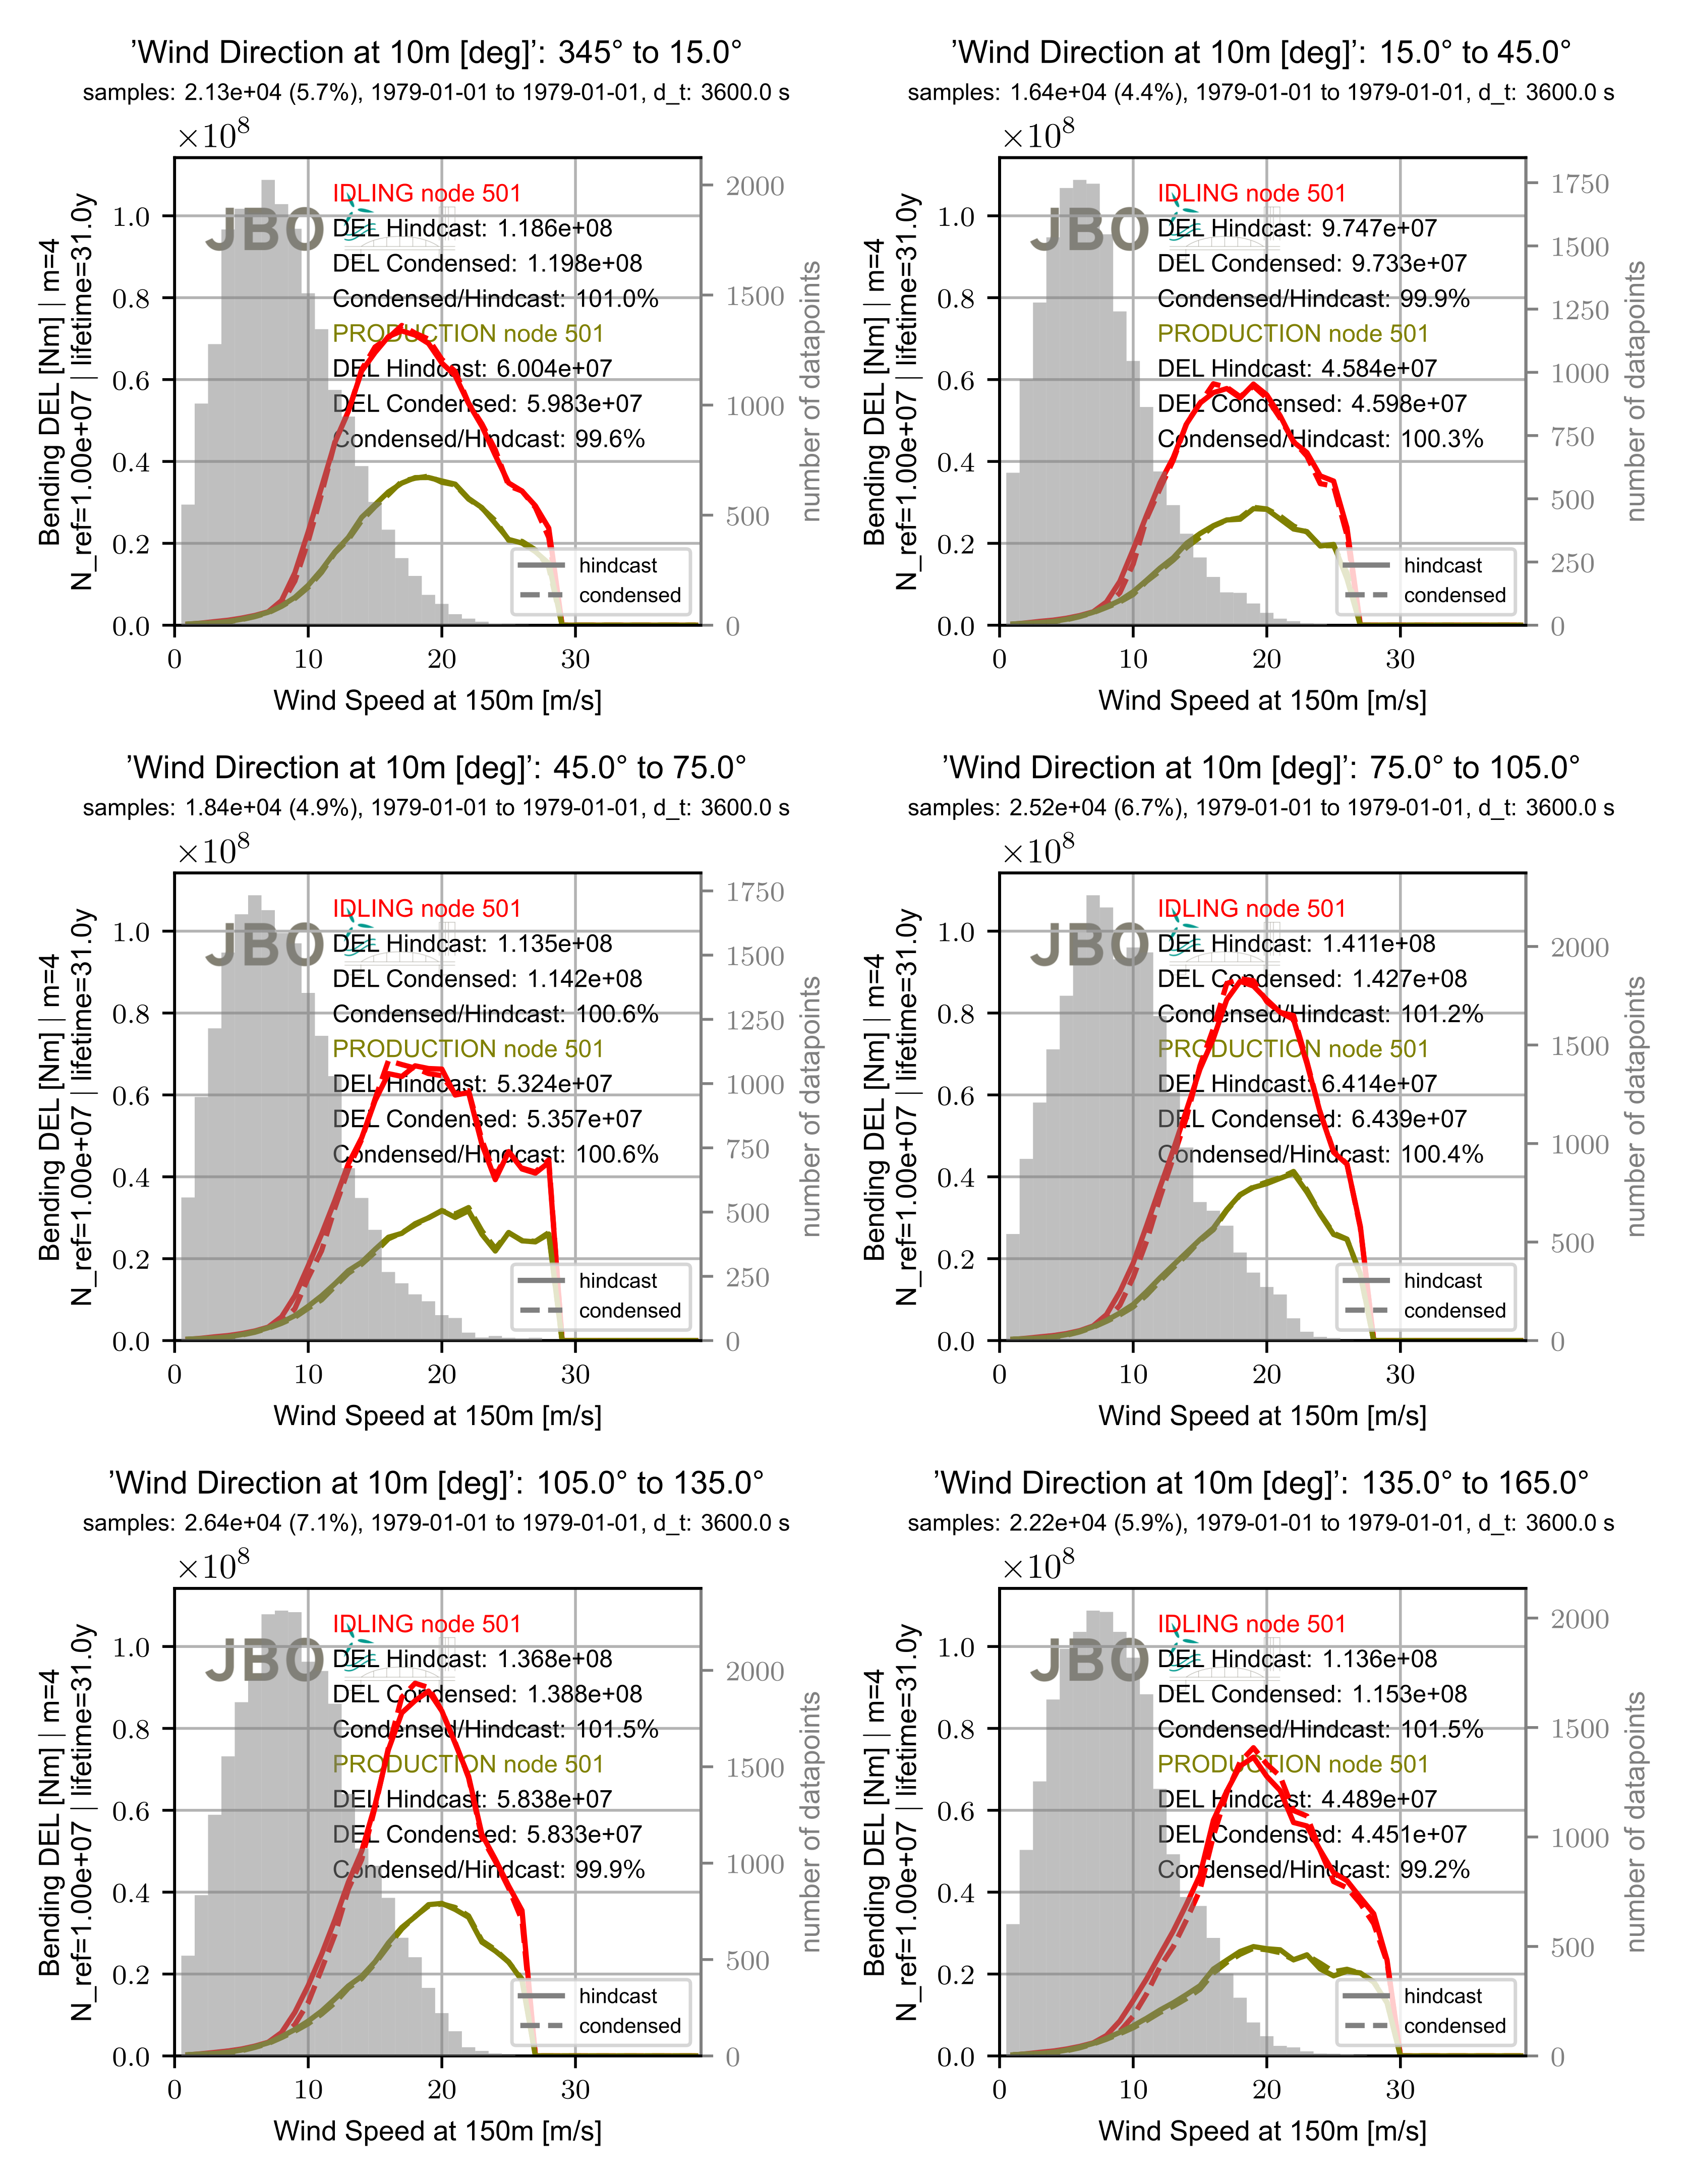
\includegraphics[width=1.0\textwidth]{C:/Users/aaron.lange/Desktop/Projekte/Hindcast_Tool/HindTool/example_output/Valid_line_wind_page_1.png} 
 \caption{ Valid-line-wind-page-1 } 
 \label{fig: Valid_line_wind_page_1 } 
\end{figure}
\begin{figure}[H] 
 \centering 
 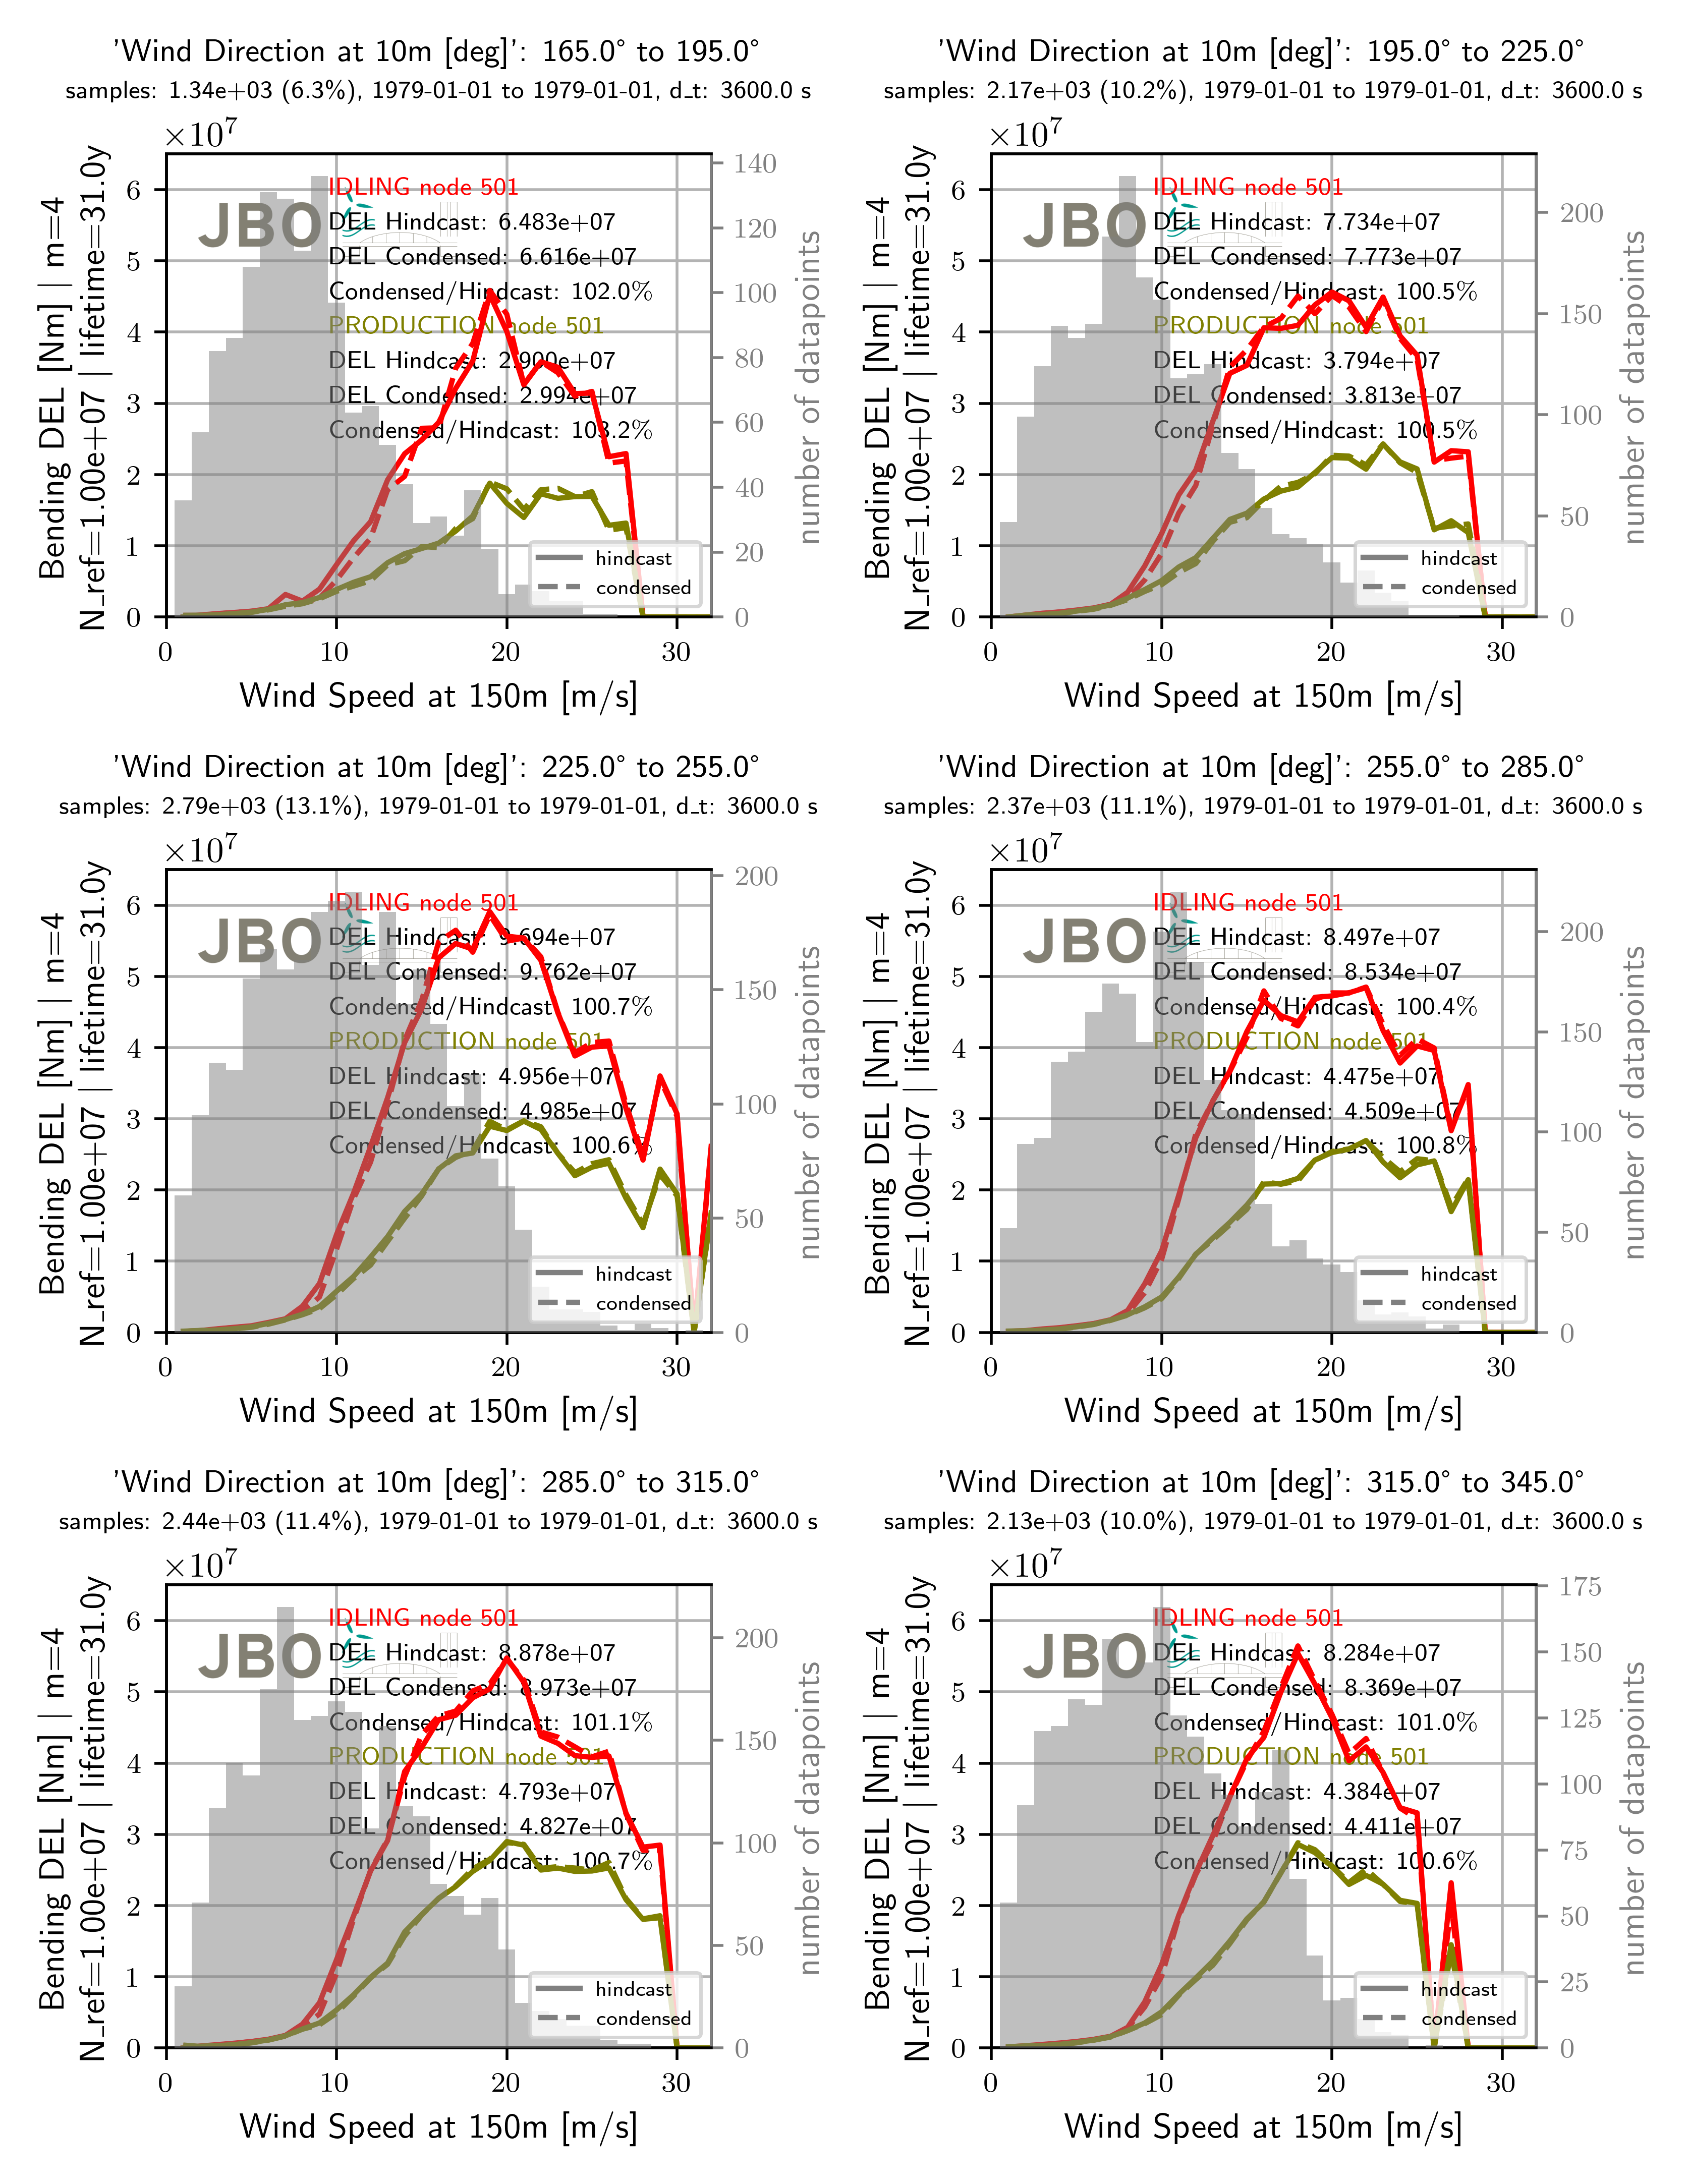
\includegraphics[width=1.0\textwidth]{C:/Users/aaron.lange/Desktop/Projekte/Hindcast_Tool/HindTool/example_output/Valid_line_wind_page_2.png} 
 \caption{ Valid-line-wind-page-2 } 
 \label{fig: Valid_line_wind_page_2 } 
\end{figure}
\begin{figure}[H] 
 \centering 
 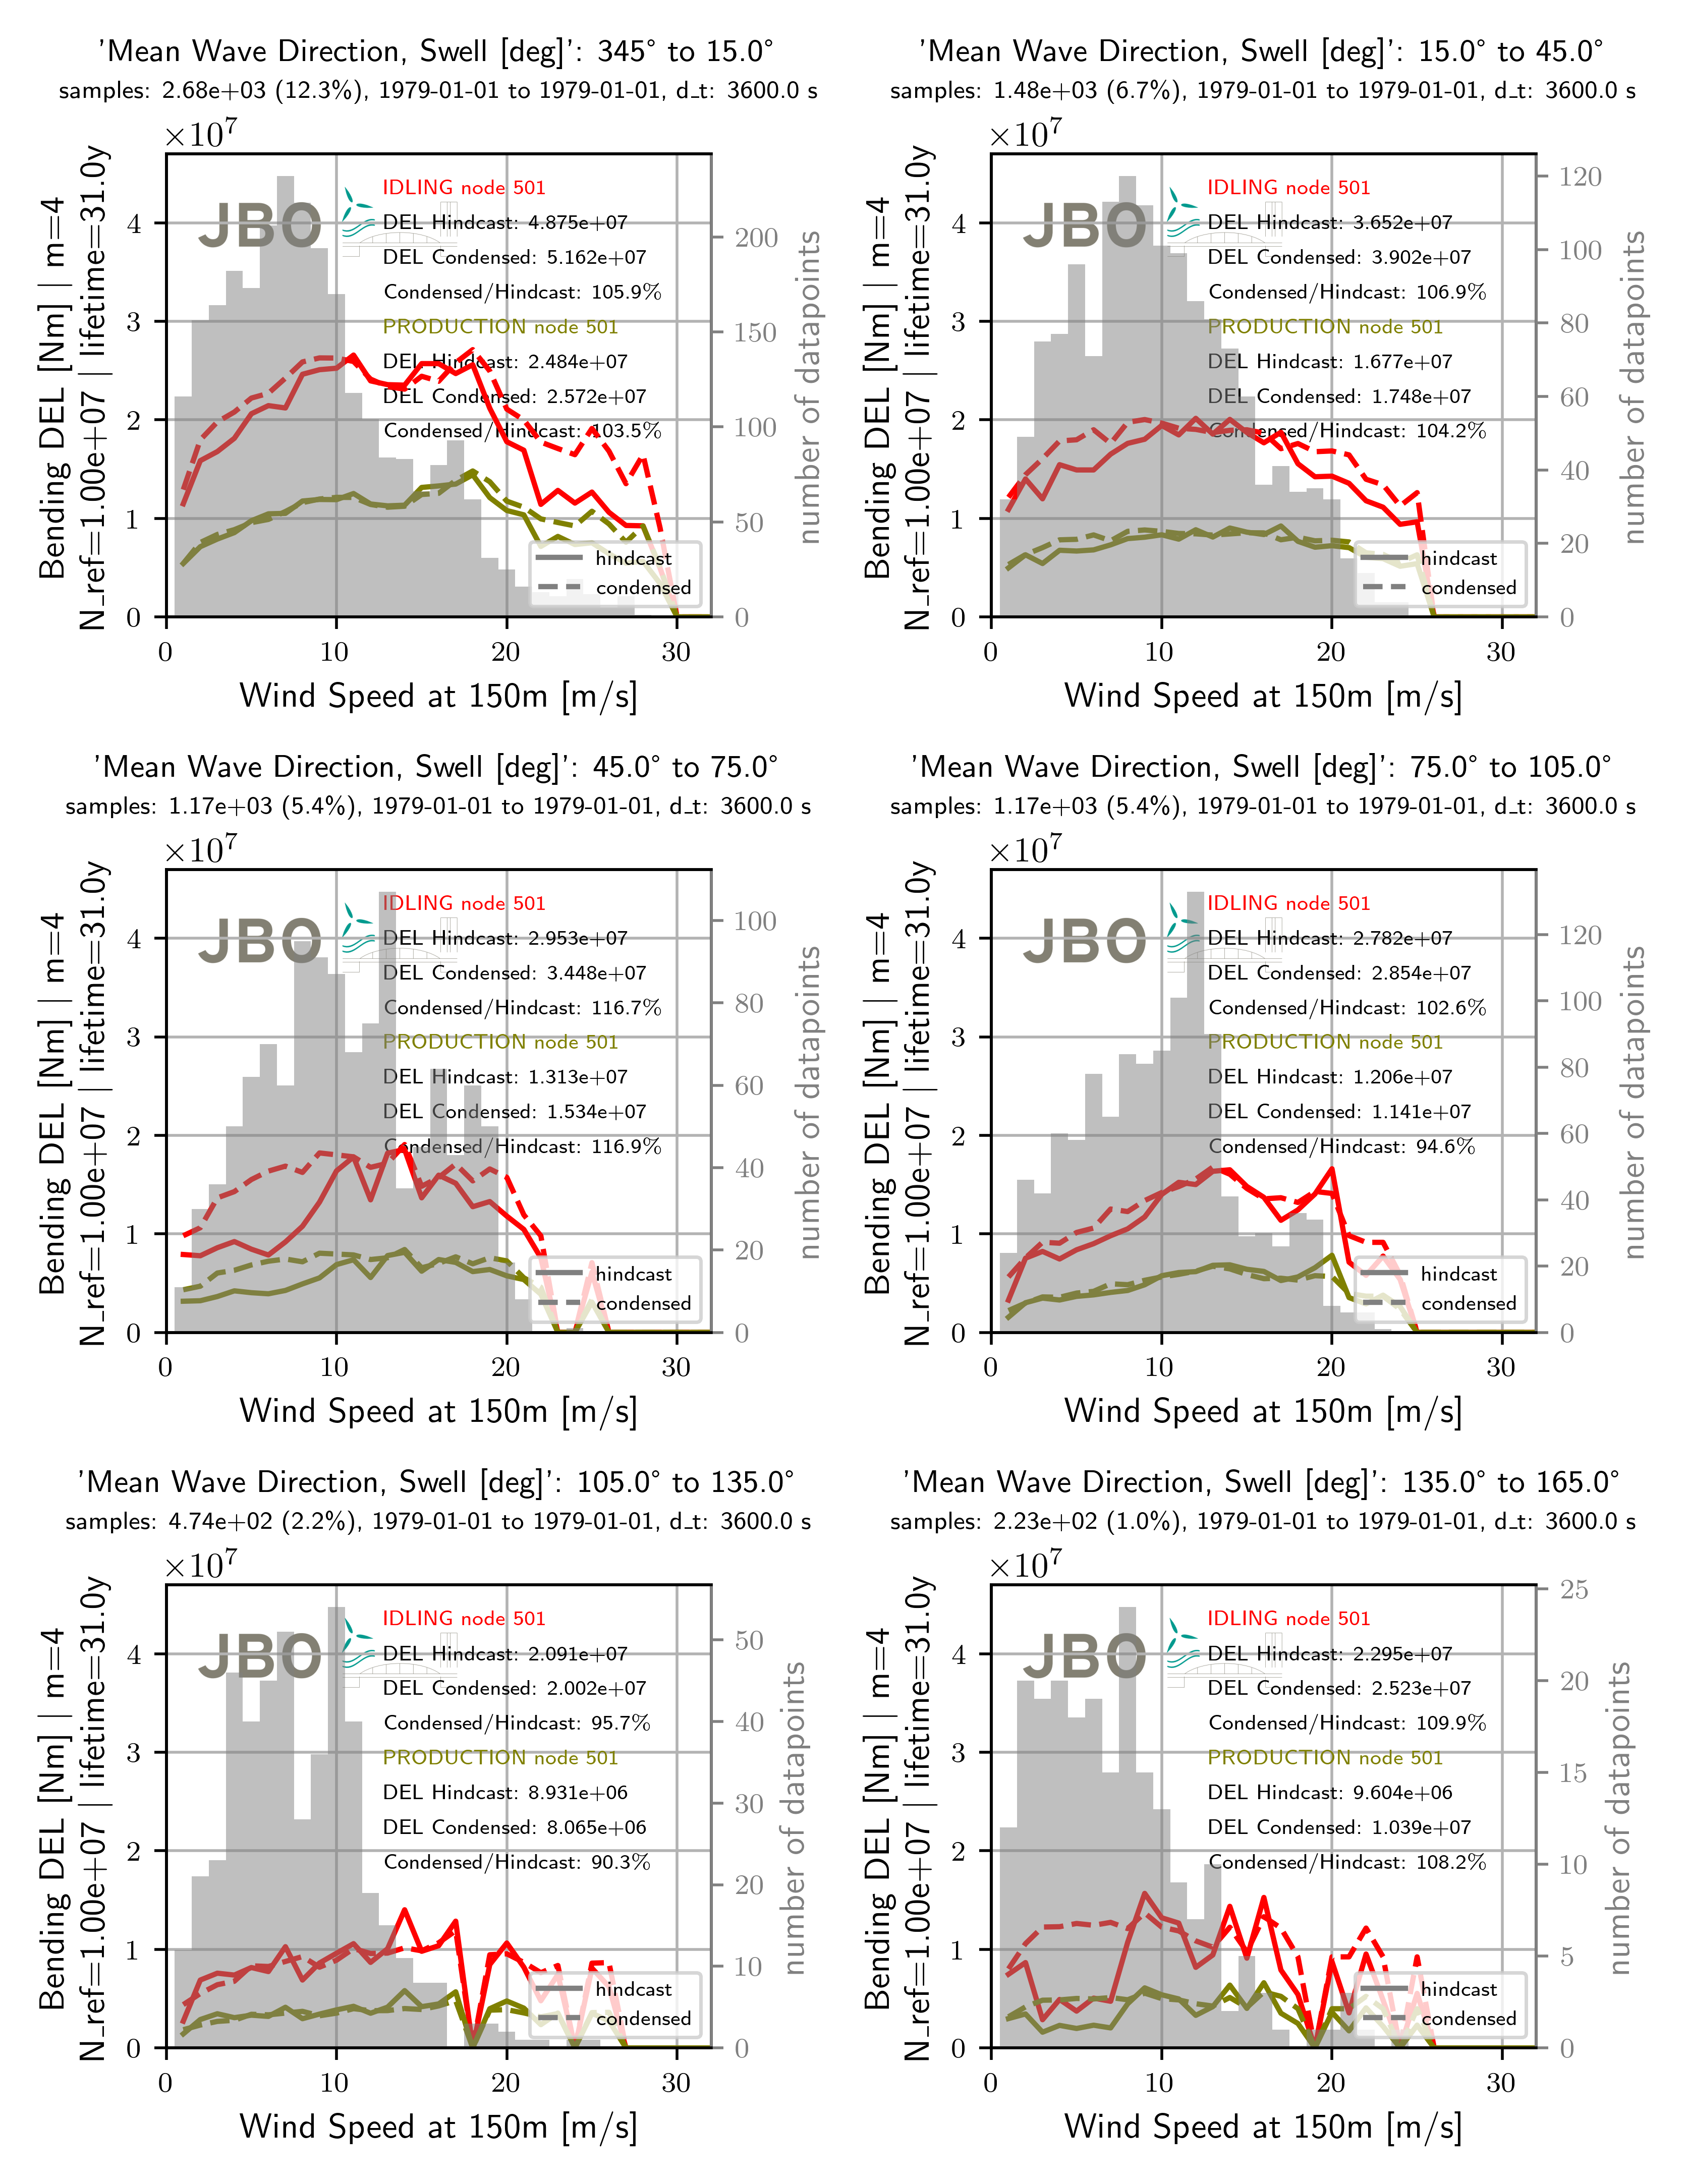
\includegraphics[width=1.0\textwidth]{C:/Users/aaron.lange/Desktop/Projekte/Hindcast_Tool/HindTool/example_output/Valid_line_swell_page_1.png} 
 \caption{ Valid-line-swell-page-1 } 
 \label{fig: Valid_line_swell_page_1 } 
\end{figure}
\begin{figure}[H] 
 \centering 
 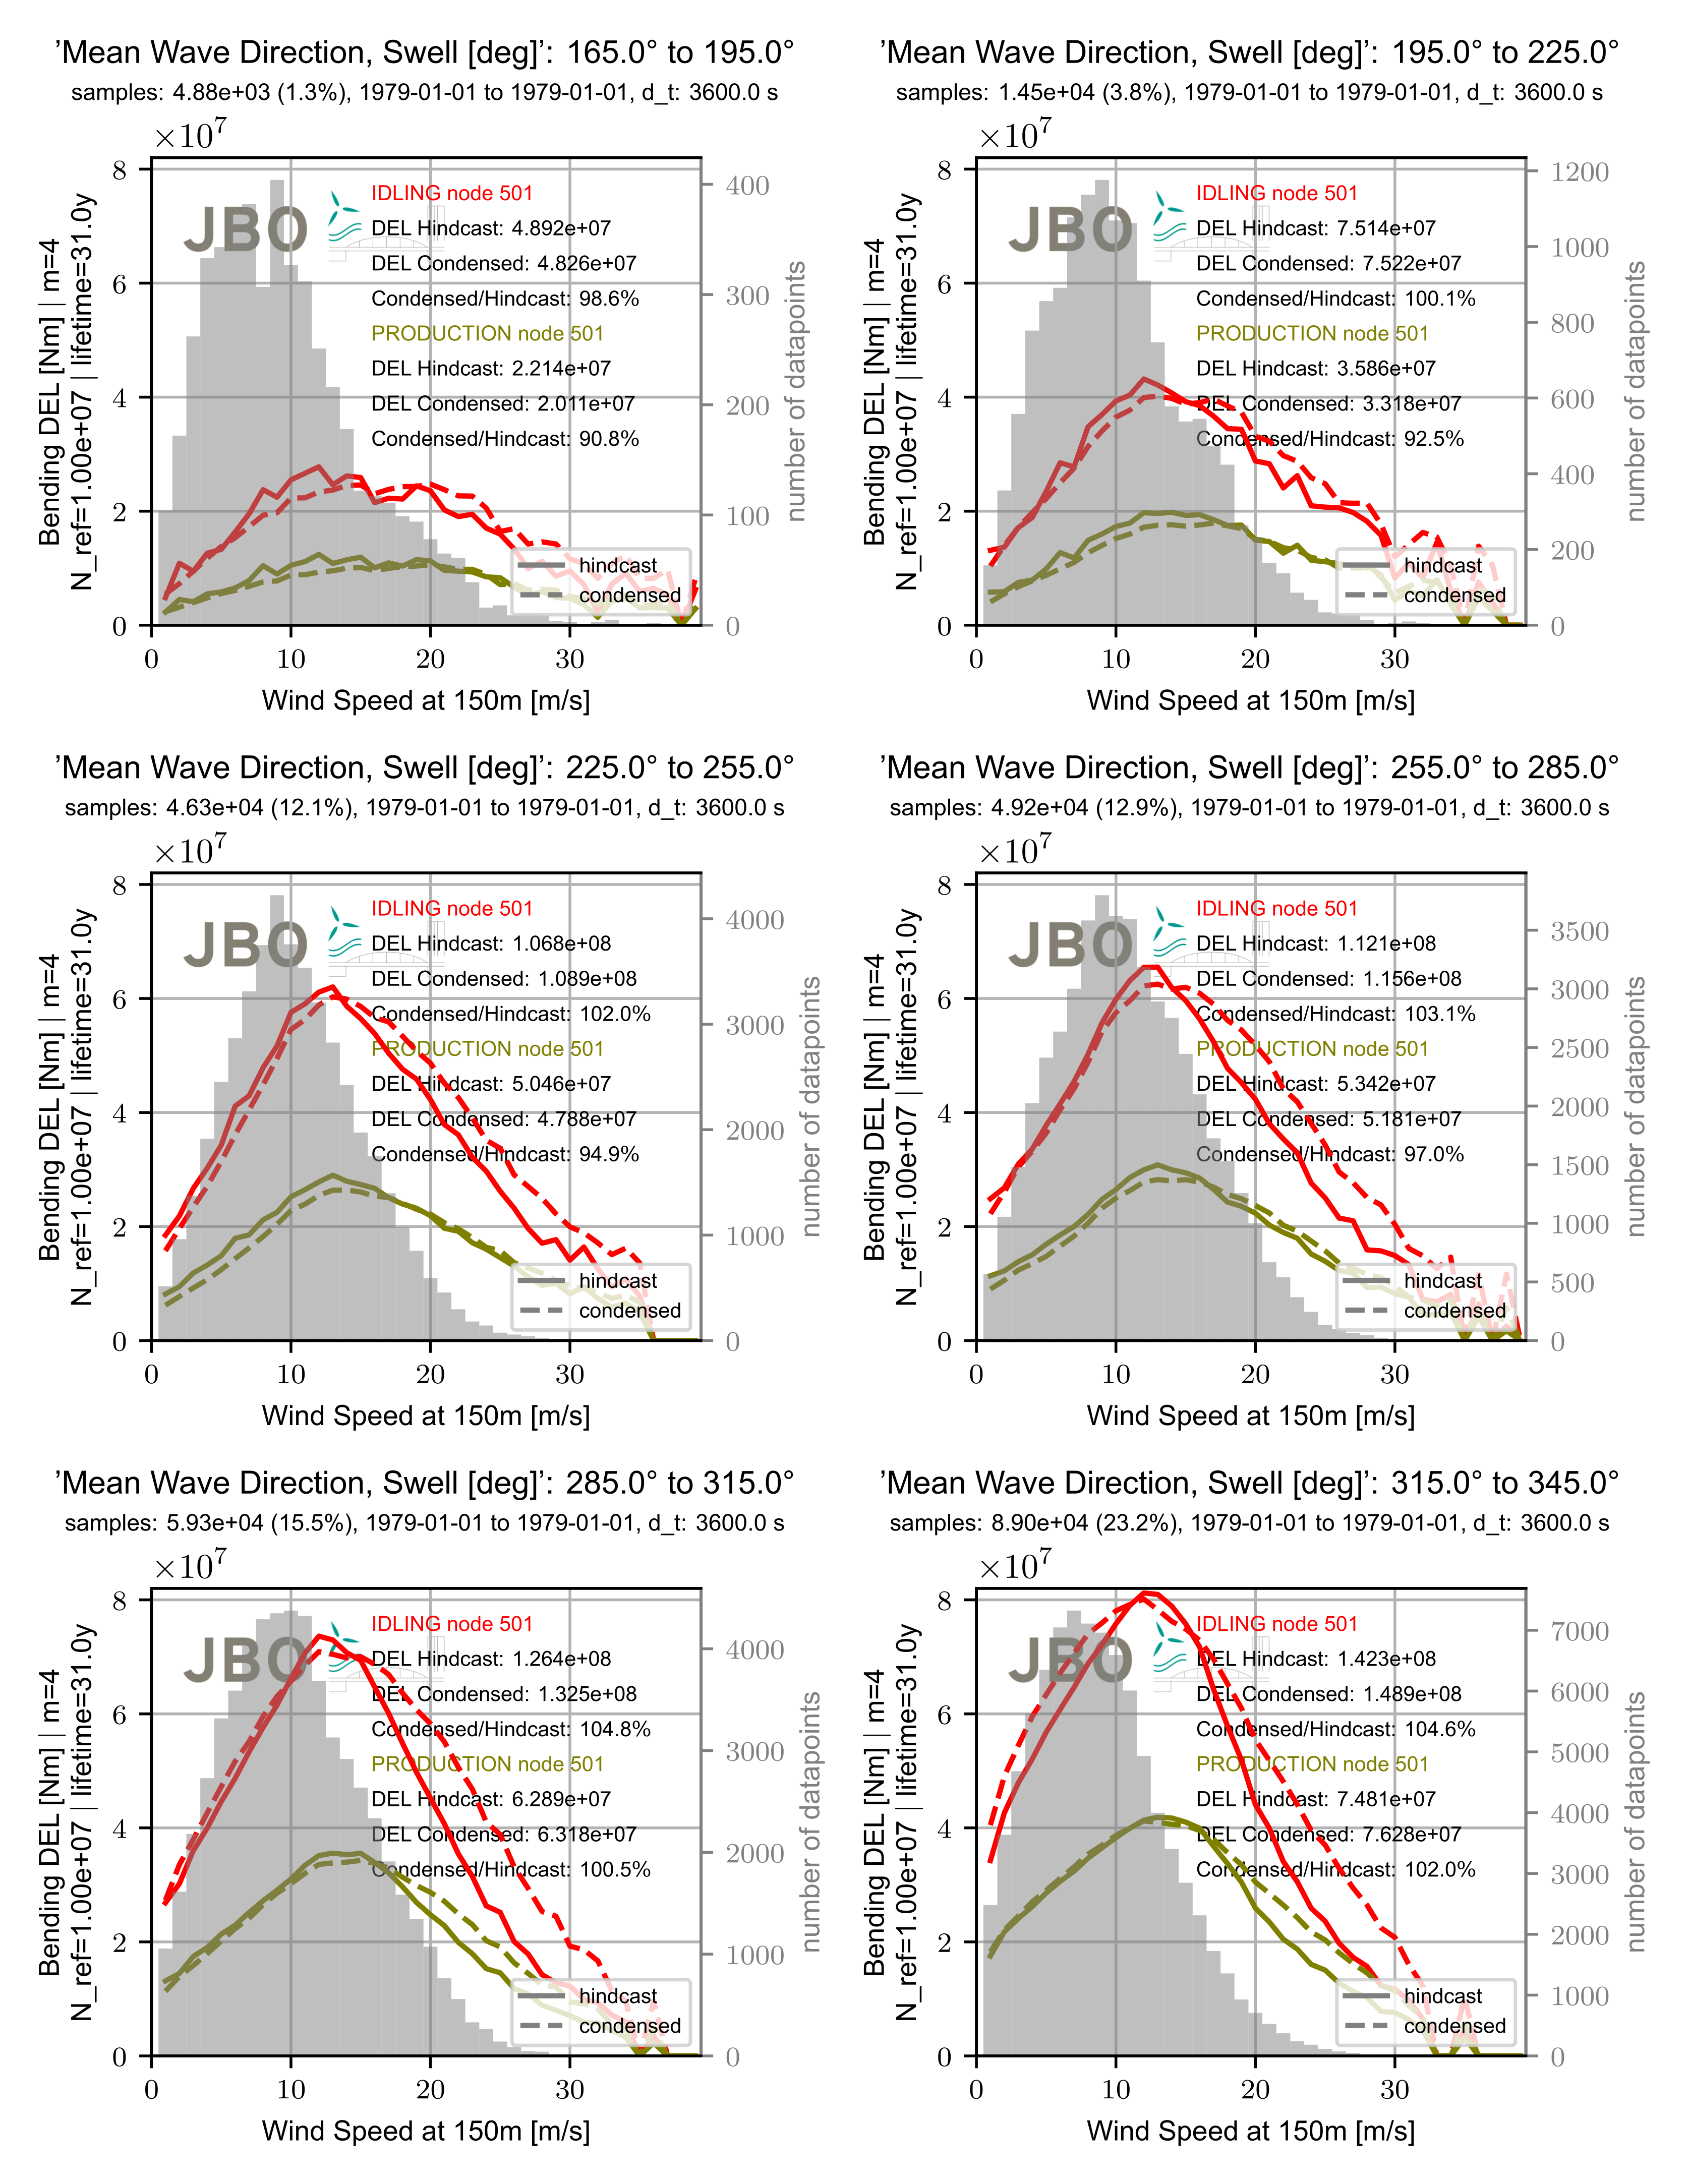
\includegraphics[width=1.0\textwidth]{C:/Users/aaron.lange/Desktop/Projekte/Hindcast_Tool/HindTool/example_output/Valid_line_swell_page_2.png} 
 \caption{ Valid-line-swell-page-2 } 
 \label{fig: Valid_line_swell_page_2 } 
\end{figure}
\begin{figure}[H] 
 \centering 
 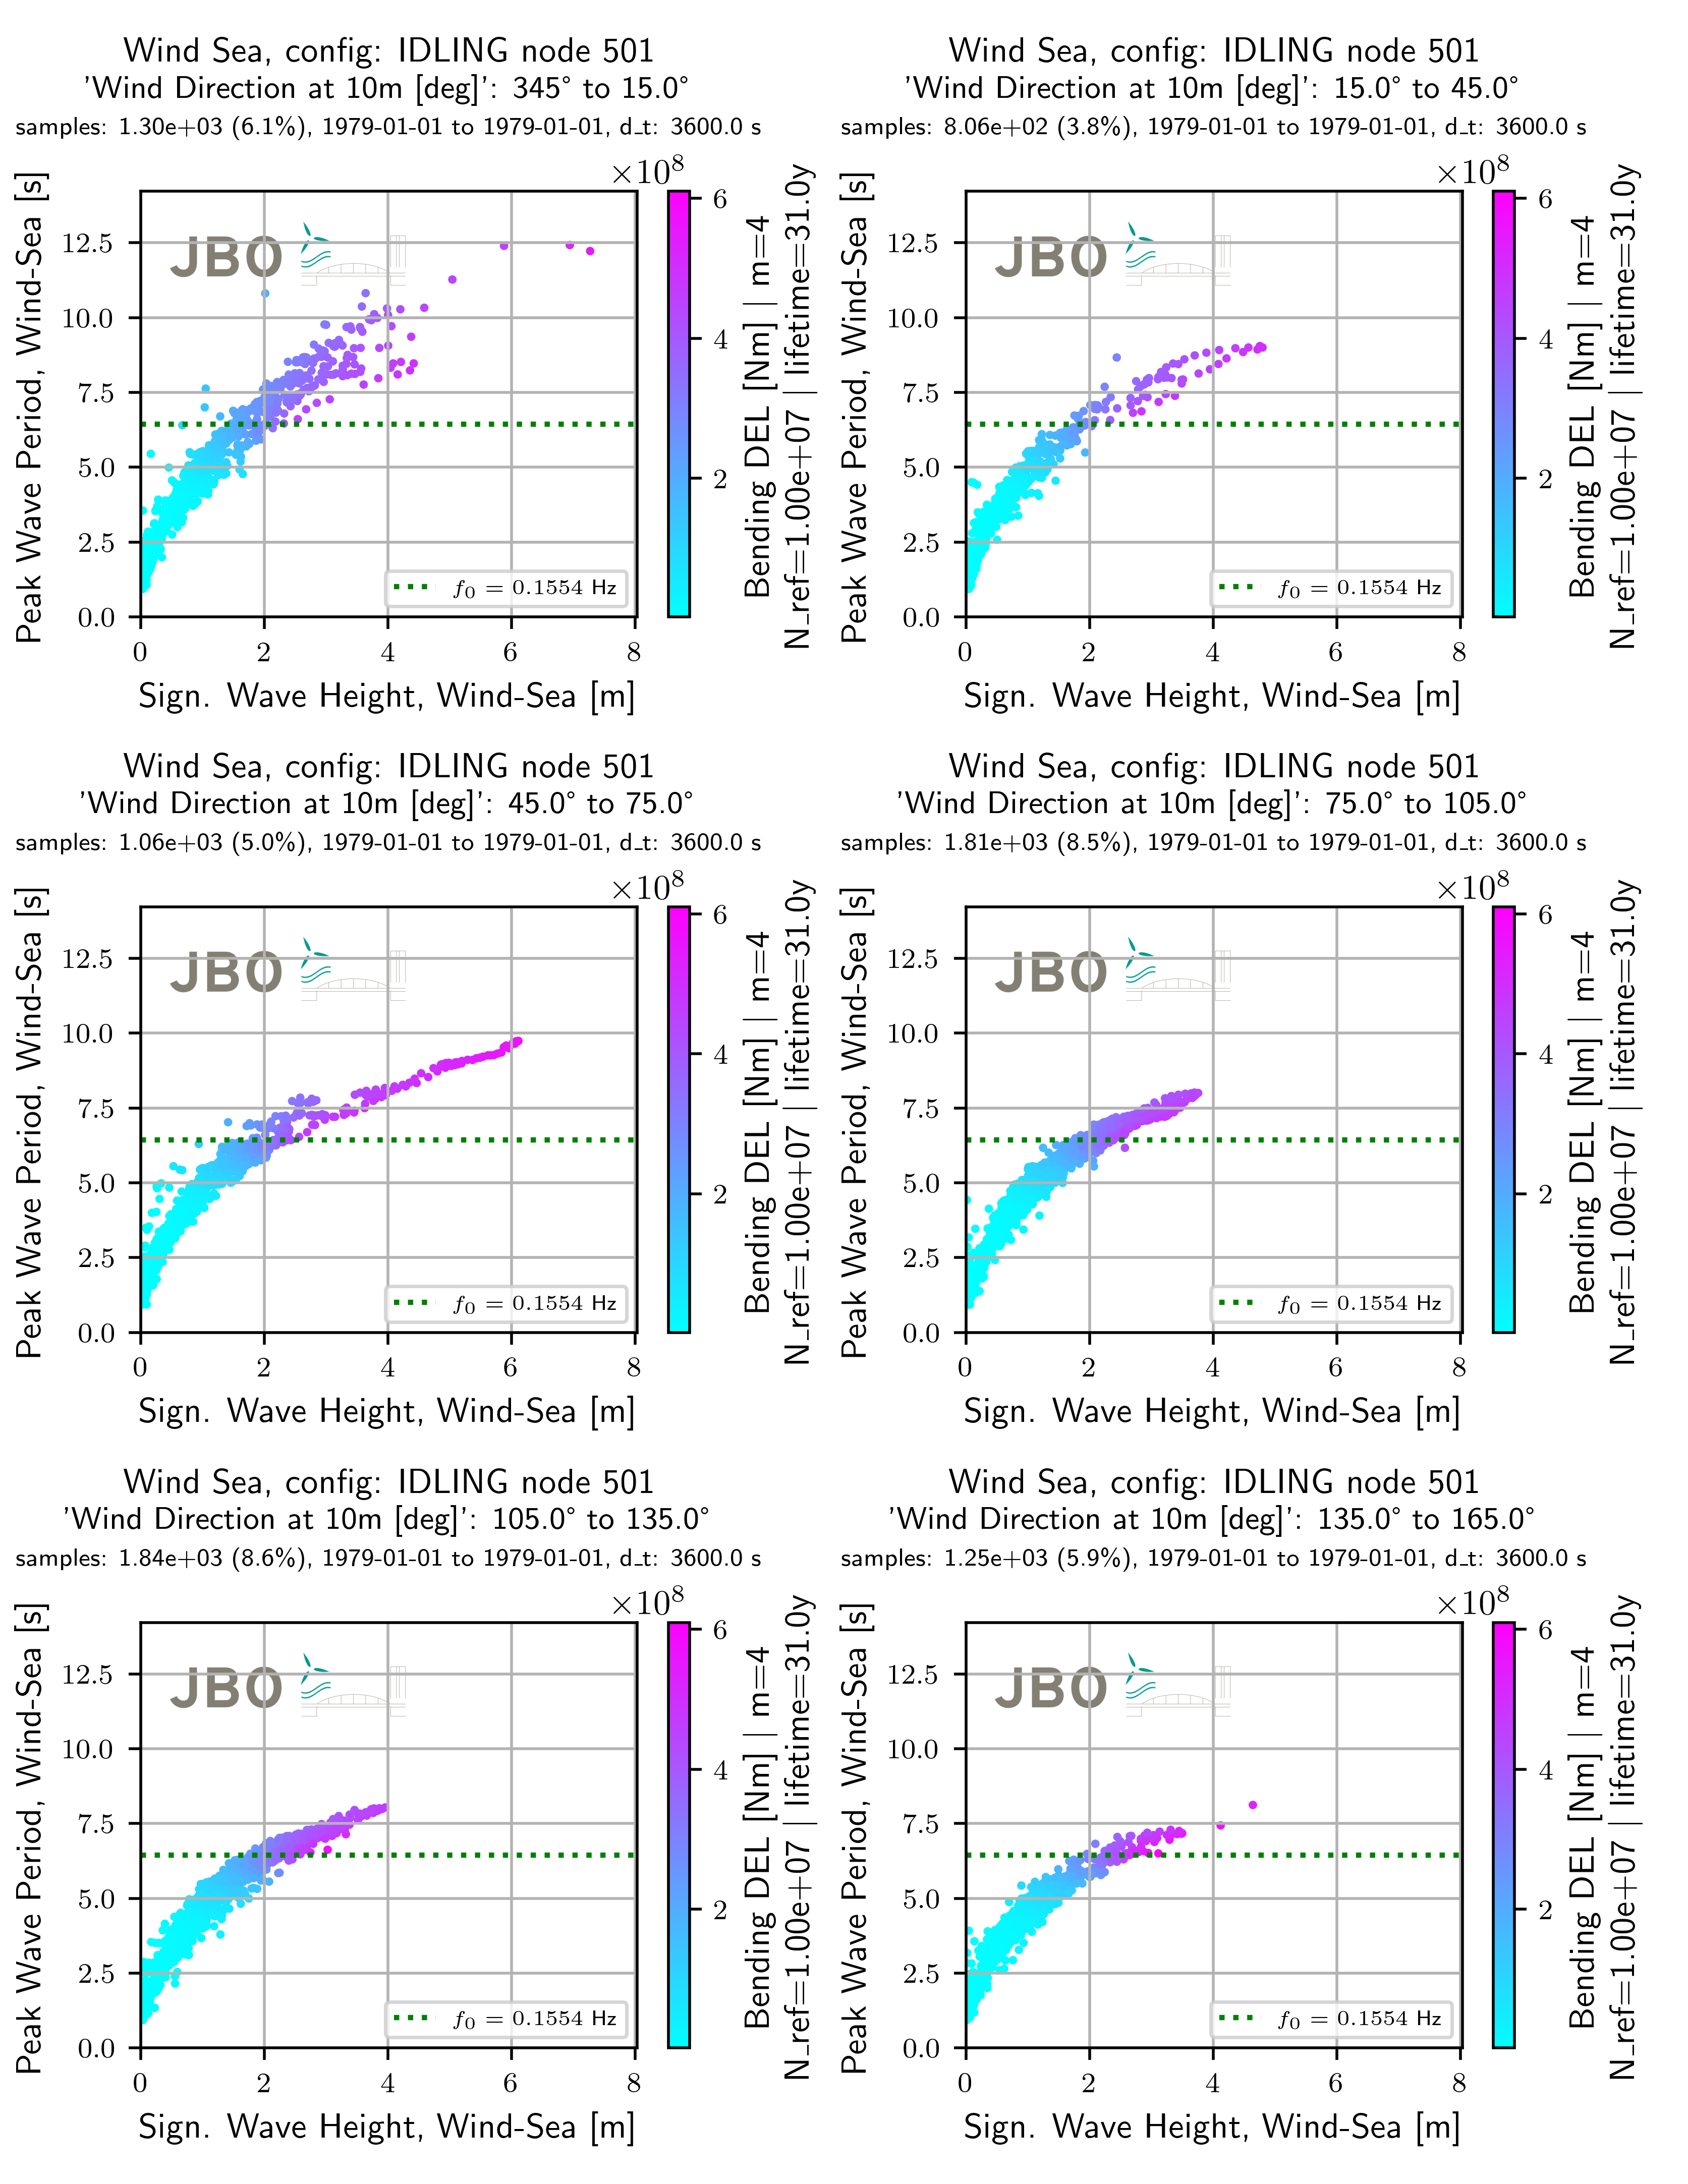
\includegraphics[width=1.0\textwidth]{C:/Users/aaron.lange/Desktop/Projekte/Hindcast_Tool/HindTool/example_output/Valid_scatter_wind_page_1.png} 
 \caption{ Valid-scatter-wind-page-1 } 
 \label{fig: Valid_scatter_wind_page_1 } 
\end{figure}
\begin{figure}[H] 
 \centering 
 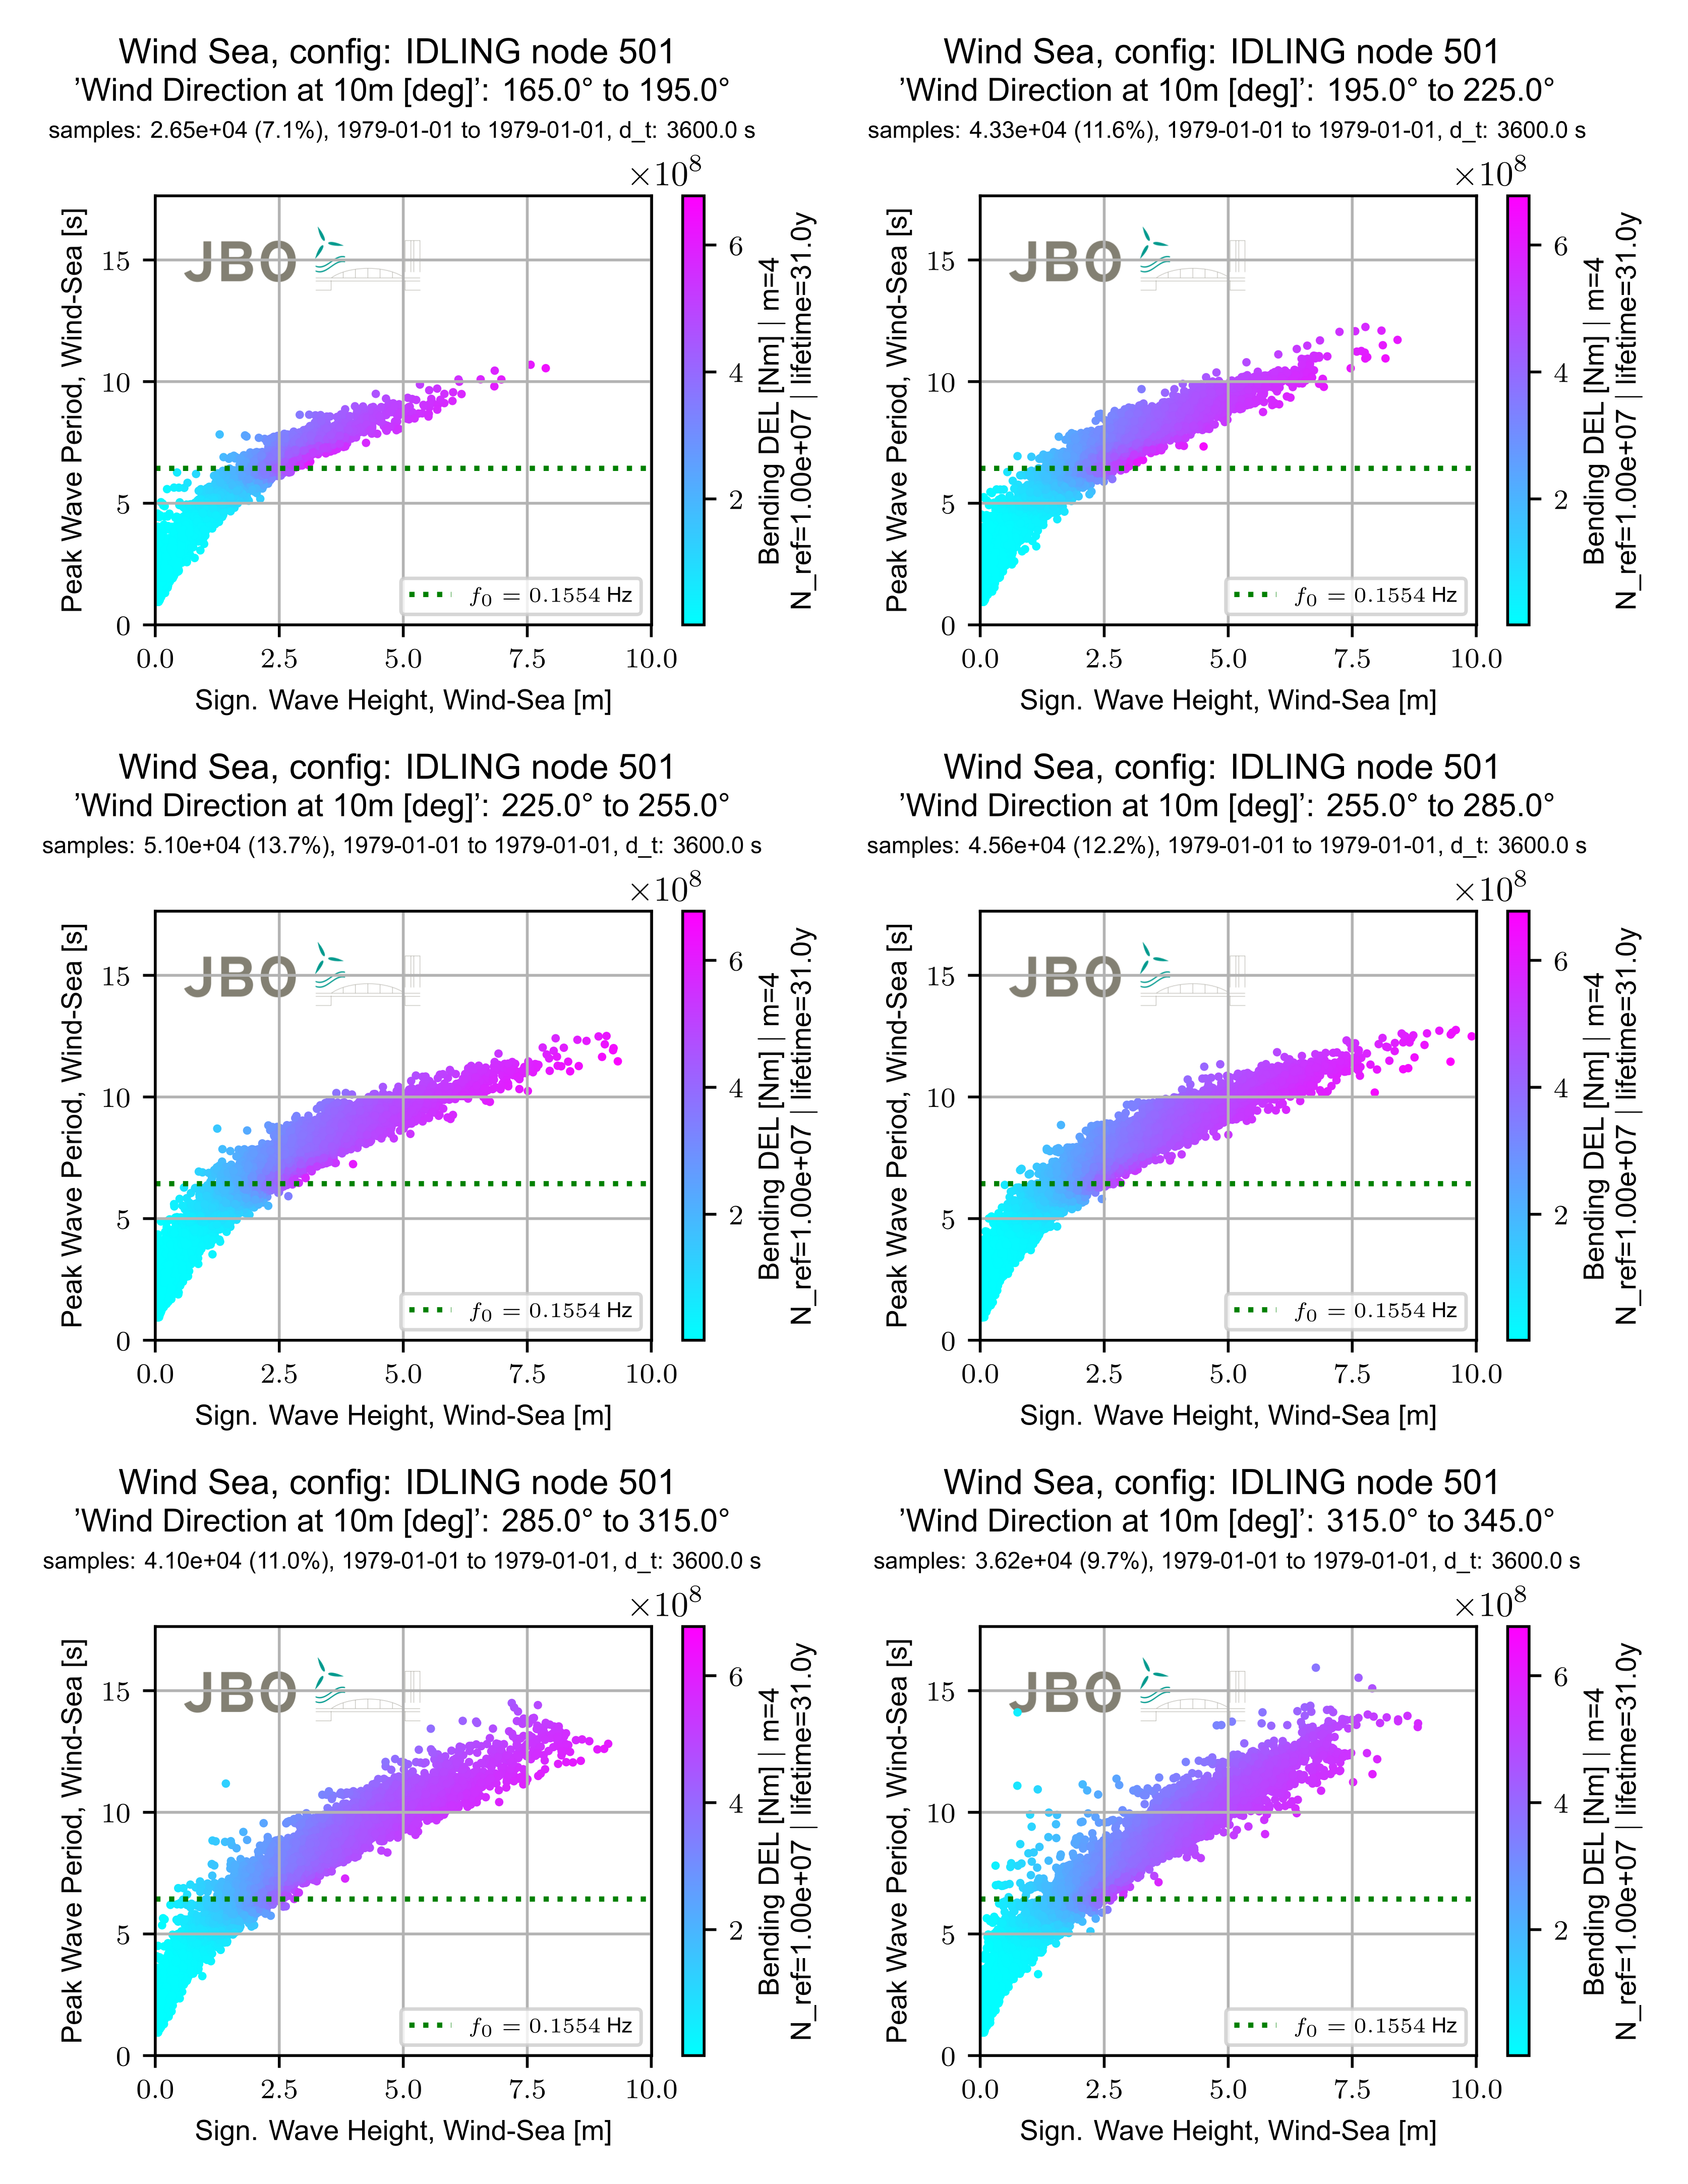
\includegraphics[width=1.0\textwidth]{C:/Users/aaron.lange/Desktop/Projekte/Hindcast_Tool/HindTool/example_output/Valid_scatter_wind_page_2.png} 
 \caption{ Valid-scatter-wind-page-2 } 
 \label{fig: Valid_scatter_wind_page_2 } 
\end{figure}
\begin{figure}[H] 
 \centering 
 \includegraphics[width=1.0\textwidth]{C:/Users/aaron.lange/Desktop/Projekte/Hindcast_Tool/HindTool/example_output/Valid_scatter_swell_page_1.png} 
 \caption{ Valid-scatter-swell-page-1 } 
 \label{fig: Valid_scatter_swell_page_1 } 
\end{figure}
\begin{figure}[H] 
 \centering 
 \includegraphics[width=1.0\textwidth]{C:/Users/aaron.lange/Desktop/Projekte/Hindcast_Tool/HindTool/example_output/Valid_scatter_swell_page_2.png} 
 \caption{ Valid-scatter-swell-page-2 } 
 \label{fig: Valid_scatter_swell_page_2 } 
\end{figure}

\section{Extreme conditions}

The extreme values for the respective occurrence periods are analysed using the Extreme Value Theory developed by Gumbel (REF). Therefore, the extreme values $x$ are determined by choosing the n maxima per year of the dataset (here, $n=1$ ). The segmentation must not be strictly at the change of the year but can be shifted by a relative offset to isolate seasonal periods with increased density of extreme values (see Figure $6-18$ ). This ensures that any two extreme values aren't correlated with each other.\\

\begin{figure}[H] 
 \centering 
 \includegraphics[width=1.0\textwidth]{C:/Users/aaron.lange/Desktop/Projekte/Hindcast_Tool/HindTool/latex_templates/Extreme_Timeseries_Example.jpg} 
 \caption{ Exemplary time series indicating extreme values on yearly separation } 
 \label{fig: Extreme_Timeseries_Example } 
\end{figure}

The Gumbel distribution considering is applied to the data set $x$ as follows:


\begin{align}
\label{eq:gumbel}
P_{G u m b}=\exp \left(-\exp \left(-\frac{x-\mu} {\beta}\right)\right) \\
\text{with: }
&\beta=\sigma \frac{\sqrt{6}}{\pi} \quad \text{(scale parameter)}\\
&\mu=\bar{x}-\gamma \beta \quad \text{(location parameter)}
\end{align}


where the standard deviation is denoted as $\sigma$, the mean value as $\bar{x}$ and the Euler-Mascheroni constant $\gamma \approx 0.5772$ . The theoretical probability $P_{t h}$ is calculated as the quantile of each of the $N$ (sorted) datapoints, following the Gumbel distribution, by using the formula:

\begin{align}
    P_{t h}=\frac{n-0.5}{N}, n=1 \ldots N
\end{align}


by finding the inverse of formula \ref{eq:gumbel}.

\begin{align}
    \label{eq:gumbel_inv}
    x_{t h}=-\beta \ln \left(-\ln P_{t h}\right)+\mu
\end{align}


Here, $n$ theoretical extreme values $x_{t h}$ are found and compared to the real extreme values $x$.

\begin{figure}[H] 
 \centering 
 \includegraphics[width=0.5\textwidth]{C:/Users/aaron.lange/Desktop/Projekte/Hindcast_Tool/HindTool/latex_templates/Extreme_qq_example.jpg} 
 \caption{ Comparison of real and theoretical extreme values } 
 \label{fig: Extreme_qq_example } 
\end{figure}

By visually evaluating the distance from a perfect correlation, shown as the line $x=x_{t h}$, the fit of the distribution can be evaluated. Also shown are the percentiles of the Gumbel distribution. These are numerically determined. $N$ uniformly distributed probabilities $p_{n} \in[0,1], n=1 \ldots N$ are generated and the corresponding theoretical extreme values are found using equation \ref{eq:gumbel}. This is repeated many times ( $N_{\text {rep }}$ ) and each of the resulting sets of size $N$ are sorted by magnitude. Now for each magnitude rank with size $N_{\text {rep }}$ any percentile can be calculated and is associated with the theoretical extreme values $x_{t h}$.

For finding the return periods $T_{R}$ corresponding to the probability value $P$ or vice versa, the formulas below can be applied (see $[\mathrm{N} 1]$ ).

\begin{align}
\label{eq:P_to_TR}
   P=\left(1-\frac{1}{n T_{R}}\right) \quad T_{R}=\frac{1}{(1-P) n}
\end{align}


Starting from a return period, Eq. \ref{eq:P_to_TR} can be used to the probability P. From there, the inverse Gumbel distribution (Eq. \ref{eq:gumbel_inv}) can be used to determine the expected extreme value. Therefore, a logarithmic grid of return periods in the required range $T_{R, j}, j=1 \ldots M$ is created and the corresponding theoretical extreme values $x_{j, m i d}$ are determined.

For finding the confidence intervals, labelled $x_{j, \sigma}$ and $x_{j,-\sigma}$, another numerical method is applied. For each of the $i$ determined sets $p_{n}$, new Gumbel coefficients $\beta_{i}$ and $\sigma_{i}$ are calculated. For each of the return periods $T_{R, j}$, the corresponding probabilities $P_{j}$ of the current Gumbel distribution are found. The result is a $N_{r e p}$ by $M$ matrix, in which there are a big number ( $N_{r e p}$ ) of extreme values corresponding to the return periods $T_{R, j}$ on the logarithmic grid. Those can be used to determine the standard deviation $\sigma_{j}$ for each of the $j$ return periods $T_{R, j}$. As suggested in REF, these values can be simply added or subtracted to the appropriate value $x_{j, m i d}$ :

$$
\begin{aligned}
x_{j,+\sigma}=x_{j, \text{mid}}+\sigma_{j} \\
x_{j,-\sigma}=x_{j, \text{mid}}-\sigma_{j}
\end{aligned}
$$

Furthermore, the expected magnitudes and confidence intervals for any needed return periods can be determined by interpolating the found correlations.\\


\begin{figure}[H] 
 \centering 
 \includegraphics[width=1.0\textwidth]{C:/Users/aaron.lange/Desktop/Projekte/Hindcast_Tool/HindTool/latex_templates/Extreme_TReturn_example.jpg} 
 \caption{ Extrapolation of return periods with standard deviation } 
 \label{fig: Extreme_TReturn_example } 
\end{figure}

\clearpage


\subsubsection{Data Evaluation: Maximal Wave Height [m]} 
\begin{figure}[H] 
 \centering 
 \includegraphics[width=1.0\textwidth]{C:/Users/aaron.lange/Desktop/Projekte/Hindcast_Tool/HindTool/example_output/Extreme_Timeseries_WaveHeight_page_3.png} 
 \caption{ Extreme-Timeseries-WaveHeight-page-3 } 
 \label{fig: Extreme_Timeseries_WaveHeight_page_3 } 
\end{figure}
\begin{figure}[H] 
 \centering 
 \includegraphics[width=1.0\textwidth]{C:/Users/aaron.lange/Desktop/Projekte/Hindcast_Tool/HindTool/example_output/Extreme_qq_WaveHeight_page_3.png} 
 \caption{ Extreme-qq-WaveHeight-page-3 } 
 \label{fig: Extreme_qq_WaveHeight_page_3 } 
\end{figure}
\begin{figure}[H] 
 \centering 
 \includegraphics[width=1.0\textwidth ]{C:/Users/aaron.lange/Desktop/Projekte/Hindcast_Tool/HindTool/example_output/Extreme_Parameter_table_WaveHeight_page_1.png} 
 \captionsetup{type=table} 
\caption{ Extreme-Parameter-table-WaveHeight-page-1 } 
 \label{tab: Extreme_Parameter_table_WaveHeight_page_1 } 
\end{figure}
\begin{figure}[H] 
 \centering 
 \includegraphics[width=1.0\textwidth]{C:/Users/aaron.lange/Desktop/Projekte/Hindcast_Tool/HindTool/example_output/Extreme_T_return_WaveHeight_page_3.png} 
 \caption{ Extreme-T-return-WaveHeight-page-3 } 
 \label{fig: Extreme_T_return_WaveHeight_page_3 } 
\end{figure}
\begin{figure}[H] 
 \centering 
 \includegraphics[width=1.0\textwidth ]{C:/Users/aaron.lange/Desktop/Projekte/Hindcast_Tool/HindTool/example_output/T_return_table_WaveHeight_page_1.png} 
 \captionsetup{type=table} 
\caption{ T-return-table-WaveHeight-page-1 } 
 \label{tab: T_return_table_WaveHeight_page_1 } 
\end{figure}
\begin{figure}[H] 
 \centering 
 \includegraphics[width=1.0\textwidth]{C:/Users/aaron.lange/Desktop/Projekte/Hindcast_Tool/HindTool/example_output/Extreme_Timeseries_WaveHeight_page_1.png} 
 \caption{ Extreme-Timeseries-WaveHeight-page-1 } 
 \label{fig: Extreme_Timeseries_WaveHeight_page_1 } 
\end{figure}
\begin{figure}[H] 
 \centering 
 \includegraphics[width=1.0\textwidth]{C:/Users/aaron.lange/Desktop/Projekte/Hindcast_Tool/HindTool/example_output/Extreme_Timeseries_WaveHeight_page_2.png} 
 \caption{ Extreme-Timeseries-WaveHeight-page-2 } 
 \label{fig: Extreme_Timeseries_WaveHeight_page_2 } 
\end{figure}
\begin{figure}[H] 
 \centering 
 \includegraphics[width=1.0\textwidth]{C:/Users/aaron.lange/Desktop/Projekte/Hindcast_Tool/HindTool/example_output/Extreme_qq_WaveHeight_page_1.png} 
 \caption{ Extreme-qq-WaveHeight-page-1 } 
 \label{fig: Extreme_qq_WaveHeight_page_1 } 
\end{figure}
\begin{figure}[H] 
 \centering 
 \includegraphics[width=1.0\textwidth]{C:/Users/aaron.lange/Desktop/Projekte/Hindcast_Tool/HindTool/example_output/Extreme_qq_WaveHeight_page_2.png} 
 \caption{ Extreme-qq-WaveHeight-page-2 } 
 \label{fig: Extreme_qq_WaveHeight_page_2 } 
\end{figure}
\begin{figure}[H] 
 \centering 
 \includegraphics[width=1.0\textwidth]{C:/Users/aaron.lange/Desktop/Projekte/Hindcast_Tool/HindTool/example_output/Extreme_T_return_WaveHeight_page_1.png} 
 \caption{ Extreme-T-return-WaveHeight-page-1 } 
 \label{fig: Extreme_T_return_WaveHeight_page_1 } 
\end{figure}
\begin{figure}[H] 
 \centering 
 \includegraphics[width=1.0\textwidth]{C:/Users/aaron.lange/Desktop/Projekte/Hindcast_Tool/HindTool/example_output/Extreme_T_return_WaveHeight_page_2.png} 
 \caption{ Extreme-T-return-WaveHeight-page-2 } 
 \label{fig: Extreme_T_return_WaveHeight_page_2 } 
\end{figure}



\section{Resonance sea state }

Dynamic sea state resonance shall be analysed especially for low frequent wind turbine configurations. The identification of the sea state that creates highest excitation loads can be performed in two ways.\\
a) Dynamic fatigue loads are proportional to $\sqrt{S_{\zeta \zeta}\left(\omega_{0}\right)}$, where $S_{\zeta \zeta\left(\omega_{0}\right)}$ is the spectral energy of the wave spectrum at first eigenfrequency Fehler! Verweisquelle konnte nicht gefunden werden.. This can be derived from frequency domain calculations for a narrow band response, which is a good approximation in case dynamic excitation is significant. It is denoted as Resonant Wave Intensity (RWI).\\

\begin{figure}[H] 
 \centering 
 \includegraphics[width=1.0\textwidth]{C:/Users/aaron.lange/Desktop/Projekte/Hindcast_Tool/HindTool/example_output/RWI_wind_page_3.png} 
 \caption{ RWI-wind-page-3 } 
 \label{fig: RWI_wind_page_3 } 
\end{figure}
b) Assessment of frequency domain DEL of the bending moment at mudline for idling conditions using modal superposition.\\

\begin{figure}[H] 
 \centering 
 \includegraphics[width=1.0\textwidth]{C:/Users/aaron.lange/Desktop/Projekte/Hindcast_Tool/HindTool/example_output/Valid_scatter_wind_page_3.png} 
 \caption{ Valid-scatter-wind-page-3 } 
 \label{fig: Valid_scatter_wind_page_3 } 
\end{figure}

A comparison of the most Severe Seastates is shown in table REF. ERKLÄRUNG BEI ABWEICHUNG??
\begin{figure}[H] 
 \centering 
 \includegraphics[width=1.0\textwidth ]{C:/Users/aaron.lange/Desktop/Projekte/Hindcast_Tool/HindTool/example_output/Resonance_compare_page_1.png} 
 \captionsetup{type=table} 
\caption{ Resonance-compare-page-1 } 
 \label{tab: Resonance_compare_page_1 } 
\end{figure}

\begin{figure}[H] 
 \centering 
 \includegraphics[width=1.0\textwidth]{C:/Users/aaron.lange/Desktop/Projekte/Hindcast_Tool/HindTool/example_output/RWI_wind_page_1.png} 
 \caption{ RWI-wind-page-1 } 
 \label{fig: RWI_wind_page_1 } 
\end{figure}
\begin{figure}[H] 
 \centering 
 \includegraphics[width=1.0\textwidth]{C:/Users/aaron.lange/Desktop/Projekte/Hindcast_Tool/HindTool/example_output/RWI_wind_page_2.png} 
 \caption{ RWI-wind-page-2 } 
 \label{fig: RWI_wind_page_2 } 
\end{figure}

\section{Breaking waves}
In accordance to [N3], wave breaking (or wave slamming) as a consequence of steep irregular sea states shall be considered in the design of offshore substructures. As criteria, the exceedance of 0.04 by the ratio of significant wave height $H_{S}$ and wave length $\lambda$ is given.

\begin{align}
H_{S} / L\left(T_{p}\right)>0.04
\end{align}

The wave length $L$ is given by the linear dispersion relationship based on the peak period $T_{p}$ of the sea state.\\

\begin{figure}[H] 
 \centering 
 \includegraphics[width=1.0\textwidth]{C:/Users/aaron.lange/Desktop/Projekte/Hindcast_Tool/HindTool/example_output/WaveBreak_wind_page_3.png} 
 \caption{ WaveBreak-wind-page-3 } 
 \label{fig: WaveBreak_wind_page_3 } 
\end{figure}


\begin{figure}[H] 
 \centering 
 \includegraphics[width=1.0\textwidth]{C:/Users/aaron.lange/Desktop/Projekte/Hindcast_Tool/HindTool/example_output/WaveBreak_wind_page_1.png} 
 \caption{ WaveBreak-wind-page-1 } 
 \label{fig: WaveBreak_wind_page_1 } 
\end{figure}
\begin{figure}[H] 
 \centering 
 \includegraphics[width=1.0\textwidth]{C:/Users/aaron.lange/Desktop/Projekte/Hindcast_Tool/HindTool/example_output/WaveBreak_wind_page_2.png} 
 \caption{ WaveBreak-wind-page-2 } 
 \label{fig: WaveBreak_wind_page_2 } 
\end{figure}


\end{document}


\end{document}